% ============================================================
%  Rauschenbach, B. V. — Spatial Constructions in Painting
%  English translation typeset in LuaLaTeX
%  Source: Russian edition, Nauka, Moscow, 1980 (290 pp.)
% ============================================================
\documentclass[12pt, twoside, openright]{book}

% --- Engine / fonts ------------------------------------------
\usepackage{fontspec}
\usepackage{polyglossia}
\setmainlanguage{english}
\setotherlanguages{russian, greek}

\setmainfont{TeX Gyre Pagella}
\setsansfont{TeX Gyre Heros}
%\setotherlanguage{russian}
\newfontfamily{\russianfont}[Script=Cyrillic]{FreeSerif} %CMU Serif

%\usepackage[russian]{babel} % For hyphenation and babel commands
%\babelfont[russian]{rm}{FreeSerif}

% --- Page geometry (approx. original 175×225 mm) -------------
\usepackage[
  paperwidth  = 175mm,
  paperheight = 225mm,
  top         = 20mm,
  bottom      = 22mm,
  inner       = 22mm,
  outer       = 18mm,
  headheight  = 14pt,
  headsep     = 8mm,
]{geometry}

% --- Typography ----------------------------------------------
\usepackage{microtype}
\usepackage{setspace}
\setstretch{1.1}

% --- Headers / footers ---------------------------------------
\usepackage{fancyhdr}
\pagestyle{fancy}
\fancyhf{}
\fancyhead[LE]{\small\itshape Rauschenbach · Spatial Constructions in Painting}
\fancyhead[RO]{\small\itshape \leftmark}
\fancyfoot[C]{\small\thepage}
\renewcommand{\headrulewidth}{0.0pt} % 0.4pt

% --- Chapter / section titles --------------------------------
\usepackage{titlesec}
\titleformat{\chapter}[display]
  {\normalfont\large\bfseries\centering}
  {\chaptername\ \thechapter}
  {1em}
  {\MakeUppercase}
\titlespacing{\chapter}{0pt}{2em}{2em}

% --- Footnotes -----------------------------------------------
\usepackage[hang, flushmargin]{footmisc}

% --- Miscellaneous -------------------------------------------
\usepackage{graphicx}   % for future use
\usepackage{booktabs}   % for tables
\usepackage{amsmath}
\usepackage{float} % figure placement with [H] flag

% ============================================================
%  CUSTOM MACROS
% ============================================================

% Source-page break marker
%   Usage: \srcpage{47}
\newcommand{\srcpage}[1]{%
  \vspace{0.6\baselineskip}%
  % \noindent\hrulefill%
  \vspace{0.1\baselineskip}%
  \begin{center}
    {\noindent\small \rule[]{0.385\linewidth}{0.2pt}[\textit{sp.}\,#1]\rule[]{0.4\linewidth}{0.3pt}}
  \end{center}%
  \vspace{0.6\baselineskip}%
}

%%% old rule styles inside \verb|center|
   %\rule[]{0.3\linewidth}{0.2pt}
   % {\small [\textit{\hspace{2pt} -- \hspace{2pt} sp.\,#1 \hspace{2pt} -- \hspace{2pt}}]}

% Figure placeholder (no image files; centered descriptive block)
%   Usage: \figblock{3}{Caption text here.}
\newcommand{\figblock}[2]{%
  \begin{center}
    \vspace{0.5em}
    \setlength{\fboxsep}{8pt}%
    \fbox{%
      \begin{minipage}{0.85\linewidth}
        \centering\small\itshape
        [Fig.\,#1.\ #2]
      \end{minipage}%
    }%
    \vspace{0.5em}
  \end{center}%
}

% Equation placeholder (appendices)
%   Usage: \eqblock{(2.3)}{p.\,249}
\newcommand{\eqblock}[2]{%
  \begin{center}
    \vspace{0.3em}
    {\small\itshape [Equation #1 — #2]}
    \vspace{0.3em}
  \end{center}%
}

% Table placeholder
%   Usage: \tableblock{1}{Brief description of table contents.}
\newcommand{\tableblock}[2]{%
  \begin{center}
    \vspace{0.5em}
    \setlength{\fboxsep}{8pt}%
    \fbox{%
      \begin{minipage}{0.85\linewidth}
        \centering\small\itshape
        [Table\,#1.\ #2]
      \end{minipage}%
    }%
    \vspace{0.5em}
  \end{center}%
}

%%% for frontmatter
%\usepackage{hyperref}
%\PassOptionsToPackage{hyphens}{url}\usepackage{hyperref}
\usepackage{url,hyperref}
%\makeatletter
%\g@addto@macro{\UrlBreaks}{\UrlOrds}
%\makeatother


% ============================================================
\begin{document}

% ---- Front matter ------------------------------------------
\frontmatter
% ============================================================
%  FRONT MATTER
%  Title page · Copyright · Preface (pp. 3–6)
%  Statement of the Problem (pp. 7–14)
%  Manual Table of Contents
% ============================================================

% ---- Half-title page ----------------------------------------
\thispagestyle{empty}
\vspace*{6em}
\begin{center}
  {\large\bfseries\MakeUppercase{Spatial Constructions in Painting}}
\end{center}
\clearpage

% ---- Disclaimer of this translation page ---------------------------------------
\thispagestyle{empty}
\vspace*{6em}
\begin{center}
  {\large\bfseries\MakeUppercase{Disclaimer for this edition}} \par \bigskip
This document is an informal, AI-assisted English translation of \textrussian{Раушенбах Б.В. Пространственные построения в живописи. - М., 1980} [\textit{Prostranstvennye Kompozitsii v Zhivopisi (Moscow, 1980)} by Boris V. Rauschenbach], produced for personal reference. \par \smallskip
Translation was performed by Claude (Anthropic). Original figures, and plates are represented by placeholder captions only. Source pagination is preserved inline. This translation has not been reviewed for accuracy and should not be cited or treated as an authoritative rendering. All rights in the original work belong to their respective holders. \par  \bigskip

\textit{Project Page} \par
\href{https://github.com/star-lings/Rauschenbach-B-V-Spatial-constructions-in-painting-1980-English-Reproduction}{https://github.com/star-lings/Rauschenbach-B-V-Spatial-constructions-in-painting-1980-English-Reproduction} \par

\vfill

\textit{Version \today}

\end{center}

\begin{center}
    
\end{center}
\clearpage

% ---- Title page ---------------------------------------------
\thispagestyle{empty}
\vspace*{3em}
\begin{center}
  {\large Boris Viktorovich Rauschenbach}\\[2em]
  {\LARGE\bfseries SPATIAL CONSTRUCTIONS\\[0.4em] IN PAINTING}\\[3em]
  {\normalsize\itshape
    Based on the psychology of visual perception and with the aid\\
    of mathematical apparatus, the book analyses the theory of\\
    spatial constructions in the visual arts. Theoretical questions\\
    are examined through the material of art from Ancient Egypt,\\
    the Middle Ages (Byzantium, Ancient Rus\kern0pt', India, Iran)\\
    and the work of Cézanne. Mathematical derivations are set\\
    apart in Appendices. The book is illustrated.}\\[3em]
  {\normalsize Responsible editor: B.\,N.~Prokofiev}\\[4em]
  \vfill
  {\normalsize Nauka Publishers · Moscow · 1980}
\end{center}
\clearpage

% ---- Copyright / imprint page -------------------------------
\thispagestyle{empty}
\vspace*{\fill}
\noindent
{\small
Editor: F.\,I.~Grinberg. \quad
Artist: N.\,V.~Illarionova. \quad
Art editor: T.\,P.~Polenova.\\
Technical editor: R.\,M.~Denisova. \quad
Proof-readers: Yu.\,L.~Kosorygín, V.\,G.~Petrova.

\medskip\noindent
Registration No.~15142.\\
Submitted for composition 08.08.79. Signed for printing 07.12.79.\\
Format 70\,×\,90\,\textsuperscript{1}/\textsubscript{16}.
Print run 19\,400 copies. Order No.~2226. Price 2\,r.\ 10\,k.

\medskip\noindent
Nauka Publishers, GSP-7, Moscow, V-485, Profsoyuznaya ul., 90.\\
2nd Printing House of Nauka Publishers, 121099, Moscow, G-99,
Shubinsky per., 10.

\bigskip\noindent
\textcopyright\ Nauka Publishers, 1980
}
\vspace*{\fill}
\clearpage

% ============================================================
%  MANUAL TABLE OF CONTENTS
%  (Reflecting source pagination)
% ============================================================
\chapter*{Contents}
\addcontentsline{toc}{chapter}{Contents}
\thispagestyle{plain}

\begin{center}
  \begin{tabular}{@{}p{0.80\linewidth}r@{}}
    Preface  &  3 \\[0.4em]
    Statement of the Problem: Technical Drawing and Pictorial Rendering  &  7 \\[0.4em]
    \textit{Chapter\,I.}\ \ Painting and Relief of Ancient Egypt.
      Artistic Technical Drawing  &  15 \\[0.4em]
    \textit{Chapter\,II.}\ \ Preliminary Notes on Visual Perception  &  42 \\[0.4em]
    \textit{Chapter\,III.}\ \ Representing Visual Perception on a Plane  &  52 \\[0.4em]
    \textit{Chapter\,IV.}\ \ The Perspective Basis of Byzantine
      and Old Russian Painting  &  80 \\[0.4em]
    \textit{Chapter\,V.}\ \ Reverse Perspective  &  94 \\[0.4em]
    \textit{Chapter\,VI.}\ \ Effects of Reverse Perspective  &  118 \\[0.4em]
    \textit{Chapter\,VII.}\ \ Drafting Methods in Byzantine
      and Old Russian Painting  &  140 \\[0.4em]
    \textit{Chapter\,VIII.}\ \ Geometrically Contradictory Images  &  168 \\[0.4em]
    \textit{Chapter\,IX.}\ \ Indian and Iranian Miniatures.
      The System of Free Perceptual Perspective  &  190 \\[0.4em]
    \textit{Chapter\,X.}\ \ Cézanne's Space and the System of
      Rigid Perceptual Perspective  &  215 \\[0.4em]
    Conclusion  &  233 \\[0.4em]
    List of Abbreviations  &  242 \\[1em] 
      \end{tabular}
  \begin{tabular}{@{}p{0.80\linewidth}r@{}}{\textsc{Sketches of the Theory of Spatial Constructions in the Visual Arts}} \\[0.4em]
    \textit{Appendix\,1.}\ \ The Retinal Image and the System
      of Linear Perspective  &  244 \\[0.4em]
    \textit{Appendix\,2.}\ \ The Possibility of Perceptual Representation
      of Space on a Plane  &  247 \\[0.4em]
    \textit{Appendix\,3.}\ \ Quantitative Relationship Between Linear
      and Perceptual Perspectives  &  254 \\[0.4em]
    \textit{Appendix\,4.}\ \ Axonometry  &  258 \\[0.4em]
    \textit{Appendix\,5.}\ \ The Emergence of Reverse Perspective
      in Observing Near Regions of Space Due to
      the "Superconstancy" Phenomenon  &  260 \\[0.4em]
    \textit{Appendix\,6.}\ \ The Emergence of Reverse Perspective
      in Observing Objects in Foreshortening  &  263 \\[0.4em]
    \textit{Appendix\,7.}\ \ Reverse Perspective and Lobachevsky Geometry  &  271 \\[0.4em]
    \textit{Appendix\,8.}\ \ The Rigid System of Perceptual Perspective  &  275 \\[0.4em]
    \textit{Appendix\,9.}\ \ Zero Lines and Their Curvature  &  282 \\[0.4em]
    \textit{Appendix\,10.}\ \ Intuitive Representation of Sections
      of Four-Dimensional Space  &  285 \\[0.4em]
    \textit{Appendix\,11.}\ \ The Mechanism of Form Constancy
      and Portrait Painting  &  286 \\[0.4em]
  \end{tabular}
\end{center}
\clearpage

% ============================================================
%  PREFACE  [source pp. 3–6]
% ============================================================
\chapter*{Preface}
\addcontentsline{toc}{chapter}{Preface}
\markboth{Preface}{Preface}

The present book is devoted to the problem of the geometry of spatial constructions in
the visual arts. The term "spatial constructions" requires some clarification. As is well
known, when conveying a three-dimensional world on the flat surface of a painting, the
artist faces the task of representing the volumetric-plastic qualities of the depicted objects
and the task of constructing the space of the painting. Both tasks are not reducible to
geometry alone; no less important are light-and-shadow, colour, and the
spiritual-cultural experience organically fused with them, which together in synthesis
produce what is called "space in painting." The isolation of geometric features is always
conditional and always narrows the problem of space in painting, yet it proves useful and
allows recourse to the mathematical apparatus of research.

The content of the book is the geometric aspect of spatial constructions, encompassing
both the methods for depicting individual objects and the geometric methods for
constructing space as a whole — problems often subsumed under the concept of
"perspective systems."

The task to be studied is posed as follows: given (1) the laws of perception and (2)
geometry, what should the spatial constructions employed by the artist be, in order to
depict on a flat surface the actually perceived space as undistorted as possible? This
formulation of the problem allows the application of rigorous mathematical methods of
investigation. Of course, the artist is by no means obliged to slavishly follow nature; his
tasks are much broader. However, an understanding of how space ought to be depicted
according to the rules of geometry will allow the art historian to perceive more clearly
the methods and devices of the artist, to give a more subtle analysis of the work of
individual masters, and to arrive at a deeper characterization of the artistic peculiarities
of entire epochs.

The use of achievements of modern psychology of visual perception, in conjunction with
methods of mathematical analysis, has revealed the existence of a more complete system
of scientific perspective than had previously been recognized (called below "perceptual
perspective"), of which the linear perspective system of the Renaissance is a special case,
valid only for the isolated depiction of distant regions of space. This more complete
system "rehabilitates" (if such rehabilitation is needed at all) such peculiarities of
painting as the reverse perspective of the Middle Ages or Cézanne's space~--- not only
in connection with the distinctiveness of the artistic image, but also from the standpoint
of the strict logic of geometry. Moreover, it was discovered that in many cases the artist
by no means sets himself the goal of perspectival depiction of visible space, but considers
it necessary to depict the geometric properties of objective space. This task, too, was
examined from the standpoint of mathematics. Such an examination led to the conclusion
of the astounding perfection of the pictorial means employed by artists.

It should be emphasized that the author has everywhere approached works of painting
as examples illustrating these or those geometric properties of images, and in no way
undertakes to judge their artistic peculiarities, merits, or shortcomings. If the author
does give assessments and speaks of progress or regression in the historical development
of art, this is only from the point of view of compliance with, or violation of, strict
geometric logic~--- which is, of course, completely insufficient for the analysis of the
artistic image.

\srcpage{4}

The author has found it expedient to correlate the most typical geometric regularities
discovered in the course of mathematical analysis with the corresponding pictorial
material. In identifying such typical systems of geometric constructions, it emerged that
(excluding the most recent art from consideration) history knows in all only four basic
methods of spatial constructions on the plane of the image. These are: \textit{drafting
methods} (depiction of objective space, characteristic of, for example, the art of Ancient
Egypt), \textit{the method of local axonometries and their transformations} (corresponding
to ancient and medieval art), \textit{central linear perspective} of the Renaissance, and
\textit{central curvilinear perspective}, which appeared at the turn of the nineteenth and
twentieth centuries. Each of these four basic types of spatial constructions could manifest
itself at different times, in different regions, and in various modifications, giving rise to
an enormous diversity of pictorial means. This diversity was further enhanced by the fact
that the above-mentioned basic types of spatial constructions were frequently combined
with one another in the artistic works of any given culture. The study of all this
diversity~--- of the processes of sequential replacement of one method of spatial
construction by another, the causes that led to such changes, the problems of mutual
influence of artistic cultures, and other analogous questions~--- is not the content of the
present book. That is the domain of art history.

The basic content of the present book is, as already stated, the study of the fundamental
possibilities for conveying spatial formations on the plane of the image, proceeding from
the objective regularities of spatial perception inherent in human beings. In order that
the dry formal results obtained on this path might acquire vividness and persuasiveness,
they are applied to the analysis of the peculiarities of spatial constructions in the painting
of those epochs and regions where these peculiarities most fully and clearly reflect the
results obtained through mathematical investigation. It goes without saying that an
analogous analysis could be applied to other painting not discussed in the present book;
however, it seems that the fundamental regularities discovered probably exhaust the
methods of conveying space on a plane in the visual arts, and they are sufficiently fully
reflected in the material here presented for the reader's attention. This explains the
seemingly strange choice of topics: the book discusses the painting of Ancient Egypt, the
Middle Ages (Byzantium, Rus\kern0pt', India, Iran), and the work of Cézanne. Strictly
speaking, one ought also to consider the painting born of the Renaissance, but this is not
done, since its geometric structure is generally known. The primary attention in the book
is devoted to medieval art. This is explained by the fact that its geometric structure is the
most complex, that it involves and productively employs various approaches and methods,
and that in a certain sense this is geometrically the most diverse art.

\srcpage{5}

The present book arose as a development of the ideas set forth in the author's previous
work devoted to Old Russian painting.\footnote{%
  B.\,V.~Rauschenbach, \textit{Spatial Constructions in Old Russian Painting}. Moscow,
  1975. The expansion of the scope of application of the theory of spatial constructions
  was stimulated by oral and written responses received by the author, and in particular
  by the article of V.\,N.~Prokofiev, ``On `Perceptual Perspective' and Perspectives in
  Painting,'' included in that book.}
The treatment of problems connected with Old Russian painting has been supplemented
and refined; the sections devoted to the theory of two systems of perspective have been
substantially revised, and a rigorous exposition of the theory of reverse perspective has
been given. Taking into account numerous requests from readers, some facts and
considerations previously contained in the Appendices have been transferred to the main
text. Mathematical material has been gathered in the section "Sketches of the Theory of
Spatial Constructions in the Visual Arts." The main text of the book is generally
accessible; explanatory examples sufficient for understanding the substance of the
problems discussed are provided, and reference to the mathematical material is not at all
necessary. However, the mathematical sections cannot be regarded as inessential notes to
the main text, for they constitute the rigorous foundation on which the author's
argumentation rests. The effort to make this section more accessible to the reader
compelled the author to employ a mathematically elementary exposition presupposing
knowledge of mathematics at the level of a modern engineer's training. With the same
aim, the Appendices composing this section are arranged so that they may be read
independently of the main text of the book, providing in their main body (Appendices
1--9) a coherent exposition of the subject. The indicated section is accordingly divided
not into chapters but into Appendices, also because they can be read independently of
one another, as mathematical justifications for the corresponding sections of the main
text.

It should be noted that the present book solves the "direct" problem: how space should
be depicted on a plane under the condition of the closest possible fidelity to nature. In
principle there also exists the "inverse" problem: how will the viewer perceive this or
that arbitrary spatial construction created by the artist on the canvas? What spatial
representations will arise in the viewer? The difficulty of solving this problem is
connected not only with the fact that "inverse" problems are almost always more complex
than "direct" ones, but also with the fact that the perception of a work of art is not a
function of visual perception psychology and geometry alone. To no lesser~--- and rather
to a greater~--- degree it is a function of a person's experience of perceiving works of
art. But this latter circumstance takes the problem out of the realm of natural-scientific
conceptions into the domain of art history proper.

\srcpage{6}

In conclusion, the author considers it his pleasant duty to express gratitude to
A.\,I.~Komech and V.\,N.~Prokofiev, who undertook the labour of reading the manuscript
of the book and who offered valuable observations that were taken into account in its
final editing, as well as to Yu.\,G.~Gurevich, who carried out a careful editing of the
mathematical section of the book.

% ============================================================
%  STATEMENT OF THE PROBLEM: TECHNICAL DRAWING AND PICTORIAL
%  RENDERING  [source pp. 7–14]
% ============================================================
\chapter*{Statement of the Problem:\newline Technical Drawing and Pictorial Rendering}
\addcontentsline{toc}{chapter}{Statement of the Problem: Technical Drawing and Pictorial Rendering}
\markboth{Statement of the Problem}{Statement of the Problem}

\srcpage{7}

Wishing to analyse the fundamental possibilities available to the artist when depicting
three-dimensional objects, let us introduce the assumption that he is required to convey
their geometric features with documentary precision. It is perfectly clear that such a task
is never set before an artist; but this abstract formulation of the question is useful in the
present case, because the aim of the following discussion is precisely the analysis of the
fundamental possibilities available to the artist~--- and not the altogether different
question of the best method for conveying some artistic image.

Let us imagine that an artist undertakes a distant sea voyage and, during his travels, is
given the opportunity to see a crystal of the rarest beauty of form. How is he to convey,
to those at home, the form of this crystal? The artist who works in the domain of
three-dimensional sculpture (the maker of sculpture in the round) and the artist who
works in the domain of two-dimensional art (painter, graphic artist, maker of sculptural
reliefs, and so on) will find themselves in entirely different conditions when solving this
task. The former can in the end make a geometric copy of the crystal with any required
degree of precision and in natural size. In a completely different position is the latter,
confronted with the task of conveying three-dimensional space on a flat surface having
only two dimensions.

Let us call the first artist here a sculptor (without emphasizing each time that we are
speaking only of sculpture in the round) and the second a painter. The difficulty
confronting the painter is connected with the fact that man deals with two different
geometries of objects: first, the \textit{true geometry} of the object, that which it
possesses objectively; and second, the \textit{apparent geometry}, that which is
generated by the objective geometric form of the object but transformed in the course of
its visual perception. Speaking of this latter circumstance, artists usually assert that the
visible form of an object changes depending on the angle of view. The objective form of
an object can be apprehended by examining it from all sides, and still more by touching
it. Apparent form always presupposes purely visual perception, and this form will not
change only when the viewpoint on the object and the object itself are both stationary.

\srcpage{8}

It is important to emphasize that the geometry of objective space in the vast majority
of cases has no directly and immediately perceptible form. We see the surface of a
rectangular table in the form of a figure resembling a trapezoid or a parallelogram; that
it is in fact rectangular we know, but do not see.

In addition to objective space, man deals also with \textit{subjective} space, which is
better called \textit{perceptual} (from the word "perception," a synonym for the word
"sensation"). This directly visually perceivable space~--- the space of perception~--- is
characterized by a geometry sharply different from the geometry of objective space.
Everyone knows well that rails which are actually parallel appear to converge on the
horizon to a point.

When we speak of depicting space on a plane, we must first agree on which of these
two spaces is being discussed. If a flat image is required to convey the geometry of
objective space, let us agree to call such an image a \textit{technical drawing}, by no
means assuming it to be identical with modern engineering drawings (though these, too,
are intended for depicting the geometry of objective space) and fully recognizing all the
unusualness of this term in art-historical analysis. If a flat image is required to convey
the geometry of perceptual space, let us agree to call such an image a \textit{picture},
thereby emphasizing two things: that what is to be depicted is purely visual perception,
and that for the subsequent analysis only the geometric properties of such an image will
be essential, without regard to colour and other factors.

It is evident that a technical drawing can be obtained only as a result of the analytical
work of the mind (the comparison of diverse information about the depicted space),
while a picture is obtained by transferring one's visual perception onto the picture plane.

One must always clearly understand which of the two spaces the artist is depicting~---
objective or perceptual. In other words, what he considers more important: "what I
know" or "what I see." Imprecision in these matters leads to erroneous conclusions and
unconvincing constructions. Even so thoughtful a scholar as N.\,N.~Volkov, examining
in his recent monograph the question of "distortions" characteristic of works of art,
writes: "The depiction of parallel edges as converging, in linear perspective, is a
`distortion' (for in reality they are parallel)."\footnote{%
  N.\,N.~Volkov, \textit{Composition in Painting}. Moscow, 1977, p.~244.}
The error of such reasoning is connected with the fact that in perceptual space these
edges may well converge in linear perspective (if a person sees them so), and therefore
their representation in a picture need not be a "distortion." That they are in reality
parallel is important when depicting the other space~--- objective space, that is, in a
technical drawing. These two spaces and their depiction on a plane must not be
confused. Discussing a picture, one cannot appeal to the technical drawing; the geometric
properties of a picture and a technical drawing are different, but neither can be regarded
as a distortion of the other.

\srcpage{9}

The sculptor does not know all these difficulties. He conveys the true (objective)
geometry and, in so doing, the apparent geometry as well. Indeed, by conveying a
three-dimensional, solid object in three-dimensional sculpture, he enables one to form a
representation of its true geometry by examining the sculpture from different sides.
One need only pause and glance at the sculpture, and there arises in the human
consciousness a visual image of the object corresponding to that angle of view.

The difficulties that confront the painter~--- in contrast to the sculptor~--- are generated
by the geometric circumstance that he is forced to convey the appearance of
three-dimensional (solid) objects on a plane having only two dimensions. It is for this
reason that he stands before a choice: either objective geometry, or apparent geometry.
In contrast to sculpture, it is impossible to convey both simultaneously for all elements
of the image.

It is not unlikely that the reader will find this description of all the difficulties
connected with choosing between two possible geometries somewhat far-fetched. We
have long been accustomed to the fact that artists practically always convey visible
geometry, while engineers and draughtsmen deal with objective geometry. Yet this was
by no means always the case. Thinking abstractly, one must acknowledge that both
types of geometry have both strengths and weaknesses. If we turn to the history of art,
then at certain of its stages artists clearly preferred objective geometry to visible. The
reliefs and paintings of Ancient Egypt, for example, convey objective geometry. The
visual art of classical antiquity, by contrast, is clearly based on visible geometry.

One should not think that ancient Egyptian artists "could not" convey objects with
regard to perspective. They simply did not set themselves this task. If classical ancient art
were an unconditional and absolute step forward in the perfecting of pictorial means (in
Egypt they "could not," in Greece they "at last learned to"), then in medieval art there
would have been no revival of the aspiration to employ drafting methods. The
Renaissance, which once again completely "exterminated" drafting methods, was still
unable to defeat them "forever"; in our own time they are being born again in the newest
art. Consequently, the problem is by no means as simple and obvious as it might seem.
But here is not the place to consider questions connected with the stages of development
of the visual arts, with the causes that compelled artists repeatedly to change their view
of the character of the pictorial means best corresponding to artistic creation. It suffices
to establish that the problem facing the painter~--- objective or visible geometry?~--- cannot
be dismissed as far-fetched.

\srcpage{10}

The resolution of this problem in the artistic practice of peoples of different lands and
different epochs shows that in the vast majority of cases preference was and is given to
visible geometry. Many examples can be cited where painters convey only visible
geometry (for example, the paintings of the Renaissance); however, there also exist many
examples of the use in the visual arts of drafting methods (which permit the conveyance
of objective geometry), combined in one way or another with methods of pictorial
rendering (that is, with ways of conveying visible geometry). In the symbiosis of picture
and technical drawing, the leading role belongs, as a rule, to the picture; nevertheless
the techniques of technical drawing sometimes play an extremely important role. The
painter not infrequently attempts to convey both geometries simultaneously, in a single
work.

This combination is facilitated by the circumstance that the technical drawing, too, is
based on conveying visually perceivable properties of the depicted object, and in some
(rare) cases simply coincides with the picture. (To envisage this concretely, it suffices to
recall that a flat round object, which is normally perceived as an oval, can be seen as a
precise circle by choosing the appropriate viewpoint.)

A work of art may contain, alongside the geometry familiar to us, which is based on the
picture, the less familiar techniques of the technical drawing; and these elements by no
means indicate the artist's ineptitude or naivety. (This attribution is more likely to apply
to whoever comments on a work of art in this sense.) The painter in some cases attempts
to do what is easily accessible to the sculptor~--- to convey both visible and objective
geometry simultaneously. Of course, this proves possible only in part: some elements will
convey visible, others objective geometry; as already stated, it is simply impossible to
convey all elements of the image simultaneously in both geometries. Regardless of
whether the artist conveys only visible or only objective geometry, or combines them,
creating a kind of synthetic work, he will always communicate to the viewer only a
fraction of the geometric information that the sculptor is able to convey.

\srcpage{11}

There is yet another difficulty with which the painter inevitably contends. The fact is
that he lacks the means for the flawless conveyance of either objective or visible
geometry. Let us elucidate this by turning to the first of these tasks. Everyone who has
had occasion to deal with technical drawings knows that, as a rule, a drawing contains
several projections of the depicted object~--- for example, a front view, a side view, and
a top view. A technical drawing always presupposes a conditional depiction of the object,
and in the example cited the object is shown three times, from three conditional
directions of viewing. Such a threefold depiction of one and the same object leads to a
loss of immediacy, for in reality the viewer deals with one, not three, objects. Restoring
in the viewer's mind the true form of the object from three of its projections presupposes
analytical mental work, not the directly and immediately sensuous perception that fully
suffices when contemplating sculpture.

Moreover, the exact conveyance of visible geometry on the plane of a picture is also
fundamentally impossible. This problem will be examined in detail in subsequent
chapters; let us confine ourselves here to the observation that the depiction of the
visible appearance of nearby regions of space is possible only with "errors"~--- obvious
deviations from the visible forms of objects~--- and this is completely independent of the
type of perspectival construction chosen. The picture, like the technical drawing, is only
a conditional method of depicting space and the objects within it.

The painter not only cannot simultaneously convey both geometries (objective and
visible) for all that is depicted; even that which he decides to depict will contain
conventional elements, that is, distortions of directly and immediately sensuous
perception. In the search for an optimal solution to the artistic task confronting him, the
painter will seek the best ratio of elements of objective and visible geometry, and for
each of them he will be forced to introduce his own conventions~--- thereby opening
before the painter an immeasurably greater scope for varying geometric pictorial
means than those available to the sculptor (as already noted at the beginning of this
section, when the aspiration to convey the geometry of the depicted space and of the
objects within it with documentary precision is taken as a goal).

\srcpage{12}

The foregoing allows one to understand one peculiarity in the historical development of
sculpture in the round on the one hand, and of the depiction of spatial objects on a plane
(wall paintings, reliefs, canvases, and so on) on the other. If one compares sculpture in
the round from Ancient Egypt, Greece, and Rome, Gothic sculpture of Europe, sculpture
of the Renaissance, and the works of Rodin, then, although they convey entirely different
artistic images, all are sufficiently close to nature, and in terms of the pictorial means
employed they are in one way or another homogeneous. An ancient Egyptian sculptor,
seeing Michelangelo's \textit{David}, might have marvelled at the theme and the artistic
image, but he would have justly appreciated the plastic art of the master.

Quite a different picture emerges from a comparison of the works of painters of
different epochs. Here not only the artistic images are different, but the spatial pictorial
means will differ as well. In ancient Egyptian art there is a clear aspiration toward the
technical drawing; the Renaissance will consider as its ideal the exact following of the
visible geometry of the world; medieval art, in contrast to the art of the modern period,
employs reverse perspective; and so on. In doing this, painters of different epochs will
combine the shares of objective and visible geometry in their works in different ways and
will introduce differently chosen conventions. The types of spatial constructions on the
plane of the image will be different for different epochs and regions; and yet, as
paradoxical as it may seem, each of these types will be no more "correct" than another.
For the absolutely correct (fully corresponding to nature) can only be sculpture in the
round; in conveying space on a plane, the question of the "correctness" of the image
acquires meaning only if it is decided which geometric aspect of nature is to be conveyed
most exactly. This, in turn, correspondingly determines the choice of type of spatial
construction~--- which will of course change as soon as the orientation of the artist and
the viewer changes.

\srcpage{13}

One type of such construction will convey objective geometry more precisely, another
visible geometry, a third will combine them. These different types of spatial constructions
may be so far from one another that assessments of "better" and "worse" in comparing
different types of image sometimes become meaningless. Nevertheless, this need not
prevent an artist who employs one of the possible methods of spatial construction from
sincerely reproaching another artist~--- who prefers a different type~--- with a lack of
craftsmanship. Here one need only recall the opinions held of one another by
representatives of Chinese and European painting who "competed" at the court of the
last Chinese empress Cixi.

And yet sculptors of different epochs, from Ancient Egypt to Rodin, would have
understood each other better. Working in different historical epochs, they addressed
different artistic tasks in their sculptures; but the methods of spatial solution did not
stand in opposition to one another in sculpture in the round. On some notional scale of
absolute artistic values, the ancient Egyptian sculptural portrait of Nefertiti, the Gothic
sculpture of Uta from Naumburg Cathedral, and Michelangelo's Madonna from the
Medici Chapel would occupy approximately equal places~--- without any concession for
the supposed limitations of the art of earlier masters compared with later ones.

What is obvious for sculpture is, for some reason, not always considered valid in
assessing the work of painters. Too often, many people analysing, say, the works of the
masters of Ancient Egypt or the Middle Ages consciously or unconsciously compare them
with paintings of the Renaissance and with the canvases of modern painting, and
expressions of the following type are employed: "here the artist does not yet know how
to construct perspective correctly," "here the master seems to show the building in cross-
section." They usually refer to "dogmas" and "canons" constraining the artist's creativity,
seeing in this a justification for a certain "imperfection" of the works of art, and so on.

However, why should European painting of the sixteenth to nineteenth centuries be
regarded as the pinnacle of perfection, and why do these condescending intonations not
arise in the comparative consideration of sculpture from different epochs? Surely it was
not the case that talented and even brilliant people went into sculpture, while into
painting~--- before the Renaissance~--- only pitiful craftsmen went? Is it not more
reasonable to suppose that ancient Egyptian paintings, compared with the canvases of
the Renaissance, should have approximately the same comparative artistic value as the
sculpture of those same periods? But any modern viewer, entirely inexperienced in
questions of painting and sculpture, easily appreciates the works of ancient Egyptian
sculptors and regards ancient Egyptian paintings with a certain scepticism. This is
entirely natural: the pictorial means of the sculptors of past epochs in principle did not
differ from those in use today. In painting, what changed with time was not only its
artistic orientation and artistic image, but also the geometry of representation.

Here is not the place to seek an answer to the question of the causes of these changes;
but the very fact of the sharp change in the "geometry" of images is indisputable.
Analysis of the "geometries" employed by artists at different times shows that all are
purposeful, all are based on the real properties of the human psyche~--- in particular the
psychology of visual perception~--- all are in one way or another conditional, and the
"scientific" perspective of the Renaissance is by no means some absolute toward which
painters strove for centuries and with great difficulty. This "photographic" perspective
has been instilled in us since childhood through upbringing, and for this reason
deviations from it appear to many as inability or unwillingness to "draw correctly."
Yet this is not so. The domain in which the linear perspective familiar to us adequately
conveys visual perception is limited to the distant regions of space. As mathematical
analysis shows, for the near regions of space (when seeking to record exactly the visible
geometry of objects) one should employ axonometry and a gentle reverse perspective.
And if the painter wishes to convey not visible but objective geometry, he will be
compelled to employ techniques kindred to those that were in use in Ancient Egypt. The
techniques of the linear perspective of the Renaissance, of the medieval reverse
perspective, and of the special methods of ancient Egyptian depiction were the result of
the artist's position~--- conditioned by tradition, but consciously adopted.

\srcpage{14}

The history of the visual arts, and in particular the development of pictorial means,
must not be imagined as a kind of continuous and rectilinear ascent in the mastery of
new pictorial means, and comparative assessments of the perfection of works of art from
different epochs must not be built upon this image. But even confining ourselves to the
analysis of the techniques employed, we must know of the existence of different spatial
constructions. It is quite impossible to judge, for instance, the correctness and degree of
perfection of the geometric constructions characteristic of conveying space on a plane in
monuments of Ancient Egypt or the Middle Ages on the basis of the geometric dogmas
and canons of European painters of the sixteenth to nineteenth centuries. For in medieval
art and in the art of Ancient Egypt, different~--- but equally conditional and equally
geometrically grounded~--- spatial constructions were employed, just as in the painting of
the modern period. It would, after all, be absurd to evaluate ballet from the standpoint of
operatic art and to assert, for example, that "in ballet the actress already moves freely
about the stage, but has not yet learned to sing"~--- this is analogous to the reasoning
"has not yet learned to construct perspective."

The pictorial means were, of course, refined over time. But in analysing the process of
their development, one must distinguish between homogeneous methods of conveying
space on a plane~--- for example, those characteristic of classical antiquity and the
Renaissance~--- and different types of spatial constructions, for example those
characteristic of Ancient Egypt, which are foreign to the perspectival system of the
Renaissance.

Moreover, the question is legitimate: why did the methods of spatial constructions
change in precisely this (and not some other) sequence, why did art of the type of
ancient Egyptian painting precede the art of the Renaissance, and to what degree was
this course of development of pictorial means obligatory, conditioned by objective
causes? Why, having mastered the possibilities discovered in the Renaissance, do
painters today once again "discover" medieval and still earlier methods of conveying
space on the picture plane?

What interests us, however, is the objective properties of various methods of depicting
space on a plane, their conditionality by the regularities of visual perception and other
rational circumstances, and the analysis of their comparative possibilities.

The frequent comparisons throughout the book between the art of Ancient Egypt, the
Middle Ages, and the Renaissance are prompted by a desire to lend the geometric
arguments a certain vividness, and to remind the reader of the most familiar monuments
of art. If one examines how geometric pictorial means were applied in the art of various
peoples in depicting space on a plane, it turns out that the geometric distinctiveness of
these means is connected, first, with which geometry~--- visible or objective~--- the artist
and viewer considered the more important, and second, with the conventions adopted in
depicting it (since neither the one nor the other can in principle be conveyed absolutely
flawlessly, without resort to more or less artificial conventions).

All that has been said applies not only to past epochs but is relevant today and will
remain relevant in the future. For the problem of the "documentary-precise" conveyance
of spatial images on a plane (we have in mind the geometric side of the problem) is an
"eternal" one, since it has no unambiguous mathematical solution. A departure from the
perspectival techniques of modern art by no means signifies a departure from realism;
it may be a transition to other, mathematically equally well-grounded methods of
conveying space on a plane. Of course, documentary-precise conveyance of space is not,
as already noted, the artist's goal; however, an analysis, based on mathematics and the
psychology of perception, of the methods of its realization opens up the possibility of
assessing the potential possibilities contained in this or that method of spatial
construction, and of understanding where and to what degree the artist departs from
mathematically grounded schemes.

What for the sculptor presents no problem whatsoever turns out for the painter to be a
complex task with no unambiguous mathematical solution. This, on the one hand,
complicates the painter's work; on the other, it increases the diversity of pictorial means
and correspondingly broadens his possibilities.

Below, a number of typical systems of spatial constructions characteristic of different
epochs and regions will be examined on the basis of the laws of mathematics and the
peculiarities of human perception.


% ---- Main matter -------------------------------------------
\mainmatter
% ============================================================
%  CHAPTER I
%  Painting and Relief of Ancient Egypt. Artistic Technical Drawing
%  Source pp. 15–41
% ============================================================
\chapter{Painting and Relief of Ancient Egypt.\newline Artistic Technical Drawing}
\markboth{Chapter I. Painting and Relief of Ancient Egypt}{Chapter I}

\srcpage{15}

As is well known, the mathematically justified foundation for rational methods of
conveying distant regions of perceptual space on a picture plane is the method of
\textit{central projection}, which leads to the system of linear perspective. By analogy,
one may raise the question of the most adequate~--- and equally mathematically
rigorous~--- method of depicting objective space on a plane. The work of mathematicians
of the eighteenth and early nineteenth centuries, in particular that of the French
geometer Gaspard Monge, showed that this method is the \textit{method of orthogonal
projections}. The essence of this method is that the objects of objective space are
projected onto the picture plane by lines perpendicular to the picture plane. If,
moreover, the object is positioned so that its projection onto the picture plane conveys
the most characteristic features of the object, then the resulting projection will allow
these characteristic features to be seen without any geometric distortion. Since real
objects are three-dimensional, a sufficiently complete representation of them can be
obtained by having simultaneously three mutually perpendicular projections~--- a front
view, a side view, and a top view (plan). If a work of art, whose aim is to convey the
geometric appearance of objective space, must consequently be based on the method of
orthogonal projections, then the question naturally arises of how well this method is
able to serve as a foundation for the conveyance of an artistic image.

The method of orthogonal projections in its modern form, adapted for engineering
activity, is of course ill-suited for artistic purposes. First of all, by its rules each object
is depicted three times, in the form of three projections, in different locations on the
picture plane. This makes direct, immediately sensuous perception extremely difficult,
without which no work of art can exist. Consequently, this method could be used in art
on condition that each object is depicted only once.\footnote{%
  Multiple depictions of one figure may be permitted if it is agreed to convey in this
  way a process unfolding in time. Since below we shall be speaking only of spatial
  constructions, this aspect will not be taken into account.}
But in that case another difficulty arises~--- the low informativeness of such a partial
image. Thus the most reasonable approach to solving the arising problem is indicated:
the use of the method of orthogonal projections to obtain a single, most characteristic
depiction of each object, and the increase of the informativeness of this image by various
conditional techniques.\footnote{%
  Such an approach is also characteristic of engineering drawing: if it is possible to give
  a representation of a part by depicting only one of its projections~--- supplemented with
  one or another convention~--- this is always recommended.}

The strict mathematical justification of the method of orthogonal projections by no
means implies that these mathematical regularities must be known to the artist, especially
since the method in question is, in its practical aspect, sufficiently simple and
self-evident.\footnote{%
  One should not underestimate the mathematical knowledge of the Egyptians; they were
  born geometers.}

It is interesting to trace how precisely the ancient Egyptian artists followed the method
of orthogonal projections, and how close the spatial constructions they employed were
to the mathematically optimal.

Let us examine the geometric peculiarities of ancient Egyptian painting and relief
connected with the aspiration to convey to the viewer the geometry of objective space
on a plane, in the following order:

\begin{enumerate}
  \item use of the method of orthogonal projections;
  \item conditional drafting techniques: (a) conditional rotations of planes of
    depiction, (b) cross-sections, (c) scale variation, (d) shifts;
  \item the sign character of images.
\end{enumerate}

\medskip

\noindent\textbf{1. The use of the method of orthogonal projections}, as actually
observed in ancient Egyptian art, leads to a whole series of peculiarities that largely
determine the geometry of ancient Egyptian depiction. First of all, the method in
question recommends a quite definite orientation of the depicted object relative to the
picture plane~--- one at which its most characteristic geometric features are most fully
conveyed. Since in a work of art the object must be shown only once, the method of
orthogonal projections makes it desirable to depict the object in its most characteristic
orientation~--- either from the side, from the front, or from above. This requirement is
not, of course, an absolute law; an object may be depicted from an arbitrary direction,
in foreshortening; but it is a desirable condition, which the ancient Egyptian artist as a
rule follows~--- and it gives ancient Egyptian painting its particular character.

As a rule, for the depiction of human figures or animals the side view is chosen. This
is entirely natural, for the side view is often more informative than the front view or~---
still more~--- the top or rear view. From the front, for example, a standing and a walking
figure would be practically indistinguishable. Analogous considerations apply to the
depiction of animals.\footnote{%
  The geometric basis of this "natural" approach is that when seen from the side, the
  plane of symmetry of the depicted figures is parallel to the picture plane.}
At the same time, slain enemies lying on the ground are shown from above~--- that is,
also from the most characteristic direction.

Another important peculiarity of the depiction of objects using the method of
orthogonal projections is the independence of dimensions on the picture plane from the
distance between the object and that plane. Therefore both a nearby and a distant human
figure will have the same size on the picture plane; if figures of different sizes appear
in the image, they have other, non-projectional causes, which we shall examine later.

\srcpage{16}

When depicting this or that figure, the artist enjoys a certain freedom; but the
depiction of the ground~--- the surface on which these figures stand~--- is subject to
requirements that have a compulsory character. The point is that any objects, people, or
animals can occupy, relative to the top view and two mutually perpendicular horizontal
directions of projection, any position whatsoever~--- but this absolutely cannot be said
of the surface of the ground. The ground surface is visible only in the top view, in plan.
With horizontal directions of projection (front view and side view) the image of the
ground surface reduces to a line; the horizon and the ground surface in the foreground
merge, and figures of people seem to be "standing on the horizon." Therefore the
depiction of the ground surface, first and foremost, testifies to the system of projections
used by the artist. When a drafting projection is used, the person will always stand "on
the horizon"; his feet will never be lower than this line. Even the most modest
\textit{pozem} (ground line) in medieval icons is fundamentally different from the
ancient Egyptian depiction of the ground surface, since the feet of the figures depicted
in the icon are projected onto the image of "earth" and not of "sky."

All this means that in ancient Egyptian painting the ground surface is depicted in the
form of a clear, usually straight horizontal line, which we shall call below the
\textit{baseline}.\footnote{%
  H.~Schäfer in his books (see, for example: H.~Schäfer, \textit{Von ägyptischer Kunst:
  Eine Grundlage}, Wiesbaden, 1963) calls this line \textit{Standlinie}: "the standing
  line." In Russian, such a term gives the introduced concept an overtone of
  immobility, which is undesirable since people frequently run, horses gallop, and so
  on, along this line.}
Almost every time the ancient Egyptian artist depicts people or animals, a baseline is
shown beneath their feet so that they should not appear to "hang in the air."

It should be said that this line acquires meaning only in the system of orthogonal
projections, as the side projection of the surface of the earth. The Egyptians considered
it "firm and impenetrable," like the earth itself. This may be verified by an expressive
illustration from the Book of the Dead, which shows how the soul of the deceased
drinks water from a river in the other world (Fig.\,1). So that the soul might drink the
water, the artist interrupted the depiction of the baseline.

\figblock{1}{Soul of the deceased drinking water in the afterlife. Illustration from the Book of the Dead. 1085--950 BCE.}

The method of depicting the ground surface described here leads to an original solution
of the problem of conveying spatial depth. If it is necessary to convey the comparatively
slight depth of some "layer" of space, one can use the baseline and the single pictorial
sign of depth permissible in technical drawings~--- occlusion (a near object conceals a
more distant one) (see Chapter II). If, however, it is necessary to show deep space, then
the only method of conveying depth is recourse to the plan, the top view; for depicting
near and far objects at the same size~--- without diminution as distance increases~--- makes
a deep "layer" of space indistinguishable from a shallow one. Recourse to the plan also
becomes inevitable when it is necessary to show formations on the ground surface~---
for instance, a pond, a river, and so on~--- all that which with any side projection would
merge with the baseline.

Thus, the method of orthogonal projections, in contrast, for example, to the system of
linear perspective, does not permit the depiction of horizontal surfaces other than in plan.

\srcpage{17}

\figblock{2}{Osiris at a pond with trees and a grapevine. Illustration from the Book of the Dead. 15th century BCE.}

One should particularly emphasize that the flat character of images is an evident
property of every technical drawing in which dimensions are given in their true
proportions, without the apparent diminution of dimensions as distance to the depicted
objects increases.

The foregoing considerations show that art based on the method of orthogonal
projections will possess features that will seem "strange" to a modern person accustomed
to pictures~--- that is, to images of perceptual space.

This strangeness is further heightened for the modern viewer by the circumstance that,
wishing to increase the informativeness of the image, the ancient Egyptian artist was
compelled by the very logic of the adopted method to employ a whole series of
conditional techniques.

\medskip

\noindent\textbf{2a. Conditional rotations of planes of depiction} have the aim of
compensating for the loss of geometric information connected with the need to show
only one projection of an object. In such cases, the transmission of some part of a
depicted figure or object in a conditionally rotated position is permitted. To explain the
use of this technique by the ancient Egyptian artist, one may refer to what first strikes
the eye: the depiction of the human figure. Its unusual appearance is connected with
the fact that while the main direction of projection is the side view (for the legs, body,
and head), the shoulders and eyes are conveyed in the front view~--- that is, in a
conditional rotation. As can be seen from the foregoing, all parts of the body are
depicted so as to show their most characteristic objective features. This is, as it were, a
desire to "spread" the objective three-dimensional geometry onto the two-dimensional
picture plane.

Although this method of depicting the human figure is the most characteristic for
ancient Egyptian art, the artist was not bound by it when other techniques for
conveying objective geometry proved preferable and the conditional rotation turned out
to be unnecessary. Thus, in depicting the human figure the shoulders by no means
always appear in the front view. If a person was depicted whose activity made the
position of his shoulders from the side more expressive, this was always taken into
account. Such departures from the canon usually arose when human labour was being
depicted~--- a ploughman holding a plough with hands drawn close together; a harpist
plucking strings; a sailor climbing a rope; and so on~--- all these personages could lack
the rotation of the shoulder-line. When animals are depicted in the usual side view,
horns are shown from the front in the case of cows, but not antelopes, for which the
side view of the horns is more characteristic.

\srcpage{18}

\figblock{2}{[see caption above; Fig.\,2 caption repeated for in-text reference: Osiris at a pond, Book of the Dead, 15th century BCE]}

If it was necessary to depict a locality with a pond~--- that is, deep space~--- then, as
already noted, the artist had recourse to the possibilities offered by the plan. However,
the trees surrounding the pond, when viewed from above, would become extremely
inexpressive. Therefore they were depicted in a conditional rotation through a right
angle, as a rule with their crowns directed outward relative to the boundaries of the
pond (Fig.\,2), conveying in this way their actual perpendicularity to the shoreline.\footnote{%
  It is sometimes asserted that such depictions "can arise only if the artist mentally
  places himself at the centre of the depicted space"~--- in this case, the pond surrounded
  by trees (B.\,A.~Uspensky, "On the Semiotics of the Icon,"~in: \textit{Studies in Sign
  Systems}, V, Tartu, 1971, pp.~197--198). This categorical assertion cannot be
  accepted. The plan is the most natural method of depicting the earth's surface; it is
  already used, according to ethnographers, by peoples standing at the lowest stages of
  development. Moreover, the plan is by no means necessarily connected with the visual
  perception of space; it is based rather on the experience of human locomotion. It is
  well known that Polynesians can sketch on a sheet of paper the geometry of the layout
  of the islands they visit, which it is inconceivable to see simultaneously from any
  position whatsoever. A plan can have no "centre"; it is equitable everywhere.
  As for the trees being depicted with crowns outward, this is done simply because
  their perpendicularity to the shoreline cannot be shown otherwise. If the artist were
  to turn them in the other direction, they would conceal the image of the pond.
  Moreover, such a depiction is not obligatory. The lower (from the viewer's
  standpoint) row of trees is often shifted downward so as to show the trees with
  crowns pointing upward, without concealing the pond. This, of course, does not
  change the substance~--- the representation of the pond in plan.}
When showing an enclosure for the pharaoh's or nobleman's hunt, the ancient Egyptian
artist conveyed the enclosure in plan, and the animals themselves and the enclosure
fence in side view, in conditional rotation.

This method of depicting deep space is entirely natural: it is used with success today
in tourist sketch-maps, when architectural monuments are shown from the side on a
locality plan. At times this planimetric character of depiction is not so obvious to the
modern viewer. In one ancient Egyptian relief, the transport of the colossal statue of a
nomarch is shown (Fig.\,3).\footnote{%
  \textit{[Fig.\,3 — Transport of a colossal statue of a nomarch.
  Relief. (Cited as Fig.\,3 in the source.)}\,]}
The ropes by which sledges bearing the statue are pulled are shown in plan, while the
people pulling them and the statue itself appear in a conditional side-view rotation;
consequently, the rows of haulers placed one above another are to be understood as
displaced in the "near-to-far" direction.

When human or animal figures in conditionally rotated positions were depicted on a
locality plan, their feet were almost always placed on baselines~--- that is, a local side-
projection image of the ground surface was normally given. These baselines were not
necessarily straight horizontal lines; they could have an "undulating" character, for
example when animals were depicted inside a hunting enclosure.

In depicting objects, the combination in a single image of two mutually perpendicular
projections was permitted (for example, when depicting a bed~--- a side and a top view),
which must also be attributed to the technique of conditional rotations of planes of
projection.

In general, this technique is most widely used in Ancient Egypt.

\srcpage{19}

\figblock{3}{Transport of a colossal statue of a nomarch. Relief (after Schäfer).}

\medskip

\noindent\textbf{2b. Cross-sections} have the aim of increasing the informativeness of
the image. A basket filled with fruits may be shown by the ancient Egyptian painter in
cross-section, so that it may be clear with what exactly it is filled. Showing bird-
catchers who carry their catch in cages, the artist depicts the cages themselves in cross-
section, so that there can be no doubt whatsoever about the contents of the cages. Even
the depiction of a three-story house in cross-section is known, showing the staircases,
the structure of the floors, and many other structural details (Fig.\,4).

\figblock{4}{Cross-section of a three-storey house. New Kingdom (after Schäfer).}

This technique is sufficiently widespread, and its meaning is entirely obvious. This
allows us to forego presenting additional examples.

\medskip

\noindent\textbf{2c. Scale variation.} The ancient Egyptian painter, conveying objective
space on the picture plane, understood perfectly well what additional possibilities
scale variation opens up to him. In ancient Egyptian painting, scale variation is
explained by the aspiration toward greater informativeness, by compositional
considerations, and by the rules for conveying hierarchy.

In connection with the tasks and details of the story, the artist makes warriors
enormously large in comparison with the fortress near which a battle is taking place;
birds sitting on the branches of a tree are often so huge that it is unclear how the
branches can support them (but every feather can be seen and the birds can easily be
identified by species).

\srcpage{20}

\figblock{5}{Procession of servants carrying provisions for the deceased. Relief from a mastaba at Saqqara. c.~2340 BCE.}

The second impulse driving the ancient Egyptian artist toward scale variation was the
desire to improve the composition. Let us cite one example here. In the burial chamber
of a nobleman of the Fifth Dynasty, a procession of servants bringing provisions to the
deceased is shown (Fig.\,5). So that each servant in this procession might be clearly
visible, the large animals which the servants drive~--- and which could conceal them~---
are depicted reduced in size. Thus one of the servants leads an ox that barely reaches
his knee in the depiction; a goose, also carried by this servant, is shown at the same
scale, so that ox and goose turn out to be the same size. In the case examined, the sole
aim of introducing scale variation was the desire to give the entire scene a composition
in which nothing would hinder the beholding of the stately, dignified, ceremonious
procession. Analogous causes impel the ancient Egyptian to neglect strict scale even
when conveying large areas of ground surface in plan.

Quite frequently scale variation has a hierarchical significance: the figure of the
pharaoh is much larger than the figures of the other persons in the same depiction.
Sometimes several gradations may be encountered: largest of all is the figure of the
pharaoh, then (in decreasing order) the figures of noblemen, and smallest of all the
images of common people~--- soldiers, servants, and so on. As regards interacting
personages, the rule of hierarchical enlargement of figures was not usually applied.

\srcpage{21}

In more complex compositions one can observe the simultaneous action of various
causes~--- of different origin~--- leading to scale variation. In one version of the widely
current subject showing the Judgment of Osiris in the afterworld (Fig.\,6), Osiris is
shown on an enlarged scale relative to the other gods. This is undoubtedly a hierarchical
enlargement of scale, since he is the king of the afterworld. But the soul of the deceased
is shown on the same scale as the other gods, although it stands much lower than they
in the hierarchy. This is caused by the fact that the soul which has come to the judgment
is an important personage of the story, and a reduction in its scale would be unjustified.
On the other hand, the 42 gods constituting the tribunal are shown on a reduced scale~---
even relative to the soul of the deceased~--- since they are secondary to the narrative,
and a larger scale for them would have caused compositional difficulties in placing so
large a number of figures in a limited space.

\figblock{6}{Judgment of Osiris in the afterworld. Illustration from the Book of the Dead.}

Thus, scale variation in ancient Egyptian art was a highly characteristic technique; it
was employed for different purposes, and the rules for its use were sufficiently flexible.

\medskip

\noindent\textbf{2d. The shift.} The method of orthogonal projections, when the depicted
human figures are positioned in a "standard" way relative to the picture plane~--- for
example, precisely from the side~--- can lead to great difficulties. Let us explain this
with the following example. There is known a depiction of Pharaoh Akhenaten receiving
a foreign embassy, seated next to his wife (Fig.\,7). The wife's existence can be guessed
from the depiction of part of her arm embracing the pharaoh, and the palm of her other
hand interlaced with the pharaoh's hand. The wife's figure is almost entirely concealed
by the depiction of Akhenaten. Although such a depiction must be regarded as formally
correct, it is far less expressive than another~--- used in more ancient times (Fig.\,8)~---
where the artist introduced a conspicuous convention: he "shifted" the wife's figure
relative to the husband's. As a result of such a conditional shift, the modern viewer
might think that the wife is sitting behind the husband; but the ancient Egyptian viewer,
knowing the customs of the land, understood perfectly that the couple is sitting side by
side (we know this too, since in addition to ancient Egyptian painting, ancient Egyptian
sculpture has survived). It is not surprising that this informationally and artistically
justified method of depiction~--- using a conditional shift~--- continued to be employed after
the unfortunate innovation of the Akhenaten period.

\figblock{7}{Akhenaten with his wife. Early 14th century BCE (after Schäfer).}

\figblock{8}{Depictions of married couples. Left~--- Old Kingdom, right~--- New Kingdom (after Schäfer).}

\srcpage{22}

Conditional shifts allow the showing of what with ordinary methods of depiction would
be hidden from the viewer. This technique finds the most widespread application in
ancient Egyptian art. Depicting a cosmetic vessel stored inside a cup-shaped container
with a lid, the artist found it necessary to show the vessel and the lid separately~---
"floating" above the container~--- and above the vessel, the lid (Fig.\,9). This is a
typical example of shifts of images: in reality the cosmetic vessel is inside the container,
closed by the lid; but without the shift, such a depiction would give the viewer no
information about the contents of the container.

\figblock{9}{Vessel with lid for cosmetics. Old Kingdom.}

From the same considerations, the ancient Egyptian artist, when depicting receptacles
(baskets, pots, vases, and so on), often shows their contents as though "floating" in the
air. The same technique is used when it is necessary to increase information about
people's activities. For example, when relating the toilette of a noble Egyptian lady, the
master constructs the composition so that a chest is visible behind the servant's back
and above it the articles of toilette~--- an indication of the contents of the chest, or a
showing, on an enlarged scale, of the articles that will adorn the court lady.

The technique is also found when craftsmen at work are depicted: one may encounter,
for example, a cobbler near whose head there "floats" an assortment of the various
instruments used in shoemaking, while the cobbler himself is using only one of them at
that moment.

\srcpage{23}

\figblock{3}{[\textit{(See also above.)} Transport of a colossal statue of a nomarch. The haulers are to be understood as displaced in the "near-to-far" direction, not actually arranged in rows.]}

The peculiarities of ancient Egyptian painting examined here~--- the systematic use of
orthogonal projections supplemented with conditional techniques~--- make its geometric
structure very close to engineering drawing. All four main types of conventional
techniques in ancient Egyptian painting: rotations of planes of depiction, cross-sections,
scale variation, and even shifts~--- are today universally accepted and central also in
engineering drawing.\footnote{%
  In modern engineering drawing, rotations of projection planes are a frequently used
  technique; it is permissible to depict one part of a component from one direction and
  another part from a different direction. Consequently, even the ancient Egyptian
  depiction of the human figure is drawing-consistent.
  \par Scale variation occurs in engineering drawing when depicting individual
  components that form part of a single set of documentation, just as in ancient
  Egyptian painting scale variation is applied to different figures and objects in a single
  composition.
  \par Shifts are used today mainly in "everyday" drawing, in the various instruction
  manuals and descriptions printed for buyers of household appliances, to show them
  "what, how, and where is placed" in an assembled appliance. As for cross-sections,
  their use in drawing is well known.}
But then the strict mathematical justification of drawing can be transferred to ancient
Egyptian painting~--- although of course the painters based their work not on
mathematical knowledge but on empirical rules, just as modern artists who follow the
system of linear perspective generally do not know the mathematical subtleties
associated with it.

\srcpage{24}

As paradoxical as it may seem, precisely this aspiration described above~--- to convey
the objective forms of objects without any distortion~--- led (and will always lead) to
images in which, to a greater or lesser degree, the immediate obviousness of ordinary
visual perception is lost. An object depicted in this way must either be transformed in
our consciousness into the true three-dimensional image, or be perceived as a sign. With
regard to ancient Egyptian art, most probably both hold true simultaneously; in any case,
its sign character is indubitable.

\medskip

\noindent\textbf{3. The sign character of ancient Egyptian painting.} To explain this
peculiarity of the art in question, let us cite some examples, beginning with the
depiction of the human figure~--- a depiction that testifies not only to the artist's
aspiration to convey objective geometry, but also to his understanding of the sign
character of this depiction. In conveying the appearance of a walking person, when both
feet placed at a walking stride are visible, both are shown from the side of the big toe.
It is perfectly obvious that such a depiction is absurd; however, it becomes
understandable if we suppose that the artist was depicting not legs as such, but
"signs" of legs. From the sign standpoint, both legs are identical, perform identical
functions, and therefore an identical depiction of them is permissible. To speak of
incapacity on the part of the artist who painted walls or carved a shallow relief is
absurd, the more so as compositions are known in which, for semantic reasons,
"correct" and "unnatural" depictions of legs stand side by side.

\srcpage{25}

In the ancient Egyptian relief cited above (Fig.\,3), the statue being transported is met
by ranks of people walking in step. The involuntary wish to see in this a rudiment of
perspectival depiction is contradicted by the entire geometric structure of ancient
Egyptian art. One can also speak of the depiction here~--- using the method of
orthogonal projections~--- of a kind of rank arranged obliquely relative to the picture
plane; but it is probably more correct to understand such a rank as a sign for "a group
of walking people," obtained by the multiple repetition (with a slight shift) of the figure
of a walking person. The modern viewer perceives the depiction as "marching in step";
but this perception is based on a transference into Ancient Egypt of our present-day
notions. Against this interpretation is the circumstance that when depicting, say, a herd
of cows, the ancient Egyptian artist uses the same technique, and as a result the animals
in his depiction walk "in ranks" and "in step." Consequently, before us is not a proof of
the ancient Egyptian artist's intuitive striving toward realistic picture-making, but on the
contrary rather a testimony to his clear understanding of the sign character of his work.

When depicting a pond, the master uses a series of conventionally geometric "waves"
(Fig.\,2). This is the sign for water; in the same way the water of a river is conveyed;
ships sail on equally depicted water; in the same kind of zigzag pair of lines the water
from a vessel flows conventionally; and so on. Fish and underwater creatures in a
waterway are often depicted on this conventional surface of the water also only as signs
of the inhabitants of the underwater world~--- not with the aim of conveying their actual
life in the water.

The sign character is an inalienable property of ancient Egyptian painting. When a table
with victuals or a tray with jewels is conveyed, all these objects are reproduced in a
"standard" form, one above the other, barely touching each other~--- as they can in fact
never lie. The hands of a person holding a heavily laden tray and of one holding a scroll
of papyrus are conveyed identically, in a position excluding the holding of either the
one or the other.

The examples cited here (and they could easily be multiplied) are sufficient to
understand this peculiarity of ancient Egyptian visual art. One should recall that modern
engineering drawing, as is well known, also widely employs various conventional-sign
images, including some that lead to "impossible" constructions. Just as the ancient
Egyptian artist showed two left legs on the figure of a person walking rightward, the
modern draughtsman in an equally conventional way depicts nuts on two projections
of an assembly drawing of a part, although according to the rules of orthogonal
projections different projections should correspond to different images of the nuts.
He is clearly showing a "sign of a nut" rather than a nut, for otherwise one would have
to accept the existence of "strange" octagonal nuts, just as absurd as a person with two
left legs.

\srcpage{26}

\figblock{7}{[\textit{See above.}] Akhenaten with his wife.}
\figblock{8}{[\textit{See above.}] Depictions of married couples.}

In studying the methods of spatial constructions of the ancient Egyptian artist, one may
use the experience of engineering drawing as a modern analogue that permits a deeper
understanding of the painter~--- and this is precisely what has been done above. Such
an affinity involuntarily suggests the idea of a deep kinship between these two methods
of depicting objective space on a plane.

This affinity is manifest in the approach to the problem, in the methods of depiction
developed, and as a consequence in the geometric properties of ancient Egyptian painting
and modern engineering drawing. Nevertheless, the examination of the raised question
cannot be considered complete without discussing the existing views on the causes of the
so unusual appearance of ancient Egyptian images.

The simplest explanation of the peculiarity of ancient Egyptian painting is to emphasize
its naïve character. Thus, in the very valuable monograph of Schäfer,\footnote{%
  H.~Schäfer, op.~cit.}
which contains a great deal of factual material and many interesting commentaries on
the methods of depicting various objects in ancient Egyptian painting, the author
constantly refers to the closeness of ancient Egyptian images to a child's drawing
(chiefly a pre-school child's). He does not, of course, wish by this comparison to
belittle ancient Egyptian art; he sees the affinity in the approach, not in the degree of
perfection. Nevertheless, it is difficult to conceive of a "naivety" lasting more than
2,000 years alongside the evident high level of development of ancient Egyptian painting.
Moreover, it is worth noting that today no one would explain the methods of engineering
drawing by their closeness to a "naïve" child's drawing (although here, too, there is
much in common). The peculiarities of the conveyance of space in ancient Egyptian
painting must have rational explanations. As for the closeness of many methods of
ancient Egyptian painting to a child's drawing, an entirely different formulation of the
problem is legitimate here. The question to be studied is: what are the causes by which
children~--- especially at younger ages~--- prefer to depict objective rather than perceptual
space? As soon as psychologists and pedagogues provide the corresponding explanations,
the closeness of children's drawing and ancient Egyptian painting will become self-
evident; for ancient Egyptian painting, too, is concerned with objective space
alone.\footnote{%
  Instructive comparisons of ancient Egyptian art~--- whose analysis is of independent
  interest~--- and children's drawing can be found in: I.\,Ya.~Glinskaya, "Pre-perspective
  Methods of Conveying Spatial Information and Some Questions of Teaching Drawing
  to Younger Schoolchildren,"~in: \textit{Artistic Education in Schools}, Leningrad,
  1973, pp.~103--132.}

\srcpage{27}

There exists an explanation of the peculiarities of ancient Egyptian art by its
traditionalism, which allows the "naïve" stage to be pushed back into the depths of time.
It is considered that in the process of the transition from pre-class to class, slave-owning
society~--- when the foundations of religious ideas were taking shape~--- the peculiarities
of the most ancient "naïve" monuments of Egyptian art, which had had a religious
character in the period of the birth of this art, were canonically fixed as obligatory.
The most ancient pictorial canons impeded the development of the artists' creativity and
preserved in art such features as the conveyance of the human figure from the side, with
an unnatural rotation of the shoulder-line; the depiction of a locality as from a bird's-
eye view, with simultaneous showing of trees, people, and animals from the side;
the depiction of objects not actually visible to the artist; and so on. In the process of
lengthy evolution the works of art became more realistic; but the ancient religious
canonical requirements made the final victory of realism impossible.\footnote{%
  See, for example: M.\,E.~Mathieu, \textit{The Art of Ancient Egypt}, Leningrad and
  Moscow, 1961, p.~6 and following.
  This theory sometimes leads to such astonishing utterances about the art of Ancient
  Egypt as: "The artist dared not depict the world as he saw it in reality, that is, vividly
  and directly" (\textit{Drawing: A Textbook for Students of Art and Graphic
  Departments of Pedagogical Institutes}, ed.~A.\,M.~Serov, Moscow, 1975, p.~6).}

\srcpage{28}

Judging by the general character of the reasoning of the authors who hold such a view,
the ancient Egyptian painter would have liked to depict the visible world in the picture,
but the force of tradition held him back from "correct" images. However, before asserting
such a thing, one must understand whether the Egyptian painter wanted to do what is
attributed to him.

Sometimes it is quite correctly noted that ancient Egyptian art was interested not in
the visible appearance of things but in "conceptions" of them; however, no geometric
conclusions are drawn from this thesis.

The imprecision of the usual arguments is obviously connected with the fact that they
fail to take into account the difference between a technical drawing and a picture; in
discussing the drafting methods of the ancient Egyptian artists, the authors of such
logical constructions somehow consider that the artist's aim was a picture and not a
technical drawing.

If the view that reduces the problem to traditionalism is correct, then with the
penetration of "realism" into ancient Egyptian art the canonical methods of depiction
should gradually be overcome and replaced by new ones, and the technical drawing
should gradually approach the picture. If, on the other hand, one considers that ancient
Egyptian art throughout its entire history was "artistic technical drawing" and never
strove to become a picture, then its development must be accompanied not by the dying
out of drafting methods of depiction, but on the contrary by their perfecting.

As is known, in prehistoric times the visual arts and writing were so closely fused that
they are considered as a kind of unity. This pictographic stage was characterized by the
conveyance of messages (for which writing now exists) through the use of a series of
conventional images of various scenes, as well as of individual figures of people, animals,
and objects. With time, these two aspects of pictographic images began to acquire an
independent existence, generating on the one hand hieroglyphic writing and on the other
hand painting. In writing, its sign character came to the fore (although very many
hieroglyphs have the form of images of objects and animals), while in painting its artistic
essence came to the fore (although many sign peculiarities were preserved here). In the
process of the further development of ancient Egyptian culture, this process continued;
as a result, writing increasingly lost the character of images of real objects, acquiring a
purely sign character (the transition first to hieratic and then to demotic
script),\footnote{%
  The transition to alphabetic script is not being emphasized here; this is merely
  a confirmation of the ultimate sign character. Equally, what has been said is not
  contradicted by the simultaneous existence of hieratic script and hieroglyphic
  inscriptions; for today alongside our writing there exists even pictography~--- for
  example, in road signs for drivers.}
while in painting the sign peculiarities were increasingly effaced.

\srcpage{29}

To illustrate the latter, let us cite some examples. Comparing the depictions of a
husband and wife sitting on a bench that belong to the Old and New Kingdoms, Schäfer
noted\footnote{%
  H.~Schäfer, op.~cit., S.~180--181.}
that in the period of the Old Kingdom the artists always~--- in violation of the natural
geometry of overlapping (the wife's knees partially overlap the husband)~--- arranged
things so that the husband would overlap the wife in all parts of the image (Fig.\,8,
left), thereby achieving a sign emphasis on his significance. Indeed, in this case the
wife's legs were concealed not only by the husband but by the bench. The wife then
assumed an impossible pose: sitting to the husband's left, she placed her left hand on
his shoulder. In the period of the New Kingdom the artist decisively preferred
naturalness (Fig.\,8, right), considering that for the sign emphasis of the husband's
priority it fully sufficed to show him in front of the wife.\footnote{%
  The abandonment of the "absurd" position of the wife's left hand on the husband's
  shoulder~--- when she is seated to his left~--- and the transition to the "natural"
  depiction need not necessarily be interpreted as a sign of passage from "worse" to
  "better." In ancient Egyptian painting one can find many such "absurdities." It is
  entirely admissible, however, to regard the majority of them as a consciously applied,
  often productive artistic technique of using geometrically contradictory images~---
  to which Chapter~VIII of the present book is devoted.}

The same course of development is visible in the evolution of the depiction of hunting
scenes in an enclosure. In the period of the Old Kingdom, the pharaoh shoots from a
bow "in general," while in the enclosure animals of different species stand or walk
sedately. This depiction has a clearly sign character; in essence it is merely a
communication to the effect that "the pharaoh is hunting in an enclosure for animals."
In a later time, the hunting pharaoh or nobleman is shown in a dynamic pose; he shoots
not "in general" but at animals; the latter run, fall, struck by arrows, maul one another.
Here the aspiration to plastic informativeness and narrative clearly increases. The images
of animals in superimposed tiers~--- bearing a compositional-sign character~--- are
replaced by a free showing of them on the undulating surface of the ground (observing
the rules of drafting: the enclosure in plan, the fence and animals in a conditional side-
view rotation), and consequently sign-quality gives way to pictorial quality.

\srcpage{30}

The discussed process encompasses even so traditional a domain as the depiction of the
human figure: standard figures are often replaced by more freely rendered ones; figures
with both a right and a left leg appear; figures presented in a three-quarter rotation and
en face images arise. All this testifies to an increase of plastic informativeness and a
softening of the sign character of ancient Egyptian painting and relief.

What is remarkable, however, is that this long-acting and effective tendency had not
the slightest effect on the drafting character of the images. In this sense, the art of the
Old and New Kingdoms is identical.\footnote{%
  This says nothing about the stagnation of ancient Egyptian art. After all, the
  developing European painting from the Renaissance to the impressionists~--- for all
  its diversity~--- can, from a formal-geometric standpoint, be united as painting based
  on the system of linear perspective.}
One may even observe that with time the drafting character of images becomes more
strict, more "scientific." Thus, in hunting scenes in enclosures, when animals were
depicted in superimposed "tiers," each tier contained a depiction of earth and sky.
Later, animals are shown on the plan of the enclosure without multiple showings of sky,
sometimes even without baselines, and the depiction becomes drawing-perfect.

The observed development of the drafting approach is of comparatively small
significance, since the main features of these methods are already well represented in
the art of the Old Kingdom.

The main indicator of the artist's use of drafting methods is the following of the method
of orthogonal projections. This means that all figures and objects~--- or rather, their
elements~--- are shown as they would be seen if one stood directly before them, with the
picture plane perpendicular to the line of sight: that is, if one were, say, to paint the
head while placing one's eye before it at head level, and to paint the soles of the feet
while lowering one's eye to floor level. In this connection, the artist cannot have the
"viewpoint" so important for modern art;\footnote{%
  The concepts of "viewpoint" or "multiple viewpoints" are, as a rule, meaningless if
  the geometry of objective space is depicted. Therefore the use of such concepts in
  analysing ancient Egyptian painting or other kindred methods of depicting space
  should be avoided. The best way to understand this is from the following example:
  a person blind from birth is quite able to scratch on the surface of a board a plan
  of his apartment~--- that is, to give a depiction of objective space on a plane.}
objects of depiction are recorded identically both at the centre of a large composition
and at its edges. Another peculiarity of the image obtained by the method of orthogonal
projections is, as already stated, the fundamental impossibility of depicting the floor,
the surface of the earth, the surface of a table, and other horizontal surfaces, unless one
has recourse to the plan or to the conditional rotation of planes of depiction. For this
reason the baseline~--- indicating that objects are on the ground~--- plays such an
important role in this case. Orthogonal projections also do not permit perspectival
foreshortening. Indeed, the illusion of spatial depth is profoundly alien to art based on
the conveyance of the geometry of objective space~--- when one wishes to convey objective
information, it is inappropriate to have recourse to illusions.

\srcpage{31}

At the same time, the method of orthogonal projections does not forbid foreshortened
images. Their comparatively small number in ancient Egyptian art is connected with the
fact that they diminish the sign character of images. From a drafting-sign standpoint,
it is better to record figures of people, animals, and objects from "standard" directions
(side, front, top), since this simplifies the decoding of images by the viewer. But when
in the New Kingdom the attention of artists was increasingly attracted by plastic
informativeness, images arose that are almost indistinguishable from a realistic picture.
The well-known composition of female musicians confirms what has been said (Fig.\,10).
The group is rendered through the use of orthogonal projection and, according to the
terminology adopted in the present book, is a technical drawing and not a picture. What
tells us this is the fact that the faces of the musicians were painted by the artist as
though placing his eye at the level of those faces, while the soles of their feet he painted
as though lowering his head to floor level. Moreover, the floor itself is not shown; it is
replaced by the baseline. One may further note that the eyes of all four musicians are
shown in the front view~--- but even if this were not the case, following the method of
orthogonal projections would force one to regard such a depiction as a technical drawing
and not a picture.\footnote{%
  In support of the reasonableness of this terminology, one may note that if a
  three-dimensional model of this group of musicians were constructed~--- using dolls,
  say~--- and a modern engineer were invited to make a drawing of the group "from the
  front," his depiction would be geometrically exactly the same as in the ancient
  Egyptian painting. Only the eyes would probably be shown more "correctly"~--- not
  giving front-view images of eyes on faces seen in profile.}
The spatial depth of the depicted space is revealed here by the use of overlapping
(mutual occlusion)~--- the only accepted indicator of depth permissible by the rules of
technical drawing, and entirely appropriate for conveying shallow spatial layers.

\figblock{10}{Group of female musicians. Painting from a Theban tomb. 15th century BCE.}

\srcpage{32}

Thus, the painting of Ancient Egypt was throughout the entire duration of its existence
based on drafting methods: it was indeed "artistic technical drawing." But in that case,
a whole range of aspects of ancient Egyptian art must be considered with this in mind.\footnote{%
  In works devoted to the art of Ancient Egypt, it is of course not at all necessary to
  call works of ancient Egyptian painting "technical drawings." It suffices to stipulate
  the drafting nature of the methods of depiction employed. In this book, the concepts
  of "technical drawing" and "picture" will henceforth be used throughout, since they
  are concise, allow a very clear distinction between the two polar approaches to
  depicting space on a plane, and both these approaches are the subject of study.
  \par In some works devoted to the art of Ancient Egypt, attempts are made to
  discern in the New Kingdom period rudiments of perspectival depiction techniques.
  The authors of such attempts act from the best motives, seeking to show that ancient
  Egyptian painting was developing in the "right direction." This should probably not
  be done: the examples they cite are extremely unconvincing, and the artistic depiction
  of objective space (which excludes perspectival techniques) is just as "legitimate" as
  the depiction of perceptual space.}

First of all, it should be said that the conventions examined above presuppose a good
knowledge of these conventions on the part of both artist and viewer. In this
circumstance lies one of the causes of the traditionalism of ancient Egyptian painting.
Art relying on conventionally drafting, including sign, images had no possibility of
changing conventions so precise in their nature. One should also not forget that so long
as art conveys not perceptual but objective space, it will in any case inevitably contain
geometric conventions, and replacing familiar conventions with other, new ones would
produce nothing but confusion. Moreover, the comparison of the techniques used in
Ancient Egypt with those used today in engineering activity shows their astounding
close kinship. Such a kinship is not, of course, connected with any direct borrowing, but
has as its cause the circumstance that both modern engineering drawing and ancient
Egyptian painting selected, for their purposes, optimal conventions~--- and for that very
reason ones not subject to change within their respective cultures. In light of what has
been said, it appears that the current frequent reduction of the problem of traditionalism
merely to the artist's submission to the rigid requirements of ancient and irrational
religious canons oversimplifies the solution of the problem. Moreover, the theory of
traditionalism does not answer the question of the causes of the peculiarity of ancient
Egyptian painting and relief, merely pushing the origins of this peculiarity back into
the depths of time.

\figblock{11}{Egyptian ships in the land of Punt. Relief from the temple of Hatshepsut. Second half of the 15th century BCE.}

\srcpage{33}

Based on the geometry of the method of orthogonal projections, possessing a "set" of
permitted and~--- as has been shown~--- entirely rational conventions, the ancient Egyptian
painter, by skilfully combining the latter, was able to reproduce sufficiently complex
scenes. To illustrate this, let us turn to the following example.

The master depicted the loading of an ancient Egyptian ship with precious raw materials
and rare plants and animals in the distant land of Punt (Fig.\,11). The ship itself is
shown from the side of its hull; it towers over the horizontal surface of the water and
therefore appears to be standing on the horizon. The water between the ship and the
shore (also horizontal, and therefore also represented only by a baseline, along which
part of the dockers walk) is shown in top view. This is indicated by its depiction, which
is indistinguishable from the depiction of water in a pond (Fig.\,2). On the conventionally
shown top-view surface of the water, sign images of the inhabitants of the underwater
kingdom are provided.\footnote{%
  These images may also be interpreted as a representation of water in "cross-section"
  or as a kind of "transparency." However, their interpretation as sign designations
  seems more plausible; this is indicated by their arrangement in a single horizontal
  line, at equal distances from one another~--- and, chiefly, by showing them from
  characteristic directions, partly from the side and partly from above. The
  underwater part of the ship is also not shown.}
The gangplanks by which dockers board the ship are seen as from a direction along the
stern-to-bow axis; therefore they are depicted exactly from the side~--- and consequently
the dockers walking on the ground, when stepping onto the gangplanks, must perform
a turn of a right angle; or (more probably) they are not initially walking exactly along
the shore, and in making their way from the depth of the shore space toward the
gangplanks, they are not making so sharp a turn. But then the rear figures of the porters
must be taken not "literally" but with a somewhat sign "tinge"~--- as a pictorial
communication to the effect that they are walking to the gangplanks "overland," without
specifying the inessential geometric characteristic of the direction of this motion.

\srcpage{34}

The entire scene is interesting in that it is strictly a technical drawing. Within it there
coexist depictions in three mutually perpendicular standard directions: from the side of
the vessel's hull, from the side of its stern, and from above. With remarkable tact, the
ancient Egyptian artist managed nevertheless to avoid the documentary-technical
dryness, giving a representation of the event that is almost natural even for directly
sensuous visual perception.

Although in the given example the scene shown is perfectly clear at first glance, in more
complex compositions~--- sometimes consisting of several scenes~--- the content becomes
comprehensible only through interpretation, through a story. To be able to give such an
interpretation, one must know the meaning of the accepted conventions~--- one must know
the language of the pictorial work. In contrast to pictures born of the Renaissance,
which can simply be viewed, ancient Egyptian images must also be read. This
circumstance always fundamentally distinguishes a picture from a technical drawing;
not only with regard to ancient Egyptian painting, but also with regard to engineering
drawing, it is customary to speak of the need to "read drawings."

In the well-known scene of a lion hunt in the desert~--- painted on the box of
Tutankhamun~--- the pharaoh and his chariot are greatly enlarged in scale compared with
the accompanying persons~--- warriors, fan-bearers, and other members of the suite.
The lions are rendered at the scale of the pharaoh, to emphasize the difficulty of the
hunt and the bravery of the hunter. At first the impression is created that the lions
randomly fill the entire picture plane before the pharaoh. But for one familiar with the
drafting conventions of ancient Egyptian painting it is clear that before him is a plan
of a section of desert: and, excluding the lions on the main baseline along which the
pharaoh's chariot moves, the two animals nearest to him are lying slain and are
therefore, as required, shown from above, while the other lions~--- still alive~--- appear
in conditional rotation from the side. Above the baseline, under the lions' paws, several
slightly blurred depictions~--- also in side view~--- of the irregularities of the sandy
ground are given, while the pharaoh's suite in three clear tiers everywhere moves along
traditional baselines. These tiers, as usual, are conventional and do not give the actual
distribution of the persons in space; the sign character of the painting asserts itself
again here (Fig.\,12).

\figblock{12}{Scene of a pharaoh's hunt. Painted box from Tutankhamun's tomb. 14th century BCE.}

\srcpage{35}

By an analogous scheme, scenes of military action are constructed. On the other side
of Tutankhamun's box, before the battle chariot of the fighting pharaoh, there is visible
a solid "mêlée" of living and slain enemies filling the entire picture plane; and the
differentiation into the lying (shown in plan) and standing (shown in conditional rotation)
is possible only as a result of careful examination and analysis, the more so as all of them
are rendered on a reduced scale. Unquestionably, the artist did not set himself the aim
of giving a clearly perceptible picture of the battle; his task was to depict the mighty
pharaoh striking "tens of thousands" of enemies who are contemptible before His
Majesty.

Ancient Egyptian painting knows still more "intricate" compositions, but in every one
of them the drafting and sign foundations can be discerned.

In the present book~--- devoted to the comparatively narrow question of spatial
constructions in the visual arts~--- it is inappropriate to analyse in substance the artistic
creativity of the ancient Egyptian painters. However, attention should be drawn to some
aspects of such analysis connected with the problem of spatial constructions.

Ancient Egyptian painting unquestionably deserves the closest attention of art
historians. One cannot but agree with V.\,N.~Lazarev, who wrote as long ago as 1930:
"Since Egyptian drawing on a plane was a phenomenon of art, its attractiveness must
have an aesthetic character."\footnote{%
  V.\,N.~Lazarev, "On the Question of the Egyptians' Depiction of the Human Figure
  on a Plane," \textit{Proceedings of the Section of the History of Art Studies,
  RANIION}, vol.~4, Moscow, 1930, pp.~3--20. In this work, V.\,N.~Lazarev
  particularly emphasizes the high artistic perfection of the ancient Egyptians'
  depiction of the human figure, who managed so harmoniously and naturally to combine
  side and front views of its individual parts.}
In the works devoted to ancient Egyptian art, it is quite rightly said of the rigid canons
by which artists were guided, of how, for example, "standards" of proportional division
of the human figure into parts existed and were strictly regulated both for a standing
and for a seated figure, that the outlines of figures were applied to the walls using a
"grid" for the preliminary marking of the wall, and so on. This may create in some
readers the impression of a certain limitation of ancient Egyptian art. However, the
problem of the canon is not so simple. "The more the art~$\ldots$ of an artist is
constrained by rules, the greater the mastery required~$\ldots$ in order to~$\ldots$
create, without violating these rules and moreover relying on them~$\ldots$ a work that
is original and artistically unrepeatable."\footnote{%
  G.\,M.~Fridlender, \textit{The Poetics of Russian Realism}, Leningrad, 1971, p.~17.}

\srcpage{36}

\figblock{12}{[\textit{See above.}] Scene of the pharaoh's hunt, Tutankhamun's box.}

On an unfinished relief in the tomb of Pharaoh Horemheb in the Valley of the Kings,
a bark of the sun god Ra sailing through the underworld is depicted. The god himself
stands in the naos, and before him and behind him are the figures of the personified
Reason and Magic. These last two figures are merely sketched in paint on the wall
(without any "grid," incidentally). This unfinished relief has preserved traces of the
creative search of the ancient Egyptian artist. On the wall there appears the outline of
two variants (differing in height) of the figure of Reason, and three variants of the
figure of Magic (differing not only in height but also in position relative to the naos).
In this connection, the artist was compelled to consider two variants of the outline of
the stern part of the bark.\footnote{%
  A reproduction of this unfinished relief can be found in: W.~Forman and
  B.~Kischkewitz, \textit{Die altägyptische Zeichnung}, Prague, 1971, Taf.~17.}
Here we have the opportunity to observe directly, as it were, the reflections of an artist
striving for the maximum compositional perfection. The examples cited here and other
analogous ones testify to the fact that ancient Egyptian painters were above all artists
in the highest sense of the word.

The conveyance of the geometry of objective space inevitably leads to a flat image,
since it fundamentally does not permit illusions of spatial depth based on any
perspectival techniques. Conditioned by natural causes, the flat character of images
called for its own methods of enhancing expressiveness, of achieving artistic perfection,
those most appropriate to painting of this type. It is not surprising that, in contrast for
example to the art of the Renaissance, the primary importance was acquired by line,
silhouette, rhythm, symmetry and asymmetry, ornamental quality, decorativeness.

If we speak of the rhythmic structure of ancient Egyptian painting and set aside colour
rhythm (very important in this art), then even purely geometric rhythm alone astounds
by its diversity and expressiveness. Here one may encounter the simplest rhythm, the
rhythm of "ranks" of walking figures~--- for example, in the relief conveying the
transport of the nomarch's statue (Fig.\,3); one can observe a more complex rhythmic
structure, when the rhythm is consciously "disrupted"~--- for example, when showing
a "rank" of cows walking "in step," one of them is depicted with lowered head. Still more
complex will be, for example, the rhythmic structure of warriors running "in single file"
in a relief from the Akhenaten period. Here each warrior differs from the others~---
in clothing, armament, height. At the same time, they are united by the direction of
running, similar poses, equal distances between warriors, and sometimes even by the
fact that the warriors' heads (owing to differences in height) create as it were a smooth
undulating line. These observations could be continued, so effective and varied are the
methods of forming rhythmic structures by the Egyptian artists.

\srcpage{37}

\figblock{13}{Hands of a mistress and servant. Relief on a sarcophagus. c.~2040 BCE.}

The aspiration toward expressive line, toward symmetry combined with asymmetry, may
be illustrated by a detail of a Middle Kingdom relief. Let us note the finish and
refinement of the composition consisting of three hands~--- the resting hand of the
mistress and the hands of the servant doing her hair (Fig.\,13). The wrists of the
servant, shown in conditional rotation, form an astoundingly perfect and symmetrical
composition, which is as it were balanced by the image of the hand raising a cup to the
face. The mistress's hand with the cup contains no elements of symmetry; it is
asymmetrical relative to the pair of the servant's hands; and yet all three hands form
a unity, emphasized by the essentially identical depiction of the three wrists and the
gracefully extended three fingers of each. As with every perfect composition, here it is
inconceivable to change any single element of the depiction without worsening it.

The analysis of more complex compositions~--- including several different scenes (often
displaced in time), individual figures, and ornamental elements~--- also speaks of the
ancient Egyptian artist's excellent understanding of the planimetric principle of his art.
In particular, the planimetric character of the painting and relief permitted the
introduction of hieroglyphic texts as equal-status elements. Of course, this was
facilitated by the fact that hieroglyphs had the same pictorial nature; the planimetric
quality of the Egyptian picture made it possible to artistically fill the "empty spaces"
with hieroglyphs. In doing so, the hieroglyphic texts performed not only an informational
but also a decorative function. Many scholars have already noted that texts executed
with great taste often transformed a painting or relief into a kind of tapestry, the more
so since hieroglyphs were frequently made polychrome.

\srcpage{38}

The necessity of having recourse to drafting conventions and of taking account of the
sign character of painting not so much constrained the artist as it opened new
possibilities to him, of which he made skilful use. The drafting-sign conventions
allowed the creation of compositions inconceivable in modern art.

Take, for example, the battle scene governed by the pharaoh, mentioned above. Modern
art knows many images of military commanders leading their troops into battle. Often
such canvases reduce to a depiction of the commander-in-chief in the foreground, who
with finger or baton "indicates" the small figures of the combatants filling the distant
planes. How much more expressive is the ancient Egyptian composition in which the
pharaoh personally strikes innumerable multitudes of contemptible enemy soldiers. And
how artistically justified (and strictly rationalistically~--- senseless) are the fan-bearers
running alongside the pharaoh's battle chariot, lending the entire scene a symbolic
resonance; while the pair of horses driving the chariot not only trample the fallen
enemies, but gallop "in step" and are caught at a moment when they have adopted a
beautiful, refined pose.

With a freedom inconceivable for painters of the modern era, the ancient Egyptian
painter, for compositional reasons, displaces, rotates, "suspends" in space objects; with
the aim of obtaining an expressive and laconic silhouette, he avoids unnecessary
"realism"~--- as may be seen from the depiction of three hands cited above (Fig.\,13),
which cannot be conveniently performing the depicted actions in the shown position of
the fingers~--- and so on. The art-historical analysis of all these aspects of ancient
Egyptian painting that have barely been sketched here could probably uncover much of
interest. Regrettably, today there do not exist substantial works examining ancient
Egyptian painting as a great phenomenon of art~--- in which not only the questions
sketched above would be examined, but also much else that would allow a just
appreciation of the strength and perfection of ancient Egyptian painting and relief.
These problems still await their investigator.

\srcpage{39}

What impelled the ancient Egyptian artists to choose as the geometric basis of their art
not the picture but the technical drawing? The answer to such a question can be given
outside the bounds by which the content of the present book is constrained, and its
solution will probably require no little time. Nevertheless, some considerations on this
matter may be advanced here. Ancient Egyptian painting and relief had the aim of
communicating objective information to the viewer. Reliefs and paintings communicated
of the deeds of the pharaoh or his dignitaries, of military campaigns, hunts, of various
moments of official activity; ritual scenes and scenes connected with ideas of the afterlife
were provided; and so on. Thus the task of painting was in some measure the impassive
communication of certain objective (or considered objective) information. As for
painting connected with tombs, the figures and objects depicted on the walls were
supposed to serve the deceased in actuality in the other world, and for this reason had
to possess an objective character. Did not such an approach to the visual arts also
stimulate the conveyance of objective geometry? Was this not one of the causes by
which the ancient Egyptian artist preferred to depict objective rather than perceptual
space?

The artistic conveyance of objective space on a plane undoubtedly has its strengths.
Modern painting, having turned to the depiction of perceptual space, was forced to
convey it in a certain sense from a chance viewpoint, with objects seen in various
foreshortened positions. In this case, for each viewpoint and each angle of view, the
depiction of one and the same object turned out to be different. But after all, a table,
for example, does not have only a geometry dependent on the viewpoint and angle of
view~--- and therefore "indefinite"~--- but also an unchanging objective form independent
of them. Precisely such immutable essences the ancient Egyptian considered worthy of
depiction. With this aim, he conveyed the objective geometry of objects; he used colour
not "distorted" by the accidents of lighting but objectively inherent in the objects; and
so on. Modern art would probably have appeared to the ancient Egyptian as an art that
had departed from "realism"~--- a kind of "super-impressionism" attempting to record
the impression of something changeable, and thereby missing what is immutable, most
adequately reflecting the cardinal properties of the world in which man lives and acts.

\srcpage{40}

The geometric foundation of the spatial constructions of ancient Egyptian art consisted
of mathematically grounded drafting methods; these methods were freely transformed
without changing their substance. The ancient Egyptian artists in no way strove toward
the picture (toward the conveyance of perceptual space) but quite consciously preferred
to depict objective space~--- all this speaks of a perfected art, and not of the primitiveness
of pictorial means that prevented ancient Egyptian painting from "growing up" to the
required level.

Free of any geometric shortcomings, ancient Egyptian art developed naturally and
freely. Among arts that took as their foundation the depiction of the geometry of
objective space, ancient Egyptian art is the most integral and complete. In the history
of culture it is fully comparable to the art of the modern period~--- when speaking of
geometric pictorial means. Both these arts show what the consistent aspiration toward
the artistic conveyance on the plane of the image of objective space (Egypt, from the
Old Kingdom to the New) and of perceptual space (European art from the Renaissance
to the impressionists) leads to. These are two extreme cases: in each of them, a
consistent point of view on the methods of conveying space on a plane is maintained
without compromise. Both of these points of view are equally reasonable, mathematically
equally rigorously grounded, and at the same time polar to one another. All other
methods of depicting space (medieval art, the most recent art) will draw from both
sources, as vividly represented by these extreme types of spatial constructions.

\srcpage{41}

% ============================================================
%  CHAPTER II
%  Preliminary Remarks on Visual Perception
%  Source pp. 42–51
% ============================================================
\chapter{Preliminary Remarks on Visual Perception}
\markboth{Chapter II. Preliminary Remarks on Visual Perception}{Chapter II}

\srcpage{42}

Man lives in three-dimensional space, which is populated by numerous objects and
various living creatures~--- some useful, some dangerous, some indifferent.  Visual
perception of the surrounding space warns of these objects and creatures long before
direct contact with them, which is of fundamental importance to the behaviour of
animals and human beings alike.  Naturally, the quality and reliability of this
information are of exceptional significance in the biological struggle for existence.

How faithfully does the visual impression of the surrounding world correspond to
reality?  The theory of reflection provides the answer: the psyche is a reflection of
objectively existing reality, and perception is only the first, directly sensory form of
that reflection.  This first form of reflection is not passive or purely mirror-like;
perception is the result of active human activity, and even visual perception contains,
as an essential constituent, the active engagement of the perceiving subject.

If one schematizes the process of visual perception, the simplest model describes it
as two-staged.  The first stage is the formation of an image of the external space on the
retina of the eye; the second is the reconstruction, on this basis, of the appearance of
the external space in human consciousness.  That these two stages are qualitatively
distinct is apparent even from the geometric fact that the image on the retina is
two-dimensional (approximately flat, in first approximation, like a picture), while the
representation of the external space formed on that basis is three-dimensional.\footnote{%
  This chapter does not attempt to survey current views on the visual perception of
  space by human beings.  Only those aspects of the problem that are indispensable for
  understanding this book will be briefly considered below.  A sufficiently complete and
  accessible account of the current state of the question may be found in the books of
  R.\,L.~Gregory (\emph{Eye and Brain}. Moscow, 1970; \emph{The Intelligent Eye}.
  Moscow, 1972).}

The formation of a two-dimensional image on the retina is a process sufficiently well
understood, and in its essentials analogous to the formation of an image on
photographic film by a camera lens.  There are, to be sure, psychophysiologically
significant differences: the eye is in continuous motion, ``scanning'' the external space
with a comparatively narrow beam of vision, and studies of this subconscious movement
demonstrate its exceptional importance in the process of visual perception.  However,
since in the questions considered below the most important issue is the geometric
properties of the image formed on the retina, the simplest model will be used
throughout: on the retina, within a sufficiently large angle of vision, a two-dimensional
image of the external world is obtained by projecting it through the lens, which plays a
role analogous to that of a camera objective.  Such an image on the retina of the eye is
called the \emph{retinal image} (from \textit{retina}~--- the screen of the eye).\footnote{%
  It is worth reemphasizing that the concept of ``retinal image'' as used here and
  throughout is a sufficiently conventional one: it takes no account of the actual
  curvature of the retinal surface or of the mobility of the eye.  Moreover, the retina
  itself is not homogeneous~--- the central (foveal) part of the retina gives the best
  perception of detail and colour, while its peripheral part yields low acuity.
  Consequently, the concept of ``retinal image'' as used in this book is a certain
  idealization, accounting for the aggregate effect of the first stage of visual
  perception.}

\srcpage{43}

The retinal image gives a strongly distorted picture of the external world.  These
distortions arise above all from the fact that nearby objects appear enormous while more
distant ones appear small.

The retinal image in itself contains no information about the distances to the objects
whose images have formed on the retina.  The necessary supplementation of the retinal
image is therefore achieved by drawing on other information.  This process of
introducing supplementary information constitutes the second stage of visual
perception.  The required information is drawn from the ``memory reserves'' of the
human brain.  Without undue oversimplification, one may assert that human
consciousness stores in its memory the experience of previous life from the first days of
infancy, and even genetically transmitted experience of preceding generations.  Using
this experience, human consciousness reconstructs from the retinal image a true picture
of the external world with a reasonable degree of accuracy.  For what follows it is
important to note that the image of the external world thus created by the brain is not an
exact copy of the real external world.  Such exactness would be biologically pointless
and even harmful~--- the perception of nearby regions of space, which may conceal
danger or serve for obtaining food, must be accurate, while more distant regions can and
even should reasonably be perceived with less detail and precision (so as not to overload
the brain with information inessential to the determination of behaviour).

These ``memory reserves'' are nothing other than the experience, acquired through
active human activity, that permits the surrounding objective world to be perceived
correctly to a reasonable approximation~--- an adequate, if approximate, reflection of
it in human consciousness.  The experience of knowing the external world referred to
here is not the sum or result of accumulated visual information; it encompasses all
of human practical activity, which allows one's representations of the external world
to be corrected, correlated with visual perception, and ultimately brought to constitute
an adequate visual image of the surrounding objective world with the requisite degree
of detail and accuracy.

\srcpage{44}

The image of the external world reconstructed by the brain from the retinal image
acquires the form of a three-dimensional space, but, as already noted, one differing
from the real three-dimensional space.  Since an artist whose goal is the making of a
picture~--- as opposed to a technical drawing~--- must be able to depict precisely this
visually perceived (perceptual) space, its properties merit closer examination.

Confining attention to geometry, the problem reduces to the question of how the
two-dimensional retinal image is transformed into three-dimensional perceptual space,
or more precisely, what geometric laws govern this transformation.

First of all (not in time, of course, but logically), all the images recorded on the retina
must be mentally distributed at their corresponding distances from the person
contemplating them.  This distribution along the ``near--far'' axis occurs subconsciously,
on the basis of prior experience, the person making subconscious use of a number of
\emph{depth cues} of the visible space.  These cues may be divided, somewhat
conventionally, into two groups~--- monocular and binocular.  The first group comprises
those depth cues that are effective even when one looks with one eye.

The monocular depth cues include the following:
(1)~\emph{occlusion}~--- nearby objects can block more distant ones from view;
(2)~\emph{reduction in size} of objects with increasing distance from the viewer~---
particularly effective for objects whose true size is known (trees, etc.);
(3)~\emph{aerial perspective}~--- distant objects are seen less sharply and change
colour (appearing, as it were, through a bluish haze);
(4)~\emph{position in the visual field}~--- distant objects are seen shifted upward in the
field of vision, that is, closer to the horizon;
(5)~\emph{shadow and lighting}~--- large objects (round fortification towers, large
buildings, etc.) illuminated by the sun are shaded differently in their different parts,
and the observed pattern of shadows can give an impression of the nearer and more
distant portions of these objects; this cue is particularly effective for large curvilinear
and ridged surfaces.

Not all monocular depth cues have been listed here, only the principal ones, namely
those that will be needed below.

The binocular depth cues include:
(1)~\emph{convergence}~--- the rotation of the optical axes of the eyes toward the object
being examined; normally (when looking into the distance) the optical axes of the eyes
are parallel, but if a sufficiently close object is examined, the corresponding muscles
converge the optical axes of the eyes so that they intersect in the region being
scrutinized, and the corresponding muscular effort signals the nearness or remoteness of
the object;
(2)~\emph{disparity}~--- even without actively looking at some object, since the eyes are
spaced apart, the image received by the left and right eye differs, and the more so the
closer the objects are to the viewer.

\srcpage{45}

Acting together, the depth cues provide a sufficiently complete impression of the
distances to various objects; moreover, as objects approach the viewer, the number and
``accuracy'' of the cues increase in full accord with the biological needs of the human
being.  For large distances, the required information about distances to objects is
provided by the first four monocular cues, while in the immediate vicinity of a person
the binocular cues and all the monocular cues are active~--- with the exception only of
aerial perspective.

Careful consideration of all the depth cues listed shows that they cannot be obtained
directly from the retinal image, but arise from prior experience.

Even such an apparently unconditional cue as the blocking of a distant object by a
nearby one is not absolute: it presupposes knowledge of the true form of the partially
blocked object, for otherwise it is impossible to determine whether its visible portion is
the complete (hence unblocked) form.  Thus the human brain, using accumulated prior
experience, provides the fundamental possibility of constructing a three-dimensional
perceptual space from the two-dimensional retinal image.

In addition to the subconscious analysis of visual information, the formation of a
spatial image in human consciousness is assisted by information (likewise drawn from
memory reserves) that has nothing to do with vision.  Living in a familiar world, a person
not only contemplates it but continually interacts with it in practical activity: moving
about, picking up objects, and so forth.  He therefore knows excellently the dimensions
and shape of his room, his writing desk, the objects lying on it, and the geometric
properties of his surroundings in general.  That this knowledge can be entirely
unconnected with vision (though greatly helpful to it) is shown by the practical activity
of the blind: a blind person unerringly finds the objects he needs in his room, quickly
and without assistance moves about his flat, and so on.  This knowledge of space, its
dimensions and form, may be called a \emph{tactile-kinesthetic representation} of it,
allowing in particular the distances of objects from a person to be known.

Although in somewhat different form and possibly somewhat diminished, this
knowledge is also present in the sighted.  This is easy to verify by examining nearby
objects first with both eyes and then closing one eye.  One might expect that
``disconnecting'' the binocular depth cues, which are so important at small distances,
would cause a marked change in visual perception.  Yet nothing of the sort occurs: the
person continues to see objects essentially the same, and~--- importantly~--- as
three-dimensional.  Tactile-kinesthetic representations take the place of the binocular
depth cues in this situation.  Thus binocular depth cues and tactile-kinesthetic
representations act, as it were, in a kind of unity, contributing to accurate assessment
of distances to objects.

\srcpage{46}

In cases where both these sources of information were simultaneously ``disconnected''
artificially~--- i.e., when a person, observing with one eye from a suitably chosen
vantage point, was presented with spatial constructions of forms unknown and
unfamiliar to him~--- it proved possible to induce in the person visual illusions that
completely distorted the actual spatial relationships.  This is demonstrated in particular
by the well-known experiments with Ames's ``distorted room.''~\footnote{%
  See, for example: R.\,L.~Gregory. \emph{Eye and Brain}. pp.\,194--198; idem.
  \emph{The Intelligent Eye}. pp.\,27--29.}

Thus the depth cues available to a person for ``placing'' the objects recorded in the
retinal image along the near--far axis reduce to monocular and binocular cues,
supplemented by tactile-kinesthetic representations.

The effectiveness of tactile-kinesthetic representations, like that of the binocular
depth cues, declines with increasing distance to the objects contemplated, once
distances exceed the somewhat indefinite boundary of the person's ``immediate
surroundings.''  Large distances are not so biologically important, and therefore an
excessive loading of memory with detailed information about large regions of space
would be biologically unreasonable.

Returning to the question of how perceptual space is formed in human consciousness,
let us note an almost obvious circumstance: merely ``placing'' the objects registered by
the retina along some distance scale is insufficient.  The optical processes associated
with the action of the eye produce on the retina a manifestly distorted picture of the
external world~--- nearby objects appear large and distant ones small, even if in
objective external space they are quite identical.  Such distortion can be tolerated for
distant regions of space, but for nearby ones, which are of primary biological
importance, distortions of any kind are highly undesirable, as they can lead to errors in
behaviour.  Therefore one of the tasks of the visual perception system is to rework, in
the course of the second stage of perception, the geometric relationships of the retinal
image~--- a reworking that is stronger the nearer the region of space being
contemplated.  These processes of ``correcting'' the geometry of the retinal image are
now well understood and have received in the psychology of visual perception the name
\emph{constancy mechanisms}.  We shall dwell on two such mechanisms~--- the
\emph{size-constancy mechanism} and the \emph{form-constancy mechanism}. (Other
constancy mechanisms~--- colour constancy, for example~--- will not be discussed, as
they are not geometric in character.)

The size-constancy mechanism is concerned with compensating for the reduction in
the image of an object on the retina as that object recedes.  In the zone of a person's
immediate surroundings (i.e.\ within a radius of a few metres) this compensation is
nearly complete.  Consequently, the visual image of a nearby object arising in one's
consciousness may differ substantially in apparent size from the corresponding retinal
image, yet will be in agreement with the true size of the object contemplated.  This is
easy to verify by looking at the floor of a small room: observing the floorboards or
parquet strips at a distance of three to four metres and near one's feet, one hardly
perceives any visible narrowing, whereas on the retina of the eye the corresponding
narrowing would be approximately twofold (in agreement with the ratio of the named
distance to the height of the person).

\srcpage{47}

Thus, although the size of an object on the retina diminishes proportionally to distance
as the object recedes, the perceived size remains nearly unchanged, constant~--- hence
the name: \emph{size-constancy mechanism}.  This fact is well known to portrait
painters.  When creating a group portrait, the artist paints the heads of all the sitters
at approximately the same size, even though on the artist's own retina the head of a
person standing close may be much larger than the head of one standing deeper in the
group.  The size-constancy mechanism not only enlarges distant objects but also reduces
the apparent size of those that are too close~--- for instance a palm held up to the eye.

Experiments have shown that the property of size-constancy is nearly absolute, so
accurately does human consciousness reconstruct the true sizes of objects from the
retinal image given information about their distances; yet two factors were found
invariably to reduce or completely eliminate the size-constancy mechanism:
(1)~constancy was disrupted for distant objects;
(2)~constancy was not maintained even for nearby objects if those objects had few or
no depth cues.\footnote{%
  The absence of depth cues was established by the following method, for example:
  the apparent size of a luminous disk at various distances from the observer was
  assessed in absolute darkness, under monocular observation.}

Both these experimental facts accord fully with the theoretical picture sketched
above~--- information about distant objects has secondary biological value, and the
formation of three-dimensional perceptual space is possible only when depth cues are
used that are not contained directly in the retinal image.

The form-constancy mechanism is analogous in nature but concerns the \emph{form}
of objects.  Suppose a person looks at objects of simple shape~--- a circle, a square, and
the like (for instance, the surfaces of a round or square table).  If viewed at some
arbitrary angle, a circle will be perceived as an ellipse, a square as something
resembling a rhombus, and so on.  The action of the form-constancy mechanism
consists in this: if the person already knows the true form of the objects from prior
experience, round objects appear to him less oval than their retinal images; the angles
of the rhombs appear closer to~90° than in the images on the retina (i.e.\ closer to a
square), and so on.  Human consciousness endeavours to compensate not only for
distortions of relative size, but also for the distorted \emph{form} of objects arising when
they are projected onto the retina through the optical system of the eye.  It is well
known, for example, that a television screen can be viewed from the side at a
considerable deviation from the perpendicular to the screen plane, yet the apparent form
of the screen is preserved as the familiar horizontally elongated rectangle~--- even
though its retinal image may already have become square or even vertically elongated.

\srcpage{48}

The form-constancy mechanism can be studied quantitatively with comparative ease
by conducting experiments with objects of simple form (circle, square, etc.); this does
not mean, however, that it does not act on the retinal images of more complex objects.

Concerning the effectiveness of the form-constancy mechanism, the following should
be noted:
(1)~as already mentioned, its action is stronger the better the form of the object
contemplated is known (in advance, from prior experience);
(2)~it acts only at comparatively small distances and is completely ineffective for
objects sufficiently remote from the viewer.

The reasonableness of both conditions from a biological standpoint is sufficiently
evident.

Returning to the question of the two-stage character of human visual perception (to
the extent of detail needed for what follows), one may assert that the first stage is the
formation on the retina of an image of the external world by the optical system of the
eye, while the second is the reconstruction on that basis of three-dimensional perceptual
space, with subconscious use of depth cues and tactile-kinesthetic representations, by
means of the transformation of the retinal image by the size-constancy and
form-constancy mechanisms.  The latter, as it were, ``stretch'' and ``compress''
individual elements of the retinal image, subjecting to the most significant
transformations that portion of the retinal image corresponding to the region of the
person's immediate surroundings, which is of primary biological importance.

What has been said here may create an excessively simplified impression of how the
brain works during visual perception.  To clarify somewhat the character of the brain's
work (again only to the extent required for what follows) and to illustrate some of the
assertions made above, let us turn to the following example.

\figblock{14}{Axonometric images of a cube.  Centre: the wire-frame cube
  (14A)~--- no depth cues are effective and the spatial interpretation is ambiguous.
  Left and right: when the faces are opaque (14B, 14C), the occlusion cue
  resolves the ambiguity, giving the two possible solid orientations of the cube.}

In the central part of Fig.\,14 a cube is depicted using \emph{axonometric projection},
in which the property of parallelism is preserved (edges that are parallel in the real
cube are drawn as mutually parallel lines).  This drawing is remarkable in that only the
edges of the cube are shown (a cube made, for example, as a wire frame), so that the
depth cues listed above are ineffective.  Indeed, the binocular cues cannot assist correct
perception since a real cube is not presented to the eyes, but only its image.
Furthermore, the binocular depth cues when contemplating any picture of a
three-dimensional object will always be only a hindrance, since they will emphasize that
all points of the image are equidistant from the viewer~--- at the distance from the eyes
to the paper, canvas, or panel~--- and will thereby undermine the illusion of depicted
space (if the artist has set himself the task of conveying spatial depth).

\srcpage{49}

As for the monocular depth cues, an artist can only rely on those monocular cues listed
above.  Inspecting those five cues, it is easy to see that in this particular case none of
them can give the brain the necessary information; the only cue that might prove
useful~--- more distant objects or their parts are seen closer to the horizon~--- is not
absolute, for a part of an image being close to the horizon line may result not only from
its distance from the observer but also from an actual displacement in objective space of
the object or its part in the vertical direction.

This is illustrated by the other drawings of the same cube (14B, 14C), which show two
possible orientations of the cube (14A)~--- interpretations that became definite as soon
as the faces of the cube ceased to be transparent and the absolute depth cue of occlusion
came into play (nearby objects or their parts block more distant ones from view).

It should be said that occlusion is almost the only depth cue when axonometry is used as
a method of depicting three-dimensional objects.  Indeed, the other cue~--- diminution
of size with depth~--- is inapplicable in axonometry, since axonometry by definition
does not alter sizes with displacement in depth (the front and back edges of the cube
have the same size in the drawing); common sense suggests (and the next chapter will
demonstrate rigorously) that axonometry as a depiction method applies only to shallow
spaces~--- so that effects of the aerial-perspective type cannot be used.  As for the
casting of shadows, this depth cue is appropriate in axonometric depictions but plays a
subordinate role (one must first obtain depictions of the type 14B or 14C, and only then
cast shadows; casting shadows on the transparent cube 14A is pointless).

In the examples discussed, the talk was of the subconscious engagement of some depth
cue in the process of perception.  However, on more careful analysis one can also see
here the role of conscious awareness.  In the discussion of cube perception above it was
stated that what was depicted \emph{was} a cube, i.e.\ a certain definiteness was
introduced (through consciousness rather than the subconscious), and it remained only
to clarify which of the two faces drawn as squares was the front one.  This is precisely
what happened subconsciously in a simple glance at 14B and 14C\@.  Had the drawings
been identified not as a cube but as an empty box turned toward the viewer with the
open side, then, by interpreting this box as an empty room, one could say that 14B
depicts the upper right, and 14C the lower left, corner of the room.  Consequently,
visual perception is governed not only by the subconscious but also by conscious
awareness~--- and further: by looking at 14A and deliberately suggesting to oneself
what object is depicted there, one can easily make oneself see a flat pattern (for
instance a tile design for a floor), a cube, or an empty box, each in two positions,
without referring to the lower drawings at all.

\figblock{15}{A room and a die.  The two drawings have the same geometry (of
  the type 14C) but are immediately perceived as different three-dimensional objects,
  demonstrating the decisive role of prior experience in interpreting the retinal image.}

\srcpage{50}

It is therefore not surprising that in the study of the psychology of visual perception,
the proposition was advanced that when ``decoding'' some retinal image our
consciousness runs through all possible interpretations of it and, as a rule, selects the
one most frequently encountered in prior life experience, or instilled by training or
suggestion.  This fact has long been known: Helmholtz wrote roughly a hundred years
ago that ``the facts~\ldots\ show the profound influence of experience, training, and
habit on our perception.''

For the selection of one from several possible interpretations of the retinal image~---
and hence for the refinement of the geometric (spatial) characteristics of the visible
object~--- useful not only are the depth cues but also those cues that allow recognition
of the object.  Illustration 15 shows two diagrams of the type 14C; yet it is immediately
clear that the spatial images are different despite the geometric identity of their
structure.  Prior experience plays its role here, of course; a being from another planet
could not unambiguously identify these two images, since he would not know our houses
or our games.

Thus in reconstructing three-dimensional perceptual space from the retinal image, the
following are important:
(1)~depth cues;
(2)~a representation of the nature of the depicted object (its recognition);
(3)~the ``mental set'' of the observer, conveyed by training, suggestion, habit, and
personal interest.

In real life a combination of different depth cues acts (their relative importance varying
with the specific situation), together with an ensemble of recognizable objects that
mutually complement and refine the overall picture, and, of course, the observer's
mental set~--- a complex combination of representations drawn from life experience and
suggestion.  It must be said that the result of the combined action of all these factors is
so effective that people in their everyday lives almost never make mistakes; ``visual
illusion'' is the rarest exception in the practical activity of the human being.  The
situation becomes notably more complex when a person contemplates not an object but
its depiction in a picture, since in that case a number of cues contradict the depicted
subject (as already noted, the binocular depth cues), and therefore a relatively more
important role begins to be played by the group of factors listed in the last point~---
training, suggestion, personal interest.

\figblock{16}{An elongated parallelepiped (beam, long building, etc.) in axonometric
  projection.  Although the rear square face and the front square face are equal in the
  image, the rear one appears larger~--- an instance of the size-constancy mechanism
  acting on a picture.}

\srcpage{51}

Let us return once more to the size-constancy and form-constancy mechanisms.  Their
biological significance in practical life is evident and need not be discussed.  For the
artist, however, a question of primary importance is different: do these constancy
mechanisms operate when viewing pictures?  In pictures, after all, many depth cues not
only fail to assist but even impede the desired perception of the picture.

The answer to this question must be taken as affirmative.  Both mechanisms operate,
albeit in a weakened form, also in relation to depictions of objects.  Especially important
is the size-constancy mechanism, since it affects not a single object but the entire
structure of the depicted space.  To illustrate its action, Fig.\,16 shows the axonometric
image of an elongated parallelepiped (a beam, a long building, etc.).  The rear square
face appears larger than the front one, although in the image they are equal.  Here we
see a ``deception'' in the system by which the viewer perceives the image.  Since one of
the depth cues (the nearer blocks the farther) indicates a considerable remoteness of the
rear face, the brain attempts subconsciously to compensate for the corresponding
reduction of its size on the retina.  In axonometry no reduction of size occurs, and
therefore such compensation is unnecessary; yet the size-constancy mechanism
somewhat enlarges the perceived magnitude of the rear face's edges, and the
parallelepiped appears to widen with depth.

From what has been said, two conclusions may be drawn:
(1)~in some cases the constancy mechanisms can distort the picture in an undesired
direction;
(2)~with a judicious allowance for the effects associated with the action of the
constancy mechanisms, perception of a picture may be improved.

The second conclusion does not follow from Fig.\,16 alone, but is evident in itself.

% ============================================================
%  CHAPTER III
%  Transmission of Visual Perception on a Plane
%  Source pp. 52–79
% ============================================================
\chapter{Transmission of Visual Perception on a Plane}
\markboth{Chapter III. Transmission of Visual Perception on a Plane}{Chapter III}

\srcpage{52}

In what way and to what degree is it in principle possible to reproduce the external
world exactly as it is visually perceived, considering only the geometry of the image
(setting aside shadow modelling and colour)?  In what way and to what degree is a
verbatim accurate transmission of the visible geometry of external space onto the
picture plane possible?

The initial requirement adopted in the present chapter~--- the aspiration to mathematical
exactness in the transmission of visible geometry~--- will be progressively relaxed in the
subsequent chapters, which will bring the examination of the problem of spatial
construction closer to the deeper sources of artistic creativity.

The construction of the appropriate system of perspective makes it possible to supply the
picture with a geometric foundation, analogously to the way in which the method of
orthogonal projections provides the geometric basis of a technical drawing.

The usual definitions of perspective~--- as the geometric discipline of conveying the
volumetric-spatial properties of objects on a plane~--- are constructed so as to contain
from the outset the assumption of central projection as the basis of perspective.  The
deficiency of such a definition is that it relies from the start on a method whose
expediency still remains to be demonstrated.  We shall therefore use another definition,
given in the perspective textbook of V.\,E.\,Peterson and of more general character:
\emph{perspective is the discipline of image methods corresponding to visual
perception.}\footnote{%
  V.\,E.~Peterson. \emph{Perspective}. Moscow, 1970, p.\,5.  The terms of the theory
  of linear perspective used below coincide with those given in this textbook.}
Although Peterson's textbook itself presents only the method of central projection, the
definition quoted permits a broader interpretation.

As already shown, visual perception is a complex process founded on the coordinated
work of the eye and the brain.  As a result of this work there arises the visible image of
the object contemplated.  Vision is therefore the product of the joint work of eye and
brain; a person is more capable of ``seeing without eyes'' (as in a dream) than ``without
a brain'' (as when unconscious).  In consequence, such concepts as \emph{to see},
\emph{vision}, \emph{visible image}, and the like will throughout this book denote only
the result of the joint work of eye and brain (and will never signify the retinal image
or other intermediate images in the process of visual perception).  Consequently,
perspective is a method of depicting on a plane the forms of objects, their mutual
arrangement, and so on, in a way that transmits to the viewer the visible image of the
external world.

\srcpage{53}

We shall call a \emph{system of scientific perspective} one that is obtained
mathematically solely from the objective laws of the psychology of human visual
perception.  Naturally, such a scientific system cannot and should not replace the
creativity of the artist.  An image obtained by its means will certainly have no artistic
value, although it may prove useful both to the artist and to the art historian for a deeper
understanding of the laws of perspective construction.  Within the framework of such a
system of perspective one may attempt to obtain a mathematically irreproachable image
of the external space on the picture plane.

The construction would be \emph{ideal} (in the mathematical sense, not in the artistic)
if, looking at the picture, the viewer were unable to distinguish the visual images that
arose from those arising from contemplating the corresponding objective external space.

Let us introduce the formal concept of a ``geometrically ideal image,'' corresponding to
the requirements formulated above.  If one speaks only of the quantitative correspondence
of geometric characteristics, this means that when in visual perception two segments
appear equal (regardless of their true sizes in external space), they should also appear
equal when the picture is contemplated; similarly, a segment that appears twice as long
should also appear twice as long in the picture, and so on.  This applies not only to
linear magnitudes but also to angles.  Lines that appear parallel, or perpendicular, or
inclined to one another at some angle~$\alpha$ in perceptual space should likewise appear
parallel, perpendicular, or intersecting at the same angle~$\alpha$ when the picture is
contemplated.

It is evident that such an ``ideal image'' presupposes a system of ``deceptions'' of
human visual perception, an imitation of the visual perception of space in the course of
contemplating the picture.  In accordance with the two-stage character of the visual
perception of external space, two fundamentally different routes open here, both leading
to the same goal.

1.~One may depict the retinal image on the canvas.\footnote{%
  Strictly speaking, the image constructed on the canvas must be such that, when
  viewed, an image on the retina is formed that is indistinguishable from the retinal
  image of the real space depicted on the canvas.  It is easy to see that such an image
  must be constructed by central projection, taking the eye as the centre of projection,
  i.e.\ (assuming a flat picture) by using the usual linear perspective.  It is important
  to note that in creating the picture one need not account for the actual shape of the
  retina (which is concave), since to produce the same effect from viewing real space
  and a picture one must obtain identical retinal images~--- and their actual shape is
  immaterial.  In this connection, various refinements to the system of linear perspective
  that take into account the curvature of the retina (see, e.g.: E.\,Panofsky.
  ``Die Perspektive als symbolische Form.'' \emph{Vortr\"age der Bibliothek Warburg},
  1924--1925; idem. \emph{Aufs\"atze zu Grundlagen der Kunstwissenschaft}.
  Berlin, 1964) are devoid of sense.  Wherever it is said below that the retinal image
  is depicted on the canvas, the conditions formulated in this note are always understood
  to hold.  For a more detailed account see Appendix~1.}
  Since a person never actually sees it, this can be done only by using the
corresponding optical-geometric regularities.  On such an image all depth cues must be
emphasized as strongly as possible in order to ``activate'' the size-constancy mechanism,
which must then subconsciously transform the retinal image arising from contemplating
the picture into the appropriate perceptual image~--- the one that would arise from
contemplating the space depicted in the picture~--- and to stimulate the action of the
form-constancy mechanism.

2.~One may depict on the canvas the visible image of the external world, i.e.\ that
which, being based on the retinal image, has already been transformed by the
regularities of visual perception.  In this case, however, one must strive to ensure that
when the picture is contemplated the constancy mechanisms are ``activated'' not ``at full
power'' but with due discretion and selectivity, since their action has already been
accounted for in the image, and a repeated geometric transformation of the retinal image
arising from contemplating the picture may distort the image that would arise from
contemplating the real space depicted.

\srcpage{54}

If one recalls the simplified scheme of the visual perception process given above, now
refined to: \emph{objective external space}~$\to$ \emph{retinal image}~$\to$
\emph{perceptual space}, the difference between the two proposed methods of
depicting perceptual space on a canvas becomes clear.  In the first case, the first stage
of visual perception is depicted on the canvas, and the transition to the formation of a
full visual image is substantially linked to the second arrow in the scheme~--- representing
the action of the constancy mechanisms~--- i.e.\ the perception of the picture must in a
certain sense also be two-staged.  In the second case, when perceptual space is depicted
directly, the transformations of the retinal image that alter its ``geometry'' may prove
undesirable~--- perception must in the same conditional sense be one-staged.

In such abstract reasoning both methods of conveying space are completely equivalent,
since they both ultimately lead to the emergence of the required image of perceptual
space.  The situation changes, however, if one considers the problem of the practical
realisation of both envisaged ideal schemes.

The first method, based on depicting the retinal image, depends essentially on the
effectiveness of processes equivalent to the action of the visual constancy mechanisms,
which must be activated by the picture.  This concerns in the first place the possibility
of reproducing on the canvas all the depth cues.  The monocular depth cues listed above
are quite reproducible by the artist on the canvas, which cannot be said of the binocular
ones.  Indeed, when a picture is contemplated, convergence will only indicate that all
points of the picture plane are equidistant from the viewer~--- but this can sharply
contradict the image if the artist has aimed to convey deep space.  It is easy to see that
disparity will lead to a completely analogous effect, and tactile-kinesthetic
representations will likewise contradict the assumption of whatever depth of space the
artist has shown.  Consequently, the desired complete transformation of the retinal image
arising from contemplating the picture into the required perceptual space is fundamentally
impossible.  Thus, the creation of a ``geometrically ideal image'' by the first of the
schemes is impossible.

The second method is free of these defects, since it reduces to a direct depiction of the
geometry of perceptual space.  In this case the binocular depth cues and
tactile-kinesthetic representations can even promote correct perception of the picture,
as they will effectively ``inhibit'' the subconscious geometric transformations of what is
depicted by processes equivalent to the action of the constancy mechanisms.  However,
a conclusion in favour of the second method would be too hasty.  Strict mathematical
analysis shows that a flawless conveyance of the geometry of perceptual space onto the
picture plane is impossible (see Appendix~2 for details).\footnote{%
  As a vivid example explaining the mathematical essence of the matter, we may cite
  the problem of creating geographical maps.  As is well known, a flat map cannot
  reproduce without distortion all that a globe conveys effortlessly: the shape and size
  of continents, and so on.  Therefore different cartographic projections exist, in each
  of which some elements~--- but not all~--- are reproduced without distortion, and
  there are no maps that correctly render everything.}
  More precisely, such an image can be correct only partially, and will contain, in
some elements, deviations from the geometric characteristics of the perceptual space
being depicted.

From this two conclusions may be drawn.  First, the creation of a ``geometrically ideal
image'' is in principle impossible.  The exceptional importance of this conclusion should
be emphasized: precisely this impossibility makes the search for approximations to the
ideal inevitable, and different methods of spatial construction~--- sometimes very
different from one another~--- naturally arise.  Second, it is evident that the depiction of
nearby and shallow spaces by the first method, where the depth cues that cannot be
reproduced on the canvas play the main role in the visual perception of the external
space, is entirely excluded.  In this case only the second method directly conveys the
aggregate effect of visual perception, accounting for all geometric transformations,
including those connected with the irreproducible depth cues.

\srcpage{55}

The broad comparison of the two possible systems of depicting perceptual space on a
canvas~--- while essentially correct~--- does not permit a definitive choice, and a more
detailed examination of their properties follows below.

We shall retain for both methods of depicting perceptual space the term \emph{systems
of perspective}.  Both systems will equally be scientific, since they are based on the
same regularities of visual perception and mathematics.  For the first of the named
systems it is necessary to know how to construct the retinal image; it coincides with
the central projection of spatial objects onto a plane.  Such projections are readily
obtained by the rules of linear perspective, and the corresponding perspective system
is called \emph{linear}.  (In mathematics the term ``linear'' is equivalent to
``rectilinear.'' It was applied in due course to emphasize that the image is obtained by
central projection along straight lines.)\footnote{%
  A more precise idea of this system is given by the expanded name: ``central
  rectilinear linear perspective.'' Wherever no misunderstanding arises, the standard
  abbreviated name ``linear perspective'' will be used.}
  This perspective type evidently coincides with that which has been taught in all art
schools for centuries and is usually called simply perspective or, as though to mark
its exclusivity, ``scientific perspective.''  The notion of the exclusivity of linear
perspective is, of course, wrong, since the second type of perspective is no less
effective and no less scientific.  The perspective system corresponding to the second
of the methods of depicting space considered above will be called \emph{perceptual}.
This is evidently connected with the fact that in it the geometry of perceptual space is
conveyed directly.

Below, the concept of \emph{axonometry} (parallel perspective) will frequently arise.
Axonometry will denote a system of perspective construction in which the property of
parallelism of straight lines is preserved.  Axonometry is a special case of both the
linear and the perceptual system of perspective.  It is well known that when depicting
small, simultaneously highly remote objects (theoretically: infinitely remote ones) in
the system of linear perspective, they may be depicted by the rules of axonometry.
Appearing in the system of linear perspective when depicting very distant planes,
axonometry for that very reason plays no special role in that system.  In the system of
perceptual perspective, analogous axonometric constructions apply for distant planes but
also, additionally, when depicting nearby space (as will be shown below).  For this
reason axonometry plays a very important role in the theory of the system of perceptual
perspective.  These questions are discussed in more detail in Appendix~5.\footnote{%
  Natural visual perception is exactly axonometric at two limiting distances, and,
  moreover, is more axonometric than linear perspective everywhere in between (see
  Appendix~4).}

\srcpage{56}

The system of linear perspective is well known; let us confine ourselves here to the
briefest statement of its geometric properties.  The basis of this system is the method
of central projection from some fixed point (in which the eye of the viewer is imagined
to be located) onto a plane perpendicular to the main line of sight.  Thus the basis of
linear perspective is monocularity and immobility of the viewpoint.  Since this same
construction scheme is characteristic of cameras and other analogous devices, linear
perspective may with full justification also be called optical or photographic perspective.

The laws governing image construction in such a perspective system are elementary.
Let us recall only that it has a number of simple geometric properties: straight lines of
objective space are depicted as straight lines; a group of horizontal parallel straight
lines lying in objective space is depicted as lines having a common vanishing point on
the horizon line; the sizes of depicted objects decrease with increasing depth in a simple
proportional relationship; and so on.  The well-known shortcomings of the system of
linear perspective have called forth a whole series of its ``improved'' modifications
permitting a larger angle of view, and so on.  However, all these modifications reduce
to projecting points of objective space in one manner or another onto some surface.  In
essence all these varieties are of one type, and for sufficiently small angles all coincide
with the ordinary system of linear perspective.  Therefore below only the latter will be
discussed, as representative of all systems of the same type.

As has been emphasized more than once, a person does not see the optical projection of
external space that has formed on his retina.  Therefore an image constructed by the
strict rules of linear perspective may in itself not correspond at all to visual perception.
As noted above, such correspondence would arise if, when contemplating the picture, the
viewer's visual perception system were subconsciously to carry out processes equivalent
to the action of the constancy mechanisms activated by contemplating objective external
space.  As a result of these subconscious processes, the retinal image would as it were
``stretch'' in the required regions and required directions.  The stretching can be of two
kinds~--- uniform and non-uniform.  The former, increasing sizes while not altering the
geometric form of figures, is characteristic of distant regions of space; the latter, in
which sizes change little but the form of figures is sharply transformed, is characteristic
of nearby regions of space.  (This question is discussed in more detail in Appendix~3.)

\srcpage{57}

The system of perceptual perspective is connected with the direct conveyance on the
canvas of the geometric properties of perceptual space.  Since perceptual space is built
by the full set of processes connected with visual perception, in the system of perspective
construction under discussion one can and should account for both the strong distortions
of the forms of the retinal image for nearby regions of space, and the strong ``uniform
stretching'' for its distant regions.

To systematise the study of the properties of this method of constructing a perspective
image, let us first consider a special case of it, in which the assumption of monocularity
is retained and the action of the form-constancy mechanism is not accounted for.  If,
based on experiments in the psychology of visual perception, the action of the
size-constancy mechanism is expressed in corresponding mathematical equations, it
becomes possible to depict not only the retinal image (to which linear perspective
corresponds) but also to construct the image that arises after the retinal image has been
subconsciously processed by the brain (perceptual perspective).  (The mathematical
aspects of this problem are presented in Appendix~3.)

\figblock{17}{Road and mountains in the systems of linear perspective (left) and
  perceptual perspective (right).  A horizontal surface covered, for clarity, with square
  tiles; mountains on the horizon.  Solid lines: the field of sharp central vision; dashed
  lines: peripheral vision.  In the perceptual system the tiles near the viewer are
  axonometric (parallel edges remain parallel), while distant regions are expanded
  uniformly relative to the linear-perspective image.}

Let us give the schematic image of a horizontal surface (for clarity imagined covered
with square tiles) in both systems (Fig.\,17).  The left diagram shows a horizontal field
with mountains on the horizon; the conventional image of the ground surface and the
mountains is divided into two regions~--- a central one shown by solid lines, and lateral
ones shown by dashes and without the ``chequered'' highlighting of individual tiles.

This division into two types of image is connected with the following circumstance.
The retina of the human eye is not homogeneous.  Its central (main) part gives high
acuity of perception; it corresponds to a comparatively small angle of vision whose size
depends on what is taken as ``sharp vision,'' while the large peripheral visual field
gives a very indistinct image, permitting ``sensing'' of the generalized outlines of
objects in objective space rather than examining them.  Provisionally, on Fig.\,17 the
region corresponding to the angle of sharp vision is given in solid lines, while the
peripheral-vision region is in dashes (the latter region is shown only partially).

\srcpage{58}

In the right diagram of Fig.\,17 the same subject is shown in the system of perceptual
perspective.  Comparison of the two images allows one to indicate a number of features
of perceptual perspective.  Let us first compare those regions corresponding to the angle
of sharp vision, i.e.\ conveyed by solid lines.  Comparing the far parts (adjacent to the
mountains, and the mountains themselves), one finds~--- as one would expect~--- that the
difference between the linear and perceptual systems reduces to a noticeable enlargement
in the latter, with preservation of geometric similarity.  One should at once note,
however, that this enlargement does not extend over the entire picture plane~--- for at
the base of the picture planes (it is assumed that the lower edge of the canvas coincides
with the base of the picture plane) the width of the square tiles in both pictures is the
same, i.e.\ the initial scale for nearby regions of space is the same in both images.

This circumstance explains the difficulties of artistic photography in the mountains.
When an alpinist photographs his companion against a background of mighty mountains,
after developing the film he sees him against a background of unremarkable modest
hills.  The whole point is that the alpinist's living visual perception ``stretched'' the
distant planes (the mountains), while the camera rendered the retinal image with
complete accuracy and without any transformation.  The unequal stretching of the near
and far planes leads, furthermore, to the fact that straight lines of objective space may
correspond to curved lines in the system of perceptual perspective.

The most interesting comparison is that of the depiction of near regions of space in the
two perspective systems.  In the system of linear perspective, nearby regions are depicted
by the same rules as distant ones, as is shown by the fact that both near and far sections
of the paths' edges share a common vanishing point on the horizon line.

The character of the depiction of nearby space in the system of perceptual perspective is
quite different: the image has become \emph{axonometric}~--- the edges of the square
tiles' images are shown by two pairs of parallel lines, i.e.\ parallels of objective space
are conveyed as parallels in the picture.  Thus axonometry (parallel perspective) proves
to be, as already noted, a special case of perceptual perspective for very nearby regions
of space.  Precisely because axonometry is connected with the natural visual perception
of the immediate surroundings, it plays a very important role in the work of artists who
convey nearby space.  The well-known axonometric character of distant planes in linear
perspective has limited artistic interest and is manifested, for example, when small
structures located on far planes are depicted.  Sometimes this axonometric limit
inherent in linear perspective is invoked to explain such depictions of the foreground,
claiming that the artist as it were mentally transports himself ``to infinity.''  But this
explanation would be contrived and formalistic, for no reasonable person, in order to
convey the appearance of a small object, would run to a considerable distance from it~---
he would rather come closer.

\srcpage{59}

It is therefore not surprising that for depicting large buildings and ensembles filling the
entire visual field, linear perspective is usually employed, while for architectural details
(i.e.\ objects viewed from close range) axonometry is invariably preferred.  This is not
only simpler in execution, but also more correct, i.e.\ closer to visual perception.

The natural appearance of axonometry is equally natural in all those cases where a
person directly conveys his visual perception of nearby space.  This is characteristic not
only of children's drawings, but of many artistic cultures of East and West.

In the right image of Fig.\,17 the region corresponding to the angle of sharp vision is
shown diverging in depth, which is connected with the ``stretching'' effect for those
parts of the retinal image corresponding to remote regions of space.  One should not
suppose that this is a result of some mathematical abstraction having no direct relation
to living visual perception.  If one lowers the gaze and looks carefully at the ground at
one's feet, mentally fixing the area of sharp vision, and then raises the head to look at
the horizon, one will have the sensation of an expansion of the angular measure of the
field of sharp vision~--- even though this angle remains in fact unchanged.

The transformations of the retinal image that resulted in the left diagram of Fig.\,17
acquiring the appearance shown in the right diagram are connected with the action of
the size-constancy mechanisms.  It is known, however, that only the field of sharp vision
is subjected to the transformations of these mechanisms.  The peripheral regions of the
retinal image undergo only the simplest transformation, explained by a ``scaling
alignment'' of the fields of sharp and unsharp vision and the preservation of image
continuity.  For this reason the field of peripheral vision is characterized by spatial
constructions close to the retinal image, i.e.\ close to linear perspective.  In the most
general terms this is shown by the dashed lines on the right diagram of Fig.\,17.

\srcpage{60}

In conclusion it should be mentioned that in fact a person is unable to take in with
sharp vision the entire region shown by solid lines in Fig.\,17.  In order to see space
from nearby regions to the horizon, one must shift one's gaze approximately three times,
gradually raising the head.  The provisional division into regions of sharp and unsharp
vision is given in the diagram only in the horizontal, not the vertical, direction.  In
practice a person will see sharply either one or two of the lower rows of black-and-white
tiles, or the horizon region and the tiles lying above the horizontal strip in which there
is no division into white and black tiles, or an intermediate region.  It may also be
noted that the curvature of lines running toward the vanishing point on the horizon will
not be conspicuous, since within each of those three regions, viewed separately, the
curvature in question is not very great.  For this reason the diagram in the figure is not
an example of a ``correct'' image, but merely a pretext for reasoning about the character
of human visual perception.

The striking difference in the visual impression of the images shown schematically in
the two perspective systems speaks, in particular, to the fact that the system of linear
perspective cannot fully satisfy the artist.  Outstanding masters of the visual arts,
sensing acutely the insufficient correspondence of images built in the system of linear
perspective to the visual perception of space, ``corrected'' it by inserting elements of
the system of perceptual perspective.  An analysis of the drawings of Bryullov, Polenov,
Vereshchagin, Repin, Serov, and other artists carried out by M.\,F.\,Fedorov showed
that the most typical deviations from the strict rules of linear perspective characteristic
of them can be reduced to three: smooth curving of lines that in reality are straight,
exaggeration of the sizes of objects in the far plane, and several different vanishing
points for objectively parallel lines.  All these deviations from strict linear perspective
are an obvious consequence of the artists' aspiration to approximate their images to the
visual perception of space, based on typical features of perceptual perspective.\footnote{%
  M.\,F.~Fedorov. \emph{Drawing and Perspective}. Moscow, 1960, p.\,63.  Such
  corrections to the system of linear perspective are of course not peculiar to Russian
  art alone.  Moreover, they are by no means limited to the goal of approximating visual
  perception, but often serve to intensify expressiveness.}

\srcpage{61}

Although the artists mentioned above introduced deviations from the strict system of
linear perspective~--- deviations understandable from the standpoint of the theory of
perceptual perspective~--- they firmly adhered to the latter as the basis for depicting
spaces extending in depth.

For distant portions of space, linear and perceptual perspective practically coincide;
this is visible in Fig.\,17 and follows from the properties of the process of transforming
the retinal image in the visual perception system noted above, in which the image of
distant regions of space undergoes uniform ``stretching'' with preservation of geometric
similarity.  To reveal the difference between the linear and perceptual systems of
perspective one must turn to the depiction of some simple object situated in the region
of the near foreground.  With this aim, let us examine various schemes for depicting an
interior~--- a shallow and very small rectangular room.

\figblock{18}{Possible variants for depicting a shallow, narrow interior.  Scheme~A:
  standard axonometric exterior view.  Scheme~B: partial axonometric interior (only one
  corner).  Scheme~C: axonometric view of the far wall only.  Scheme~D: two separate
  axonometric spaces with a gap (inadmissible discontinuity).  Schemes~E and~F:
  partial interiors omitting some walls.  Scheme~G: linear-perspective interior~---
  parallel lines are forced to converge, and the two bold lines become mutually
  perpendicular.}

Figure~18 gives several variants of such schemes.  Bold lines in all schemes show
lines drawn along the middle of the floor and of the left wall.  Both lines are parallel
to the corresponding edges of the parallelepiped forming the room.

Scheme~A is an ordinary axonometric image, but it depicts the room from outside,
whereas it is necessary to show the room from the standpoint of a person standing
inside.  If the same technique is used for this purpose, scheme~B arises, whose main
deficiency is a partial depiction of the interior; it does not permit, for example, both
walls of the room to be shown simultaneously, even though a person standing inside it
is capable of seeing these walls at once.  The most rigorous type of axonometric image
of the room when viewed from the front can be considered scheme~C, which shows the
far wall.  Since in axonometry the distance from one side wall to the other, or from
ceiling to floor, does not change with depth, the depicted width or height of the room
will be the same for all distances from the viewer.  This leads to the side walls, floor,
and ceiling being projected into lines, and the bold lines~--- into points (not shown on
the scheme).  Scheme~D is clearly inadmissible, since it contains discontinuities in the
image, but it correctly conveys two properties of the visible image of the room: the right
and left borders of the floor and the bold line drawn on it are not only parallel to one
another but also perpendicular to the far wall; the images of the left wall, right wall,
and ceiling have the same property.  Since a discontinuity in the image is inadmissible,
one may, just as in passing from scheme~A to scheme~B, proceed by partial depiction of
the interior~--- giving rise to schemes~E and~F.  The choice between the latter two
schemes is determined by the general artistic conception, since it is connected with the
``cutting off'' of planes secondary to the given composition.  Scheme~G gives an image
of the same interior in linear perspective (for definiteness it is assumed that the artist
stands at equal distances from the side walls, and the bold line on the left wall is drawn
at eye level).  The shortcoming of the last image is the violation of the clearly visible
parallelism of lines: the bold lines, which are in reality and in visual perception parallel
to one another, the artist is forced to depict as perpendicular lines.

\srcpage{62}

The schemes given here illustrate the assertion made earlier that the creation of an
``ideal'' picture is impossible.  Indeed, an ``ideal'' picture should have the following
properties: no discontinuities in the image; simultaneous visibility of the side walls,
ceiling, and floor; mutual parallelism of the edges formed by the intersections of the
side walls, ceiling, and floor (or at least only a slight deviation from this parallelism);
perpendicularity of these edges to the corresponding boundaries of the far wall (or at
most only a slight deviation).  All schemes shown are far from ideal; schemes~B, E,
and~F give only a partial interior; in scheme~B the aforementioned perpendicularity
property is also lost; scheme~D contains gaps; scheme~C shows no side walls, ceiling,
or floor; in scheme~G the parallel lines have lost this important property and the two
bold lines have even become mutually perpendicular.  As we see, both theoretically
possible systems of perspective can convey only some properties of the perceptual
spatial image, which brings up the problem of compensating for the distortions of the
visible image in them.  In accordance with the two-stage scheme of human visual
perception and the two perspective systems corresponding to those stages, two methods
arise of compensating for distortions~--- inevitable in any perspective system~--- of the
image created by the human visual perception system.

If the artist uses the system of linear perspective, then, as already noted in the previous
chapter, it is important that perception rely on all the depth cues.

Of the depth cues listed in the previous chapter, the artist, as already noted, can depict
only some of the monocular ones.  This immediately makes the attempt to compensate
for the distortions inherent in the images of nearby objects in the system of linear
perspective practically hopeless, since in contemplating nearby objects in reality it is
precisely the binocular depth cues that are the principal ones.  For this reason the artist
should not depict very close objects at all.\footnote{%
  When depicting such objects becomes necessary, artists deviate from the requirements
  of linear perspective.}
  If one turns to somewhat more distant regions of space, the role of the monocular
depth cues increases, and for distant regions they are the only ones.  In order to
increase the effectiveness of transforming the retinal image, the artist must emphasize
those depth cues that can be used for this purpose.  Such a cue as the diminution of
object sizes with depth is a direct result of applying linear perspective and therefore
requires no special attention.  Equally natural is the blocking of distant objects by
nearby ones, and the proximity of objects' images to the horizon line with increasing
depth.  These two cues are also a consequence of applying linear perspective.  A quite
different~--- non-geometric and therefore especially effective~--- character belongs to
the two other cues: aerial perspective, and systems of shadows on large surfaces.  A
not unimportant role in the ``deception'' of the visual perception system that must make
it feel the spatial authenticity of what is depicted in the picture is played by
``recognition,'' which in turn requires colours as close to nature as possible.

\srcpage{63}

However, in a picture painted in the system of linear perspective with all possible
(including non-geometric) depth cues employed, several depth cues cannot be
reproduced.  Moreover, a person contemplating the picture cannot fully abstract from
the texture of its surface, and so on.  Nevertheless, it is not the geometry of the image
itself (linear perspective) but precisely this work of the brain~--- analogous to the work
it performs in forming subjective three-dimensional space from the two-dimensional
retinal image~--- that gives the sense of depth characteristic of images built by the rules
of linear perspective.\footnote{%
  It is the reproduction of the depth cues (not this or that image geometry in itself)
  that provides the decisive contribution to the sense of depth of depicted space.  For
  this reason pictures conveying nearby regions of space are always more ``flat'' than,
  say, a landscape, since for nearby regions of space it is the binocular depth cues~---
  unreproduble in a picture~--- that are decisive.  How much we lose by being unable to
  reproduce these cues is vividly shown by stereoscopic and holographic images of
  nearby regions of space (while distant regions, under monocular observation and
  through a stereoscope, are practically identical).}
  In those cases where the artist does not follow the rules of linear perspective but
applies all five depth cues listed, the sense of spatial depth nonetheless arises.  This
is seen from the example of medieval Chinese landscape painting.

\figblock{19}{Xia Gui. \emph{Autumn Landscape.} Album leaf. Late 12th -- early 13th
  century.  A Chinese landscape employing depth cues (aerial perspective analogues,
  occlusion) without linear perspective, yet conveying a powerful sense of spatial
  depth.}

\srcpage{64}

The visual perception discussed here possesses a certain property of integrality.  The
brain of the viewer transforms the entire picture as a whole, finding some overall
approach to the spatial interpretation of the depicted subject.  This permits the required
transformation of the images of relatively nearby objects to be reinforced, using the
depth cues effective for distant objects (for instance aerial perspective), if those distant
objects are depicted on the same picture.

From childhood onwards the modern person deals mainly with images using the system
of linear perspective.  Photographs and films do so with complete strictness, and
television images do so in their main outlines.  Furthermore, for several centuries now
pictures, book illustrations, and the like have been based on the system of linear
perspective.  However much it distorts the visible images, our brain has grown
accustomed to these distortions and knows how to interpret~--- and hence ``not
notice''~--- them.  Facilitating this is also the rigidly programmed character of the
distortions, conditioned by the unambiguous rules of constructing linear perspective.
Moreover, the completely unnatural distortions of visible images bestowed on us by
photography (for example, cannon barrels photographed from close range from the
muzzle end, showing a hypertrophically enlarged muzzle diameter compared with the
more distant parts of the barrel) have gradually been transferred to artists' canvases
without provoking feelings of protest in viewers.  Yet the photographic image is far
from ``natural.''  This is indicated by observations of psychologists who noted that
peoples at a lower stage of civilization do not perceive photographs as a natural image
of the external world.

\srcpage{65}

It is difficult for us to imagine the enormous work of ``educating'' the viewer that the
masters of the Renaissance carried out.  Traces of this work can still be seen on their
canvases.  Renaissance paintings are often characterized by an emphasized depiction of
depth: long corridors, open windows or doors in which roads running into the distance
are masterfully depicted, in which chains of mountains with castles are seen~---
spatially separated by the skilful use of aerial perspective~--- and so on.  In these
canvases the artists were primarily solving the artistic problems before them, but it is
very likely that simultaneously they (intuitively, of course) strove to evoke in the viewer
emotions having an effect equivalent to the size-constancy mechanism.  It was noted
somewhat above that the viewer perceives and processes the picture integrally in his
consciousness as something whole; consequently, the sense of depth, evoked by the
emphasized depiction of the continuous receding vista, stimulated the processing also of
closer planes by the same laws, and intensified the artistic effect of applying linear
perspective for those regions of space where it already noticeably diverges from the
perceptual image.

It is also appropriate to recall that distant regions of space are depicted in the linear and
perceptual systems of perspective in geometrically similar ways.  Therefore linear
perspective, applied to distant regions of space, could not seem strange to a person
accustomed to perceptual perspective.  If one further takes into account that for distant
regions of space only the monocular depth cues~--- fully reproducible in a picture~---
are operative, then the stimulation of those centres of the human visual perception
system responsible for transforming the retinal image into three-dimensional perceptual
space (i.e.\ the stimulation of the sense of depth) should not have presented great
difficulties.  Gradually, habit with linear perspective made unnecessary such indirect
techniques for evoking the sense of depth in the depiction of nearby planes.

Depiction in perceptual perspective (this concerns, of course, nearby regions of space,
where the two perspective systems differ) is constructed taking into account the action
of the constancy mechanisms.  Here a repeated reworking of what is depicted by the
human visual perception system can lead to distortions of the visible image, and
therefore depth cues must be introduced into perceptual perspective with caution.

\srcpage{66}

By reason of the fundamental impossibility of conveying the image of perceptual space
on a picture plane without distortions, the artist is compelled to strive to completely
eliminate distortions in the depiction of the principal elements and to transfer them to
the secondary ones.

Let us examine in more detail the paths of compensation of distortions in the system of
perceptual perspective outlined above.  If only distant regions of space are depicted on
the canvas (a landscape whose foreground is sufficiently remote), then all depth cues are
fully appropriate here.  Since (as already noted) for distant regions of space linear and
perceptual perspective give geometrically similar images~--- images containing no
geometric distortions~--- there need be no difference in the methods of stimulating the
sense of depth (in particular by using aerial perspective).  This is seen from the
already-cited example of medieval Chinese landscape painting, in which the technique
equivalent to aerial perspective was widely used long before the Renaissance.

If the picture depicts distant regions of space together with nearby ones, the problem
becomes more complex.  To illustrate the resulting difficulties, let us turn to an example
(Fig.\,20).  Its upper part gives a schematic image of a road leading to distant mountains,
with two pedestrian paths at the sides, depicted in linear perspective.  The middle part
of the figure shows the same road in an image close to perceptual perspective~---
the far plane is given in linear perspective, and the near plane in axonometry (the kinks
in the lines arising from this simplified combination of the two image types testify to the
already-mentioned difficulty of coordinating axonometry and linear perspective on one
canvas).  For such an image to be correctly perceived, the action of the constancy
mechanism must be excluded, since it has already been approximately accounted for
(the image of the road is of the same type as the right image of Fig.\,17: linear
perspective passes into axonometry in the foreground).  In reality, however, the
appearance of the receding part of the road gives a sense of depth and provokes the
viewer, who begins to subconsciously transform the entire arising retinal image by laws
equivalent to the action of the size-constancy mechanism.  As a result, the near portion
of the road seems inclined~--- instead of a level horizontal road (the upper part of the
figure) an image of a road that first rises up a slope and only then becomes horizontal
arises.  This transformation of a level road into one that first goes uphill is the
distortion of the true picture, connected with the fact that when perceptual perspective
was used, the transformation of the picture as a whole by the human perception system
according to laws equivalent to the action of the size-constancy mechanism~--- activated
by the image of the far part of the road~--- was not excluded.

\srcpage{67}

Exactly the same phenomenon can be seen in the right image of Fig.\,17, where the
square tiles closest to the viewer tend to ``stand up vertically.''  This effect is observed
not only in theoretical schemes, but also in the canvases of artists.  The foreground of
V.\,Bednov's painting \emph{Bleaching of Linens} (Fig.\,21) is close to an image by
the laws of perceptual perspective: the width of the linens increases insufficiently
energetically for linear perspective as one moves toward the lower part of the canvas.
As a result, the meadow depicted in the foreground seems to lie on a hillside.  This
should not be understood as a criticism of the artist~--- such a depiction was probably
part of his artistic design~--- but it shows that the effect described above is not a
theoretical abstraction.

\figblock{20}{A road leading to distant mountains (with pedestrian paths) depicted in
  three ways.  Upper: linear perspective.  Middle: a hybrid~--- far plane in linear
  perspective, near plane in axonometric~--- showing the junction kink and the
  perceptual illusion that the near road rises uphill.  Lower: the discrete-axonometry
  solution~--- space divided into several independent axonometric zones, each masked at
  its junction (e.g.\ by a wall), avoiding both the junction kink and the unwanted
  depth-cue trigger.}

\figblock{21}{V.\,Bednov. \emph{Bleaching of Linens.}  The foreground is rendered
  close to perceptual perspective (width of linens increases too slowly for linear
  perspective), causing the meadow to appear to slope uphill~--- an example of
  unwanted re-transformation by the constancy mechanism.}

With the aim of suppressing the unwanted repeated transformation of an image made by
the rules of perceptual perspective by the human visual perception system, various
approaches are possible.  The simplest must be recognized as the method in which a
close foreground and a far plane are never depicted on one canvas.  In that case the
shallow nearby foreground, depicted by the laws of axonometry, though conveying the
volume of objects, does not stimulate effects equivalent to the action of the size-constancy
mechanism~--- precisely by reason of the small depth of the depicted space.  With such
separate depiction of an axonometric foreground and a distant plane, the problem of
coordinating them on one canvas~--- discussed above~--- also does not arise.

In those cases where it is necessary to show simultaneously the near plane and the
distance in perceptual perspective, and at the same time not to provoke the viewer into
a repeated transformation of the contemplated canvas by the size-constancy mechanism,
one may propose the method shown in the lower part of Fig.\,20.  The entire space is
divided into a series of (in this case two) discrete planes, each of which is depicted by
the rules of axonometry, and the junction sections of two axonometries are ``masked'' by
the image of a wall.  Here obvious use is made of the circumstance that in the system
of perceptual perspective, images of both shallow nearby and shallow distant regions of
space are axonometric.  Thus the described method reduces to decreasing~---
stepwise, discretely~--- the sizes of objects that diminish gradually toward the horizon
line (here: the width of the road), and, if necessary, ``masking'' the junctions that arise.
In such a picture construction (fitting entirely within the system of perceptual
perspective) the viewer perceives it as a series of successive axonometric spaces, and
the step-change in sizes does not merge into a sense of the continuity of the distance
that impels the person looking at the picture to its subconscious transformation according
to laws approaching the size-constancy mechanism.  At the same time the question of
coordinating linear perspective and axonometry on one canvas is also resolved.

In those cases where the step change in the scales of neighbouring axonometric spaces
is masked (for example by a wall) or justified by some other real cause, one can enhance
the sense of depth of the depicted space, since a certain justified gap arises between
neighbouring axonometries.  If this is not done, the distant axonometry will be perceived
as a kind of flat theatrical backdrop immediately adjoining the main axonometric space.

\srcpage{68}

What methods exist for compensating for the inevitably geometric distortions of a
sufficiently complete perspective image (violations of the apparent parallelism of lines,
of the relative sizes of objects, etc.)?  The circle of questions connected with this will
be illustrated by the already-discussed example of the image of a small and shallow
room.

Let us give two images of the room (Fig.\,22), the upper of which, built by the rules of
linear perspective, may, with the qualifications already given, be considered the retinal
image.  If one compares it with the visible image, one will easily note a number of
discrepancies: as a result of the action of the size-constancy mechanism, the visible
width of the far wall~$AB$ will be very close to~$CD$, angle~$\beta$ will become
almost a right angle, and the floor-boards will practically acquire the configuration of
rectangles.  Let us attempt to render this on a flat sheet of paper.  The result will be
the image given in the lower part of Fig.\,22.  It is clear that a more correct rendering
of the perceptual image of the far wall, floor, and ceiling occurred at the expense of an
even stronger~--- than in linear perspective~--- distortion of the visible image of the side
walls, which were turned into barely perceptible trapezoids.  It is easy to see that all
the reasoning given about the floor and the width of the far wall applies equally to the
side walls and the height of the far wall: the size-constancy mechanism should nearly
equalize the segments~$BE$ and~$DF$, and angle~$\alpha$ should become close to a
right angle.  Yet in the lower image the angle designated~$\alpha$ became even more
obtuse, and the relative heights corresponding to~$BE$ and~$DF$ converged
insufficiently.  Thus, not only is the impossibility of adequately depicting on a plane the
spatial perceptual image illustrated once more, but~--- more importantly~--- the method
of compensating for perspective distortions in the system of perceptual perspective is
shown.

\figblock{22}{Method of local compensation of distortions in the system of
  perceptual perspective.  Upper: linear-perspective image of a small room (the retinal
  image).  Lower: perceptual-perspective image of the same room~--- the far wall and
  floor are rendered correctly at the cost of the side walls becoming barely perceptible
  trapezoids (the ``law of conservation of distortions'').}

\srcpage{69}

In the system of perceptual perspective, the correct rendering of some elements of the
image (for instance the floor) occurs at the cost of distorting other elements of the same
image (for instance the side walls); if these distortions seem to the artist too strong,
he is entitled (when possible) simply not to depict the corresponding elements.  In
particular, in the lower drawing of Fig.\,22 one could have not shown the side walls at
all and used a scheme of the type~18E.\footnote{%
  Depicting a room without side walls should not be regarded as a gross deviation
  from artistic truth.  When a person concentrates attention on the floor and far wall
  surfaces, the side walls fall in the field of indistinct peripheral vision; their presence
  is sensed rather than registered in detail.  Therefore the absence of a depiction of
  the side walls can be more truthful than their detailed and, moreover, strongly
  distorted rendering in a picture.}

\srcpage{70}

In principle another approach is also conceivable, in which the question of the general
properties of the image is settled before the artist sits down to work.  For instance, it
is decided that errors are permissible for verticals but excluded for horizontals.  Then
the corresponding ``compensations'' and the distortions inevitably connected with them
would be built into the arrangement of points of the ``empty'' space as it were in
advance, and, just as the system of linear perspective, the system of perceptual
perspective would become ``rigid''~--- with rules of construction formulated in advance.
Then any point of objective space would map to one and the same point on the picture
plane regardless of what object is at that point of the objective space, which would
completely eliminate the artist's ``arbitrariness.''  Of course, such a rigid system of
perceptual perspective~--- mathematically feasible~--- is never used by artists, but it is
convenient to introduce when carrying out art-historical analysis.  (An example of using
such an approach will be given in Chapter~X\@.)  Thus theoretically the following
variants of perspective systems are possible:

\begin{enumerate}
\item The system of linear perspective (always rigid);
\item The system of perceptual perspective
  \begin{enumerate}
  \item free,
  \item rigid.
  \end{enumerate}
\end{enumerate}

To conclude the general survey of perspective systems, two special questions must be
addressed.  The first is the role of peripheral vision, and the second is that of the
form-constancy mechanism.  It was noted above that the central field of sharp vision
and the wide field of peripheral vision have different properties, and this circumstance
must somehow affect the work of artists.

Suppose a shallow interior must be depicted, but its width exceeds the field of sharp
vision.  Then in the consciousness of a person standing equidistant from the side walls
and looking straight ahead, the picture schematically represented in Fig.\,23A will
arise.  Assuming for simplicity of reasoning full constancy of perception at the small
distance to the far wall (this condition is approximately met in practice), one may assert
that the person will see the floor-boards in the central part of the room as a group of
parallel lines simultaneously perpendicular to the far boundary of the floor.  As for the
side walls of the room, they will fall in the field of indistinct peripheral vision (this
is shown in the figure by dashed lines), and since the constancy mechanisms do not
transform the peripheral vision regions according to their laws, the room's walls will be
seen in indistinct direct perspective, close to ordinary linear perspective.  As for the
floor-boards near the side walls, their image will also be ``blurred,'' and since they are
much smaller than the walls, their configuration will be substantially less definite than
that of the walls~--- a fact marked in the scheme by the indistinctly seen floor-boards
simply not being depicted.

\srcpage{71}

Wishing to clarify the appearance of the side walls and the adjacent space, the artist
will shift his gaze, say, to the left.  Then the field of sharp vision will be at the left
wall, and in his consciousness the picture shown in scheme~23B will arise.  He will now
clearly see the left floor-boards also as a series of parallel lines~--- since the field of
sharp vision is transformed by the constancy mechanism~--- simultaneously parallel to the
left boundary of the floor.  A completely analogous situation will arise when the gaze is
shifted to the right.  If the artist now wishes to convey his vision in a picture, depicting
both the central and lateral parts of the floor as he sees them, this will lead to scheme~23C.

\figblock{23}{Depiction of the floor of a wide room, requiring corrective shifts of gaze.
  Scheme~A: looking straight ahead; the central floor-boards appear as parallel lines
  perpendicular to the far wall; side walls are in indistinct linear perspective.
  Scheme~B: after shifting gaze to the left wall; the left floor-boards also appear as
  parallel lines, but now parallel to the left wall.  Scheme~C: combining the views
  produces three mutually incompatible sets of parallel lines, with ``empty triangles''
  at their junctions.}

The composite scheme~C vividly illustrates the difficulty the artist will face.  If one
simply follows it, it becomes entirely unclear how to ``join'' the images of the side and
central groups of floor-boards: these three series of parallel lines in the region of
``joining'' will come into glaring contradiction with one another, forming ``empty''
triangles in the picture.  Anticipating what is to come, we note that this problem
continually troubled artists.  In some epochs it was preferred not to show the side walls
at all; sometimes they were shown while omitting or ``masking'' the centre; sometimes
only one corner of the room was shown, as in scheme~18B.  In the system of linear
perspective the image distortions were distributed ``equally,'' giving everywhere the
same floor-boards converging toward the far wall~--- and thereby everywhere violating
visual perception, since wherever in reality a person looks, he sees the floor-boards with
parallel edges in that direction.

\srcpage{72}

The solution of the problem of depicting the floor in full accord with visual perception
proved to lie within the reach of Post-Impressionism.  Let us turn in this connection to
the well-known canvas of Van~Gogh, \emph{The Bedroom in Arles} (Fig.\,24).  Van~Gogh
solved this problem with truly remarkable simplicity.  He conveyed the floor structure
by a series of seemingly disordered quadrilateral figures~--- as if images of rectangular
elements of a parquet floor.  Yet this ``disorder'' has a hidden rational structure.
Human perception has the property of ``uniting'' even amorphous spots into lines and
figures; therefore when looking at Van~Gogh's canvas one clearly senses that in the
central part of the room the floor structure is formed by nearly parallel strips running
toward the wall with the window.  Van~Gogh made them not strictly parallel simply
because he saw them that way (strict parallelism in Fig.\,23 was introduced for
simplicity of reasoning).  But remarkably, even when shifting the gaze toward the side
walls one again sees an approximately parallel structure~--- just as in scheme~23C,
but without the troublesome empty triangles, since the ordering is not exact.

\figblock{24}{Vincent van~Gogh. \emph{The Bedroom in Arles.}  Van~Gogh's
  perceptual solution: the floor is rendered as seemingly disordered quadrilaterals that
  the viewer integrates, from any gaze direction, into approximately parallel strips.
  This avoids both the ``empty triangles'' of scheme~23C and the forced convergence
  of linear perspective.}

Let us analyse with this goal the problem of depicting a spatial corner~--- the junction
of ceiling and two walls~--- in the system of perceptual perspective.  Since a corner is
not a linear magnitude, it is transformed not by the size-constancy mechanism but by
the form-constancy mechanism.

Consider the spatial corner at one vertex of a parallelepiped, and let us make no
distinction between looking at this corner ``from inside'' or ``from outside,'' since
the line of reasoning does not change.  Figure~25 shows a certain vertex~$A$ of the
parallelepiped; by the well-known properties of a parallelepiped,
$\alpha = \beta = \gamma = 90°$, from which $\alpha + \beta + \gamma = 270°$.  The
image of these same three angles on a plane, completely independently of the chosen
perspective system, will always give $\alpha + \beta + \gamma = 360°$, since on the
picture plane these three angles fill the entire surroundings of point~$A$.  The retinal
image has exactly the same character: in it too the sum of these three angles will
be~$360°$.  As is well known, the form-constancy mechanism brings the retinal image
closer to the true form of an object if it is well known to the observer.  Since we all
live in a ``right-angled'' world~--- that is, most often deal with right angles (recall the
configuration of houses, rooms, wardrobes, tables, boxes, books, etc.)~--- the true
magnitudes of angles~$\alpha$, $\beta$, and~$\gamma$ are absolutely clear to the
observer at first glance at the parallelepiped, even if he has not studied geometry and
has no idea of the geometric meaning of the concept ``right angle.''

\srcpage{73}

The form-constancy mechanism will therefore transform the retinal image in the
direction of bringing it closer to the true values of the three angles in question; however,
it is not capable of carrying out so deep a transformation that the angles would be seen
as right angles.  Indeed, when looking at a round table standing in a room, a person,
though seeing it as less oval than a photograph would show it, can never see it as an
exact circle.  Therefore the human perception system will yield
$270° < \alpha + \beta + \gamma < 360°$~--- which it is fundamentally impossible to
depict on a plane, regardless of which perspective system is applied, since on a plane
this sum is always exactly~$360°$.  Experiments carried out by the author showed that
most observers estimate the sum of these three angles at around
$300°\text{--}320°$.\footnote{%
  In such experiments observers should be asked to estimate the apparent magnitude
  of each of the three angles separately, as if trying to draw it on three separate sheets
  of paper, and only then to sum these magnitudes.}

\figblock{25}{Spatial corner at vertex~$A$ of a parallelepiped.  Objectively
  $\alpha = \beta = \gamma = 90°$ and $\alpha + \beta + \gamma = 270°$.  On any
  planar image, whether retinal or on canvas, the sum equals~$360°$.  The
  form-constancy mechanism brings the perceived sum toward~$270°$, but cannot
  reach it; experiments give approximately $300°\text{--}320°$.}

The crux of the difficulties connected with direct depiction of the visible image in the
system of perceptual perspective reduces to the fact that the visible image perceived by
a person is three-dimensional.  The sum $\alpha + \beta + \gamma < 360°$ is possible
only for spatial objects, and precisely this inequality creates in a person the sense of
spatiality~--- and it is fatally just this that cannot be depicted.  True, the actually seen
angles, for which this sum is of the order of~$300°\text{--}320°$ as noted, correspond
to some spatial trihedral angle considerably ``flatter'' than the angle of a parallelepiped.
The visible image is both spatial and at the same time approximated to a flat one.  It is
probably the latter that simplifies the depiction (with the inevitable distortions in any
perspective system) of space on a plane.

The spatiality of the perceptual image is the main cause of the difficulties connected
with depicting these images on a plane.  It is well known~--- and this is not the place
to go into the corresponding mathematical details~--- that an arbitrary spatial surface
(which one may visualize as a corresponding spatial paper model) cannot be
``flattened,'' laid for instance on a flat table, without the formation of tears or folds.
Therefore attempts to give an absolutely complete perceptual image inevitably lead to
individual portions of the depicted surfaces ``riding over'' one another, or to gaps
forming in the image.  Since neither is permissible, the artist prefers local distortions
of the visible picture.

\srcpage{74}

Another question that arises when accounting for the action of the form-constancy
mechanism is the dependence of the properties of perceptual space on the objects
disposed in it.  Let us illustrate this with a simple example.

\figblock{26}{Illustration of the deformation of perceptual space by the form-constancy
  mechanism.  Upper: four points~$A$, $B$, $C$, $D$ (coloured balls placed at the
  corners of a horizontal square) as they appear in perceptual space when their true
  arrangement is unknown~--- as a near-parallelogram.  Lower: when the same four
  points are perceived as the corners of a familiar square stool seat, the form-constancy
  mechanism deforms the near-parallelogram toward a square; $C$ and $D$ shift to new
  positions~$C'$ and~$D'$.}

Suppose that in real space there are four points, marked by coloured balls, and suppose
that the person viewing them from a short distance does not know their actual
arrangement in objective space relative to one another.  Then in perceptual space their
mutual arrangement will correspond to the retinal image transformed only by the
size-constancy mechanism, since the brain will have no supplementary information about
them allowing the observed configuration to be brought closer to the true one in
accordance with the form-constancy mechanism.  Figure~26 shows four points~$A$,
$B$, $C$, $D$, arranged at the corners of an imaginary horizontal square, in the form
in which they are reflected in perceptual space.  If now, without moving these points
(balls) in real space, one arranges for them to correspond to the corners of the square
seat of a stool familiar to the viewer, then~--- although in the retinal image they will not
shift~--- in perceptual space the near-parallelogram figure~$ABCD$ will be deformed
in the direction of being brought closer to a square, for example acquiring the form
$A_1B_1C_1D_1$.  Let us suppose for simplicity of reasoning that points~$A$ and~$A_1$
and correspondingly~$B$ and~$B_1$ coincide in perceptual space.  Then one may speak
of points~$C$ and~$D$ having shifted to positions~$C_1$ and~$D_1$ under the action
of the form-constancy mechanism, which in turn was able to manifest its action only
because the observer saw the coloured balls lying at the corners of a well-known object
having a square upper face~--- an object about which the observer had \emph{a priori}
information.

\srcpage{75}

This example shows that perceptual space lacks the most important property of
objective space~--- that each point of space is immobile relative to other points of the
same space regardless of what objects are at those points at a given moment.  Perceptual
space is characterized by the variability of the mutual positions of points depending on
the objects situated at them, or more precisely, depending on the \emph{a priori}
information about those objects available to the observer.

The phenomenon described here~--- by which objects can ``deform'' perceptual space~---
creates a fundamental difficulty in constructing a theory of perceptual perspective,
since any one-to-one mapping of ``empty'' perceptual space onto some plane will
immediately change as soon as that space begins to be filled with objects familiar to the
viewer.  It is only the independence of the properties of real space from the objects in
it that permits the creation of a unique and simple system of linear perspective
(unique in the sense that each point of space corresponds to one definite point on the
picture plane~--- regardless of what is placed at that point of real space).  An additional
difficulty in the attempt to create a rigorous system of perceptual perspective is that its
very ambiguity (the degree of deformation of perceptual space by images of objects)
depends on the \emph{a priori} information about the objects available to the viewer.
Naturally, the character of the \emph{a priori} information available to one person may
differ from that available to another, and therefore the degree of deformation of the
``empty'' perceptual space will be different in these two cases.

In order not to be constrained by the difficulties described above, in Appendix~2
\emph{perceptual perspective in the narrow sense} is defined as that which takes into
account the action of the size-constancy mechanism and does not take into account the
action of the form-constancy mechanism.  The reasonableness of this approach is now
clear: the size-constancy mechanism acts on the images of objects depending on their
distance from the viewer, not depending on \emph{a priori} information about them.
Therefore the size-constancy mechanism can operate even when observing a space
``filled'' with mathematical points, and its effectiveness will not change when real
objects appear in that ``empty'' space.  In this approach, accounting for the action of the
form-constancy mechanism must be carried out separately, in relation to the local
regions of space associated with the objects situated in them.  This is precisely the
method adopted in the present book.

\srcpage{76}

Thus the system of perceptual perspective has proved to be quite flexible.  After the
retinal image has been transformed by the visual perception system and the artist
proceeds to transfer this perception to the picture plane, he is confronted with a
fundamental property of this process~--- the impossibility in principle of an exactly
accurate transfer of the geometric properties of perception to the picture plane.  This
impossibility is connected with the action of both the size-constancy mechanism and the
form-constancy mechanism.  Depending on how the artist resolves the problem of
compensating for the inevitable distortions~--- what he decides to convey exactly and
what to ``distort''~--- different types of perceptual perspective may arise, and this
diversity of types is indeed observed in the history of art.  In the present book two
types of such systems will be examined~--- those connected with the art of the Middle
Ages and with the art of Post-Impressionism~--- but their number is of course larger.

In conclusion, a comparison of the properties of the two principal systems of
perspective~--- linear and perceptual~--- must be given.

\medskip
\noindent\textbf{1.}~When distant regions of space are depicted in isolation, both
systems coincide and both accurately reproduce natural visual perception.  Their
difference appears when it becomes necessary to depict the middle, and still more the
near, foreground.

\medskip
\noindent\textbf{2.}~Regardless of the perspective system used, depiction of the middle
and near foreground without deviations from the geometry of visual perception (without
``errors'') is impossible.

\medskip
\noindent\textbf{3.}~The depiction of nearby regions of space in the system of linear
perspective is ineffective, since the binocular depth cues~--- which play the principal
role in contemplating these regions and which cannot be reproduced in a picture~---
dominate.  The resulting image will be perceived by the viewer as containing an
especially large number of very gross ``errors.''  Perceptual perspective, in which the
geometry of visual perception is depicted, knows no such limitations (hence artists
painting a group portrait with equally-sized heads~--- without their perspective
diminution~--- are in practice working within the system of perceptual perspective).

\srcpage{77}

\medskip
\noindent\textbf{4.}~The rules of image construction in the system of linear perspective
are determined by the unambiguous laws of optics, i.e.\ are not connected with the
working of human consciousness (a photograph is the paradigm).  The construction of
an image in the system of perceptual perspective~--- i.e.\ the conveyance on the picture
plane of the geometry of visual perception~--- cannot be accomplished without relying
on the working of human consciousness.  This reliance reduces not only to the
subconscious work of the perception system, but also to the conscious choice of those
elements of the image that may permissibly be distorted, and those that should be
conveyed in exact accordance with visual perception.  Since this choice is made by the
artist in accordance with the artistic tasks he is solving, many geometrically different
depictions of one and the same pictorial space, painted from one and the same viewpoint,
can exist.  Consequently, the system of linear perspective is unambiguous in character,
while the system of perceptual perspective is multivalent.

\medskip
\noindent\textbf{5.}~The inevitability of distortions in the geometry of visual perception
when conveying the middle and near foreground brings with it the necessity of
compensating for these distortions.  In the system of linear perspective, where the
distortions are rigidly fixed by the rules of its construction, the only method of
compensation is the emphasized depiction of those depth cues that the artist can
reproduce (in order to stimulate those centres of the visual perception system that
transform the retinal image into perceptual space).  Since the artist can reproduce only
some of these cues in the picture, the compensation will be incomplete.  In the system
of perceptual perspective, the artist, conveying exactly the geometry of those elements
that are important to him, permits a distorted image of others.  A ``law of conservation
of distortions'' operates here: the correct image of one element leads to the intensified
distortion of another.  Sometimes this threatens distortions so severe that the artist
prefers simply not to depict the corresponding element falling in the field of vision (for
example, omitting the side walls of an interior).  In the system of linear perspective,
as a consequence of the inadequacy of the image built by its rules to natural visual
perception, the distortions are distributed uniformly among all elements (i.e.\ everything
is depicted ``incorrectly''), while in the system of perceptual perspective the ensemble
of locally correct elements will be supplemented by a corresponding number of elements
distorted more severely than in the system of linear perspective.

\srcpage{78}

The properties of the two perspective systems listed here give no grounds for regarding
one as straightforwardly superior to the other.  Rather, they should have different
domains of application.

The comparison of the two perspective systems was begun with the observation that for
the isolated depiction of distant regions of space they coincide.  This permits the
formulation of an alternative approach to the problem.  One may assert that only the
perceptual system of perspective exists, and the linear is its special case for distant
regions of space.  This formulation is based, in particular, on the fact that~--- unlike the
system of linear perspective~--- the perceptual system can give images from the very
nearest to arbitrarily distant regions of space.  A more detailed exposition of this
formulation will rationally be undertaken after the features of the system of perceptual
perspective have been studied and clarified in sufficient detail through examples from
works of art.

The system of linear perspective has blinded many with the mathematical formulas and
optical-geometric constructions underlying it, and not even the glaring helplessness of
this system in depicting the very important near regions of space has been a cause for
concern.  Sometimes the fetishization of this system went so far that it was declared the
only correct method of depiction (for one cannot argue with mathematics!), and hence
a mandatory hallmark of realistic painting.\footnote{%
  See, for example: N.\,N.~Volkov. \emph{Perception of Object and Drawing}.
  Moscow, 1950, pp.\,62, 181.  In his most recent monograph (N.\,N.~Volkov.
  \emph{Composition in Painting}. Moscow, 1977) the author has renounced such
  extreme assertions.

  In the article ``Perspective in the Picture'' (\emph{The Artist}, 1978, No.\,7)
  A.\,Zaytsev writes of linear perspective that it is a system ``permitting the artist to
  create on a two-dimensional plane the most convincing image of three-dimensional
  space'' (p.\,51).  The assertion about greatest convincingness has no basis and is
  moreover incorrect (this will be shown below, in Chapter~X\@), but such an assertion
  is typical of the position being discussed here.  No less expressive is the following
  reasoning: ``\ldots to see correctly in perspective is not easy\ldots the Old Russian
  artist\ldots natural perception led to a mass of incorrectnesses\ldots These were
  simply mistakes, because he drew as he saw'' (p.\,53).}

\srcpage{79}

It should be recalled that mathematics is merely a powerful instrument, and the results
of its use depend above all on what it is applied to.  The system of linear perspective
conveys only the first stage of visual perception, and its mathematical justification does
not go beyond this limit either.

In the age of the Renaissance, the great creators of the system of perspective had not
the slightest idea of the major contribution made by the work of the brain to the visual
perception system, and even had they known this, the level of development of
mathematics at the time would not have permitted it to be brought to bear on the
description of the workings of the ``eye~$+$~brain'' system.  To limit oneself to the
archaic conceptions of the fifteenth century today means dragging art history backwards.

The system of perceptual perspective can also be given rigorous mathematical
justification.  In doing so it proves necessary to use not school-level algebra and
geometry (as in the justification of the system of linear perspective), but integral
calculus, and in some cases even the geometry of Lobachevsky.  Consequently, the
system of perceptual perspective also has every right to be called a scientific
perspective.  Moreover~--- as should be the case in the exact sciences~--- the new,
perceptual scientific perspective does not supersede the old, but contains it within
itself as a special case (the depiction of distant regions of space).

The erroneous assessment, characteristic of the early twentieth century, of medieval art
as na\"ive and imperfect sometimes leads today to an unjustified apologetics of it and a
disparagement of the achievements of modern painting.  The harmfulness of both
extremes is easy to see.  It seems, however, that the fetishization of the system of
linear perspective~--- and not so much among art historians as among the broad public
of lovers of the visual arts~--- is especially harmful.

% ============================================================
%  CHAPTER IV
%  The Perspective Basis of Byzantine and Old Russian Painting
%  Source pp. 80–93
% ============================================================
\chapter{The Perspective Basis of Byzantine and Old Russian Painting}
\markboth{Chapter IV. The Perspective Basis of Byzantine and Old Russian Painting}{Chapter IV}

\srcpage{80}

The spatial constructions of medieval painting will be examined through the material of
Old Russian and Byzantine art.  Chapter~IX will show that the results obtained here are
essentially of general applicability.

The geometric peculiarities of the depiction of external space on the picture plane in
medieval art differ markedly from those to which the modern viewer is accustomed, and
are often quite incomprehensible to him.  More careful analysis leads to the conclusion
that these differences arise from several sources, which may provisionally be divided
into two groups: those connected with the perspective system, and those not connected
with it.  In this and the two following chapters, only those peculiarities assigned to the
first group will be considered.

The natural desire to understand the perspective system of Old Russian painting is
impeded by its apparent eclecticism: one can observe here elements of both direct and
reverse perspective, and of axonometry.  Additionally, several~--- sometimes very many~---
positions of the viewpoint and other factors play a role.  When examining the perspective
system, it seems rational first to raise the question of the \emph{perspective basis} of
Old Russian painting.  To reveal this basis, several assumptions must be made.  As
before, we shall assume that the aim is to transmit the visible image of the external
world as faithfully as possible, that the picture is painted from a single viewpoint, and
under the assumption of monocular vision.  The peculiarities of depiction that are
connected with the fact that actual vision is binocular and that in practice a single
viewpoint is by no means obligatory in creating a picture will be examined in the
following chapters.  There too will be considered the influence of the form-constancy
mechanism on the depiction of individual objects, and certain other questions connected
with perspective transformations.  The examination of the problem in the present chapter
will thus proceed under a number of simplifying assumptions that are precisely what
make the search for a perspective basis possible.  It is important to note that the
simplifying assumptions used here coincide with those generally accepted for linear
perspective.  This allows a deeper understanding of precisely what brings the perspective
systems of medieval painting and Renaissance painting together and what separates them.

If one raises the question of what kind of perspective the medieval artist used, logic
suggests it should have been perceptual perspective, since the idea that the external
world should be depicted not as one sees it but as it appears on the retina of the eye
could have arisen only at a sufficiently advanced stage of scientific knowledge.

\srcpage{81}

Byzantine and Old Russian art had as its main goal the anthropomorphic depiction of
the deity and saints, for which the transmission of a very close and shallow ``layer'' of
space was entirely sufficient; in this art there was no interest whatsoever in depicting
distant regions (though antiquity did know landscape painting).  But then the perspective
basis for this type of visual art should be the perceptual perspective of the near
foreground~--- that is, axonometry.

The perspective basis may differ from the full perspective system developed upon it,
and may have been to a greater or lesser extent transformed by inevitable deviations
from the idealized initial scheme.  Nevertheless, the premise that the perspective basis
of medieval painting is axonometry is confirmed by analysis of the relevant pictorial
material.  In this analysis an attempt will be made to trace the influence of this basis
both on the methods of depicting individual objects and on the construction of the
picture as a whole.

The main feature of an axonometric image is the preservation of the property of
parallelism of lines in the image.  Lines that in real space are parallel and that are
situated at small distances from the artist should preserve this property in the picture
too.  This should be particularly evident in those cases where the depicted lines are not
only at a small distance from the artist but also at a small distance from one another.
The primacy of parallelism discussed here is often violated by the artist's use of
so-called reverse perspective (the essence of which will be examined in the following
chapters), yet the axonometric basis of Old Russian and Byzantine painting can be traced
with sufficient confidence.

In the icon ``Nativity of John the Baptist'' (Byzantine, 15th~c.) the images of the
cradle and of the roof of the building standing to the right are exact parallelograms~---
that is, are given in axonometry (Fig.\,27).  In the icon ``Entry into the Temple'' (end
of the 15th~c.) the surface of the footstool is an exact parallelogram; all the edges of
the architectural structure on the left side of the picture are parallel to three main
directions~--- horizontal, vertical, and oblique (slightly more than~45° to the horizon);
the sole exception is the left oblique edge of the upper part of the structure, which
makes a certain angle with the other five analogous edges, producing an effect of
reverse perspective.  The axonometric basis is sometimes indicated by the artist's
known indifference to slight deviations from axonometry~--- now in the direction of
direct, now in the direction of reverse perspective.  This is precisely the character of
the architectural structure on the right (Fig.\,28).  In both figures cited, the axonometric
character of the image is conspicuous.  More often, however, the deviations from strict
axonometricity are more considerable (the causes of these deviations will be discussed
below), and then one can speak only of an axonometric basis of the image that has
undergone strong transformation.

\figblock{27}{``Nativity of John the Baptist.'' Byzantine icon, 15th century.
  State Hermitage Museum.  The cradle and the roof of the building at right are exact
  parallelograms~--- strict axonometric images.}

\figblock{28}{``Entry into the Temple.'' Novgorod icon, end of 15th century.
  State Tretyakov Gallery.  All edges of the architectural structure are parallel to three
  main directions; the indifference to small deviations (sometimes toward direct, sometimes
  toward reverse perspective) is characteristic of an axonometric basis.}

\srcpage{82}

The axonometric principle of parallelism, referred to above, sometimes leads to images
striking from a modern viewpoint.  For instance, if an artist depicts several very closely
situated parallel lines (two lines, say, conveying the thickness of a table-top), then in
the picture they usually preserve the property of parallelism.  This is so natural as to
seem self-evident.  Yet this feature can lead to unexpected results when different objects
are involved.  In the upper part of Fig.\,29 the following is schematically shown: three
rectangular footstools, which are rectangular in reality and situated close together~---
just as they are depicted in the Byzantine miniature of the 11th century
``David~between~Wisdom~and~Prophecy.''  As is clear from the scheme, the artist did
not find it possible to deviate from parallelism in depicting the closely situated parallel
edges, even though they belong to different footstools.  As a result, while the left and
right footstools are given in the reverse perspective familiar in medieval painting, the
middle footstool the artist chose to depict differently, merely so as not to violate the
parallelism of the closely situated edges (the distances between the footstools are much
smaller than their width).  This example shows that the artist, working in the system of
perceptual perspective and using the possibilities of choice of distortions, considered
the parallelism of nearby edges more important than the uniformity of the depictions of
the footstools themselves.

\srcpage{83}

Precisely analogous reasons explain the scheme of depiction of rectangular objects in
the icon ``Seventh Ecumenical Council'' (17th~c.), preserved in the Smolensk Cathedral
of the Novodevichy Convent in Moscow (Fig.\,29, lower part).  Here too the parallelism
of closely situated edges is more important to the artist than the uniformity of the
depictions of the objects themselves.  In contrast to the depictions in the upper part of
the figure, the case under consideration belongs to a comparatively late period.  The
artist attempted to render the rectangular platform and the objects standing on it in
direct perspective (this applies to the platform itself and to the base of the lectern);
however, following tradition, he strove to repeat the parallelism of nearby lines, with
the result that the rectangular tables ended up depicted in reverse perspective.\footnote{%
  The tendency to preserve in the image the parallelism of nearby lines, and the
  disregard for the parallelism of lines sufficiently remote from one another, has a
  psychophysiological basis.  As already noted, the field of vision of the eye that is
  characterized by high resolution is very small.  For this reason, in surveying space
  the eye makes a large number of subconscious movements.  Close parallels are
  perceived with good resolution simultaneously, whereas parallels spaced apart in
  space can be seen with the same resolution only by shifting the line of gaze, and
  sometimes by turning the head.  This leads to a person seeing a sufficiently large
  nearby area of space as a collection of local axonometries.  The properties of the
  picture connected with this circumstance will be discussed in more detail in
  Chapter~VI.}

\figblock{29}{Scheme of the depiction of nearby parallel lines as nearby parallel lines
  in the picture.  \emph{Upper}: three rectangular footstools as in the Byzantine miniature
  ``David between Wisdom and Prophecy'' (11th~c.)~--- parallelism of closely spaced
  edges is preserved even across different objects.  \emph{Lower}: scheme from the icon
  ``Seventh Ecumenical Council'' (17th~c., Smolensk Cathedral, Novodevichy Convent)~---
  the same tendency, even when the artist attempts to use direct perspective for some
  elements.}

\srcpage{84}

The axonometric basis of Old Russian painting is also manifested in the peculiarities of
conveying spatial depth.  In the system of axonometry, when depicting shallow regions
of space, only two monocular depth cues can be used: the first~--- occlusion (nearby
objects block more distant ones)~--- and the second~--- more distant objects appear
closer to the horizon line.  As was already emphasized in Chapter~II, the latter cue is
not absolute, and moreover can almost always be formulated more simply: more distant
objects should be depicted higher than nearer ones.  Possible exceptions, arising for
instance in depicting ceilings, are almost never encountered in medieval art.  Linear
perspective, geometrically speaking, has in addition to the above one further, and for
the system of linear perspective most important, cue~--- the diminution of the visible
sizes of objects as their distance from the picture plane increases.  Since this last cue
is in principle inapplicable in axonometry, the first two become the only, and hence
the principal, ones.  Connected with this is the fact that in Old Russian painting the
vertical displacement of figures to show their distribution in depth in the depicted space
becomes a clear artistic technique.  This displacement is often very considerable and
is expressed in a markedly elevated horizon and~--- even when depicting shallow
spaces~--- is significantly more pronounced than in the system of linear perspective.

\figblock{30}{Scheme of the depiction of two objects one of which blocks the other.
  \emph{Upper}: two parallelepipeds of different height, at the same distance from the
  picture plane, as a modern draftsman would render them.  \emph{Lower}: the same
  group as a medieval artist might prefer~--- the shorter parallelepiped is deformed to
  avoid occlusion, emphasizing the equal distance of both objects from the viewer.}

The first of the depth cues mentioned above~--- occlusion~--- also acquires special
significance.  Connected with this is, in particular, the tendency observable in many
cases for the artist to depict objects equidistant from him in such a way that they do
not block one another, even if this is unavoidable because they differ in height.  In the
upper part of Fig.\,30 is given the image of a group of two parallelepipeds of different
heights (but situated at the same distance from the picture plane) as a modern
draftsman would render it.  In the lower part of the figure is given another image of
the same group, which a medieval artist would prefer.  As was shown above, the
distortion of the visible geometric appearance of an object (for example, of the
footstools and tables in Fig.\,29) for the sake of a more correct rendering of some
``more important property'' (the parallelism of closely situated edges in Fig.\,29) is
entirely acceptable from the standpoint of the medieval master.  Therefore also in the
case depicted in Fig.\,30, distorting the form of the shorter parallelepiped in order to
emphasize the equal distance of both objects from the viewer may prove preferable.

\srcpage{85}

To illustrate what has been said, let us turn to the icon ``Entry into the Temple'' from
the iconostasis of the Cathedral of the Dormition in Kirillov.  The shape of the
footstool on which Mary stands (the strong narrowing of its front part) was dictated
by the desire not to block it with Anna's garment~--- that is, the non-intersection of
the images appeared to the author of the icon more important than the correct rendering
of the footstool's form (Fig.\,31).

\figblock{31}{``Entry into the Temple.'' Icon from the Kirillo-Belozersky Monastery.
  15th century.  Fragment.  The footstool on which Mary stands is strongly narrowed at
  the front to avoid being covered by Anna's garment~--- non-intersection was judged
  more important than correct form.}

Occlusion as the primary depth cue becomes so habitual that it persists even in
17th-century works in which linear perspective has already made an appearance.
Figure~32 gives the scheme of the legs of a throne and of a footstool standing before
it, depicted in the icon ``Old Testament Trinity'' (by Yakov Kazanets and Gavrila
Kondratyev) from the Church of the Trinity in Nikitniki, Moscow.  As is clear from
the scheme, the front legs of the throne and footstool begin at the same level~--- at the
lower edge of the icon~--- yet the footstool stands entirely in front of the throne, as is
evident from its occluding the throne's image.  The artists are untroubled by the
circumstance that from a modern point of view the rear legs of the footstool have
``flown up'' and do not rest on the ground.

\srcpage{86}

Here there is a clear manifestation of the preference for occlusion over other depth
cues~--- even over the rule, known to medieval art, by which a more distant object should
be depicted higher than a less distant one.

\figblock{32}{Image of footstool and throne legs (tracing from icon).  ``Old Testament
  Trinity,'' by Yakov Kazanets and Gavrila Kondratyev.  Church of the Trinity in
  Nikitniki, Moscow.  The footstool's front legs are at the same level as the throne's,
  but the footstool occludes the throne~--- demonstrating the primacy of occlusion as a
  depth cue; the footstool's rear legs appear to float.}

The axonometric basis of the image of the near foreground inevitably leads to the depth
of the depicted space being small.  Indeed, as follows from the material presented in
Chapter~II, axonometry correctly conveys volume only in shallow spaces.  Particular
interest attaches to the methods by which the artist was compelled to limit the depth of
space.

The simplest type of construction of an essentially axonometric shallow space is the
depiction of a saint against a monochrome background with a comparatively narrow
foreground strip.  The axonometric character of such a construction is manifested in the
method of depicting the extended objects included in the composition.  This type is
frequently encountered in early Byzantine art, particularly in the Ravenna mosaics (the
Mausoleum of Galla Placidia; the Basilica of Sant'Apollinare~Nuovo).\footnote{%
  See: V.\,N.~Lazarev. \emph{Byzantine Painting}. Moscow, 1971, pp.\,44, 56 (images
  of the lattice of St.\,Lawrence's fire, the base of the Virgin's throne).}
  It should be noted that sometimes the extended objects described are given not in
strict axonometry but in slight reverse perspective.  This does not contradict the
assertion about the axonometric basis of such painting, since slight reverse perspective
arises (as will be shown in the next chapter) as a result of the transformation of a
fundamentally axonometric image.

Eliminating depth of the depicted space by introducing a monochrome background is
not the only technique, especially for icons of the festival tier, hagiographic scene
panels, and the like.  In such cases the irreal conception of space gives way to a
narratively justified one.  In compositions of this type~--- beginning with the
simplest~--- the space is bounded by some flat element.  For instance, in the miniatures
of the Armenian Gospel of Queen Mlke (12th~c., Venice), evangelists are depicted
against a background of nearby curtains, which immediately sharply limits the depth of
the picture's space.  From a formally geometric standpoint this composition is
conditioned by the artist's aspiration to keep the depth of space within the magnitude
permissible for an axonometric image.  Similarly instructive are the numerous icons of
the ``Crucifixion,'' in which the scene of the crucifixion is given against a background
of the Jerusalem wall.  In both cases described, the curtain or wall justifies the absence
of a depiction of the distance, which, as noted above, coordinates poorly with the
axonometric image of the near foreground.

\srcpage{87}

More often, architectural backgrounds serve to limit the depth of space.\footnote{%
  It is well known that an action depicted in front of a building should often be
  understood as taking place inside it.  For what follows this is inessential, since only
  the formal-geometric properties of the image are discussed below.}
This widely employed motif, among other things, introduced variety into the composition
and simultaneously opened wide scope for the artist~--- the limitation of the depth of
the space in which the action takes place did not hinder, if one may put it so, the
``spatial narrative.''  The techniques employed here did not stimulate the size-constancy
mechanism, since they corresponded to the scheme shown in the lower part of Fig.\,20.
Indeed, the depicted space in this case was divided into two axonometric layers~---
a foreground in which the action takes place, and a background (the architecture)~---
with the transition from one layer to the other being not continuous (as in linear
perspective) but step-like, since the linear scale of the depicted objects changed in a
step-wise manner.  Depending on the composition, this transition was sometimes not
masked at all (in such cases the architectural background resembles a stage backdrop at
the rear of a theatre)~--- or was masked in a manner similar to that of the lower scheme
in Fig.\,20.

The first type of image is encountered very frequently.  Practically all icons of the
``Entry into the Temple,'' ``Presentation in the Temple,'' ``Nativity of the
Theotokos,'' and many others are built on this principle.  As examples of such
compositions one may cite the icons mentioned above (Figs.\,27, 28).  In addition to
architectural backgrounds, other images~--- most often stylized icon rocks~--- were also
used to bound the near axonometric space.  Let us recall the composition ``John the
Theologian and Prochorus on the Island of Patmos.''

\srcpage{88}

Another method of depiction is also known, in which the step-like transition from one
axonometric space to the next was masked in one way or another.  In Andrey Rublev's
``Trinity'' (Fig.\,33) this division of the two planes is achieved with exceptional
tact~--- the nearly merged images of the angels' wings created a kind of ``curtain'' and
concealed the transition from the near foreground to the background, which contains the
ideologically and symbolically important images of a building, the Oak of Mamre, and
a mountain.  Rublev's ``Trinity'' immediately after its creation became a model for
Russian icon-painters.  Among the many icons of this type there are those in which
the wings of the angels do not merge and thus do not screen the transition from the
foreground to the background (see, for example, the ``Trinity'' from the village of
Borodava (Fig.\,34)).  Comparison of such icons with others in which the ``curtain'' of
wings is preserved shows how justified in this composition the masking of the step-like
transition from the foreground to the background is~--- making it possible to avoid the
topographically inexplicable juxtaposition of mountain, building, and altar table.

The need to ``justify'' the break in the scale of the image (in particular by masking)
was already discussed in Chapter~III.  The small depth of the picture's space derived
from the peculiarities of perceptual perspective of the near foreground, whose geometric
properties are close to axonometry.  This small spatial depth imposed its own
constraints on the composition: it required that the action (more precisely, the
interaction of the depicted persons) be structured parallel to the base of the canvas~---
i.e.\ from left to right or vice versa.  Indeed, in Russian medieval painting, when a
single subject is depicted, this condition is always observed.

\figblock{33}{Andrey Rublev. \emph{Trinity.} 1420s.  State Tretyakov Gallery.  The
  nearly merged wings of the three angels form a ``curtain'' that screens the step-like
  scale transition from the near foreground (the figures) to the distant background
  (building, Oak of Mamre, mountain).}

\figblock{34}{``Trinity.'' Icon from the village of Borodava, 15th century.
  Andrey Rublev Museum of Ancient Russian Culture and Art.  The wings do not merge
  and do not screen the foreground-to-background transition; comparison with Rublev's
  version makes clear how much is lost without the masking.}

To illustrate the assertion, we may refer to the icon ``Entry into the Temple'' (Fig.\,28).
Here the procession of Joachim, Anna, Mary, and their companions, and the movement
of the priest of the Jerusalem temple coming to meet Mary, are subject to a direction
parallel to the lower edge of the icon.  Nor could it have been otherwise, since the depth
of the space (without counting the second, architectural, plane) is insufficient to
accommodate so many persons, given the condition that the full figure of each main
personage must be shown.

\srcpage{89}

The difficulty that would arise with a different compositional solution is apparent from
the difficulty and incompleteness with which the artist depicted the secondary
participants in the procession.  Their heads are displaced upward in accordance with
the depth cues mentioned above, and their figures are partly blocked by the main
personages.  The second subject depicted on the same icon~--- ``The Apparition of the
Angel to Mary''~--- not connected with the first either in time or place, and placed on
the second plane, is also subject to the direction from left to right.  Entirely analogous
is the composition of many other icons of the ``Entry into the Temple,'' as well as of
such widely-spread subjects as the ``Presentation in the Temple,'' the ``Raising of
Lazarus,'' the ``Crucifixion,'' and the like.

Particular interest belongs to the study of compositions of icons in which by the logic
of the depicted event it is necessary to show not only the direction parallel to the lower
edge of the icon but also the direction perpendicular to it.

In the icons of the ``Baptism,'' if the action is developed in the direction parallel to the
base of the canvas (as was always done), then the Jordan River must flow toward or
away from the viewer, since traditionally John the Baptist and the angels are placed on
different banks.  The way out of this situation was found by the artist as follows: he
depicted a section of the river situated in the shallow space of the picture, after which
the image of the river was cut off.  To the right and left of this conventional water
horizon, mountains were depicted, and in this way the shallow axonometric space of
the action was clearly delineated.  Sometimes this aspiration to a material bounding of
the space went so far that the iconographer turned the Jordan River into a small pond
bounded by land at what he considered the limit of the space to be depicted on the icon.
This is precisely what the iconographer did in the panel ``Baptism'' of the icon
``Theotokos of Vladimir'' (1514), in the Annunciation Cathedral of the Moscow Kremlin
(Fig.\,35).

\figblock{35}{``Baptism.'' Panel from the icon ``Theotokos of Vladimir,'' 1514.
  Annunciation Cathedral, Moscow Kremlin.  The Jordan River is reduced to a small pond
  bounded by land~--- a solution that keeps the depicted water within the shallow
  axonometric space, eliminating the compositional problem of a river flowing
  perpendicular to the picture plane.}

\srcpage{90}

Such a depiction, from the standpoint of the medieval artist, cannot be denied a certain
logic, as is attested by a literally identical technique in the panel ``Baptism'' of the
icon ``John the Forerunner, Angel of the Desert'' from the Church of Nikola Nadein
(Yaroslavl, 17th~c.); an analogous composition may be seen in the Armenian Gospel
of~1038.\footnote{%
  L.\,A.~Durnovo. \emph{Armenian Miniature}. Yerevan, 1969, Table~6.}
If it seemed important to the iconographer to show the river in a more natural manner,
there were various possible ways.  In Old Russian painting, the aspiration to show the
Jordan in full led to dividing it into two branches that flowed over mountains located
at depth in the axonometric space~--- i.e.\ without increasing the depth of the near
foreground.  This is done, for example, in the Pskov icon ``Baptism.''\footnote{%
  A.\,N.~Ovchinnikov, N.\,V.~Kishilov.  \emph{Painting of Ancient Pskov,
  13th--14th Centuries}. Moscow, 1971, Table~8.}

\srcpage{91}

What has been said testifies to the known compositional difficulties that the Old Russian
artist had to overcome owing to the fact that the method of depiction he employed had
an axonometric basis.

The examples examined above show that the peculiarities of Old Russian painting are in
agreement with the formal geometric requirements dictated by the logic of image
construction in the case of the artist's using perceptual perspective of the near
foreground.  The methods of depicting interiors encountered in Old Russian art say the
same.  Of all the possible schemes for depicting an enclosed space, artists almost always
chose the simplest (Fig.\,18-E)~--- one that allowed them to make do with the far wall
(or some other limitation of the depth of space) and a foreground strip.  In very rare
cases scheme~18-B or compositions inclining toward it are encountered.  Comparatively
late, depictions of interiors built according to scheme~18-C appear~--- for example in
the paintings of the Church of the Trinity in Nikitniki (Moscow).\footnote{%
  E.\,S.~Ovchinnikova. \emph{The Church of the Trinity in Nikitniki}. Moscow, 1970,
  pp.\,55, 63.  It is interesting to note that the aspiration to show the interior fully and
  volumetrically also attracted artists to the variant shown in Fig.\,18-A, which is
  characteristic of the period preceding the Renaissance~--- in particular, it appears
  frequently in Giotto.}
Without examining the succession of techniques in interior depiction, it suffices to
state that the methods of depicting an enclosed space used before artists had mastered
linear perspective correspond to schemes admissible from the standpoint of the theory
of perceptual perspective.

\srcpage{92}

The assertion~--- advanced at the beginning of the present chapter on theoretical
grounds~--- that the perspective basis of Old Russian painting is axonometry is
confirmed by a number of examples.  True, the axonometric character of the perspective
construction in Old Russian art is by no means conspicuous.  This is entirely natural,
since it is a question only of a perspective \emph{basis}, not of a rigorous perspective
system.  Just as the skeleton~--- invisible to the eye~--- is the formative foundation of
the human figure, axonometry is that very same foundation: inconspicuous, yet holding
together and unifying the individual elements of the image into a single whole.  Since
knowledge of the basis does not yet mean knowledge of the subject in its essentials,
the next chapter is devoted to a more detailed analysis of the perspective system in Old
Russian and Byzantine painting.

% ============================================================
%  CHAPTER V
%  Reverse Perspective
%  Source pp. 93–117
% ============================================================

\chapter{Reverse Perspective}
\markboth{Chapter V. Reverse Perspective}{Chapter V}

\srcpage{93}

The term ``reverse perspective'' is sufficiently vague, and different authors give it
different meanings.  The usual meaning is an increase in the depicted dimensions of
the distant parts of objects compared with the near parts.  Sometimes the term
``reverse perspective'' is applied to the entire system of depicting pictorial space
on the picture plane in Old Russian painting, to the totality of conventions
characteristic of it, including those that have no direct relation to a perspective
system.  And indeed, Old Russian painting is characterised not only by departures
from the linear perspective familiar to the modern viewer, but also by other
distortions of the visible picture.  In the present book the term ``reverse
perspective'' is used in a purely geometrical sense, irrespective of the cause of
its appearance.

Reverse perspective in medieval art, and specifically in Byzantine and Old Russian
art, has been the subject of numerous studies.  First one should mention the works in
which reverse perspective is explained as the artist's incompetence or error.  Among
these one may cite the monographs of N.\,A.~Rynin, where he speaks of reverse
perspective as an ``erroneous technique''.\footnote{N.\,A.~Rynin.
  \emph{Nachertatel'naya geometriya.  Perspektiva.}  Petrograd, 1918, pp.~84--85;
  the same author, \emph{Materialy k istorii nachertatel'noy geometrii.}  Leningrad,
  1938, p.~85.}
Although this explanation is undoubtedly the simplest, it cannot be regarded as
scientific.

\srcpage{94}

Works that give a scientific explanation for reverse perspective can be divided
roughly into two classes.  To the first class belong those in which the foundations
of reverse perspective are derived from the specific character of medieval art, from
its symbolism, philosophical content, and tendency toward the ``timeless'' and
``transcendent,'' and so forth.  In particular, many scholars link the peculiarities
of Old Russian icons and frescos to religious dogma.  According to this view, the
medieval master depicted on icons another, unreal world, distinct from the earthly
one.  This is emphasised by the gold background conveying the sky (instead of the
natural blue), by the fantastically unreal depiction of objects (icon rocks), and so
on.  In order to show an ideal world not subject to earthly laws --- in particular
the laws of visual perception --- an artificial, reverse, perspective was introduced
in place of the natural one.  It must be said that such a point of view is not
without interest and has every right to exist.  Several formal features of medieval
painting are indeed connected with motives of this kind; it seems, however, that the
significance of philosophico-theological ideas has been greatly exaggerated here.
This is attested in particular by the presence of elements of reverse perspective in
antique art, in the art of the medieval East, in children's drawings, and so on.

To the same class of explanations one may assign the highly far-fetched supposition
that the artist painted the icon from a kind of interior vantage point, as if from
the position of our \emph{vis-à-vis}, imagined as being placed inside the picture.
This logical construction, going back to O.~Wulff, was thought fit to be supported
in one recent work by B.\,A.~Uspensky.\footnote{B.\,A.~Uspensky.  O semiotike
  ikony~[On the semiotics of the icon].---\emph{Trudy po znakovym sistemam}, V.
  Tartu, 1971, p.~199.}

To a different class of works belong those in which reverse perspective is connected
not with the artistic and substantive nature of medieval painting, but with certain
objective laws arising from the process of visual perception.  One should mention
first of all the work of A.\,V.~Bakushinsky,\footnote{A.\,V.~Bakushinsky.
  Lineynaya perspektiva v iskusstve i zritel'nom vospriyatii real'nogo prostranstva
  [Linear perspective in art and in visual perception of real space].---\emph{Iskusstvo},
  1923, No.\,1, pp.~213--261.}
his ingenious attempt to explain the appearance of reverse perspective by the
binocular nature of human vision.  In his view, each eye of a person sees the world
according to the laws of linear perspective, but the superposition of these two
images upon each other leads to the effect of reverse perspective.  The diagrams and
calculations he adduces show that this is indeed the case for objects whose
dimensions are smaller than the interpupillary distance and which are placed
sufficiently close to the observer.  These limitations make Bakushinsky's explanation
hardly effective, since such painting would depict only objects no bigger than a
matchbox, examined from a distance of 10--30\,cm.  But Bakushinsky does cite in his
work a series of interesting observations not directly connected with his theory
(which will be partly discussed below).

Another work of the same class is the monograph of L.\,F.~Zhegin.\footnote{L.\,F.~Zhegin.
  \emph{Yazyk zhivopisnogo proizvedeniya (uslovnost' drevnego iskusstva)}
  [The language of the pictorial work (the conventions of ancient art)].
  Moscow, 1970.}
He considers that with sufficient justification one may take human vision to be
monocular; at each moment the viewer sees the world by the strict rules of linear
perspective; but as he moves about and shifts the position of his viewpoint he sees
several different pictures and, mentally summing them up, creates on the picture
plane a certain synthetic image possessing properties of reverse perspective.  Thus,
if Bakushinsky reduced everything to binocularity, Zhegin regarded the mobility of
the viewpoint as the sole justification of reverse perspective.

Both authors just named, despite their ingenuity and a number of interesting
observations, make the same mistake.  They start from the naive assumption that a
person sees his retinal image (the untenability of this proposition was demonstrated
in Chapters~II and~III).

\srcpage{95}

As for the monograph of L.\,F.~Zhegin, its specific character requires some
additional comment.  Individual parts of the work are very unequal in quality.  When
the author shares his thoughts as a painter, sharing his experience of the living
perception of works of art, his observations are interesting.  But where he appears
as a geometer his constructions are below all criticism, and the results he obtains
are erroneous.  The muddled geometrical arguments of Zhegin are naturally perceived
as incomprehensible, but representatives of the humanities assume that the
incomprehensibility is due to the mathematical character of the material presented.
Those who think so should be disappointed --- these arguments contain no rational
geometrical content.  In essence, the only rational geometrical proposition of the
work under discussion is the almost banal assertion that if a person examines an
object from different sides and then attempts to show all of this simultaneously,
the effect of reverse perspective will arise.\footnote{%
  This can be illustrated by the example of the icon-rock (\emph{ikonno-gornoye})
  construction, which Zhegin himself and supporters of his views regard as a sort of
  quintessence of the theory (see pp.~29, 90 and fig.~33 of Zhegin's monograph, and
  also pp.~194, 216 of the above-cited work of B.\,A.~Uspensky).  It is claimed that
  ``icon rocks'' depict the horizon, or more precisely its perspective distortions in
  the system of ``active'' space characterised by a dynamic viewpoint.  But the
  dynamics of the viewpoint (the artist's movement) relative to the horizon can
  contribute nothing, since the horizon in perspective theory is an infinitely remote
  region of space, and any finite displacements of the artist, as mathematics teaches,
  are equivalent to his standing still.  The very formulation of the problem therefore
  turns out to be mathematically meaningless.

  It seems absurd too from the standpoint of plain common sense.  It is hard to
  imagine a greater dynamics of viewpoint than sailing from Europe to America.  If
  something were to change in the region of the horizon, people would long since have
  described such miracles.  The sea horizon, however, is universally associated with
  prolonged and tedious monotony.

  Although the formulation of the problem seems meaningless, let us follow the
  author's logical constructions further.  As the next step he introduces ``curved
  lines of sight,'' without explaining what these are or why these lines should be
  curved.  The completely arbitrary introduction of new concepts without explanation
  or definition is very characteristic of Zhegin.  This may be admissible when an
  author wishes to enrich the imagery of his language, but it is absolutely
  impermissible when such concepts are used to obtain geometrical conclusions.  If the
  author of the icon-rock construction is unable to explain the reason for the
  curvature of the lines of sight, he ought at least to have explained where they are
  curved~--- in objective space or in the artist's consciousness.  Since the author of
  the theory dismisses these ``trifles'' with astonishing ease, it becomes necessary
  to examine both cases.  If the lines of sight are curved in real space, in the
  atmosphere, then the whole chain of reasoning is valid and a displacement of the
  image of the observed point in visual perception relative to its true position would
  indeed arise, since human perception is ``accustomed'' to light travelling in
  straight lines; the perceived position of the point would lie on the line going from
  the eye in the direction from which the ray of light ``entered'' the eye, since the
  brain cannot sense the curvature of the propagation of light rays.  This phenomenon
  is called refraction and is well studied.  However, the refraction needed for
  Zhegin's constructions has never been observed, and any physicist can readily
  explain that in the earth's atmosphere it cannot exist.  If one supposes that the
  lines of sight are ``curved'' not in the atmosphere but in human consciousness, then
  no ``rotated'' direction of ``entry'' of a ray into the eye exists, and the
  refraction picture loses its meaning.  Thus, whichever of the two possible
  assumptions one adopts, the reasoning leading to the stated geometrical constructions
  turns out in both cases to be erroneous.

  \smallskip
  Let us nevertheless agree provisionally to disregard this circumstance.  Following
  further the logic of the proposed theory of the icon-rock construction, one sees
  from fig.~33 of Zhegin's monograph that an initially continuous line would
  ``break'' into separate segments.  But the reasoning that led to these breaks holds
  not only for the points marked in the diagram but for all points between them.
  Then, as mathematics teaches, what will occur is not ``breaks'' but only
  ``stretchings.''  In that case the further consequences of the erroneously obtained
  ``breaks,'' and with them the whole theory, lose their meaning.

  As may be concluded from the foregoing, each of the first three fundamental steps
  in the theory of the icon-rock construction is untenable; even one of these three
  errors would be sufficient to invalidate everything that follows~--- especially
  since the subsequent reasoning also contains mathematical inconsistencies.  The
  other geometrical constructions of Zhegin, not directly connected with the
  icon-rock construction, are for the most part no stricter.  But then his
  conclusions about shifts, fractures, curvatures, and constrictions of the field of
  view, and so on, have no rational geometrical meaning.  At best they may be
  interpreted as a painter's figurative description of his perception of icons,
  making no claim to explain all these effects.}

\srcpage{96}

Somewhat apart stands the extremely interesting work of P.\,A.~Florensky, written in
1919 and published posthumously in 1967.\footnote{See:
  \emph{Trudy po znakovym sistemam}, III.  Tartu, 1967.}
It represents the first part of an intended study on reverse perspective.
Unfortunately the author did not realise his plan in full.  The published part
contains a rich historical survey, a critical examination of the widespread belief
that linear perspective is the only admissible system, and the suggestion that
depending on artistic goals the perspective system may vary.

The cited article of P.\,A.~Florensky criticises the theoretical starting positions
that confine our ideas about spatial constructions to linear perspective and
underlines their artificiality.  The analysis of reverse perspective and other
questions connected with the system of constructing the image on the picture plane in
Byzantine and Old Russian art were presumably to be presented in the second part of
the work, but it was never written.  Therefore P.\,A.~Florensky's point of view on
the reasons for the appearance of reverse perspective in Old Russian art remained
unknown.\footnote{Florensky himself writes as follows: ``The author has no intention
  at all of building a theory of reverse perspective'' (op.\,cit., p.~414).}

E.~Panofsky in his well-known work ``Perspective as Symbolic
Form''\footnote{E.~Panofsky.  Op.\,cit.}
holds that in the process of the historical development of art different perspective
systems appear with changes in ideology.  According to Panofsky (who says not a word
about reverse perspective as such), antiquity did not know linear perspective,
although it intuitively approximated it, and was unable to convey unified space,
confining itself to the volumetric depiction of individual objects.  Medieval art,
proceeding from new ideological tasks, began to depict unified space, though in doing
so it reached a complete ``destruction'' of perspective.

\srcpage{97}

Only the masters of the Renaissance found methods for perspectival depiction of space
and the objects disposed in it as a unified whole.  Panofsky connects this process
with changes in philosophico-theological views in the transition from antiquity to the
Middle Ages and from the latter to the Renaissance.

\medskip
\noindent
$* \quad * \quad *$
\medskip

Let us attempt to examine the problem of the appearance in medieval art of images
characterised by reverse perspective, relying on the peculiarities of human spatial
perception (see the preceding chapters).

First let us agree that purely geometrical properties of the image will be
characterised.  By \emph{direct perspective} we shall mean a manner of depicting
extended objects in which their characteristic linear dimensions progressively
decrease as distance from the viewer increases; by \emph{reverse perspective} --- the
opposite manner of depiction, in which characteristic linear dimensions increase with
increasing distance.  Clearly the axonometric system of depiction constitutes an
intermediate case, on the boundary between direct and reverse perspective.  This
suggests that even an arbitrarily ``weak'' influence can transform the axonometry of
the close foreground into reverse perspective.  On the other hand, Old Russian and
Byzantine painting had as its chief subject shallow, near spaces, and therefore the
analysis of possible transformations of axonometric images of near objects is the
very basis capable of explaining the appearance of reverse perspective in Old Russian
art.

Analysis of Old Russian and Byzantine painting shows that the appearance of reverse
perspective is not connected with the predominant action of any single factor.  It is
remarkable that a whole series of apparently quite heterogeneous causes leads in the
end to the appearance of elements of reverse perspective in the image.  Therefore the
characteristic attempts of previous works to find a single explanation for reverse
perspective in medieval art inevitably impoverished the investigation.

\srcpage{98}

The various causes to be examined below transformed the axonometrically based image
of the near foreground both in the direction of direct and of reverse perspective.  In
the process, owing to the objective circumstances discussed below, the number of
transformations in the direction of reverse perspective in medieval art proved to be
significantly larger than the number in the direction of direct perspective.  This is
what led to reverse perspective becoming one of the most striking and conspicuous
features of this painting.

Transformations of the axonometrically based image occur, as already noted, for
different reasons; they conveniently fall into two categories --- those directly
connected with the process of human visual perception of space, and those not
connected with this process.  To the second category we assign, for example, the
artist's use of reverse perspective for compositional reasons (such questions will be
the subject of the next chapter).

Examining in the present chapter only what is directly connected with visual
perception, let us clarify certain aspects of the processes by which the retinal
image is processed by the visual perception system.  These processes, let us recall,
concern chiefly the comparatively narrow and more important field of sharp vision.
Consequently the results obtained below will be valid only under these conditions.
This limits the scope of the investigation to some extent (in subsequent chapters the
question will be examined in a broader formulation).

Returning again to the mechanisms of the visual perception process and their
reflection in perspective systems, we shall additionally take into account those
aspects of this process that were omitted in the simplified treatment of Chapter~III.
It is precisely these refinements that explain the ``deformations'' of axonometric
images of the close foreground that proved to be the most characteristic feature of
the first-approximation perceptual perspective system.

We shall adopt the following sequence of refinements: 1~--- allowance for the
phenomenon of ``superconstancy''; 2~--- perception of objects in foreshortening;
3~--- allowance for the non-Euclidean character of perceptual space; 4~--- allowance
for the form-constancy mechanism.

\medskip
\noindent\textbf{1.}\quad
``Superconstancy'' sometimes arises under binocular vision.  The monocularity assumed
above is a reasonable idealization of the vision process, since the distance between
the eyes is, as a rule, small in comparison with the depicted objects and the
distances to them.  Therefore allowance for the actual binocularity of human vision
would seem not to affect substantially the depiction of an object on the picture
plane.

\srcpage{99}

As modern experiments show (see Appendix~5), binocularity affects the quantitative
side of the size-constancy mechanism.  All authors who have conducted the relevant
experiments unanimously note that binocular vision is characterised, compared with
monocular (all else being equal), by a more strongly expressed constancy, i.e.\ in
the result of the action of this constancy mechanism the relative enlargement of the
sizes of distant objects turns out to be stronger under binocular vision than under
monocular vision.  In some cases the effect of ``superconstancy'' was registered,
when under binocular vision a distant object appeared larger than its true size.

If one proceeds from this experimental fact, the following scheme of binocular
vision may be proposed: suppose that under monocular vision the near foreground is
axonometric; then under binocular vision distant objects (within this foreground)
will appear larger than their true size, whereas objects in the immediate vicinity of
the observer are always seen in true sizes.  This will lead to the appearance of an
effect of reverse perspective.  Continuing this thought experiment, as the distance
to the observed objects increases still further they will begin to decrease, since
in the end any object at an infinitely large distance will be seen as a point.
Straight path in this case will have the appearance shown in Ill.\,36.  Comparing
the image given with the right-hand part of Ill.\,17, one confirms that the type of
perceptual image has changed only within the near foreground, where axonometry has
given way to reverse perspective.

\figblock{36}{Perceptual perspective of a path taking into account the natural
  transformations of the foreground.}

Numerical estimates (based on the experiments mentioned above and given in
Appendix~5) give grounds to expect such an effect for not too wide objects situated
at distances of 3--6\,m from the observer.  The magnitude of the reverse perspective
may be of the order of 2°, i.e.\ it should be classified as very weak reverse
perspective.

\medskip
\noindent\textbf{2.}\quad
\emph{Perception of objects in foreshortening.}  The appearance of reverse
perspective as a result of ``superconstancy'' gives a very simple explanation for
this type of geometry of visual perception of near regions of space.  Unfortunately,
experiments in the psychology of visual perception make clear that ``superconstancy''
is not too common.  One may suppose that in the past there were more people
possessing this perceptual peculiarity (which is not excluded), but such a hypothesis
is difficult to confirm convincingly.

However, there exists yet another possibility for the appearance of reverse
perspective as a result of the action of the size-constancy mechanism~--- one not
based on ``superconstancy'' and therefore capable of manifesting itself in practically
every person (see Appendix~6).  As theoretical analysis shows, the transition from
axonometric perception or even from visual perception possessing properties of slight
direct perspective, to vision in slight reverse perspective, is possible when the
foreshortening of an object changes.  To illustrate the nature of such a
transformation, let us turn to Ill.\,37.  The left column of the figure

\srcpage{100}

schematically shows the process of transition from linear perspective (the retinal
image) to perceptual perspective (the geometry of perceptual space) for the already
examined case of a narrow path.  To simplify the constructions, the assumption is
made that only the transition from the retinal image to the geometry of perceptual
space for the near region of space is shown, and for a person whose vision is
characterised by full constancy.  Diagram~A gives the corresponding retinal image.
Under the action of the size-constancy mechanism the retinal image will be stretched
in the directions shown by the arrows, producing diagram~B, where the edges of the
path are already seen as parallel.  However (as follows, for example, from Ill.\,17)
the stretchings occur not only horizontally but also vertically.  This process too is
explained by arrows, and leads to diagram~C.  Diagrams~B and~C differ only in that
in the second the shown section of the path has become more extended vertically.  A
quite different result can be produced by the same transformations if the path is
directed not away from the observer but ``diagonally.''  Diagram~D gives the retinal
image for the same path with an altered foreshortening.  The size-constancy
mechanism, by stretching in the horizontal direction, will, as in diagram~B, make its
edges parallel, leading to diagram~E.  As for the vertical stretchings that in
diagram~C merely elongated the image of the path without changing its character,
they will now lead to diagram~F, where the path is seen in clear reverse perspective.
This will happen because the far edge of the path will rise (stretch) more than the
near edge; this is schematically shown by arrows of different lengths in diagram~E.
The same phenomenon is visible in diagrams~D and~B, where the distant parts also
stretch more than the near parts.  It is precisely this non-uniformity of stretching
that will lead to the appearance of reverse perspective.  This effect could not
manifest itself in the diagrams of the left column of Ill.\,37, since the edges of
the path received no lateral displacements (the lines representing the edges did not
rotate), so the non-uniformity of vertical stretching, which also exists in this
case, could not change the geometric character of the appearance of the path.

\figblock{37}{Transformation of the visible appearance of a path observed in
  foreshortening.}

\srcpage{101}

As is clear from this brief and highly schematic description, to see in slight
reverse perspective requires no vision with certain peculiarities such as
``superconstancy,'' nor binocularity, since full constancy is not infrequently
observed even under monocular vision.  Moreover, reverse perspective in diagram~F can
appear even if the lines in diagram~E are not strictly parallel but slightly
converging with depth, so long as the difference in the stretching of the nearest and
more distant regions (arrows in diagram~E) is sufficiently pronounced.  It follows
that nearly everyone can see in slight reverse perspective today.  Returning to the
question of binocularity, one may assert that it enhances the necessary effects here
as well, since, as already noted, binocular vision is characterised by more strongly
expressed constancy.

If the reader wishes to convince himself of this, the following simple method may be
suggested.  One should stand in a room with a clearly pronounced linear structure of
the floor (for instance, parquet strips), facing a blank wall, and clear the space in
front from all objects.  One should stand approximately 4--5\,m from the wall.
Facing the wall and looking straight ahead, one should find a spot where the strips
going away from the viewer appear exactly parallel (this typically corresponds to a
distance of the order of 3--5\,m).  After this one should shift one's gaze to the
side, by approximately 20--50°, to the same distance, and the linear structure of
the floor will then be directed diagonally relative to the line of gaze.  Under
these conditions it will be seen, within the region of sharp vision, in slight
reverse perspective.  It is important only that the width of the strips at which the
gaze is directed be neither too large nor too small; depending on the distance to the
viewed region one may regard a set of several strips together.  It should perhaps be
added that effects of this kind are best observed in small closed spaces.

If someone is unable to see the strips in slight reverse perspective under the
indicated conditions, this will only mean that he is very well and firmly ``trained''
by habitual linear perspective.

The calculations given in Appendix~6 indicate that under the conditions described
here, natural reverse perspective in visual perception can be of the order of 10°,
i.e.\ it is significantly stronger than that associated with the phenomenon of
``superconstancy,'' while still remaining ``weak'' reverse perspective.

\medskip
\noindent\textbf{3.}\quad
\emph{The non-Euclidean character of the geometry of perceptual space} was discovered
in the mid-twentieth century.  Processing the numerical characteristics of human
visual perception, Luneburg interpreted its peculiarities in terms of non-Euclidean
geometry.  It turned out that in contrast to objective space, which is described by
ordinary school Euclidean geometry, perceptual space (more precisely, the region of
it close to the observer, where the regularities of binocular vision are decisive)
possesses properties of Lobachevsky space.  (For a more detailed account and
literature references see Appendix~7.)

If one takes this experimentally confirmed result as the starting point of the
argument, one can in particular pose and solve the following geometrical problem (see
Appendix~7).  Suppose a rectangle is drawn on some plane, for example on the floor.
What properties will the figure drawn on the floor have in a person's visual
perception?  Bringing the Euclidean floor plane and the Lobachevsky plane that has
arisen as the image of the floor in the person's consciousness into proper
correspondence, one can verify that the depicted rectangle acquires in visual
perception the form of a so-called Lambert quadrilateral.

\srcpage{102}

Without describing all the properties of such a quadrilateral, let us note only that
its side more distant from the observer will be greater than the nearer side.  But
this \emph{is} ``reverse perspective,'' for in reality the near and far sides of the
rectangle are equal, while in visual perception it turns out to be expanding in
depth.

This conclusion shows that real vision in reverse perspective does not at all require
that the person's vision depart from the norm, as one might have concluded from the
first point, where the effect of vision in reverse perspective was connected with the
comparatively rarely observed phenomenon of ``superconstancy.''

Thus, the phenomenon of ``superconstancy,'' the non-Euclidean character of perceptual
space geometry, and especially the visual transformations associated with viewing
objects in foreshortening, explain reverse perspective in art by entirely natural
causes.  One should add only one supplement to what has been said: visual effects of
this kind are especially well observed in closed spaces.  This is not the place to
interpret this fact from the standpoint of the mechanisms of visual perception; it
suffices simply to note this experimentally confirmed circumstance.  The importance
of such a supplement stems from the fact that it is precisely from reproductions of
``furniture objects'' (footstools, etc.) that one usually judges the characteristic
features of perspective.  Observing such objects in slight reverse perspective or in
axonometry, the artist working from memory often did not introduce any geometrical
distortions of natural perception.  If this is so, images connected with the
described vision must also exist in medieval art.  But the numerous objects that are,
for example, on icons depicted according to the rules of reverse perspective cannot
serve as clear proof of the correctness of the arguments developed above, since any
such case can be interpreted as a form of symbolism, or as a desire to subordinate
the image to the plane of the board, or in some other analogous way.  Nevertheless
much convinces us of the reality of the vision and depiction of the near foreground
according to the laws of reverse perspective.

\srcpage{103}

Above all, images of this kind appear universally at that stage of development of the
visual arts when artists attempt to convey the visible picture directly (unaware of
the existence of the intermediate image in the process of visual perception --- the
retinal image --- to which the system of linear perspective corresponds).

Indeed, not only Byzantine, Old Russian, medieval Armenian and Georgian art, and the
art of other countries connected with Byzantine culture, possesses this peculiarity.
Reverse perspective can be found in the medieval art of Iran, India, China, Japan,
Korea, and a number of other countries of entirely different culture.

This manner of depiction is also a characteristic feature of children's drawings
and, as special studies have shown, cannot be reduced to ``childish
ineptitude.''\footnote{A.~Amdgren.  \emph{Die umgekehrte Perspektive und die
  Fluchtachsenperspektive.}  Uppsala, 1971.  More profound research into the
  reverse-perspective features of children's drawings is contained in a number of
  works by I.\,P.~Glinskaya, whose final account can be found in her doctoral
  dissertation ``Formirovaniye sposobov ovladeniya prostranstvennoy informatsiey na
  ploskosti u mladshikh shkol'nikov'' (Leningrad, 1973).}

Such a universal and seemingly spontaneous emergence of reverse perspective must have
a common cause, and it is natural to see that cause in the regularities of human
visual perception.

To illustrate the foregoing, let us consider two examples.  Let us examine a
miniature from the Vatican Joshua Scroll (7th century), where the antique tradition
is felt quite distinctly.

\srcpage{104}

In this miniature the warriors stand in a picturesque group in varied and lively
poses, one of them standing even with his back to the viewer; the main personage is
not depicted frontally --- he has turned his head to address those kneeling before
him; all the figures are proportionate.  The scene contains no geometrical
distortions of the figures, despite the varied foreshortening.  All the more
remarkable, then, that the footstool of the throne is given in slight reverse
perspective (of a magnitude of the order of 5--6°).  Regardless of whether one
considers this depiction to be medieval or, with better justification, Hellenistic,
it is hard to imagine that in this illustration the artist decided, by distorting the
visible form of the footstool, to lend the whole image some symbolic meaning.  One
can say with complete confidence that the artist showed equally the figures of the
people and the footstool in the main as he was accustomed to seeing them in
nature.\footnote{V.\,N.~Lazarev, characterising this image, says that the crowd is
  depicted with impressionistic lightness.  He dates the prototype of the image to
  the Hellenistic style of the 5th century.  See: V.\,N.~Lazarev.
  \emph{Istoriya vizantiyskoy zhivopisi} [A History of Byzantine Painting], vol.\,I.
  Moscow, 1947, p.~55.}

\figblock{38}{Miniature from the Vatican Joshua Scroll.  7th century.}

As another example let us take the self-portrait of the Korean realist painter (18th
century) Kim Hong-do.  The low table shown at left and the objects on it are given in
slight reverse perspective.  The degree of reverse perspective~--- a divergence of
the lines of the order of 3--4°~--- is close to the analogous quantity in the
previous example.  The general character of this work also speaks for the conclusion
that the author was conveying space here as he saw it.

\figblock{39}{Kim Hong-do.  Self-Portrait.  Painting on paper.  18th century.}

\srcpage{105}

These two works, separated in both time and space, belonging to different epochs and
different cultures, speak to the existence of some common cause for the rendering of
extended objects in slight reverse perspective.  The only possible common cause is
natural vision in reverse perspective, whose features were discussed above.

It is worth emphasising once more that reverse perspective connected with the
artist's direct reproduction of the geometry of his visual perception is
distinguished by two features allowing one to separate natural reverse perspective
from reverse perspective arising from other, artistically justified, impulses.
First, natural reverse perspective can appear only in the depiction of near objects,
especially those shown in foreshortening, and second, its magnitude must not exceed
approximately 10° (as in the two illustrations given).  This allows one to refine the
meaning of the words ``I see it this way,'' which contemporary artists~--- not
infrequently turning again to the possibilities of reverse perspective~--- like to
use.

\medskip
\noindent\textbf{4.}\quad
\emph{Allowance for the action of the form-constancy mechanism.}  If the three causes
of natural reverse perspective given above are connected with transformations of the
retinal image, with its transformation as a result of the action of the
size-constancy mechanism, a different but equally natural cause consists of effects
connected with the form-constancy mechanism.

As already noted in Chapter~II, when contemplating a familiar object whose form is
known from prior experience, a person sees it as more nearly conforming to its true
form than is given in the retinal image of the same object.  This observation by
psychologists was confirmed by a series of experiments permitting quantitative
assessment of effects of this kind.  In experiments conducted by A.\,A.~Smirnov, the
visible size of a square plate was fixed as it was rotated at different angles to the
line of sight.\footnote{A.\,A.~Smirnov.  Zavisimost' konstantnosti vospriyatiya
  velichiny ob''yektov ot ugla povorota ikh k linii vzora nablyudatelya pri
  razlichnykh distantsiyakh nablyudeniya [Dependence of the constancy of size
  perception of objects on the angle of rotation relative to the observer's line of
  sight at various viewing distances].---\emph{Zritel'nyye oshchushsheniya i
  vospriyatiya.}  Moscow\,--\,Leningrad, 1935, p.~259.}
The plate was rotated about an axis parallel to one of the sides of the square, so
that one side always retained its size for any rotation of the plate.  The other side
of the square appeared smaller the more the plane of the plate deviated from the
direction perpendicular to the line of sight.  The experiment showed that in an
inclined position the plate always appears wider than its projection built by the
rules of linear perspective (i.e.\ relatively wider than its retinal image).  In
particular, up to rotation angles of the plate of the order of 40° it continued to
appear almost square, although in the retinal image the ratio of the sides was
already of the order of 0.7.

\srcpage{106}

Let us give a diagram illustrating the experiment described (Ill.\,40, above).  The
thin lines show the actual position of the plate relative to the line of sight (arrow
in the diagram), and the thick lines show the position the plate would have to take
for its retinal image to correspond to what is seen.  In other words, the thick lines
correspond not to the actual but to the visible angle of rotation of the plate.  If
the artist faces the task of drawing the visible size of the plate, he will show the
width of the plate varying with rotation not in accordance with the thin lines but in
accordance with the thick ones.  Consequently he will depict the plane of the square
as shifted in the direction of approaching the position perpendicular to the line of
sight, i.e.\ to the picture plane.  This partly explains the tendency of an artist
working in the system of perceptual perspective to spread the images of the surfaces
of volumetric objects flat on the picture plane.\footnote{The form-constancy
  mechanism sometimes leads to an interesting artistic effect in portrait painting, as
  a result of which the depicted person not only ``follows the viewer with his eyes''
  as the viewer moves but also ``turns'' his whole body relative to the frame of the
  picture.  Since this question has no direct relation to medieval art, it has been
  placed in Appendix~11.  The mathematical side of this problem is completely
  elementary.}

Problems connected with the action of the form-constancy mechanism are illustrated by
the example of depicting a cubic stool (Ill.\,40, below).  Depiction~A corresponds to
ordinary axonometry; its deficiency is the non-correspondence of the form of the
seating surface to the configuration seen by the artist.  As a result of the
constancy mechanism, the person sees this form as more nearly conforming to the real
(square) form, and this is shown in depiction~B.  The visible configuration
corresponds to some fictitious rotation of the seating surface (dashed line).  If the
seating surface is depicted as shown in diagram~B (i.e.\ as it is actually seen), the
question arises of how correctly to show the legs of the stool.  The point is that
the form-constancy mechanism acts in relation to material objects having a definite
form, known to the viewer in advance.  This applies fully to the seating surface,
while the mental square at whose corners the legs touch the floor is not something
material and tangible, but a geometrical abstraction to which the form-constancy
mechanism of objects does not extend.  But then the contact points of the legs with
the floor will not shift, and depiction~B arises~--- giving an example of reverse
perspective, for the front legs are shorter than the back ones.\footnote{The trivial
  case of observing the stool from above, at a very small distance, when the back
  legs would be larger than the front ones even in a photograph, is not considered
  here.}

\figblock{40}{Diagrams for depicting a cubic stool.}

\srcpage{107}

To show that a person really does see the seating surface of the stool according to
diagram~B, an experiment was conducted in which a subject observed a stool with a
white seating surface and was required to select, from many parallelogram images
presented to him, the one corresponding to the visually perceived form of the seating
surface.  The selected parallelogram image was then placed next to the stool and
photographed.

\figblock{41}{Results of the experiment on determining the visible form of the seating
  surface of a stool.}

The appearance of the reverse-perspective effect as a result of the form-constancy
mechanism is not something specifically inherent to this mechanism.  If the artist
were faced with the task of depicting the stool from the front and below~--- from the
viewpoint of a cat, so to speak~--- the form-constancy mechanism would have
transformed the axonometric image into a depiction possessing properties of direct
perspective.  Indeed, in this case too the seating surface (observed from below)
would have ``rotated'' in the direction of approaching the plane perpendicular to the
line of sight, and as a result the back legs of the stool would not have lengthened
but shortened.  Thus the form-constancy mechanism leads to the effect of reverse
perspective for a certain direction of the line of sight in the case where the
picture is painted when viewed from the top and front.  In Old Russian painting
virtually all objects (footstools, seats, tables, etc.) are depicted when seen from
the top and front, and it is precisely this that has a decisive effect on the
appearance of the effect described above.

One may imagine the case when in depicting the stool it is important to show the legs
as equal in length; in that case depiction~C arises (Ill.\,40), in which the back
legs have ``lifted off the floor'' (thick lines).  Various intermediate modes of
depicting the stool are of course also possible.

The example of depicting the stool is interesting for illustrating the impossibility
of adequately depicting the visible spatial image on a plane (see Chapter~III).
Indeed, all three depictions in Ill.\,40 are unsatisfactory from this point of view:
in the first the configuration of the seating surface is incorrectly shown, in the
second the legs have acquired different lengths, in the third the legs have lifted off
the floor.  The choice among these schemes is left to the artist, and he makes it on
the basis of his artistic intentions.  Most commonly encountered is scheme~B.  It was
used already in antique art and occurs in practically the whole of medieval painting,
in particular Byzantine and Old Russian.  We shall confine ourselves here to a
reference to the icon ``The Nativity of St.~John the Forerunner'' (Ill.\,27), where
the legs of the table, stool, and cradle possess the property described.  Schemes~A
and~C occur as well, though much more rarely.

\srcpage{108}

Digressing somewhat from the question under discussion, let us draw attention to the
fact that medieval art showed a clearly determinate preference for scheme~B, whereas
a contemporary person would without doubt choose the axonometric scheme~A.  Evidently
the medieval artist could not imagine that upon the narrow strip of the seating
surface~--- corresponding to scheme~A~--- a saint could be accommodated with comfort
and dignity; at the same time the reverse-perspective effect arising from scheme~B,
for the reasons set out above, aroused in him no sense of protest, which would almost
inevitably appear in a modern viewer.  Although the modern person too would see in
nature the seating surface of the stool (owing to the form-constancy mechanism) as
more nearly square than in scheme~A (i.e.\ as in scheme~B), he has from childhood
been accustomed to perceiving pictures in the system of linear perspective.  The
method of compensating for the distortions characteristic of linear perspective
during the viewer's unconscious processing of the picture was discussed in detail in
Chapter~III.  Therefore the modern viewer ``feels'' that the strip of the seating
surface in the picture is larger than it appears, whereas the medieval viewer, who
knew only the system of perceptual perspective (which has the property of depicting
objects in such a way that subsequent unconscious transformation is not only
superfluous but harmful), would simply ``see'' it as it is drawn.  Moreover, the
modern viewer is accustomed to direct perspective and finds reverse perspective
unnatural.

This suggests that medieval painting was perceived in its own time somewhat
differently from the way modern people perceive it, even in a formally visual sense,
and this is worth bearing in mind.

Even today the unnaturalness for the near foreground of images built according to the
laws of linear perspective constantly leads artists to deviate from it and to turn to
modes of conveying spatiality more in keeping with the regularities of visual
perception.  Among the many violations of the system of linear perspective one can
find images constructed according to the medieval scheme~B.  Interesting in this
connection is a canvas by a pupil of K.~Briullov, one who undoubtedly passed through
a rigorous school of perspective training~--- the picture by A.\,S.~Mikhailov, ``The
Secretary Playing the Guitar.''  The vanishing point of objectively parallel lines on
the table reproduced in the said canvas~--- the left edge of the table and the line
through the points where the left legs touch the floor~--- lies closer to the viewer
than the table, exactly as with the analogous ``vanishing point'' in Ill.\,40B.  The
artist skillfully conceals this circumstance by placing the back leg of the table in
deep shadow.  He apparently understands that he is acting ``contrary to convention,''
but the medieval scheme allows him to solve the artistic problem before him, which
naturally had nothing to do with a deliberate geometrical distortion of vision for
formalistic reasons.  Consequently the medieval modes of depiction are not so strange
as they might appear at first glance.

\figblock{42}{A.\,S.~Mikhailov.  \emph{The Secretary Playing the Guitar.}  1851.
  State Russian Museum.}

\srcpage{109}

In general, when depicting near regions of space, elements of reverse perspective
appear on artists' canvases more often than one might think.  If one takes still
lifes, especially those painted after the mid-19th century, the far part of the table
on which the objects are arranged is often raised.  If the artist tried to depict the
legs of such a table, he would have been forced to make the back ones larger than the
front ones.  Such phenomena are entirely natural; they speak of the striving to
convey the visible image undistorted.

This natural pull of artists toward reverse perspective was expressed by K.\,F.~Yuon
in the following words: ``Anyone who does not know the laws of perspective theory
will almost necessarily depict objects in the reverse manner, as was done
systematically in all cases of Eastern and ancient folk art.''\footnote{%
  \emph{K.\,F.~Yuon ob iskusstve} [K.\,F.~Yuon on Art], vol.\,I.  Moscow, 1959,
  p.~47.}
To these words of Yuon one should add that this speaks not so much of ``ignorance of
perspective'' as of an intuitive striving for the direct transmission of visible
geometry.

\srcpage{110}

When the retinal image is transformed under the influence of the form-constancy
mechanism in the direction toward the true form, it is not only linear magnitudes
that undergo change but also angles.  This is visible, for example, from the
comparison of the forms of the seating surface (Ill.\,40).  The striving to depict
the angles in the image as they are seen can also lead to reverse perspective.

In this connection let us examine the depictions of a Gospel book and other
rectangular objects (Ill.\,43).  The most widespread mode of depicting a Gospel book
is one in which its two visible edges (fore-edges) are made of equal width; this
expresses the artist's wish to convey their actual equality.  Confining ourselves to
this case, the axonometric depiction of the Gospel book (Ill.\,43A) will be
characterised by three groups of parallel lines: vertical, horizontal, and inclined
to them at 45°.  The last is a consequence of the equality of the depicted edges,
which leads to the boundary between the two shown edges always having this direction.
As for the other visible boundaries of the edges, by axonometricity they must have
this direction as well.

The form-constancy mechanism, acting when a person contemplates real parallelepipeds,
leads to the visible magnitudes of the angles being significantly closer to right
angles than their retinal images.  In this case diagram~A has the defect that the
angles forming the silhouette of the upper edge of the Gospel book are too acute and
too obtuse (45° and 135°) compared with their visible magnitude.  In consequence of
this the medieval artist might decide to depict the outer upper-left angles $\alpha$,
$\beta$ and the lower angles $\alpha'$, $\beta'$ formed by the boards of the binding
and the edge boundaries, as more nearly right, leading to diagram~Ill.\,43B.  As for
the inner upper-right angles $\gamma$ and $\delta$, following the visible magnitude
of the angles would there lead to a break in the image, since simultaneously reducing
the angles $\gamma$ and $\delta$ (bringing them toward right angles) without creating
a break is impossible.  Medieval artists always considered the continuity of the image
more important than the correctness of lengths or angles, and therefore in depictions
of type~B always retained $\gamma = \delta = 135°$.\footnote{The artist watches
  angles $\alpha$, $\beta$, $\alpha'$, $\beta'$ and not $\gamma$, $\delta$, since the
  former determine the silhouette while the latter are unimportant in this sense.}
As a result in the depiction of the Gospel book the back board of the binding becomes
wider and taller than the front one, i.e.\ the effect of reverse perspective
arises.\footnote{The striving of the artist to preserve the continuity of the image
  (even at the cost of distorting the visible form) is entirely natural, since the
  human visual perception system is characterised first of all by the continuous
  character of the geometrical transformations in forming perceptual space from the
  retinal image.  These transformations (of the stretching and compression type) never
  lead to breaks in the visible space and objects disposed in it.  Naturally, never
  observing breaks, the artist considered it impossible to depict them, i.e.\ he
  proceeded from a kind of ``primacy of non-breakage.''  If on individual icons (very
  rarely) breaks in the image do occur, even a superficial analysis shows that these
  breaks have nothing to do with the system of visual space perception.

  It goes without saying that no mention is made here of cases where the artist for
  compositional or other reasons considers it necessary to show a certain object
  twice, or deliberately to divide it into parts and show each separately, etc.  What
  is meant is that each such individual object in the depiction (regardless of its
  properties in objective space) is shown as an unbroken whole, without structural
  absurdities.

  In the example of the stool depiction (Ill.\,40) this assertion can be illustrated
  thus: the artist will never show the legs of the stool according to scheme~A while
  showing the seating surface according to scheme~B, creating a break between the back
  legs and the seating surface, even though this would be a precise record of the
  numerical characteristics of visual perception.  One can show that the ``primacy of
  continuity'' has a strict mathematical justification and reduces to the requirement
  that the perspective system possess the property of commutativity (see
  Appendix~8).}

\srcpage{111}

Sometimes artists depicted not the visible but the actual sizes of angles $\alpha$,
$\beta$, $\alpha'$, $\beta'$, equal to 90°, producing depiction~C.  Perhaps in this
case, which should also be classed as reverse perspective, the distortion relative to
the visible form had the aim of conveying the actual rectangular silhouette not only
of the front and back board but of the book as a whole.

The ``primacy of continuity,'' which compelled the artist to give angles $\gamma$ and
$\delta$ not the visible but some compromise size, led also to a compromise depiction
(relative to the visible magnitudes of angles) of rectangular objects directed toward
the viewer by their narrow face.  Ill.\,43D gives a schematic depiction of a chest
arranged in this way.  The angles $\alpha$ and $\alpha'$ cannot be shown near to
right angles (as in scheme~B), since in that case the edge distant from the viewer
would become disproportionately large compared with the front edge (indeed their
visible sizes are very close, to a first approximation simply equal).  The only way
that allows one to show simultaneously the exact visible sizes of both angles and
edges is a break in the image; however, artists clearly considered the continuity of
the depiction of objects a very important property of the picture.  In the example
under consideration, taking the ``primacy of continuity'' into account, the most
reasonable representation appears to be some compromise depiction distributing the
distortions uniformly among all its components.

\srcpage{112}

A fragment of the icon ``Cosmas, Damian and James the Brother of God'' (Ill.\,44)
makes the foregoing arguments visually clear.  Here one sees how tactfully the artist
used the possibility afforded him by the system of perceptual perspective to
distribute unavoidable distortions reasonably.  The comparatively shallow depiction
of the Gospel book the artist considered it necessary to give with locally correct
transmission of the visible sizes of angles determining the silhouette, since the
small depth will not thereby lead to a disproportionately large increase of the edge
of the distant board relative to the near one.  The deeper depiction of the chest
compels giving the angles less near to right angles.  As a result the angle of
convergence of the edges~--- determining the degree of reverse perspective~--- turns
out to be approximately $-30°$ for the Gospel book and only approximately $5°$ for
the chest, while the relative increase of the distant edges compared with the near
ones in both cases is of the same order, approximately $10\%$.

\figblock{44}{``Cosmas, Damian and James the Brother of God.''  Fragment of an icon
  of the first half of the 16th century.  Museum of Architecture (MiAR).}

Thus, the form-constancy mechanism is capable under certain conditions of leading to
effects of reverse perspective.  These conditions are primarily: seeing objects
``from outside'' (when looking from the top and front) and the absence of breaks in
visual perception.  Acting only in relation to objects of familiar form, the
form-constancy mechanism weakens as the observed object recedes from the viewer.  The
effects described above can manifest themselves only in the depiction of space near
the artist.  The arguments presented here show that it is precisely medieval painting,
in particular Old Russian painting, with its heightened interest in the depiction of
near and shallow spaces, that was bound to give (and did give) numerous examples of
the types of reverse-perspective formation described here.

\figblock{43}{Schemes for depicting a Gospel book and a chest.}

\srcpage{113}

The discussion of the influence of the form-constancy mechanism on the peculiarities
of the depiction has shown that the attempt to convey one's visual perception runs up
against the impossibility of depicting volumetric bodies while preserving all the
geometrical features of the spatial image that has arisen in human consciousness.
Depending on the choice of what is ``primary'' and what is ``secondary,'' and for the
usual direction of the gaze, the depictions acquire an axonometric character or
acquire the geometrical forms of reverse perspective.  Whereas the size-constancy
mechanisms led to the result that under certain conditions a person simply \emph{saw}
in reverse perspective, the form-constancy mechanism produced reverse perspective in
the attempt to \emph{depict} the visible.

The natural question arises: can the form-constancy mechanism also sometimes lead to
actual vision in reverse perspective?  The answer must be affirmative.  For if the
person sees angles $\alpha$ and $\alpha'$ in Ill.\,43 as larger than in the retinal
image, and on the other hand visual perception is always characterised by the
continuity of objects, then all the reasoning carried through above retains its
force, and therefore in our vision too one may expect the perception of such objects
in reverse perspective.  From the author's experiments this is indeed the case when
observing from close range comparatively small parallelepipeds that fit entirely
within the field of sharp vision and are examined from one vertex.  True, these
features of visual perception are weakly expressed and are registered with greater
difficulty than the angles of ``divergence'' of the lines forming the linear
structure of the floor.  In this connection one may assert that although the
form-constancy mechanism does contribute to actual vision in reverse perspective, its
influence on the character of the depiction is sharply enhanced when one wishes to
convey on the picture plane one's perception of volumetric bodies without any
``distortions''~--- which, as was said above, is impossible.

\srcpage{114}

All four conditions for the appearance of reverse perspective examined here~--- in
the attempt to convey visual perception of near space on a picture~--- are of
entirely natural origin.  One may even assert that they correspond to normal human
visual perception.  At this point almost every reader must feel a quite legitimate
doubt~--- since ``he does not see it that way.''

Let us recall that the brain, which performs the work of transforming the retinal
image into the visible one, is highly susceptible to various kinds of suggestion.  In
Chapter~II it was already noted that the observer's set, communicated to him by
training, suggestion, or habit, can have a most powerful effect on perception.  The
modern person who, from children's books through photographs and cinema, sees almost
only images built according to the rules of linear perspective, has grown accustomed
to it and unconsciously tends always to see parallel lines converging as they recede
from the observer, which undoubtedly affects his perception.  To see parallel lines
diverging even slightly as they recede from the observer is possible only by
overcoming the ``training'' to which everyone has been subjected from
childhood.\footnote{It is, in general, sufficiently complex how things stand with
  the natural course of perception.  Much indicates that our perception of space is
  influenced by the perception of pictures.  The modern person, accustomed by
  photography and the pictures of new painting to direct perspective, ``fails to
  notice'' that much of what he sees is in slight reverse perspective.  It is quite
  reasonably conjectured that the regularities of vision are functions of the epoch,
  and it is not excluded that in time people may return to the natural perception of
  near objects in slight reverse perspective in everyday life.

  In the above-mentioned monograph \emph{Composition in Painting}, N.\,N.~Volkov
  asserts (p.~244) that ``divergence of parallels and increase of objects as they
  recede cannot be seen in the natural course of perception under any set.''  This
  erroneous assertion of N.\,N.~Volkov is probably connected with the fact that he
  conducted experiments on visual perception using the ``classical'' scheme of such
  experiments, which are never conducted by observing horizontal structures in
  foreshortening.}
That vision in slight reverse perspective is natural follows from the reaction of
people who were shown this on the example of, say, the linear structure of the floor:
no one spoke of unnaturalness of perception; all were surprised that they had never
noticed it before.  No less significant is the fact that afterwards people begin
constantly to see in reverse perspective, of course when the conditions necessary for
this are present.

\srcpage{115}

These ``necessary conditions'' were required by the medieval person as well.  As
already noted, they reduce to the small distance of the observed object from the
viewer, its relative smallness (corresponding to the region of sharp vision), and the
desirability of the appropriate foreshortening.  This last property of the geometry
of perceptual space leads to the result that, moving through a room, the person sees
the same object (for example, a footstool) now in axonometry, now in more or less
pronounced reverse perspective.  The geometric appearance of the object had to vary
depending on the foreshortening.  Reproducing his visual impressions subsequently,
the artist might remember that footstools are seen now in axonometry, now in slight
reverse perspective, and choose the type of depiction on the basis, for example, of
compositional considerations.  The medieval artist could see and depict objects in
slight reverse perspective, axonometry, and even in direct perspective (distant
planes).

What has been said here about the medieval artist's known indifference to strict
observance of some perspective system~--- in the ordinary sense of these words~--- can
be illustrated by many examples.  Thus, on the Pskov icons of the 14th century
``Cathedral of the Mother of God'' and ``Deesis,'' belonging to the brush of one
master,\footnote{L.\,Ya.~Ovchinnikov, N.\,V.~Kishilov.  Op.\,cit., ills.~15, 23.
  On the attribution of both icons to the brush of the ``Varvarinsky master'' see
  Catalogue, nos.~10, 12.}
the footstool is given in the first case in direct, in the second in reverse,
perspective.  It is notable that direct perspective was used by the artist for the
depiction of the footstool farther from the viewer, and reverse for the nearer one.

Moreover, one can find many examples where on one icon identical objects are depicted
in different ways.  On the ``Trinity'' of Andrei Rublev (Ill.\,33) the footstool of
the left angel (from the viewer's point of view) is given in slight reverse
perspective, while the footstool of the right one is in axonometry.  This peculiarity
of the geometry of the ``Trinity'' may stem from the already-mentioned
``indifference'' of the artist; but for such a reflective master as Rublev, an
observant man who strove to be precise in conveying the geometry of visual
perception, another explanation seems more probable.  Rublev may have noticed that
if a room contains, say, two footstools seen in different foreshortening, and if one
is perceived in axonometry, then at that moment the other appears in slight reverse
perspective (such an effect when observing objectively parallel lines has been
described above).  Perhaps it was precisely for this reason that, having depicted the
right angel's footstool in axonometry, he considered it necessary to give the left
footstool the geometry of reverse perspective.  Rublev's striving not to deviate
where possible from the geometry of visual perception follows from the analysis of
icons whose attribution to his brush is beyond doubt.  Especially carefully did the
master watch that the perspective constructions nowhere violate naturalness in the
rendering of objectively parallel lines.  On his icons perspective constructions
never give reverse perspective

\srcpage{116}

expressed more strongly than approximately 10°.  The footstool of the left angel of
the ``Trinity'' is characterised by a divergence angle of the edges of this order.
The upper edge of the Gospel book on the icon of the Apostle Paul from the iconostasis
of the Trinity Cathedral is depicted as near-axonometric or in reverse perspective
no stronger than 10° (this imprecision is connected with the fact that different
reproductions of the icon in albums give grounds for different assessments of this
angle); in any case this angle lies within natural limits.  It should be noted that
in connection with what has been said, the outer angle of the Gospel book (angle
$\alpha$ in Ill.\,43) is depicted probably more acute than the form-constancy
mechanism would call for.  Evidently Rublev considered that if one made this angle
as the form-constancy mechanism requires, a strong ``unnatural'' reverse perspective
would arise, which he, unlike many icon painters, considered impermissible.

Similarly the depiction of the Gospel book on the icon ``Apostle Paul'' from the
Vasily Tier.  Here two edges of the Gospel book are visible; the degree of
``reverseness'' of this depiction is somewhat stronger than in the analogous icon
from Zagorsk; assessing it by the two outer angles (angles $\alpha$ and $\alpha'$ in
Ill.\,43), the expression of reverse perspective is of the order of 25--30°.  It was
probably in order to weaken this effect that Rublev placed the apostle's hand on the
corner of the book in such a way as to ``break'' the continuity of the image of the
vivid vermilion edges and thereby soften the ``unnaturalness'' of the image.  This
concealment of the boundary between the two edges also simplified the depiction of
the clasps, which are shown as lines almost parallel to the upper boundary of the
edge.\footnote{For reproductions of these icons see, for example: M.~Alpátov.
  \emph{Andrei Rublev.}  Moscow, 1972, ills.~58, 70, 79.}
These observations speak of Rublev's striving not to deviate from naturalness in
perspective constructions.  This, it would seem, is contradicted by the form of the
throne in the ``Trinity'' (which Rublev, incidentally, left indeterminate, concealing
the edges of the throne with the angels' knees) and certain other peculiarities of
icons painted by him or by icon painters of his circle; but such a conclusion would
be erroneous, as will be shown later.

If we now return to the discussion of the problem of the appearance of reverse
perspective in art, with which the present chapter began, logic leads to the
conclusion that the problem does not really exist!  For this problem arose only
because the authors who worked on it were convinced of the impossibility of a person's
directly and vividly perceiving external space according to the laws of reverse
perspective.  Sometimes ingenious, sometimes overly abstruse theories, which were
meant to interpret and explain the appearance of reverse perspective in the visual
arts, were based on this conviction.\footnote{To show how firm this conviction was,
  let us cite the following: ``\ldots{}reverse perspective has nothing to do with
  the laws of genuine scientific perspective and encompasses early, conventional and
  imperfect methods of conveying real space on a plane.  In the practice of
  formalists, reverse perspective is already a deliberate means of distorting
  reality'' (\emph{Kratkiy slovar' terminov izobrazitel'nogo iskusstva} [Concise
  Dictionary of Terms of the Visual Arts], 4th ed.  Moscow, 1965, p.~121).}

\srcpage{117}

But this seemingly unassailable and obvious assertion~--- seemingly confirmed, moreover,
by the mathematical theory of linear perspective~--- turned out to be erroneous.

The fact of the appearance of reverse-perspective images of individual objects has an
absolutely simple explanation: people see that way.\footnote{It was repeatedly
  emphasised above that the various transformations of the retinal image characteristic
  of the visual perception process arose from biological needs and have as their aim
  an approximation of visual perception to the geometry of objective space.  From this
  standpoint, vision in reverse perspective would seem to have no justification.  The
  explanation of this apparent inconsistency is elementary: visual perception renders
  the main thing ``correctly'' (axonometrically), while slightly ``distorting'' the
  secondary (objects in foreshortening) in the direction of reverse perspective.  To
  avoid the latter, the unconscious work of the brain would have to be substantially
  complicated.  However, increasing the volume of the brain for the sake of such a
  secondary task is biologically unreasonable.  If the activity of the brain is not
  complicated, natural reverse perspective arises as an inevitable consequence of the
  axonometric character of basic spatial representation, the more tolerable in that it
  is small.}
Therefore one should be surprised not by the appearance of reverse perspective in
painting, but by its almost complete disappearance in modern art.

In conclusion of the present chapter let us return to the position stated at the end
of Chapter~III, regarding the possibility of a single system of scientific
perspective.  That position may now be reasonably refined: such a unified system of
scientific perceptual perspective takes on the character of linear perspective for
distant regions of space, and for near regions passes over into axonometry or slight
reverse perspective.

% ============================================================
%  CHAPTER VI
%  Effects of Reverse Perspective
%  Source pp. 118–139
% ============================================================

\chapter{Effects of Reverse Perspective}
\markboth{Chapter VI. Effects of Reverse Perspective}{Chapter VI}

\srcpage{118}

If medieval art contained only those features of perspective construction that were
discussed in the preceding chapter, the analysis of the geometry of works of painting
would be a comparatively simple task.  In reality the question is considerably more
complex.

When one attempts to depict near regions of space, the conclusion set out in
Chapter~III makes itself felt with full force: the transmission of the geometry of
visual perception of near space without apparent departures from that geometry
(``distortions'') is in principle impossible, regardless of which perspective system
is used.

Naturally, the medieval master had no inkling of such a theorem, but he felt it in
practice.  Artists knew this and passed their knowledge from master to pupil.  Such
knowledge existed not in an abstract theoretical form but was transmitted by
instruction in traditional modes of depiction.  The pupil was shown what and how it
was most reasonable to distort in each case, and what to render correctly.  Of
course, depending on the culture and its traditions such instructions might differ.
The range of techniques was very wide, as is apparent in the medieval visual arts of
different regions.

The principled impossibility of transferring the visible geometry of near regions of
space onto a plane, and the circumstances connected with this, nevertheless left the
medieval master great freedom.  Moreover, he felt himself master of the situation,
having the right to choose.  This ``right to distort,'' arising from the then-unknown
but objectively existing geometrical laws, gave rise to a feeling of subjective
freedom.  If the artist himself had to freely introduce distortions, he introduced
them where and to the degree that suited his artistic intentions~--- and, let us add,
sometimes quite independently of whether or not geometry required them.  For if
distortions are unavoidable, let them at least be artistically justified and even
artistically necessary.

\srcpage{119}

On this path into the artistic practice of painters there enter not only geometrically
conditioned distortions of visible images (such as those examined in the preceding
chapter in connection with the problem of the form-constancy mechanism), but also
distortions utterly unconnected with any attempt to accurately transmit visual images
on a plane.  Consequently, an important result of the action of the geometrical laws
mentioned above was the possibility of departing from the ``original,'' i.e.\ the
possibility of not following the visual image and of transforming the depiction with
the aim of enhancing its expressiveness.

The transformations referred to here altered the geometrical properties of images and
could therefore influence the formal characteristics of perspective.  Since these
transformations were not the result of an attempt to convey the geometry of visual
perception as accurately as possible, but had other causes, it is appropriate to
speak here of perspective \emph{effects}.  One or another alteration of perspective
constructions conditioned by such transformations is yet another consequence of
artistically justified impulses.  Naturally, primary attention will be devoted to
those impulses that led to effects of reverse perspective.  Below the following
questions will be examined (preserving the numbering begun in Chapter~V): 5~---
allowance for the mobility of the viewpoint; 6~--- the striving to increase
informativeness; 7~--- the requirement of ``non-occlusion''; 8~--- hierarchical
considerations; 9~--- compositional requirements; and 10~--- allowance for the
functional peculiarities of painting.

\medskip
\noindent\textbf{5.}\quad
\emph{Allowance for the mobility of the viewpoint.}  The cases to be studied in this
section can only partially be classed among those leading to perspective
transformations.  They might equally be assigned to tasks connected with the wish to
convey visual impressions more accurately.  These are, in a certain sense,
intermediate phenomena, and they are assigned to the perspective-effect-producing
group only because this is predominantly their character.

Let us begin with the effects of direct perspective.  When in an interior, a person
immediately becomes aware that he is unable to see it with equal sharpness in all
directions simultaneously.  To gain a sufficiently detailed impression of it, it
proves necessary to shift the gaze successively from one part to another.  If one
additionally supposes that the room in which the person stands is not too large, then
wherever he directs his gaze, within the narrow field of sharp vision he will see the
axonometric structure of that section of perceptual space.

\srcpage{120}

As already noted above, axonometry is the perceptual perspective of near regions of
space only in a first approximation; but for simplicity in what follows we shall
confine ourselves in this chapter to the first approximation~--- the more so since
artists too often confine themselves to it.  The conclusions reached below will then
be highly clear, and refinements of the kind examined in the preceding chapter can
always be added without difficulty.  Moreover, this approach is well consistent with
the notion introduced above of axonometry as the perspective basis of medieval
painting.

If the artist, successively shifting his gaze, attempts to depict everything exactly
as he sees it, his picture will ``be composed'' of a series of local axonometries.
The word ``composed'' is placed in quotation marks in part because such a mechanical
composition cannot in fact be carried out: local axonometries will come into
screaming contradiction with one another (see Ill.\,23).

Before turning to a discussion of techniques capable of ``smoothing out'' the obvious
absurdities when reconciling local axonometries, one should draw attention to one
extremely important circumstance.  Everything written above holds equally for the case
when the person in the room stands still.  Wishing to form a more complete idea of
the interior, he may do so by moving about the room.  It is easy to see that in this
case the left wall of the room and the space adjoining it will be especially well seen
when the person stands on the right, and vice versa.  If the artist is not bound by
the requirement of depicting the interior from a single viewpoint, he will almost
certainly prefer a depiction characterised by a mobile viewpoint.  The difficulties
of reconciling local axonometries will increase, although the nature of those
difficulties will not change.

As already noted in Chapter~III (Ill.\,18), axonometry does not allow the interior
to be depicted from within; this is possible only by partial depiction, for example
of one corner (scheme~B).  This circumstance pushed the antique artist toward using
several viewpoints for the simultaneous depiction of all four corners of an interior,
each of which can be depicted according to scheme~B of Ill.\,18 if the viewpoint for
each corner is correctly chosen.  Using several viewpoints was considered admissible
even in the Renaissance and was entirely natural in antiquity, which did not know the
strict theory of linear perspective.

The antique artist's desire to depict the right part of an interior from the left and
the left part from the right was entirely natural.  The problems arising with such a
mode of depiction can be understood by turning to the scheme in Ill.\,45.  The left
part of the figure gives four parallelepipeds that visually represent the types of
axonometries most natural for depicting each of the four corners.  Each of these
axonometries corresponds to its own viewpoint and direction of gaze, and the edges
forming the axonometric structure of the corresponding corner are shown in thick
lines.  The right part of the figure gives the depiction of the interior by means of
these four independent axonometries, with thick lines showing the edges (junctions of
floor, walls, ceiling) parallel to those shown in the source axonometric
parallelepipeds.  As is visible from the schemes in the left part of the figure, the
upper right corner is given when seen from the left and below, the lower right corner
when seen from the left and above, and so on.  Subsequently each corner of the
interior is given in its own axonometry (from its own viewpoint).  From the right
part of the figure it is visible that if the rectilinear structure of the depicted
surface is parallel to the axes of neighbouring axonometries having the same
direction, then the reconciliation of such structures of two adjacent corners presents
no difficulty.  Indeed, if one needs to depict the vertical structure of the walls
(for example, columns, etc.), they will be depicted as vertical lines in both the
lower and upper axonometries and will join without difficulty.

\srcpage{121}

If the structure of a surface is parallel to the axes of neighbouring axonometries
that do not have the same direction in the figure, a principled impossibility of
contradiction-free reconciliation of adjacent images arises.  In Ill.\,45 this is
shown by the thick triangle that can appear when depicting coffeered ceilings
(sometimes this will be not a triangle but a trapezoid).\footnote{In examining the
  question of the mobility of the viewpoint in antique and medieval art, the analysis
  of the oft-described method of depicting the architectural background placed in the
  second plane~--- in which each building and even its individual parts were often
  depicted from different viewpoints~--- is deliberately omitted here.  Below only
  objects in the foreground will be discussed.}

The incompatibility of reconciling the left and right axonometries amounts to this:
in both the left and right corners, groups of objectively parallel lines are parallel
in the figure as well, while in the central part of the figure two such lines turn
out to be disposed at some angle to each other.  To avoid having to depict figures of
this kind, which undoubtedly spoil the picture by introducing a certain dissonance,
one may proceed in different ways.  The simplest is not to depict parallel structures
of surfaces at all.  From the example of depicting the floor in Ill.\,45 it is
visible that since the left and right walls of the interior are separated by a
sufficiently large distance, the non-parallelism of the images of the floor-wall
junctions does not catch the eye.  This is consistent with the artists' repeatedly
mentioned striving in antiquity and especially the Middle Ages to depict as parallel
those lines that are not only parallel to each other in real space but are also
separated from one another by a small distance.

Another way to avoid having to depict the unnatural triangle or trapezoid in parallel
structures is to conceal this location by a break, a drapery, or some other means.
On a Pompeian fresco of Style~IV, a coffeered ceiling corresponding to the described
scheme is depicted (Ill.\,46).  Careful analysis shows that the lower ceiling is
given in two strict axonometries (this is easy to do, since the mutual inconsistency
of the left and right parts is removed by a break in the ceiling in the middle), while
the linear structure of the upper ceiling is shown not by parallel lines but by
slightly converging straight lines.\footnote{The striving to conceal the impossibility
  of reconciling the left and right axonometries is observed not only when depicting
  ceilings.  Thus, for example, the roof of the palace of Theodoric in the mosaic of
  the basilica of Sant'Apollinare Nuovo in Ravenna (6th century) is depicted by means
  of three systems of parallel lines~--- inclined in different directions for the left
  and right parts of the roof~--- whose mutual inconsistency is removed by the
  depiction of the central roof section shown by a system of vertical lines.  See, for
  example: V.\,N.~Lazarev.  \emph{Vizantiyskaya zhivopis'} [Byzantine Painting].
  Moscow, 1971, p.~53.}
This is interesting in two respects.  First, it is obvious that the weak
transformation of the axonometry was made so that the central trapezoid would become
less noticeable while the linear structure of the ceiling would continue to appear in
each corner as composed of parallel lines.  The artist clearly wants the viewer to
continue to consider that each corner is given in its own axonometry (as in the
depiction of the lower ceiling).  Second, it is obvious that the artist is unaware of
linear perspective; otherwise, by increasing the convergence of the lines forming the
structure of the upper ceiling, he could have rid himself of the unnatural trapezoid
in the centre of the image.

\figblock{45}{Scheme for depicting an interior using local axonometries.}

\figblock{46}{Pompeian fresco of Style~IV from the house of Epidius Sabinus.
  Detail (tracing).}

\srcpage{122}

Even if linear perspective is unknown to the fresco's author, the combined action of
several local axonometries (four in Ill.\,45) creates an integral scheme of interior
depiction in direct perspective: the width and height of the space decrease in the
picture as one moves away from the viewer.  Thus the use of several viewpoints, while
maintaining local axonometry as the basis of individual parts of the picture, leads
in the case examined to the overall appearance of direct perspective.

Medieval art too encountered the problems of reconciling local axonometries when
depicting interiors.  As an example let us cite the predella by the Italian painter
of the second half of the 14th century (Barnaba da Modena, ``Scenes from the Life of
Christ'') on which is depicted a composition on the theme of the ``Presentation in
the Temple'' (Ill.\,47).  The left and right parts of the ceiling are rendered in the
system of local axonometries, and the artist concealed their mutual inconsistency by
showing in the middle part

\srcpage{123}

of the ceiling a hexagonal recess~--- a kind of baldachin placed directly over the
altar.  This compelled giving the altar too an unusual form based on a hexagon.  Such
a composition could solve the problem only partially, and in order visually to justify
the hexagonal recess in the ceiling, the capitals of the very slender columns shown
in the foreground carry certain structural elements of unclear purpose, which
nonetheless turn out to be parallel to the corresponding ceiling structures (this is
especially true of the left column; at the right one the artist was constrained by
the boundary of the adjacent image).

It should be emphasised that the whole problem was solved only visually.  If one
attempts to pass to the objective space shown in this predella, then since the left
and right parts of the ceiling are composed of parallel boards having the same
direction in objective space, the corresponding sides of the hexagon in the central
part of the ceiling must also be parallel to each other.  But then the depicted
figure cannot be a regular hexagon, in which, as is well known, these sides are
inclined to each other at 60°.  Consequently the depicted spatial formations are
formally geometrically absurd, yet they are composed so that they are not only not
perceived as absurd but, on the contrary, lend the whole image geometric conviction.

\figblock{47}{Barnaba da Modena.  ``The Presentation in the Temple.''  Second half of
  the 14th century (tracing).  Museum of the Trinity-Sergius Monastery (MZhVI).}

Suppose now that it is necessary to show an object, some group, etc., from
``outside'' rather than ``inside,'' under the condition that the left and right parts
of the depicted scene are equally important.  Then it is natural to use two viewpoints
and to depict the left part from the left and the right part from the right.  If each
part is depicted in its own axonometry, the result of their ``gluing'' will be an
image in strong reverse perspective (Ill.\,48).  An example of such strong reverse
perspective as a result of using two viewpoints is the icon ``New Testament Trinity''
from the collection of the Zagorsk Museum (Ill.\,49).  The reverse perspective of the
throne is of the origin described above; this is attested in particular by the fact
that each of the two sides of the throne, considered separately, as well as the
footstool, is given in axonometry.  Here the desire to show the Father and the Son in
exactly the same way, without mutual occlusions or any otherwise (perhaps
unintentionally) expressed ``inequality of substance'' of the depicted persons,
manifests itself obviously.  The ``gluing'' of the throne may also be interpreted as
a symbol of the indivisibility of the Trinity, i.e.\ it may have not only a
compositional significance.  It is interesting to note that the front (and back)
edges of the ``glued'' seats are not parallel, with the result that the ``gluing'' is
carried out by curved lines.  The latter indicates that here there is no simple
depiction of a single throne in reverse perspective, but a conditional combined
depiction of two seats turned in space in accordance with the poses of the Father and
the Son.

\figblock{48}{Depiction of a parallelepiped from two viewpoints by ``gluing'' two
  axonometric images.}

\srcpage{124}

\figblock{49}{``New Testament Trinity.''  Icon of the first half of the 16th century.
  Zagorsk Museum of History and Art (ZIKhMZ).}

\srcpage{125}

Sometimes the fact of ``gluing'' two axonometries is completely obvious.  In this
respect the depiction of the Evangelist John dictating to Prokhor (Ill.\,50), placed
in a carved frame of royal doors from the church of the village of Sofrino (17th
century), is very instructive.  Prokhor is painted on the right and John on the left,
each on his own seat; their feet are brought so close together that it becomes
impossible to give each his own footstool.  The artist combines these two footstools,
``gluing'' them, and as a result this single footstool is depicted in the strongest
possible reverse perspective, clearly contradicting the whole geometrical structure of
the icon.  This is, of course, not a perspective technique but a perspective effect
arising from compositional impulses (conditioned by the mobility of the viewpoint).

\figblock{50}{``St.~John the Theologian and Prokhor on the Island of Patmos.''
  Compartment of royal doors from the church of the village of Sofrino.  17th century.
  Tracing.  State Museum-Reserve of the Moscow Kremlin (GMZKr).}

What has been said in this section allows one to assert that the mobility of the
viewpoint leads to various transformations of the image.  If the basis of the picture
is local axonometry, then the use of several viewpoints can lead both to direct and
to reverse perspective in the overall image.  The examples given and elementary
considerations lead in particular to the conclusion that the cumulative effect of
direct perspective arises when the artist, as it were, ``crosses'' the directions of
the projecting lines~--- i.e.\ observes the right parts from the left, the left from
the right, the upper from below, and so on.  In the opposite case~--- when no such
crossing occurs and the right parts are observed from the right, the left from the
left, and so on~--- the cumulative effect of reverse perspective arises.  The first of
these cases is especially characteristic of depictions from ``inside'' (e.g.\
interiors), the second for depictions of not-too-large objects, groups, etc., from
``outside.''

\srcpage{126}

The predominant appearance in Old Russian and Byzantine painting of effects of the
second type is connected with the fact that the medieval artist did not strive toward
the depiction of interiors,\footnote{When this proved necessary, he preferred, as is
  well known, the more informative depiction of the exterior of the building against
  the background of which the event happening inside it was shown.}
devoting primary attention to depicting saints and the objects associated with them
(seats, footstools, etc.), whereas the antique artist not infrequently depicted
``empty'' interiors, for example as decorative wall paintings.  Thus the manifestation
in one case of a tendency toward reverse perspective and in another toward direct
perspective (while preserving local axonometry) is connected with what was depicted,
since in a certain sense this also determined how it was depicted.

The multiplicity of viewpoints is known in later art as well.  One need only recall
the examples of pictures by Raphael (``School of Athens''), Paolo Veronese (``The
Wedding at Cana,'' ``The Feast at the House of Levi''), and other artists.  However,
in later art the motivating cause of such a multiplication of viewpoints is, strange
as it may sound, the desire for a more accurate conveyance of visual perception from
a single viewpoint.  If the viewpoint is shifted vertically~--- the floor painted from
a high viewpoint and the ceiling from a low one~--- the vanishing point of the floor
will rise and that of the ceiling will fall.  But then within the depicted space the
convergence of objectively parallel lines of both floor and ceiling will be (compared
with linear perspective) weakened, and their depiction will be brought closer to the
visual perception (perceptual perspective) corresponding to a single viewpoint
situated somewhere between these two.  It should be recalled that compensations of
this kind in the system of perceptual perspective are connected with the enhancement
of distortions of other elements of the picture~--- in this case, the walls.  For
them the convergence will not be weakened but enhanced.  Therefore, when it is not the
floor and ceiling but the walls that are important, the floor must be painted from a
low viewpoint and the ceiling from a high one, which will lead to improved depiction
of the walls at the cost of worsened depiction of the floor and ceiling.

\medskip
\noindent\textbf{6.}\quad
\emph{The striving to increase the informativeness of the picture.}  As is well
known, one of the aims of medieval painting was to communicate the maximum information
about the depicted object to the viewer, even at the cost of violating perspectival
correctness.  An increase in informativeness can in particular be achieved by
depicting individual parts of an object turned so that they can be better ``made
out.''

\srcpage{127}

In the depiction of the writing monk Ugone (Ill.\,51)~--- which is not a saint's
image at all but closest to a portrait~--- the tilt of the writing desk is so steep
that here the desire to show the viewer the very process of writing in all its detail
is clearly at work.  The tilt arising from such informational impulses produced an
effect of reverse perspective (the far end of the desk is higher than the near end)~---
the more remarkable in that the desk itself is given in this Italian 14th-century
fresco in direct perspective.  This rotation of the desk board can, if one wishes,
also be interpreted as the result of a mobile viewpoint~--- to show the details of
writing one must raise the viewpoint.

\figblock{51}{Tommaso da Modena.  ``Brother Ugone de Provence.''  1352.  Treviso,
  Santo Niccolò, chapter room.  Detail of fresco (tracing).}

This last remark leads to a quite natural question: is it in general possible to
distinguish mobility of viewpoint from artificial rotations of depicted surfaces?  In
pure geometry both effects are indistinguishable, and so here the peculiarities of
the picture as a whole must be taken into account.  As a rule, a mobile viewpoint
leads to a transformation of the whole ensemble of observed objects; for example, in
the icon ``New Testament Trinity'' from the Zagorsk Museum, not only the seat but
also the figures are painted from two viewpoints: Christ is depicted entirely from
one and the Father from the other.  With an informational rotation of a certain
surface, it is quite admissible for everything else to undergo no similar deformation.

One should always remember that clear-cut classifications in art~--- which admits
gradual transitions and the simultaneous action of different causes~--- can only be
conventional.

Old Russian and Byzantine painting is full of examples of depictions of surfaces that
are clearly given artificial rotations of informational significance.  Not
infrequently, in order to allow the viewer who has come close to an icon not only to
see the image of an open Gospel book but to read what is written on its pages, the
artist ``rotates'' the surface~--- for example of the small table on which the Gospel
lies~--- in the same way as the desk board is rotated in Ill.\,51.

In general, informational rotations of horizontal surfaces~--- to show in detail the
objects arranged on them~--- are very frequent, especially when tables with food,
vessels, and so on are depicted on an icon or fresco.

\srcpage{128}

As an example one may point to the table in the compartment ``Nicholas returns Vasily
to his parents'' of the icon ``Nicholas of Zaraisk with his Life'' (Ill.\,53).

In all these and many analogous cases of depictions of horizontal surfaces about which
enhanced information is to be given, the effect of reverse perspective always arises,
since all such surfaces are depicted when viewed from the front and above.  If the
need were to show them from the front and below, a rotation of the surface for a
detailed depiction of its underside would lead to a reduction of the back legs~--- i.e.\
to the effect of direct perspective.  Thus informational rotations of horizontal
surfaces lead to effects of reverse perspective only insofar as one must practically
always increase information about the upper sides of such surfaces.

\figblock{52}{``Nicholas leads Vasily from Saracen captivity.''  Compartment of the
  icon ``Nicholas of Zaraisk with his Life.''  16th century.  State Gallery
  of Fine Arts (GGKhM).}

\figblock{53}{``Nicholas returns Vasily to his parents.''  Compartment of the icon
  ``Nicholas of Zaraisk with his Life.''  16th century.  State Gallery
  of Fine Arts (GGKhM).}

\srcpage{129}

The informational rotations discussed here act in the direction of the form-constancy
mechanism examined in detail in this chapter.  Perhaps this is why artists readily
used this technique: it merged both with the effects produced by the form-constancy
mechanism and with the modes of depicting near objects in natural reverse perspective.
The rotation of a depicted horizontal surface for reasons of increasing information
is, as a rule, of noticeably greater magnitude than the rotation produced by the
form-constancy mechanism alone.

Informational rotations of vertical planes can also lead to corresponding
transformations of perspective character.  As examples let us refer to the schemes
(Ill.\,54) representing the perspective constructions that arose in the miniature of
the 13th-century Gospel ``The Healing of the Paralytic'' and in the miniature from
the Menology of Basil~II, ``Theodore Stratelates.''  In the first case the artist
wished to show simultaneously the inner lateral slopes of the roofs of two parallel
structures directed ``away from the viewer,'' as a result of which an effect of direct
perspective arose; in the second case the two outer lateral walls of a building, also
directed away from the viewer, are shown simultaneously, as a result of which an
effect of reverse perspective arose~--- the more remarkable in that the side walls of
the building are shown decreasing with depth.\footnote{For the cited miniatures see,
  for example: V.\,N.~Lazarev.  \emph{Istoriya vizantiyskoy zhivopisi} [A History of
  Byzantine Painting], vol.\,I.  Moscow, 1948, table~X\,b; vol.\,II, table~71.}

\srcpage{130}

\figblock{54}{Appearance of the effects of direct and reverse perspective as a result
  of informational rotations of vertical planes.}

If in the depiction of horizontal planes the desire to increase information about them
practically always leads to reverse perspective, this cannot be asserted for the
depiction of vertical surfaces.  However, rotations of vertical surfaces occur much
less often than rotations of horizontal ones, and even vertical planes themselves upon
rotation in half the cases (and actually more often) also give an effect of reverse
perspective.  Consequently the general result is that all kinds of artificial rotations
of the planes of depicted objects with the aim of increasing information about the
object in the vast majority of cases lead to images formally possessing the signs of
reverse perspective.

\medskip
\noindent\textbf{7.}\quad
\emph{The ``non-occlusion'' requirement.}  In medieval art one frequently finds the
artist's striving not to allow one object or figure to be occluded by others.

\srcpage{131}

The reasons for this are usually unconnected with the modes of spatial construction.
This approach can be explained by the desire not merely to depict what is visible but
to narrate the event, ``arranging'' everything needed for the narrative so that one
thing does not ``interfere'' with another.  The reasons for such a compositional
approach cannot be examined in more detail here, but since such a tendency exists, it
can affect the geometry of the image and accordingly lead to perspective effects.

If one turns again to the fragment of the icon ``The Presentation in the Temple''
(Ill.\,31), one sees how the artist's striving not to let the image of Anna's garment
and Mary's footstool intersect leads to a clear reverse perspective of the footstool.
At the same time the adjacent steps on which Simeon stands the artist is not inclined
to paint in an analogous way.  Indeed, the reverse perspective of the footstool has a
magnitude of 26°, while the lower step is rendered in slight direct perspective (6°)
and the upper step in slight reverse perspective (13°).  The impression is created
that the artist painted everything ``on average'' axonometrically, making an exception
only for Mary's footstool.

In the icon ``The Dormition'' from the Kirillo-Belozersky Monastery, an angel cutting
off the hands of the impious Avfoniy is depicted before the bier of the Mother of
God.  If this group were given on the same scale as the other figures (apostles,
bishops, women), the angel and Avfoniy would occlude the image of the Mother of God.
Precisely for this reason they are shown at a reduced scale, scarcely above the knees
of the apostles (Ill.\,69).

Even more compelling compositions with the same motivating impulse can be cited from
the medieval world beyond Old Russian and Byzantine art.  In the two examples given
above, the appearance of the reverse-perspective effect was connected with local
alterations in the form of an individual object or the scale of an individual figure.
But if one turns, for example, to medieval Western art, one can cite an example of a
composition where, from the requirement of ``non-occlusion,'' a progressive increase
in the scale of human figures with depth is used.  The Carolingian-era miniature
``The Presentation of the Codex to Charles the Bald'' (Ill.\,55) possesses precisely
this feature.  The reduced depiction of the figures in the foreground has the aim of
``freeing up space'' in front of Charles the Bald's throne.

\figblock{55}{``The Presentation of the Codex to Charles the Bald.''  Miniature from
  the dedicatory leaf of the Vivian Bible.  Mid-9th century.  Paris,
  Bibliothèque nationale.}

Examples of this kind are more numerous than might be supposed, and are very widely
distributed.

\medskip
\noindent\textbf{8.}\quad
\emph{Hierarchical considerations} leading to an enlarged depiction of the principal
figures can also produce perspective effects.  If a figure depicted closer to the
viewer is shown smaller than a figure farther away, owing to the higher position of
the distant figure in some hierarchy, an effect of reverse perspective will arise.
True, this will also be rather a formal reverse perspective, since it usually concerns
only human figures.  As an example of such ``hierarchical'' perspective one may point
to the royal doors of 1425--1427 of the Trinity Cathedral of the Trinity-Sergius
Monastery, where the Evangelist John is shown seated farther away than his disciple
Prokhor, yet the figure of the Evangelist is given at an enlarged scale relative to
Prokhor (Ill.\,56).

\srcpage{132}

\figblock{56}{``St.~John the Theologian and Prokhor on the Island of Patmos.''
  Compartment of royal doors (tracing).  1425--1427.  Zagorsk Museum of History
  and Art (ZIKhMZ).}

The number of similar examples is very easily multiplied; this is not done here since
the type of perspective effects described is completely obvious.

\medskip
\noindent\textbf{9.}\quad
\emph{Compositional requirements.}  The causes of perspective transformations examined
in the present chapter show that on the one hand they were conditioned by the
indepictability of the geometry of perceptual space on a plane and from this, on the
other hand, by the medieval master's ``sense of freedom.''  The artist altered spatial
constructions also in cases where the composition demanded it.  Examples have already
been given above that may be assigned to cases of this kind~--- the ``gluing'' of the
footstools of John and Prokhor into one, the reduction of the figures of the angel
and Avfoniy on the icon ``The Dormition,'' and the transformation of the form of the
footstool on the icon ``The Presentation in the Temple.''

The influence of compositional requirements on spatial constructions was much more
varied than follows from the cases mentioned.  To illustrate this let us turn to the
following examples.  In two compartments of the already-mentioned icon ``Nicholas of
Zaraisk with his Life'' (``Nicholas leads Vasily from Saracen captivity'' and
``Nicholas returns Vasily to his parents'') covered tables are depicted.  In both
cases the front edges of the tables are at the same level from the floor, but in one
case the visible surface of the covered table amounts, as a fraction of the front-leg
height, to $0.48$, and in the other to $0.97$.  Such a large difference is connected
neither with the laws of visual perception nor with the desire to give quantitatively
different information about the objects arranged on the tables.  This difference has
a compositional basis~--- in the first case seated figures and in the second standing
figures are shown behind the table.  The artist depicts one and the same object in
different ways, i.e.\ uses his right of transformation not at all solely in order to
seek the best way of depicting the table as such, but in order best to compose the
picture as a whole (Ills.\,52, 53).

\srcpage{133}

In Ill.\,57 is shown the symbol of the Evangelist Matthew from the ``Khitrovo
Gospel.''  The silhouette of the Gospel book differs from the usual ones, in
particular those shown in Ill.\,43.  The lightness of the angel's movement is
emphasised by the sharply acute lower right angle of the Gospel book's silhouette,
even though from perspectival considerations it should have been made obtuse, adding
one more angle to the book's silhouette.  It is completely obvious that the
transformation of the visible form of the book has no perspective nature; nonetheless,
having arisen, it gave the formal effect

\srcpage{134}

of reverse perspective~--- the back board of the binding became wider than the
front.\footnote{One should not think that the features of depicting Gospel books
  described here and above are a specific property of medieval (in particular
  religious) painting.  The same characteristic features are also known in ancient
  Roman painting (for example, the portrait of a Roman woman from the house of
  Libanius at Pompeii: see A.~Chubova.  \emph{Drevnerimskaya zhivopis'} [Ancient
  Roman Painting].  Leningrad\,--\,Moscow, 1966, ill.~42).}

\figblock{57}{Symbol of the Evangelist Matthew.  Miniature from the ``Khitrovo
  Gospel.''  End of the 14th~-- beginning of the 15th century.  State Lenin Library
  (GBL).}

In the miniature with the Evangelist Mark (Ill.\,58) all objects are subject to
``normal'' reverse perspective, except for the seating surface, which is given in a
very strong widening.  This is easily explained by the artist's desire for a clear
silhouette~--- a single smooth line bounding the leg of the seat, its surface, the
back, and the evangelist's head.  Consequently in this case too the strong reverse
perspective of the seating surface arose as a result of compositional rather than
perspective stimuli.

\figblock{58}{Evangelist Mark.  Miniature from a 14th-century Gospel.  State
  Historical Museum (GIM).}

\srcpage{135}

The examples given show that the medieval artist considered himself entitled to
distort the visible forms of objects when this seemed expedient for compositional
reasons.  One can adduce especially many observations of this kind from the
depictions of the four evangelists on royal doors~--- often one and the same author
gives the contours of the footstools of each of the four evangelists a completely
different character, even though there could be no reasons for this other than
compositional ones.

The examples given are sufficient to form an impression of the appearance of reverse
perspective from compositional considerations.  The question is perfectly legitimate,
however, whether compositional considerations might not shift axonometry in the
direction of direct perspective.  Reasoning abstractly, one should expect equal
probability of transformations of the axonometrically based image in both directions.
Confirmation of the possibility of direct perspective appearing in the depiction of
individual objects is provided by the Novgorod icon ``Pokrov,''\footnote{See:
  V.\,I.~Antonova.  \emph{Drevnerusskoye iskusstvo v sobranii Pavla Korina} [Old
  Russian Art in the Collection of Pavel Korin].  Moscow, 1966, ill.~7.}
where, proceeding from the mentioned compositional requirement of ``non-intersection,''
Roman's footstool is made converging with depth, so as not to merge on the right with
the image of the rounded ambon.

Thus, shifts are possible both toward direct and toward reverse perspective.  However,
if one attempts to make a numerical assessment of the number of distortions from the
true form in both directions, an enormous preponderance of transformations bearing the
formal signs of reverse perspective immediately emerges.  Evidently the medieval artist
preferred shifts toward reverse perspective because axonometry of the close foreground
was being transformed in this direction by the whole totality of the causes examined
above.  One may therefore suppose that the artists' choice was guided in the cases
described here by a sense of stylistic unity.

\medskip
\noindent\textbf{10.}\quad
\emph{Allowance for the functional peculiarities of painting connected with its
purpose} affects not only the depiction of individual objects but also the geometric
peculiarities of the construction of the whole space.  The religious painting of the
Middle Ages is distinguished by an enhanced suggestive power, achieved by a variety of
means, among which the geometric peculiarities of spatial rendering (including those
giving effects of reverse perspective) play no small role.  This question will be
examined at the end of Chapter~IX.

\medskip
\noindent
$* \quad * \quad *$
\medskip

\srcpage{136}

The causes examined in the last two chapters of the appearance in medieval painting of
images constructed in the reverse-perspective manner are very varied.  They may be
gathered into three groups.  First, it is the consequence of the undistorted
transmission of visual perception of near regions of space.  Second, it is the
consequence of the fact that volumetric bodies transformed by the constancy mechanisms
cannot be depicted without distortion, and the attempt to transmit the ``main'' thing
undistorted can lead to quite strong reverse perspective.  And finally, third, it is
the consequence of incidental perspective effects resulting from transformations of
images in connection with other goals, usually more immediately dependent on the
artistic nature of the image.  To this last group one should assign the use of a
system of local axonometries in constructing the picture as a whole, the striving to
increase informativeness, and certain compositional considerations.  One should recall
that in the cases enumerated here effects of reverse perspective arise only under
certain conditions~--- in depicting convex bodies from outside rather than interiors,
and in the case of depicting objects when viewed from above and in front.  It is
precisely this that is characteristic of Byzantine and Old Russian art.  To this same
group one should assign those cases where effects of reverse perspective proved to be
the consequence of the compositional requirement of ``non-occlusion,'' the use of
hierarchical differences of scale, and so on.

\srcpage{137}

The multiplicity of causes for one and the same result~--- which today we call
``reverse perspective''~--- led on the one hand to this type of perspective
construction becoming the most conspicuous feature of icon painting, and on the other
to it being practically impossible today to distinguish the impulses.  For example,
looking at the depiction of the tables in Ills.\,52 and~53, it is very difficult to
say to what degree the tilt of their horizontal surfaces was caused by the influence
of the form-constancy mechanism, to what degree by the striving to increase
informativeness, and to what degree by compositional considerations.

Since all the heterogeneous causes examined above acted in the same direction, a
characteristic style arose that led to depicting in reverse perspective even those
objects for which axonometry would more often be natural~--- and that exerted its
influence on the composition of the picture as a whole.  Having arisen, this style
extended to distant planes as well, for which according to the laws of the psychology
of visual perception the rules of direct perspective~--- or, for small depths,
axonometry~--- should have been adhered to.  One cannot assert that the Old Russian
artist did not feel that the near and distant planes must be depicted differently~---
as a rule, the distant planes deviate from axonometry much less markedly than the near
one.  And yet the architectural \emph{staffage} is characterised not only by a
sharply pronounced variability of viewpoint, but also by the appearance in the
depiction of individual buildings of elements of reverse perspective.

\srcpage{138}

In conclusion, some preliminary thoughts on the problem of constructing the space of
the picture as a whole should be given.  This question cannot be reduced to geometry;
the space of a picture is constructed by the whole totality of means available to the
artist.  It nonetheless seems reasonable to extract the geometrical aspect of this
problem, which may contribute to its solution in a more general context.

The basic feature of all the types of spatial construction examined above is
\emph{locality}.  All these considerations concerned the depiction of individual
objects~--- and not too large ones, fitting entirely within the field of sharp
vision~--- rather than space as a whole.  In those cases where it was necessary to
depict a large space (for example, an antique interior), it was as it were divided
into several small sections, each depicted as a local formation, and the ``gluing'' of
these local images proved a difficult (though by no means hopeless) task.  The
psychophysiological basis of the system of local images is the smallness of the human
field of sharp vision.

This feature of the geometry of medieval (and earlier) pictures was often emphasised
in art-historical works when it was noted

\srcpage{139}

that space in art of this type is constructed by the depiction of individual objects.
The geometrical essence of this feature of painting follows most clearly from the
answer to the question of what rules govern the depiction of the ``empty'' spaces
between objects.  In essence, this problem does not preoccupy the antique or medieval
artist.  He finds nothing strange in the fact that if two adjacent rectangular
footstools are shown in reverse perspective, the gap between them will itself turn out
to be in direct perspective.

The system of linear perspective gave a flawless geometrical solution to the problem
of constructing the space of the picture, providing a strict method for depicting any
individual point of pictorial space on the picture plane, as a result of which both
objects and the spaces between them are depicted by uniform rules.  In this connection
two questions naturally arise: how should the space of the picture as a whole be
constructed if the basis of its geometry is the principle of local depictions of
objects; and can a system of perceptual perspective exist for near space in which
objects and the spaces between them are constructed by strict uniform rules?

The first of these two questions is discussed at the end of Chapter~IX; the second is
the subject of Chapter~X of the present book.

% Chapter VII: Drawing Methods in Byzantine and Old Russian Painting
% Source pages: 140–167

\chapter{Drawing Methods in Byzantine and Old Russian Painting}

\markboth{Chapter VII. Drawing Methods}{Chapter VII}

\srcpage{140}

The art of ancient Egypt, examined in Chapter~I, was based on reproducing the geometry
of objective space.  Medieval art turned to conveying the geometry of visible, perceptual
space.  Unlike the painting of the Renaissance, which pursued similar goals while at the
same time strictly excluding any recourse to the geometry of objective space, medieval
painting admitted such ``liberties.''

As recalled from Chapter~I, conveying the geometry of objective space requires drawing
methods, and accordingly in medieval art one encounters examples of a symbiosis of
technical drawing and pictorial rendering.  Making no fundamental distinction between the
two, the medieval master skillfully combined these two different approaches in his pursuit
of the best solution for artistic and informational expressiveness.

Among the images created by Old Russian painters one can identify works in which the
primary task was to convey not the visible but the \emph{objective} geometry of space.
First let us consider those that today we would call topographic plans.  An icon of the
mid-seventeenth century, for example, depicts the Trinity-Sergius Monastery---clearly a
plan of the monastery, in which the artist evidently aimed to convey the true disposition
of walls, towers, churches, and all other buildings, omitting not a single one, however
secondary (Ill.~59).  Yet this plan is far from a modern one.  Striking immediately is the
fact that all buildings are shown in a conventional rotation, viewed from the side, as a
person arriving at the monastery would see them.  This device is entirely natural; it was
widely used in ancient Egyptian painting and, as already noted, lives on today in sketch-maps
published for tourists.  The drawing method in this icon is so accomplished that an ancient
Egyptian would unquestionably have been able to ``read'' it with ease.  Even so, the image
is not free from elements of pictorial rendering, though these play a purely subordinate
role---visible, for instance, in the foreshortened earth at the bottom of the icon, in
the rendering (contrary to drawing rules) of the lateral walls of the Assumption Cathedral,
and in the clear perspectival display of its five domes.

\figblock{59}{``The Trinity Monastery.'' Icon of the mid-seventeenth century.
  Zagorsk Historical-Artistic Museum Reserve (ZIKHM).}

\srcpage{141}

\figblock{60}{Foundation of the stone church of St~Michael in Novgorod.
  Miniature from the \emph{Drevny letopisets} [Ancient Chronicle], vol.~II,
  fol.~494, sixteenth century.}

Consider an example of the opposite type.  A miniature of the second half of the
sixteenth century depicting the laying of the foundations of a church---which, by the
definition introduced earlier, is a picture---contains a plan of the foundations of the
church being erected.  The introduction of drawing methods into the picture allowed the
miniaturist to convey what was, from his point of view, important information: the reader
of the chronicle was told that a three-apse, four-pier stone church was being founded
(Ill.~60).

In the examples examined one sees how drawing and pictorial methods, applied jointly,
enhance the informational content of both drawing and picture alike.  The main concern
of what follows, however, is the narrower question of drawing methods that complement
the picture.

The typical drawing devices that find application in medieval painting are:
(1)~conventional rotations of projection planes, (2)~cross-sections, and (3)~unfoldings.
We shall examine these three drawing methods in the order named.

\srcpage{142}

\noindent\textbf{1.}\quad\textbf{Rotations of projection planes.}
The conventional rotations in question have already been discussed in Chapter~I.  Here
we describe certain features of this method of depiction that are characteristic of Old
Russian and Byzantine art but not found in ancient Egyptian art.  As already noted in
Chapter~I, for an object of complex configuration one may depict individual parts of it
in conventionally rotated positions.  In essence, this officially sanctioned drawing
method existed in medieval art when---motivated by the desire to convey more
information---certain planes of an object were depicted in conventionally rotated positions
in the picture as well.  Such conventional rotations were discussed in the preceding
chapter and need not be described in more detail here.

Another variant for depicting on a drawing an object whose configuration cannot be
understood from a single projection is the combined depiction of two of its projections
together---that is, showing it ``from the side'' and ``from above'' simultaneously.
Here too, in effect, one is dealing with a conventional rotation of one of its planes.
Consider the engineering drawing of a section of circular pipe with a flange (shown with
a minor deviation from current standards) (Ill.~61).  The lower part of the drawing shows
the side view, which, though necessary, does not allow the shape of the flange or its
other features (bolt-holes) to be established.  These are visible in the upper part of
the drawing, where, by reason of symmetry, only half the flange is shown.  Such a
representation is compact, simple, and clear.  One might even maintain that the drawing
shown is virtually the most natural way of depicting objects of this kind.

\figblock{61}{Engineering drawing of a flanged pipe section.}

\figblock{62}{Table in the fresco ``Trinity'' from the Kiev Cathedral of St~Sophia
  (traced drawing).}

\srcpage{143}

This last claim is supported by the fact that essentially the same method of depiction
is found quite frequently in Old Russian art.  In the frescoes of St~Sophia Cathedral
in Kiev (eleventh century), ``The Miracle at Cana of Galilee'' and
``The Trinity,''\footnote{G.~N.~Logvin.  \emph{Sofia Kievskaya} [Kiev Sophia].
  Kiev, 1971, Ills.~226, 244.} the front edges of the round tables are shown as
horizontal lines with tablecloths hanging from them---that is, viewed from the side---while
their horizontal surfaces are shown as semicircles, viewed from above, following a scheme
corresponding to drawings of the type shown in Ill.~61.  Illustration~62 reproduces a
drawing of the table after the ``Trinity'' fresco, conveying the main geometric features
of its representation.\footnote{A natural question arises here: might not semicircular
  tables have actually existed?  Such tables did indeed exist in antiquity (when people
  reclined rather than sat at table); they are sometimes called sigma-shaped.  However,
  they disappear entirely from use at the very beginning of the Middle Ages, and medieval
  artists, rendering a table top as a semicircle, clearly understood that they were
  depicting a round table.  This is confirmed, among other things, by the fact that round
  footrests are likewise rendered as semicircles, even though sigma-shaped footrests never
  existed.}  In the panel depicting the ``Wedding at Cana of Galilee'' on the Novgorod
icon ``The Earthly Life of Christ,'' the round table is also shown in two projections
simultaneously---in side view (straight outlines) and in top view (the curved outline of
the tabletop) (Ill.~63).  The side view is rendered very clearly, with vessels standing
on the table placed on the straight-line part of the table's outline, since that is
exactly how they appear when the table is viewed from the side.  As for the horizontal
surface of the table, though shown in top view, the direction of gaze onto it is not
perpendicular to the side-view direction (as in Ill.~62) but deviated from it by
approximately $30°$ from the horizontal in this case;

\srcpage{144}

this is perfectly natural for later works, since introducing foreshortening, though moving
the image away from the objective geometry of space, brought it closer to the picture---to
the visible geometry of space.  In the examples considered, the artist's desire to convey
to the viewer the characteristic features of the table from different directions of gaze
is clearly evident.

One should not suppose that this type of depiction of a round table was rooted in the
artist's inability.  In the festal tiers of the iconostases of the Annunciation Cathedral
in Moscow and the Trinity Cathedral of the Trinity-Sergius Lavra, created with the
participation of Theophanes the Greek, Prokhor of Gorodets, Andrei Rublev, and Daniil
Chyorny, there are depictions of tables on the icons of the ``Last Supper'' shown as
complete ovals, roughly as a modern artist would draw them.\footnote{The depiction of a
  round table as an oval was no novelty for Russian artists of the fifteenth century.
  This type of representation appears, for example, in the mural painting of the
  Saviour-Transfiguration Cathedral of Mirozhsky Monastery (twelfth century, Pskov) in
  the composition ``Conversation of Joachim and Anna.''  See: M.~N.~Soboleva.
  ``Stenopis' Spaso-Preobrazhenskogo sobora Mirozhskogo monastyrya v Pskove.''
  \emph{Drevnerusskoe iskusstvo}.  Moscow, 1968, p.~20.}  And yet Theophanes the Greek
painted his ``Trinity'' in the Church of the Transfiguration of the Saviour in Novgorod
with the figures seated at a conventionally-depicted, drawing-method table, and in the
frescoes of the Church of the Nativity of the Virgin in Ferapontov Monastery, created by
Dionysius approximately eighty years after the completion of work on the Trinity Cathedral
iconostasis, one can see numerous examples of the simultaneous depiction of an object
``from the side'' and ``from above,'' in the manner of the tables on the Kiev frescoes
and the Novgorod icon described above.  In Dionysius's fresco ``Wedding at Cana,'' not
only the table but also the round footrest of Christ is shown by the method described,
with the contours of the horizontal surface of the footrest closer to a semicircle than
those of the table---it appears to be seen from a steeper direction, at approximately
$45°$ rather than the $\sim\!30°$ of the table (Ill.~64).  While the horizontal surfaces
of the tables in the other frescoes of this church are always shown foreshortened at
$\sim\!30°$, the same cannot be said of the round footrests, which for understandable
reasons are always depicted from a steeper angle and sometimes almost exactly from above,
that is, as almost exact semicircles.\footnote{See: I.~E.~Danilova.  \emph{Freski
  Ferapontova monastyrya} [Frescoes of Ferapontov Monastery].  Moscow, 1969,
  Ills.~133, 54.}  As examples one may cite the Ferapontov frescoes ``The Fourth
Ecumenical Council'' and ``The Parable of the Wise and Foolish Virgins,'' where the
horizontal surfaces of the round footrests are rendered as if viewed exactly from above,
while their legs are shown in side view.

\figblock{63}{``The Wedding at Cana of Galilee.''  Panel of the icon ``The Earthly Life
  of Christ.''  Fifteenth century.  Novgorod State Museum (NGM).}

\srcpage{145}

Sometimes it seemed more natural to the artist to render the front edge of the table
not as a straight line but with a slight curvature, as if introducing a mild foreshortening
into the side view as well.  This is done in certain frescoes of Dionysius, for example
in the fresco ``The Feast at Simon the Leper's.''\footnote{I.~E.~Danilova.
  \emph{Op.~cit.}, ill.~89.}

The conventionally-drawn depiction of round tables occurs in Old Russian painting far
more often than their natural rendering as ovals.  This is apparently connected with the
fact that this type of depiction brought the figures seated at the table closer to the
viewer.  For if the table in the Novgorod icon ``Wedding at Cana of Galilee'' (Ill.~63)
were rendered as an oval, Christ would appear in the depths of the depicted space rather
than in the immediate foreground.  The same considerations apply to the Dionysius fresco
cited, where not only the table but also the round footrest of Christ is rendered so as
not to distance Christ from the viewer.

\figblock{65}{Depictions of baptismal fonts.  Upper: from the Novgorod icon ``Nativity
  of the Virgin''; lower: from the fresco ``Healing of the Blind Man'' in the Church of
  the Ascension, Ravanica (Yugoslavia).  Schematic renderings.}

The method of simultaneously showing ``the side view'' and ``the top view'' was not
confined to tables and footrests.  On the Novgorod icon ``Nativity of the Virgin'' the
baptismal font for the washing of the newborn infant is depicted in the same way.  An
analogous depiction of a font appears in the fresco ``Healing of the Blind Man'' in the
Church of the Ascension, Ravanica, Yugoslavia.  Both fonts are shown schematically in
Ill.~65.

\srcpage{146}

\figblock{64}{Dionysius.  ``The Wedding at Cana of Galilee.''  Fresco of Ferapontov
  Monastery, sixteenth century (traced drawing).}

Examples of depicting an object, or a part of it, in a conventionally rotated position
could be multiplied without difficulty, so widespread are they.  Let us note here only
the depictions of vessels on tables (Ills.~52, 53, 62).  These vessels are shown in side
view (clearly visible from their straight-line bases), except for the upper parts, which
are depicted in foreshortening.\footnote{This is well seen in the panels of the icon
  ``Nicholas in His Life'' from Ozerevo, held in the State Russian Museum.  Noteworthy
  is that the cups placed on the tables are not only depicted exactly on the front edge
  but are painted in the same colour as the ``lateral projection'' of the table, thereby
  emphasising their belonging to that projection.  The device of painting vessels shifted
  to the straight front edge of the table in the same colour as the lateral projection
  is fairly widespread; see, for example, the icon ``Old Testament Trinity'' from Rostov
  the Great (N.~V.~Rozanova.  \emph{Rostovo-suzdalskaya zhivopis XII--XVI vekov}
  [Rostov-Suzdal Painting of the Twelfth to Sixteenth Centuries].  Moscow, 1970,
  ill.~28).}  This method of depiction is not without clarity: since all the vessels
shown are axially symmetric, they are adequately characterised by their side view, while
the oval upper parts convey the functionally important features of the vessels, such as
the openings in the necks of bottles, and so on.

\srcpage{147}

The predominant depiction of vessels in side view sometimes leads---especially in earlier
works---to their being placed on the front edge of the table (Ill.~63), that is,
incorporated into the common side view with the table.\footnote{G.~N.~Logvin.
  \emph{Op.~cit.}, Ills.~244, 152.}  This shift of vessels produces the characteristic
``displacement toward the viewer'' of depicted objects, already described in the
literature on medieval painting.  Even in cases where vessels standing on tables (or
altars) are displaced in depth relative to the front edge, the tendency to depict them
close to this edge persists.  Here the tradition of placing vessels so that their
silhouette lies entirely within the table's outline may also play a role.

Exceptions are occasionally observed only in later works and for vessels with very tall
necks.  This probably seemed entirely logical to medieval people.  At any rate, in the
mural painting of St~Sophia Cathedral in Kiev, the cups standing at the front edge of
the table in the fresco ``Trinity'' are sized so that their upper rims do not pass beyond
the depiction of the far boundary of the table as seen by the viewer (see Ill.~62).  As
a result the middle cup is much larger than the lateral ones.  The distribution of objects
on tables is always such that large pieces (cups, goblets) are displaced toward the front
edge, while only small ones are placed at the back (see Ills.~27, 52, 53).  The artist
often pays little attention to ``table-setting'' as such and simply ``lists'' the objects.
In the Kiev Sophia fresco ``Peter's Baptism of the Daughter of the Centurion Cornelius''
the contours of the font are distorted; its far edge is displaced so far from the viewer
that it cannot be explained by rendering the font according to the scheme of Ill.~65.
Clearly it was important that the figure of Cornelius's daughter should not extend beyond
the silhouette of the font.  An analogous phenomenon can be observed in the miniature
``Baptism'' from a manuscript in the Matenadaran (Yerevan; No.~7639, fol.~5a).  Here
Christ and John stand in the river that flows along the lower edge of the miniature, and
therefore Christ's figure ought to be shown against the bank.  In fact the river seems
to widen at the figure of Christ and he finds himself in a ``cove,'' in complete
conformity with the dimensions of his figure.  Essentially analogous is the composition
of the ``Baptism'' in Ill.~35.

Although the considerations presented here bear no direct relation to methods of spatial
construction, they do influence the composition, which in turn---as already noted---bears
on spatial construction.

\srcpage{148}

\noindent\textbf{2.}\quad\textbf{Cross-sections.}
In order to increase the informational content of a representation, various kinds of
cross-sections and cuts can be employed.  The effectiveness of this method was already
demonstrated in the discussion of the features of ancient Egyptian painting.  It is
employed today in technical drawing as well, when a drawing of the exterior is supplemented
by a representation of the internal structure through the conventional removal of part of
the construction and the display of the features concealed behind the removed portion.
Let us cite an example of such a drawing using what is called a cross-section (Ill.~66).
It shows a hypothetical device containing inside, on a circuit board~$B$, an electronic
circuit.  This board is housed in a casing with front cover~$A$.  To make the internal
structure of the unit visible, the front cover is conventionally removed between the
lines~$C$, which are the boundaries: on one side of them the external cover of the device
is shown, and on the other the board inside it is depicted.

\figblock{66}{Engineering drawing using a cross-section: a hypothetical electronic
  device.  The front cover~$A$ is conventionally removed between lines~$C$, revealing
  the interior circuit board~$B$.}

The possibility of showing what in real life cannot be seen simultaneously but
nonetheless exists simultaneously---this possibility was bound to attract medieval artists
who were not bound by the requirement of an illusionistic rendering of the external world.

On the Russian icon ``Deposition of the Holy Robe'' of the seventeenth century (Ill.~67),
the Assumption Cathedral of the Moscow Kremlin is depicted: its exterior is shown in the
upper part, and the baldachin inside the cathedral and the people within it are shown in
the lower part.  This was possible only because the artist removed part of the outer
wall---doing precisely what the draughtsman does in Ill.~66.  This device, with various
minor variations, became very widespread in Russia in the seventeenth century, as evidenced
by the numerous panels of hagiographic icons and the frescoes of the churches of Rostov,
Yaroslavl, Kostroma, and in Moscow, for example, the painting of the Church of the
Trinity in Nikitniki.

Subjects connected with religious legend set before medieval masters the task of
simultaneously depicting on a single picture events occurring in the real three-dimensional
world and in the mystical world---the latter conceived as also three-dimensional but
immaterial, though in the Middle Ages few doubted the existence of this invisible world.
Moreover, both these three-dimensional worlds, the ``visible'' and the ``invisible,'' were
often supposed to exist not only simultaneously but also in one and the same region of
space, and not independently of each other but in close interaction.

\srcpage{149}

To give a mathematical interpretation of what has just been said, one may maintain that
the artists were required to depict a \emph{four-dimensional space}.\footnote{Four-dimensional
  space is often understood as a space with three ordinary coordinates and time as the
  fourth.  Here we are considering the case where there are four spatial coordinates,
  and time (if it too is interpreted as a coordinate) would be the fifth.

  One should guard against a simplified understanding of multi-dimensionality.  One
  cannot reason as follows: a picture depicts a three-dimensional world, and before the
  picture stands the viewer in another, also three-dimensional world, so altogether the
  system ``viewer and picture'' has six dimensions.  Each additional dimension changes
  not the quantitative but the qualitative character of space.  A line is a one-dimensional
  object, but two lines do not yield a two-dimensional space---that is a qualitatively new
  entity, a plane.  The transition to three dimensions gives a new quality---volume; and
  so the recourse to four-dimensional space must give the next, fourth level in the
  qualitatively escalating sequence: line, plane, volume\ldots}  Modern geometry knows
multidimensional spaces and studies their properties.  However, although the formal
properties of such spaces are susceptible of description, depicting them is impossible,
because the real space known and observed in ordinary human experience is three-dimensional.
The most direct way of feeling the insuperable difficulties that arise when one attempts
to visualise four-dimensionality is to take three mutually perpendicular straight lines
issuing from a single point---the ordinary coordinate axes of space---and attempt to
construct a straight line also issuing from the origin but simultaneously perpendicular
to all three of these ordinary axes.

If one were to give the chief characteristic of four-dimensional geometric space---chief
from the standpoint of analysing medieval images---it amounts to the assertion that within
our ordinary three-dimensional volume, for instance the volume of a room, different
``lives'' can exist independently and simultaneously.

Let us agree that the world we are considering is four-dimensional.  Then three coordinates
determining the position of some point in the space of a room (distances in three mutually
perpendicular directions---forward, sideways, and upward---from some starting point) are
insufficient to fully determine its position, since by the adopted assumption of
four-dimensionality one must also specify its distance in the ``fourth'' direction
(likewise ``perpendicular'' to those named above).  It is impossible to visualise this
``fourth'' direction, which takes the point out of the three-dimensional space familiar
to us.  The impossibility of visualisation does not at all mean the impossibility of
analysing the properties of such a space or of describing them clearly.

Let each point of the ordinary space of a room correspond to a coordinate~$w_1$ measured
along the ``fourth'' axis.  Now take, in this ``fourth'' direction, points with
coordinate~$w_2$.  The result is that each point of our ordinary space must be counted
twice: once with fourth coordinate~$w_1$, and again with~$w_2$.  Clearly, these two
different regions of four-dimensional space (let us call them space~$w_1$ and
space~$w_2$) will not coincide; they will be located in different parts of the
four-dimensional space, and different events may occur in space~$w_1$ and in
space~$w_2$.

\srcpage{150}

\figblock{67}{``Deposition of the Holy Robe.''  Icon of the 1630s.
  State Historical Museum (GIM).}

As for the distance between spaces~$w_1$ and~$w_2$ along coordinate~$w$, it may be
arbitrarily small, and yet the two spaces will not ``merge.''  This is impossible to
visualise directly, so let us explain by analogy: if one takes an infinitely thin plane
(for instance a sheet of paper), different events may occur on its two sides without
interfering with each other, even though these two planar spaces are displaced relative
to each other by an infinitely small amount---the ``thickness'' of the plane in
question.\footnote{Those who wish to acquaint themselves more thoroughly with the
  properties of multidimensional spaces are referred to the numerous popular-science works
  of mathematicians and philosophers.

  A brief and entirely elementary treatment of the geometry of four-dimensional space,
  sufficient for understanding the questions raised here, is given in Appendix~10.}

Consequently, if one introduces an infinitely small displacement along coordinate~$w$,
then to each point of the three-dimensional space of the room there will correspond two
infinitely close but non-coincident regions of four-dimensional space.

The geometric constructions described above formally possess the properties needed to
describe many events that form the content of medieval painting.  Indeed, let space~$w_1$
be the space in which the people and other beings that come into direct contact with the
people depicted in the icon act, and let space~$w_2$ be the mystical space in which the
incorporeal inhabitants of the mystical realm---angels and so on---live and act.  In that
case, both bodily and incorporeal characters may act in one and the same room without
``getting in each other's way,'' since they are located in different regions of
four-dimensional space.  This ability to preserve the territorial unity of mystical and
real while at the same time granting each its necessary independence answers completely
to the medieval conception of the relation between the real, earthly and the mystical.

If one attempts to show these two spaces together visually, a method may be proposed that
reduces to the \emph{method of sections}, whose essence is the interruption of the
depiction of one space when it becomes necessary to turn to the depiction of the other.
The simplest case in terms of content merely reflects the principle of depicting two
worlds when they are clearly separated---divided---by the very subject of the composition.
Although these two worlds are geometrically separated, they interact.  The ideas connected
with this circumstance are best considered together with the general ideological and
figurative content of medieval painting, which lies beyond the scope of the present book.
We are concerned here only with the logic of the construction of spatial relations, and
we see how common sense and clarity of method sometimes stand in a strangely paradoxical
juxtaposition with the complex irrational meaning of the image.

\srcpage{151}

Let us turn to the Novgorod icon ``Dormition,'' attributed to Theophanes the Greek or in
any case painted under his strong influence (Ill.~68).  The masters who painted the icons
of the ``Dormition'' faced precisely the task discussed above.  According to church
tradition, the Mother of God died surrounded by grieving apostles, and her soul (depicted
as an infant) was taken to heaven by Christ, who appeared for this purpose.  The important
point is that these two events---the passing of Mary surrounded by the apostles standing
beside her bier, and the taking of her soul by Christ---occurred simultaneously, in one
space, but the first in the real plane and the second in the mystical.  From the standpoint
of the formal principles developed just above, these two events are conveniently treated
as occurring in one three-dimensional space but in different regions of the four-dimensional
space: the visible~$w_1$ and the invisible~$w_2$.

Using the method of sections, both regions can be depicted simultaneously by dividing the
picture plane into two parts, just as the drawing plane in Ill.~66 was divided for an
analogous purpose into regions~$A$ and~$B$.  On the drawing, regions~$A$ and~$B$ are
separated by the boundary~$C$; by analogy, on the icon in question, regions~$w_1$
and~$w_2$ must be separated from each other in a clear and unambiguous
manner.\footnote{Persons familiar with the terminology used in technical drawing might
  suppose that if the space in the ``Dormition'' icon is to be interpreted as a drawing
  at all, it would be more correct to speak of a ``cut'' rather than a ``section.''  But
  this is not so: in four-dimensional space, a section of it (the fixing of one
  coordinate) yields not a plane (as in ordinary three-dimensional space) but a volume.}

On the Novgorod icon this boundary is the line separating the ordinary light background
of the sky from the dark-blue background of the space in which Christ stands.  Clearly,
this dark-blue space has been singled out by the method of sections, since it interrupts
the depiction of the architectural background.\footnote{The simplification of
  distinguishing between the external and the sectionally revealed internal structure of
  an object by colouring their images in different colours is itself a drawing device.
  It was used as late as the end of the nineteenth and the beginning of the twentieth
  century for particularly important drawings.  At the present time, instead of colouring
  a section in a different colour, various types of conventional hatching are used.}  It
turns out that the icon depicts two spaces: the real, to which the bier of Mary, the
apostles, the prelates, and the architectural background belong; and the mystical,
containing Christ, which begins between the foreground and background of the real
space.\footnote{The terms ``real'' or ``ordinary'' space are of course conventional.
  As is well known, the space depicted in icons was not the everyday space of human
  practice; but qualifications of this kind would be superfluous here.}

\figblock{68}{Theophanes the Greek~(?).  ``Dormition.''  Icon of the late fourteenth
  century.  State Tretyakov Gallery (GTG).}

\srcpage{152}

The artist emphasises in every possible way that these two spaces are connected only
through the mystical act---the taking of Mary's soul---and that the mystical space remains
invisible to those gathered around Mary's bier.  The gaze of every figure is directed
toward the dying Mary, and no one looks at Christ, even though the appearance of Christ
among his disciples would obviously have overwhelmed them, the more so as he appears in
radiant and luminous garments, as he is depicted on icons of the ``Transfiguration.''

The desire to mark the boundary of the section as clearly as possible---so as
simultaneously to show the two coexisting regions of space---led to the fact that from
the very beginning of the fifteenth century this boundary is particularly often emphasised
not only by colour but by the depiction of an unbroken row of angels disposed along the
border between the two depicted spaces.  On the one hand these are the heavenly hosts
accompanying Christ; on the other, the fundamental difference between the two layers of
the four-dimensional space was underscored, the passage of the border between which was
barred by the heavenly hosts.  These angels are painted monochromatically against the
background of the mystical space, which symbolises their indissoluble connection with it
and simultaneously makes the angels as it were ``invisible,'' in keeping with the nature
of the mystical space they bound.

In the fifteenth and sixteenth centuries a preference arose for more complex compositions
for the ``Dormition'' icons; in particular, the region of mystical space is often shown
three times, in different areas of the picture plane.  Such is the icon ``Dormition'' from
the Belozersky Monastery at Kirillov, attributed to a master of Andrei Rublev's circle
(Ill.~69).  Here the section of the four-dimensional space for the purpose of showing
the mystical is made three times: first, at the depiction of Christ with ``invisible''
angels disposed along the boundary of the section; a second time at the depiction of Mary
being carried heavenward by angels; and a third time in the area of the upper edge of the
icon, in the form of a semicircle depicting the mystical sky---the threshold of
paradise---also with ``invisible'' angels.  All three of these regions, by their very
meaning, cannot belong to the main space of the icon, and to emphasise this the artist
uses for all of them related, fundamentally blue colours sharply distinct from the gold
background by which the sky---or more precisely, the heavenly light---is rendered.

The introduction of a colour for the mystical space distinct from the remaining parts of
the image, and its delineation by clearly drawn boundaries, rested on a clear logic.  In
earlier works the logic of the coexistence of two parallel spaces had not yet been so
strictly thought out.  For example, on the Novgorod icon ``Dormition'' from the Desyatinny
Monastery (twelfth to thirteenth century), Christ is depicted against the same gold
background as the apostles; only in the upper part of the icon does the dark mystical sky
of paradise, bounded by an arc of a circle, show blue.  Christ, slightly elevated above
the group of apostles, barely distinguishes himself from their company, and it remains
unclear why the apostles and prelates do not notice him.\footnote{The image of this icon
  is reproduced, for example, in the album \emph{Shedevry drevnerusskoy zhivopisi}
  [Masterpieces of Old Russian Painting] (Moscow, 1971, ill.~3).}  In the later icons of
the sixteenth and seventeenth centuries the composition of the icons sometimes grows more
complex while the logical clarity of the fourteenth- and fifteenth-century icons is lost.
By the seventeenth century there appear icons of the ``Dormition'' in which different
colours are assigned to the mystical space in different parts of one and the same image.
The artist is clearly drawn to ornate polychromy and has already forgotten the strict
meaning of the introduction of conventional colours for distinguishing ordinary from
mystical space.

\srcpage{153}

\figblock{69}{``Dormition.''  Icon of the Kirillo-Belozersky Monastery.
  Circle of Andrei Rublev.  First third of the fifteenth century.
  Pereyaslavl-Zalessky Museum (PT).}

In the works of Theophanes the Greek, Andrei Rublev, Dionysius, and the artists close
to them, logically impeccable compositions on the theme of the ``Dormition'' still today
evoke the impression of a mathematically rigorous construction by their inner freedom from
contradiction.  Without knowledge of modern multidimensional geometry, the great masters,
with their inherent artistic intuition and rigorous reasoning, justly earned the right to
be called ``most illustrious sages, philosophers exceedingly skilled''---even if one
confines oneself to the geometrical aspect alone.\footnote{A natural doubt may arise here:
  do not these arguments oblige us to attribute very deep mathematical knowledge to
  medieval artists?

  Of course, Russian artists of the fifteenth century did not practise mathematics;
  however, confronted with the problem of the non-contradictory coordination of mystical
  tradition and everyday human experience, they were compelled to construct a certain
  logical system, which turned out to be isomorphic to the geometry of four-dimensional
  space.

  It is not superfluous, finally, to note that even today the depth of medieval
  scientific thought, which, as is well known, wore a theological guise, is conventionally
  underestimated.  In this connection one may recall, for example, that as far back as
  the fifth century Blessed Augustine taught the simultaneous creation of the world and
  of time by God.  This conception ``made an important contribution to the philosophical
  theory of time and even in some respects anticipated Einstein's idea of the relativity
  of time,'' according to which time without matter does not exist (L.~M.~Mostapenko.
  \emph{Prostranstvo i vremya v makro-, mega- i mikromire} [Space and Time in the Macro-,
  Mega-, and Microworld].  Moscow, 1974, pp.~180--181).}

\srcpage{154}

The use of the method of sections in the simultaneous depiction of ordinary and mystical
space is of course not confined to compositions of the ``Dormition.''  In confirmation,
let us cite other subjects.  Very often on icons and frescoes of the ``Annunciation'' a
blue arc of a circle is shown at the upper edge of the image, symbolising the mystical
sky, from which blue rays extend toward Mary, symbolising her mystical connection with
this sky.  Exactly the same connection is depicted on many icons of the ``Nativity of
Christ,'' on icons of ``John and Prokhor on the Island of Patmos,'' and so on.

When individual saints are depicted, especially when shown at prayer, in the middle of
the upper edge of the icon or more often in one of its upper corners there is a segment
of a circle---usually painted dark blue---in which Christ, a blessing hand of the deity,
or something similar is depicted.  The icon of ``Anthony of Rome'' from the sixteenth
century gives an example of such a composition (Ill.~70).  In it Anthony raises prayers
to the Mother of God and to Christ, who are shown in the upper left corner of the icon,
with the sky of the space in which Anthony stands and the mystical sky in which the
Mother of God with the infant Christ is visible sharply distinct in colour.  In all these
cases the boundary between real and mystical space is drawn very clearly; both spaces
always differ sharply in colour; sometimes their boundary is emphasised by a row of stars
disposed along it on the dark background of the mystical sky, sometimes by one or more
coloured stripes, or in some other way.  In the cases described, we are of course dealing
with situations where the figure depicted on the icon does not see the deity and is
connected with the mystical space only in thought.

In cases where the deity or a saint enters into visual contact with people depicted on
the icon or fresco---that is, as it were enters the real world---the method of sectioning
the four-dimensional space proves superfluous.  Thus on all icons of the ``Protection of
the Virgin'' (Pokrov), the Mother of God is depicted directly in the space of the church.
Although she appeared invisibly to the people filling the church, here it sufficed that
she was seen by Andrei the Blessed and Epiphanius.  Similarly, in the very widespread
composition ``Apparition of the Mother of God and of the Apostles Peter and John to
Sergius of Radonezh,'' both the Mother of God and the apostles and Sergius with Mikhei
are depicted in one space.  Even on the ``Dormition'' icons described above, in cases
where they show the angel cutting off the hands of the impious Avfoniy (Ill.~69), the
angel is depicted in the same space as the apostles, since in the iconographer's
conception he acted in reality, in the real space and visibly to all.  The number of
such examples could be multiplied without difficulty.

\srcpage{155}

Similarly, there is no need to introduce two colours for distinguishing two spaces when
only the mystical space is depicted---for example, on icons of the ``Harrowing of Hell''
(Descent into Hades), in depictions of the righteous in paradise, and so on.

\figblock{70}{``Anthony of Rome.''  Icon from the Volga region.
  Sixteenth century.  State Tretyakov Gallery (GTG).}

The ``Transfiguration'' compositions deserve separate mention.  In them Christ and Moses
and Elijah conversing with him are in the same space as the Apostles Peter, John, and
James, who see and hear them.  Therefore the radiance depicted around Christ---often
including areas of blue sky with stars---cannot be regarded as an instance of the method
of sections.  This artistic device emphasises the divine nature of Christ and has no
bearing on the geometry of space.  Perhaps the blue starry sky, so reminiscent of the
blue of the mystical sky, was meant to symbolise Christ's connection with it.

The art of the Renaissance, which set as its principal aim the showing on the canvas of
the world surrounding man in its natural appearance---to show it so that the picture would
be as it were a ``window onto the material world''---was obliged to abandon the methods
characteristic of medieval art.  Among much else, Renaissance art abandoned drawing
methods.  In particular, the simultaneous depiction of two coexisting regions of
four-dimensional space by the method of sections was abandoned.  At the same time, the
surviving religious subject-matter remained the thematic basis of pictures.  The boundary
between the visible and invisible worlds came to be shown by the depiction of clouds.
Probably from this time there became established the notion that God, angels, and saints
``live on clouds''---that absurd notion which modern caricaturists entirely legitimately
exploit.  Geometrically it is obvious that real, existing clouds can only divide two
regions of real three-dimensional space and cannot separate two ``layers'' of a
four-dimensional world.  But the demand for ``naturalness'' led to an absurdity: the
``beyond-the-clouds'' world came to be depicted in the same colours as the earthly world,
and on the canvas ceased to differ from it.

\srcpage{156}

Thus, from the standpoint of geometric logic, artists who separated the real world from
the mystical by clouds were trying to drag a naive ``realism'' into a place where it is
out of place; this was a step backward compared to the logically impeccable creations of
the time of Theophanes the Greek, Rublev, and Dionysius.  Of course, we speak here only
of geometric logic and not of the artistic merits of the great creations of the masters
of the Renaissance.  These masters were pioneering new paths for art, making it ever more
tangible, one where even the deeply symbolic ``needed credibility, corporeality, the
three-dimensional quality of the image.''\footnote{L.~M.~Batkin.  ``Dialogichnost'
  italyanskogo Vozrozhdeniya'' [The Dialogic Character of the Italian Renaissance].---
  \emph{Sovetskoe iskusstvoznanie}, vyp.~2.  Moscow, 1977, p.~87.}

In the sixteenth and seventeenth centuries this method of separating real from mystical
space gradually passed into Russian painting as well, diminishing---together with other
causes---its philosophical depth.

\srcpage{157}

\figblock{71}{Nikifor Savin.  ``John the Baptist in the Wilderness.''
  Icon of the seventeenth century.  State Tretyakov Gallery (GTG).}

On the icon by Nikifor Savin (seventeenth century) ``John the Baptist in the Wilderness,''
Christ surrounded by angels is shown in the upper left corner of the icon, separated from
John only by billowing clouds (Ill.~71).  The space in which Christ stands differs from
the space in which John stands neither in colour nor in any other way.  The only hint
that Christ with the angels does not simply ``dwell'' on a cloud in real space is a
barely visible depiction of a certain firmament (?), on which the throne of Christ is
set, and this firmament is shown in the same colour as the earth beneath John's feet.  It
is perfectly clear that this contrived verisimilitude bears no comparison whatsoever with
the impeccable logic of the ``Dormition'' icons created by the great masters of ancient
painting.  The considerations presented here do not touch on the artistic merits of the
icon.

\srcpage{158}

In conclusion of the present section, let us adduce some further remarks on the depiction
of clouds in Old Russian painting.  In certain cases clouds played an essential role in
events occurring in real space, and then they were depicted alongside other real objects.
Thus, on the ``Dormition'' icon from Belozersky Monastery already mentioned (Ill.~69),
angels are shown delivering the apostles to the bier of the Mother of God, using clouds
for this purpose.\footnote{The motif of clouds swiftly carrying characters through the
  air frequently occurs in folklore, and such magical displacements are understood as
  occurring in real space.}  Both the clouds with the apostles and the angels bearing
them move in ordinary space; therefore the angels are shown as beings just as real as the
apostles.  They differ sharply from the angels forming part of the heavenly hosts
surrounding Christ, or the angels awaiting the Mother of God at the gates of paradise,
who are barely distinguishable and seem to merge with the background of the mystical
space.  Clouds differ from the mystical space in that instead of the geometrically precise
boundaries of the latter they have an indefinite ``billowing'' form; sometimes they are
sharply separated from the mystical space by colour\footnote{In this respect the most
  consistent is the icon ``Dormition'' of the fifteenth century from the State Tretyakov
  Gallery (see: V.~I.~Antonova, N.~Ye.~Mneva.  \emph{Katalog drevnerusskoy zhivopisi}
  [Catalogue of Old Russian Painting], vol.~I.  Moscow, 1963, No.~201, ill.~141);
  L.~M.~Evseeva, I.~A.~Kochetkov, V.~N.~Sergeyev.  \emph{Zhivopis' drevney Tveri}
  [Painting of Ancient Tver].  Moscow, 1974, ill.~26.} or by a shade of
colour.\footnote{In the sense indicated, the frescoes of the Rostov Kremlin churches are
  interesting, where real and mystical space frequently ``exchange'' colours.  Thus in
  the festal tier of the altar screen of the Church of John the Theologian, the sky is
  rendered now in blue, now in an almost white colour.  In cases where a depiction of the
  mystical space is also necessary, it is likewise rendered in blue or white, but always
  such that if the ordinary sky is rendered blue, the mystical space is assigned a white
  colour, and vice versa.}

Sometimes a cloud was depicted to provide ``support'' for the feet of the Mother of God
on the ``Protection'' icons (Pokrov), but even in this case such a cloud was conceived
as being together with the Mother of God in the real space of the church.  In both cases
described, as in other analogous ones, real and mystical space are clearly divided, and
clouds are in no sense boundaries between the visible and the invisible world.

\srcpage{160}

The depiction of clouds as the boundary between two worlds is used in Old Russian painting
from the second half of the sixteenth century onward and especially in the seventeenth
century.  Initially they are shown quite modestly, as if merely veiling the boundary
between two worlds, which was previously given by a clear line---sometimes emphasised by
colour (for example, a red stripe) and sometimes by stars arranged along it.  At this
stage artists still understand that they are depicting two different worlds, and therefore
use a distinct colour for each.

As regards the boundary between both spaces, in the seventeenth century it is often still
depicted by a not very substantial layer of clouds, usually painted in a colour that
coincides with neither of the two spaces and moreover not necessarily white.  All this as
it were underscores their role as the boundary between two incompatible spaces.

Later, in the seventeenth to nineteenth centuries, one and the same colours come to be
used for depicting both the ordinary and the mystical world, and the logic of the
construction is violated.  The two spaces are by tradition divided by clouds, now painted
almost naturalistically.  The substantial layer of billowing clouds grows; they cease to
serve as the sign of a conventional boundary between two spaces and seem like the most
natural cumulus clouds.  Christ, angels, and other inhabitants of the mystical space are
disposed

\srcpage{161}

\figblock{72}{Unfolding of a die.}

directly on the clouds, without any depiction of firm ground beneath their feet.  The
understanding of the fundamental difference between ordinary and mystical space vanishes.
The disappearance in painting of a clear separation of these two spaces, the forgetting
of the most natural method of their simultaneous depiction---this is a sign of serious
changes in the figurative structure of art.  Even in cases where the artist conveys only
the mystical space, he begins to show it as almost indistinguishable from the everyday.
As an example one may cite the icon ``Harrowing of Hell'' in the festal tier of the
iconostasis of the Assumption Cathedral of Ryazan (eighteenth century), where instead of
the conventional depiction of the mystical space, in particular the entrance to Hades,
accepted in earlier times, ordinary earth overgrown with some sort of bushes is shown,
and those freed by Christ move out of a natural underground cave.

The process briefly described here characterises one facet of the inevitable losses
connected with the transition from the depiction of the logical essence of a phenomenon
to the illusionistic aspiration to paint everything so that what is painted approximates
as nearly as possible the visible picture of the real world.

\noindent\textbf{3.}\quad\textbf{Unfoldings.}
In technical drawing, an \emph{unfolding} is a drawing of the cut-out pattern for sheet
material (for example, a sheet of iron).  Such a pattern is needed so that, having cut
the sheet material according to it and then processing it further---in particular by
bending---one obtains the required part.  An unfolding is therefore not a drawing of the
part itself but only a drawing of the blank needed for its manufacture.  Nonetheless,
such a drawing can give a very complete impression of the part for which it has been made.
Thus in the unfolding of an ordinary die, fold lines are drawn straight, so that the
material may be bent along them at a right angle to obtain the required solid figure (in
this case a cube) (Ill.~72).  Such a drawing gives absolutely complete information about
the markings on all six faces of the cube, which is impossible in an ordinary depiction
of a die, even in the three projections of an ordinary engineering drawing.

The aspiration of medieval artists to convey by means of the image they created as much
information as possible, to reveal in an object the qualities needed for understanding
the subject, was bound to direct their attention to the possibilities offered by methods
analogous to the drawing of unfoldings.

\srcpage{162}

A related device appears in miniatures principally in the depiction of buildings.  The
Middle Ages did not know drawing from life, and it is understandable that when reproducing
the appearance of a building from memory the artist did not feel bound to a single
viewpoint, but considered it his duty to give the most complete impression of it.

\figblock{73}{Engineering drawing of the south facade of the Assumption Cathedral of the
  Kremlin, Moscow.}

In Old Russian pictorial art, the method analogous to the drawing of unfoldings lacks
the strict geometric completeness of modern technical drawing, and its purpose is entirely
different.

In the sixteenth-century icon ``Anthony of Rome'' (Ill.~70), the church shown in the
background is depicted with obvious violations of the rules of pictorial rendering (though
not of draughtsmanship) familiar to us.  The central volume of the building is shown as
seen from the south; in particular, its lower part reveals the south portal.  The
bell-tower attached to it is ``unfolded,'' as a result of which its west side with the
west entrance to the church is visible.  Thus both the south side of the church and the
west side are shown in one plane; as is clear from what has been said, the iconographer
made use of the ``unfolding'' method here.

Every unfolding is by its nature a flat image and allows a building to be shown
``unfolded'' in the manner in which we have done with the die.  The artist's recourse to
this device leads to a strengthening of the planar character in the work---though this
circumstance was not the motivating reason for the medieval artist's

\srcpage{163}

recourse to the ``unfolding'' method.  Moreover, the artist shows what seems important to
him, omitting what is from his point of view inessential.

This device was employed fairly often.  In depicting the Assumption Cathedral of the
Moscow Kremlin, one artist stretched its five domes into a single line, whereas in fact
four of them stand at the corners of a square and the fifth is at its centre, at the
intersection of the diagonals (Ill.~67).\footnote{Deviations from the usual arrangement
  of domes are so rare that they can be disregarded (for example, the domes of the
  Assumption Church of Pskov-Pechery Monastery are arranged in a line because of the
  configuration of the underground caves beneath it).}  The master preferred to show the
number of domes, assuming that every viewer knows their mutual arrangement from his own
life experience.  Thus the viewer gained an impression of the exterior of the Assumption
Cathedral by combining the information received through contemplating the image (the
number of domes) with the a~priori information he possessed independently of the image,
from life experience---the type of configuration of the dome arrangement, given that their
number is known.

On the basis of the modern engineering drawing of the south facade of the same Assumption
Cathedral (Ill.~73), although it shows only three domes, the viewer, invoking a~priori
information (based on life experience), may conclude that the cathedral has five domes,
since three domes have never been placed above the main volume of a church with the two
flanking ones south of the plane of symmetry and parallel to the east--west line.  Clearly
the viewer sees the south facade, since the apses of the cathedral are shown on the right
in the drawing.  Thus both the conventional projection of the exterior in Ill.~67 and
the modern projection in Ill.~73 convey an impression of the cathedral's exterior only
by invoking additional information, which above was called a~priori.

If one raises the question of which image---medieval or modern---is the ``more correct,''
one must first agree on the criteria of correctness.  Let such a criterion be the
possibility of describing the exterior of the cathedral in words.  This criterion is
entirely reasonable for the Middle Ages, when even the builder often received from the
patron only a verbal description of the intended building.

\srcpage{164}

On the seventeenth-century icon (Ill.~67) both the north and south sides of the cathedral
are shown simultaneously.  This is evident from the fact that in its lower part people
move toward the baldachin from two opposite portals, which is only possible if they are
the north and south portals.  The complete symmetry of the image indicates the identical
appearance of the north and south facades.  Both walls terminate in four \emph{zakomary}
(semicircular gables), and each semicircle of a zakomar corresponds to one window of the
upper tier.  It should be noted in particular that the icon shows not eight zakomary but
only seven.  This is connected with the fact that the central dome of the cathedral
corresponds to two zakomary simultaneously---the northern and the southern.  Looking at
the lower part of the icon, one can see that the windows of the upper tier correspond to
those of the lower.  To obtain a more complete impression of the cathedral, one must
remember the actual arrangement of the five domes in space.

The modern engineering drawing of the south facade of the Assumption Cathedral shows only
the south wall with four zakomary, two rows of windows (four in each row), and one portal.
On the drawing the cathedral is crowned by three domes.  A more complete impression of
the cathedral requires additional information---namely, that the cathedral has five domes;
one must further take into account the usual character of the arrangement of these domes
in space and assume that the north and south sides of the cathedral are identical.

The comparison carried out shows that, from the point of view of the medieval viewer, the
modern engineering drawing has no particular advantages over the icon being considered.
If one confines oneself to considerations of the quantity of information, a depiction of
the cathedral in perspective---for example, in axonometric---could carry even more of it.
Clearly, the medieval artist in the case examined preferred the ``unfolding'' not because
of the quantity of information it carries but because of the qualitative aspect of the
information, its orientation; for no other type of image is capable of conveying what the
artist considered most important: to show the south and north sides of the cathedral
simultaneously, the exterior and interior simultaneously.  This is possible only by
invoking drawing methods---the cross-section and the unfolding.  The importance of just
this compositional solution follows from the content of the icon.  The artist's aim was
to depict the solemn act in the Moscow Assumption Cathedral, not in any other church or
room; therefore it was necessary to show the external features of the Assumption Cathedral.
The comparison of icon and modern engineering drawing cited above convinces one that this
was done with sufficient clarity, additionally underlined by the placement of the icon of
the ``Dormition'' above the baldachin.  The north and south portals had to be shown
simultaneously and in the same way, to emphasise that the secular authorities (the Tsar
and the boyars accompanying him) coming from the south, and the ecclesiastical authorities
(the Patriarch with the clergy) coming from the north, are equally significant.  Beyond
what has been said, the method of depicting the building chosen by the artist permitted
the whole composition to be given a symmetrical character, which in itself may have
appeared to the artist sufficiently valuable.

Thus the use of ``unfoldings'' in Old Russian painting may be dictated by different
reasons---both informational considerations and compositional requirements.

\srcpage{165}

The Old Russian artist had a wide choice of methods for conveying the geometry of the
external world: he had the right not only to displace the inevitable distortions involved
in the perspectival rendering of the external world in the direction he desired, but, if
this seemed expedient, to abandon altogether any system of perspective and turn to drawing
methods.

\figblock{74}{``Miracle of Theodore Tiron.''  End of the fifteenth century.
  State Russian Museum (GRM).}

A vivid example of the fruitfulness of such a synthetic method is provided by the icon
``Miracle of Theodore Tiron'' (Ill.~74), in which three drawing devices are simultaneously
used: the upper part of the well into which Theodore descended is shown in a conventional,
right-angle-rotated position; in the lower part of the icon his adventures underground
are shown by means of a cross-section; and in the upper left corner the mystical sky is
depicted with a blessing hand of the deity (that is, the method of sectioning
four-dimensional space is employed).  One may safely say that the drawing methods bear
the whole composition of this icon, which was required simultaneously to show the mystical
sky, the earth, and the underworld.

\srcpage{166}

In the example mentioned here, the use of drawing methods had as its principal aim the
expansion of the artist's possibilities in a narrative subject---in this case, to tell
the story of the descent of Theodore Tiron underground.  At times drawing methods may be
the only means of conveying some important idea.

As is well known, in medieval compositions of the ``Crucifixion'' the ground at the base
of the cross is shown in cross-section, with the skull and bones of Adam depicted in the
grave directly beneath the cross.  Such a simultaneous depiction of the remains of Adam
and of Christ crucified above his grave symbolises the cardinal idea of Christ's
redemption of Adam's sin.  In the Renaissance, when drawing methods were banished from
the artist's arsenal, the pictorial means for this most important Christian idea of the
sacrificial redemption had been lost.  The forced abandonment of medieval iconography was
probably felt by artists as a loss.  This led to the appearance of different types of
``Crucifixion'': alongside the most ``natural,'' in which Adam's skull does not figure at
all, there appeared ones where the skull lies at the base of the cross or some distance
from it on the surface of the earth, and even ones where many skulls and bones are
scattered on Golgotha not only at the foot of the crucified Christ but also at the crosses
of the thieves.  The striving for outward plausibility led to absurdities, since it is
impossible to explain convincingly the appearance of the remains of the patriarch Adam on
Golgotha.  The possibility of the direct conveyance of the idea of Christ's sacrificial
redemption disappeared.  The figurative devices no longer correspond to the inner meaning
of the symbolic idea.

\srcpage{167}

In the light of what has been said, it is clear that the condescending tone sometimes
encountered in the literature toward the medieval artist with his drawing methods is
entirely out of place.  Drawing methods were highly reasonable, were not connected with
any ``inability,'' and constituted a legitimate feature of pictorial art.

% Chapter VIII: Geometrically Contradictory Images
% Source pages: 168–189

\chapter{Geometrically Contradictory Images}

\markboth{Chapter VIII. Geometrically Contradictory Images}{Chapter VIII}

\srcpage{168}

In Chapter~III and the corresponding Appendices it was shown that the representation of
nearby regions of space without any ``errors'' is in general impossible.  However, the
conclusions reached there do not exhaust the question of the fundamental possibility of
an ideal mapping of space onto a plane.  Let us examine this question again from
completely different standpoints, making no distinction between near and far space.

In the depiction of perceptual space on a plane, the problem of the ambiguity of the
representation arises: if each point of the pictorial space corresponds to one point in
the picture plane, the converse does not hold---one point of the picture may correspond
to an infinite set of points of the pictorial space.\footnote{Below, wherever the
  ambiguity of the mapping is discussed, it is always understood that to one point of
  the picture there corresponds an infinite set of points of the pictorial space.}

To explain the essence of this ambiguity, let us return to Ill.~14.  The point~$a$,
defined by the upper right corner of the image of cube~$A$, may correspond to different
points of the space that the picture maps.  As is clear from diagrams~$B$ and~$C$, it
may, for example, belong either to the front or to the rear face of a cube situated in
three-dimensional space.  Consequently, the position of point~$a$ in the picture does
not yet determine the position of the corresponding point in space (though the converse
may hold: the position of a point in space may uniquely determine its position in the
picture plane; this depends on the method of establishing the correspondence, and in
particular ordinary linear perspective has this property).  Perhaps the most natural
explanation of the arising ambiguity is the following: all points of three-dimensional
space lying on one line of sight fall on one point of the retina and are in this sense
indistinguishable.  They may obscure one another (if opaque material bodies are located
there), but they cannot fall on different points of the retina.  Consequently, each
point of the retina (and hence each corresponding point of the picture) maps an infinite
set of points lying on the corresponding line of sight.

The ambiguous correspondence of points of the picture plane to points of pictorial space,
described here, prompts artists to employ special measures for resolving this ambiguity.
In Fig.~14, diagrams~$B$ and~$C$ already provide the required unambiguity in the
depiction of a cube---this is achieved by using the principal depth cue, occlusion (the
faces of the cube closer to the viewer occlude the more distant ones).

\srcpage{169}

There are known cases in which artists deliberately violated the ``rules'' for resolving
the ambiguity of an image, thereby creating ``impossible pictures.''  Usually this had
the character of a jest; in particular Hogarth left us drawings of this
kind.\footnote{See, for example: R.~Gregory.  \emph{Razumny glaz} [The Intelligent Eye].
  Moscow, 1972, p.~58.}  In recent years the well-known Dutch graphic artist Escher
(sometimes written Esher) devoted much attention to creating ``strange'' drawings, in
which he combined geometry with drawing with great inventiveness, treating the resulting
strangeness with complete seriousness.\footnote{``The Graphic Work of M.~C.~Escher.''
  Hawthorn Books, Inc., publishers.  New York.  Two of his engravings are reproduced in
  R.~Gregory's book.}  One of his engravings appears to depict something like a
two-storey gazebo with people inside it dressed in antique European costumes (Ill.~75).
The engraving has certain artistic merits and creates a feeling of somewhat melancholy
pensiveness.

More attentive examination of the engraving may throw into confusion a person who loves
clarity and unambiguity in everything: the nobleman and the lady looking into the distance
and standing on different floors between the same columns are not looking in the same
direction but in mutually perpendicular directions; the people climbing a portable ladder
to the upper floor have placed it in a way in which it cannot stand (it stands inside
the gazebo but leans against it from outside); the bases and capitals of a number of
columns are not on the same vertical; and so on.  If one tries to understand the nature
of the errors in the drawing, it is easy to see in each case that Escher deliberately
violates obvious rules of drawing: since one column can occlude another situated in the
depth of the pictorial space, it suffices to draw the capital of one and the base of
another as belonging to the same structure, and an ``impossible'' column comes into being.
This simple device can be carried out quite inconspicuously for the viewer, since by
reason of the ambiguity of the mapping of space onto the picture discussed above, both
``correct'' columns would occupy one and the same position in the picture plane.

The example given here allows one to illuminate one feature of the psychology of
perception.  Since the given retinal image (which in the end reduces to a set of coloured
patches, lines, and so on) may, by reason of the ambiguity under discussion, correspond
to an infinite set of different spatial formations, the human perceptual system selects
from this infinite set of interpretations of the retinal image the single most plausible
one, corresponding to life experience.  This selection occurs in the great majority of
cases infallibly and, most importantly, subconsciously.  Helmholtz called this
``unconscious inference.''  It is important to note here that only a small fraction of
the information that can be extracted from the retinal image reaches consciousness, but
it is the vitally important part.  In the pro-

\srcpage{170}

\figblock{75}{M.~C.~Escher.  ``Belvedere.''  Lithograph.}

cess of perception there occurs a ``filtering'' of everything that is secondary in the
given situation.  For example, when recognising a friend, no one does this through
conscious analysis of the coloured patches and lines of the retinal image, but ``simply''
recognises---the process of recognition occurs at some lower level than conscious
analysis.  In the recognition process important roles are played by the features of the
face, the hairstyle, hair colour, and so on, but no one notices the position of each
individual hair in the coiffure, even though the retinal image contains this information.

In the process of recognition, from the whole mass of information contained in the retinal
image, exactly as much is extracted as is needed for recognition, and all the rest is
``filtered.''  Human perception, as it were sorting through the possible variants of
interpretation of what is seen, ceases to extract additional information from the
observed collection of coloured patches and lines as soon as the interpretation of the
meaning of these patches and lines becomes unambiguous, so as not to ``clog'' consciousness
with superfluous details.

The recognition process characterised here in the most general terms is very brief and
very economical, which is biologically important.  In life, a person deals with moving
objects, and therefore only a fraction of a second is allotted for the assessment of the
situation---for what was called ``recognition'' above---in order that during the following
fraction of a second the two successive pictures of the surrounding world may be
subconsciously compared, and moving objects distinguished from stationary ones by such
comparison, and so on.  Therefore the ``filtering'' of the superfluous contained in the
retinal image is a strict biological necessity that took shape in the process of evolution.

All that has been said above applies to pictures as well.  When looking at a painted work,
a person extracts from the mass of information contained in the picture exactly as much
as is needed for his perception to give an unambiguous answer to the question ``what is
this?''---though here this is not a biological necessity but a consequence of perceptual
laws already formed for other purposes.  After ``recognition'' the corresponding emotions
may arise, and so on.  To compel oneself to extract additional information from the
picture requires a volitional effort, which we often call ``looking more carefully''; in
this process a more conscious analysis of the details of the picture begins.  The next,
still higher level on this path is the logical and aesthetic analysis of the compatibility
of the picture's details, in particular the internal self-consistency of what is depicted.

In the majority of cases the ordinary viewer confines himself to the first of the levels
of perception named here, since, as has been noted, ``recognition'' is sufficient for a
person to move from the realm of ``unconscious inferences'' to the realm of emotional
perception.  He may admire the picture, emotions may be aroused in him that the artist
wished to arouse in creating his work, and so on.  How serious a barrier our psyche erects
against the penetration into consciousness of ``superfluous'' information is shown by the
type of drawing---familiar to all---created for testing powers of observation.  In
magazines one often encounters a drawing in which the reader is invited to find, say,
15 errors.  Although all 15 errors are immediately ``imprinted'' on the retina, the
reader often has to spend much time and effort to find them.

\srcpage{171}

The reason is that these errors are distributed in the drawing so as not to impede the
first, principal level of perception, the process of ``recognition,'' since once an
unambiguous interpretation of what is drawn has been achieved, the receipt of additional
information is ``cut off,'' and this additional information has to be obtained by applying
a volitional effort.

Even such gross errors in a drawing as those characteristic of the Escher engraving
cited are not immediately conspicuous.  The majority of ordinary viewers to whom this
engraving was shown responded to it emotionally (``I like it,'' ``a beautiful engraving,''
``nothing special,'' and so on) but did not point out the gross errors made by the artist.

The considerations presented above, and in particular Escher's engraving, are capable of
giving rise to reflections about the extent to which ``correct'' resolution of ambiguity
in a picture is generally necessary, and whether the artist is not entitled sometimes to
make ``errors'' deliberately.  Would not ``errors'' in some cases increase the
expressiveness of the picture as a whole?  For after all the abundance of obvious errors
in the engraving does not spoil the general impression it creates, provided one does not
attach too much importance to the photographic accuracy of what is depicted.

One of the differences between medieval painting and the art of the Renaissance is the
following.  If the new art is characterised by the desire to resolve all questions
connected with the unavoidable ambiguity of the space mapped in the picture in such a
way that it contains no contradictions even under scrutiny and analysis, medieval and
more ancient art does not attach decisive importance to this---and moreover: by
deliberately violating these ``photographic'' rules in certain cases, it increases the
overall expressiveness of the picture.  This is yet another manifestation of the
artist's freedom, described above in connection with perspective effects and the use of
drawing methods, and which, as a rule, is conditioned by artistic tasks, even at the
expense of accurate rendering of the visible picture of the external world.

\srcpage{172}

\figblock{76}{Panel of the icon ``Life-giving Spring of the Mother of God,'' 1675.
  Museum of Architecture and Applied Arts (MiAR).}

The author of the icon ``Life-giving Spring of the Mother of God'' (Ill.~76) employs a
device close to the one shown in Escher's engraving: in the panels narrating the miracles
at this spring, he shifts the bases of the corner columns to the foreground and thereby
achieves two artistic effects: these columns separate the panels from each other and,
moreover, as it were enclose the image of the spring within the interior space of the
building.  The geometric contradiction here is not accidental but introduced deliberately.

By geometric contradiction in an image, one by no means understands geometric
``impossibility'' of what is depicted.  Indeed, columns with bases in the foreground and
capitals in the background are geometrically possible---they would be columns inclined
at a large angle to the vertical.  However, such columns do not exist, and therefore a
person looking at the picture will find such a column ``strange,'' yet will nonetheless
feel it to be vertical and know that it is vertical.  By geometric contradiction is
understood the contradiction between the geometric image that arises in the viewer's
perception of the picture and the formal geometric properties that the representation
actually possesses.  Below, the concept of geometric contradiction is to be understood
only in this sense.

The icon-painter used the shift of a column base ``forward'' to obtain the required
artistic effect.  In other cases a shift ``backward'' may be needed.  In one of the
Byzantine eleventh-century miniatures there is a depiction of an elder seated under a
baldachin (Ill.~77).  The lower ends of the posts supporting the baldachin are shifted
backward, so that the front posts do not prevent the gesticulating elder from being shown
in a proper manner.  Thus here too the violation of geometric self-consistency enhances
the artistic effect.

\srcpage{173}

\figblock{77}{Detail of a miniature from the \emph{Ladder} of John Climacus
  (traced drawing).}

Sometimes (though rarely) columns are shifted so as to strengthen the ``effect of
occlusion.''  For example, in the panel of the icon ``Paraskeva Friday'' (Ill.~78) both
the front and rear columns supporting the ceiling have their bases in the foreground, as
a result of which Paraskeva is separated from the viewer by the columns, one of which
even partially occludes the saint.  This unusual manner of depiction can in the given
case be readily explained, since the artist needed in the said panel to show the prison
in which Paraskeva was confined.  In both examples the violation of geometric
self-consistency enhances the content-artistic effect.  These two examples show that the
medieval artist, when introducing geometrically contradictory elements into his image,
understood perfectly well why it was needed in each particular case.

As already mentioned in Chapter~IV, the Old Russian artist, compelled by the objective
properties of perceptual perspective to partially distort the visible picture, extended
this ``right'' of his and began to alter the form of objects in the picture (and hence
in the imagined real space) when this seemed to him artistically justified.  The same is
shown by the techniques of Old Russian art examined in the present chapter.  If violating
the geometric self-consistency of an image while preserving the position of the vertical
axes of the columns in the picture could produce a positive artistic effect, the artist
was not afraid to shift the axes themselves in the horizontal direction in pursuit of his
artistic aim.  With such shifts in the picture plane, the resulting effect was no longer
directly connected with the ambiguity of the inverse mapping of the depicted onto external
space, but effectively amounted to a distortion of the external forms of objects in the
imagined real space.  Violation of the geometric self-consistency of the external space
reconstructed from the picture in this case effectively reduced to the appearance of
``impossible'' constructions, each individual element of which is reasonable but which
as a whole are structurally meaningless.

\srcpage{174}

\figblock{78}{Panel of the icon ``Paraskeva Friday,'' sixteenth century.
  Museum of Architecture and Applied Arts (MiAR).}

To explain this, let us turn to the architectural background of the icon
``Presentation in the Temple,'' shown in Ill.~28.  The four-column construction shown
in the upper left contains the type of distortions discussed above, while the analogous
construction in the upper right of the icon is of a completely different character.
The arrangement of columns there is structurally meaningless and could only have arisen
through horizontal shifts of the columns in the picture.  What guided the artist when
introducing these distortions?  In the left image he was constrained by the narrow strip
at the top of the architectural structure, in which the bases of the columns had to be
placed, while in the right image it seemed aesthetically justified to space the columns
at approximately equal intervals from one another and to limit their number to four.

\srcpage{175}

For the question examined in the present chapter, what matters is something else: why
such distortions are permissible at all.  The answer has already been given above: since
the inverse mapping of what is depicted onto real space is ambiguous, a person in the
process of visual perception subconsciously first sorts through possible perceptual
hypotheses about the meaning of what is depicted, using only the minimum information
sufficient for an unambiguous resolution of the cardinal question ``what is this?''
Therefore the combination of ``roof plus four columns'' immediately makes the meaning of
what is depicted clear, and the viewer subconsciously loses interest in the recognised
details of the painted work, the more so since these details belong to the periphery of
the image and in essence should not attract his particular attention, which should be
concentrated on the lower part of the picture.

Analogous considerations led to the artist not depicting the fourth column supporting
the roof above the head of Mary in the second plane of the picture.  He probably found
it aesthetically wrong if a ``palisade'' of columns were to arise visually between Mary
and the angel appearing to her; he understood that the clear configuration of the roof
and the three clearly visible columns would give the viewer the sense that ``somewhere
behind, there is a fourth column too,'' i.e.\ its absence would not impede ``recognition.''

Thus, in the cases examined there are present (1)~the type of shifts already discussed
above, along the line of sight without change in the position of the vertical axis of the
transformed column (and let us include in this type the ``disappearance'' of a column),
and (2)~explicit horizontal shifts of columns.

The appearance of ``impossible'' constructions in icon painting as a result of horizontal
shifts of columns is not infrequent.  For example, in compositions on the theme of the
``Eucharist'' (Communion of the Apostles) in the great majority of cases the posts of
the ciborium are disposed (including by horizontal shifts) so as not to ``interfere
visually'' with Christ giving communion to the apostles, even though in real space the
posts in that case would be unable to support the canopy exactly over the altar.  The
panel of the Royal Doors ``Eucharist'' (end of the fifteenth century) (Ill.~79) is a
typical example of shifts both along the line of sight and in lateral directions.  Here
three columns supporting the ciborium are arranged in a completely natural way, but the
hands of Christ standing behind the altar are shown closer than the front columns, i.e.,
in front of the altar.  This is geometrically impossible---Christ is not shown bending
forward---but by this geometrically contradictory method it proved possible to show
Christ's figure without intersection by the images of the columns.  Here it is not the
columns that have been shifted, but the image of Christ's hands along the lines of sight.
The left rear column is shifted to the right relative to the corresponding corner of the
altar and its image is truncated.  This is entirely justified compositionally, since it
frees the space before Christ from distracting elements of secondary constructions.

\srcpage{176}

One should not think that the problems connected with geometric ambiguity in the mapping
of space onto a plane are limited to the task of depicting columns.  Thus in one of the
compositions of the ``Baptism'' (Ill.~35) the mutual arrangement of the figures of Christ
and John is geometrically contradictory.  In order to depict Christ standing at full
height and John bent over, as tradition required, the artist placed the latter far
``behind'' Christ (or is he to be considered ``hanging'' in the air?).  This composition
developed from another, earlier one in which Christ was depicted waist-deep in the water
and the bent posture of John was justified.  Probably later the depiction of Christ's
full figure became ideologically and artistically more expedient, and the composition
shown in Ill.~35 relies on the conventions already established that are characteristic
of geometrically contradictory images.  The situation is essentially analogous in the
depiction of the Evangelist Mark (Ill.~55): the table at which he is writing is shifted
along the line of sight and is placed not in front of the Evangelist but to his left.
Yet this composition made it possible to show the full figure of Mark with throne and
footrest, not in the least occluded by the table.

On the Pskov icon of the fourteenth century ``Deesis with Saints'' (Ill.~80), the Mother
of God, the Forerunner, Barbara, and Paraskeva are by the meaning of the scene before
Christ, yet in the image they are ``shifted'' so that Christ does not end up in the depth
of the depicted space.\footnote{Christ's primacy is also emphasised by other means: his
  figure is hierarchically enlarged, and those standing left and right are shown ``one
  above the other.''  This allows the area of the icon allotted to the depiction of Christ
  to be expanded and compositionally justifies the exaggerated height of his figure.}
To the same end, the front legs of Christ's throne almost touch the lower boundary of
the image, and the footrest is ``shifted'' under the throne, which is geometrically
absurd but also allows the figure of Christ to be brought closer to the viewer.  The
contours of the throne occlude the figures of the Mother of God and the Forerunner, which
is impossible given the shown position of their feet.  All this geometric contradiction
has one aim: to bring the image of Christ as close as possible to those contemplating
the icon by every available means, to emphasise his supremacy.

\srcpage{177}

\figblock{79}{``Eucharist.''  Panel of the Royal Doors, late fifteenth century.
  State Russian Museum (GRM).}

\figblock{80}{``Deesis'' with Saints.  Second half of the fourteenth century.
  Novgorod State Museum (NGM).}

To the type of geometrically contradictory images under consideration one must also
include those in which, in depicting for example human crowds or large military masses,
the number of heads and the number of legs shown do not agree.  Thus in the Pskov
sixteenth-century icon ``Nativity,''\footnote{A.~Ovchinnikov, N.~Kishilov.
  \emph{Zhivopis' drevnego Pskova} [Painting of Ancient Pskov].  Moscow, 1976, ill.~48.}
the three Magi hastening to the cradle of Christ are galloping not on three horses but
on something ``incomprehensible'' having one head, two tails, four legs.  Yet we
subconsciously picture a group of three horses in a complex mutual occlusion (though, as
analysis shows, in a geometrically absurd occlusion).

Finally, entirely unexpected types of geometrically contradictory images are possible.
Thus in the Pskov fourteenth-century icon ``Miracle of George and the Dragon,'' the gait
of the horse is emphasised by the depiction of an extra ``knee'' at each of the horse's
front legs.\footnote{See: S.~Yamshchikov.  \emph{Drevnerusskaya zhivopis'.  Novye
  otkrytiya} [Old Russian Painting.  New Discoveries].  Leningrad, 1969, ill.~7.}

The use of geometrically contradictory images is often explained by the semantic, sign
character of medieval painting.  Indeed, if the human visual perception system requires
the ``disconnection'' of superfluous information, and this allowed the icon-painter
(Ill.~28) to depict the upper parts of architectural structures according to the scheme
``roof plus four columns'' without a geometrically correct arrangement of the structural
elements, and to show only three of the four columns supporting the roof above Mary's
head, then one might suppose that the icon presents not true depictions but only their
symbols, signs, simplified relative to their ``correct'' depictions.

\srcpage{178}

One should, however, guard against over-enthusiasm for such interpretations of the
geometric features of Old Russian painting.  If one examines the majority of distortions
similar to those described above, a not unimportant circumstance strikes the eye: almost
all these distortions are concentrated on those secondary details of the image that may
be considered to belong to those ``filtered'' by the visual perception system, i.e.,
inconspicuous or barely noticeable to the viewer.  At the same time, a sign is not at
all obliged to have this property---rather, it should catch the eye.

What has been said does not at all mean that Old Russian painting lacked the sign
character.  It suffices to look at the four-column structure in which Paraskeva is
enclosed (Ill.~78): clearly it cannot serve as a prison---it is simply a sign for a
building.  Indeed, the construction shown belongs to one of the few types of depictions
of buildings ``in general'' used in Old Russian art; its meaning becomes clear only within
the system of the picture as a whole.

The building sign taken as an example does not have the property of ``inconspicuousness''---
it is a conspicuous, conventional, and therefore universally intelligible depiction of any
building (apart from obvious exceptions, e.g.\ a church).  Such signs are highly
constant---one might say standardised---and moreover do not necessarily contain
geometrically contradictory elements.  In contrast to them, the examples of geometrically
contradictory images examined above are interesting in that, like the ``errors'' of
Escher's engraving, their ``incorrectnesses'' also do not catch the eye, are barely
noticeable, and have no sign character.  The ciborium on the Royal Doors in the
``Eucharist'' (Ill.~79) with one ``truncated'' column would not change its meaning if
all four columns were shown complete.  It therefore seems reasonable not to attribute
sign character to images containing geometrically contradictory elements on this ground
alone.  One should understand that the sign criterion belongs to the semantic
classification, while the contradiction discussed in the present chapter belongs to the
classification of the geometric properties of the image.

\srcpage{179}

Returning to the question of the motivating factors that attracted artists' attention to
geometrically contradictory images, let us recall that the examples cited above showed
how abandoning formal adherence to the principles of geometrically self-consistent and
strictly documentary depiction can prove useful and strengthen the artistic impact on
the viewer.  A more complete impression of this effect can be obtained from a comparison
of pictures similar in subject-matter executed in different manners: in one case with
strictly self-consistent resolution of geometric ambiguity, in the other with deliberate
violation of this geometric self-consistency.

Let us compare the two types of depictions of ancient Egyptian married couples, already
discussed in Chapter~I, one of which is characteristic of the Old Kingdom and the other
of the New Kingdom (Ill.~8).  As already noted in Chapter~I, in the Old Kingdom the
dominant role of the husband is expressed not only by his being depicted in front of his
wife, but also by his occluding her.  As the analysis presented there shows, the wife
thereby adopts an impossible pose; consequently in the New Kingdom a transition was made
to a geometrically correct depiction of mutual occlusions.  This change in types of
depictions of married couples is usually interpreted positively, as a victory of realism.

\srcpage{180}

A contrary point of view is, however, also legitimate.  Comparing both compositions of
married couples, one easily notes that the formal geometric absurdity of the more ancient
one does not immediately catch the eye.  To understand it, attentive and thoughtful
analysis of the peculiarities of the depiction is necessary; the ordinary viewer simply
does not notice the unreality of the poses shown in the more ancient image.  But the type
of mutual occlusions is visible immediately, especially considering that in ancient
Egyptian art the body colour of both man and woman was ``standardised'' and these two
colours differed noticeably from each other.  In the more ancient image the dominant
position of the husband was conspicuous, while in the New Kingdom this idea was conveyed
more weakly: although the husband was still in front of his wife, he was nevertheless
occluded by her.  One may therefore speak of the conscious use by artists of the Old
Kingdom of a geometrically contradictory image, which allowed the important idea of the
epoch to be conveyed more fully and expressively without detriment to the artistic
perfection of the work.  In that case, however, the New Kingdom composition must be
assessed not as a progressive victory of ``realism'' but as a concession to formal
geometry that had a negative effect on the ideological aspect of the composition.

In medieval art one can find not a few convincing examples of this kind.  Let us consider
the fresco ``Presentation in the Temple'' from the mural painting of Mirozhsky Monastery
in Pskov (Ill.~81).  The meeting depicted in this fresco, in the temple, between Simeon
and the prophetess Anna and Mary and Joseph, who had brought the infant Christ to the
temple, is captured at the moment when Simeon took the infant in his arms, recognising
in him the future Saviour.  Since Simeon holds the incarnate deity in his arms, the
infant is depicted above the altar and under the ciborium, i.e.\ in the holiest place of
a Christian church, where only clergy are permitted.  Here Christ is as it were on his
throne.\footnote{The legitimacy of this interpretation of the image of Christ above the
  altar and under the ciborium is confirmed, for example, by the image embroidered on the
  left shoulder-piece of the small sakkos of Metropolitan Photius (Byzantium, fourteenth
  century): ``The Saviour as a boy\ldots\ standing on the throne under a baldachin with
  Constantine and Helena in attendance'' (L.~V.~Pisarskaya.  \emph{Pamyatniki
  vizantiyskogo iskusstva V--XV vekov v Gosudarstvennoy Oruzheinoy palate} [Monuments
  of Byzantine Art of the Fifth to Fifteenth Centuries in the State Armoury Chamber].
  Leningrad--Moscow, 1964, p.~30).  The symbolic connection of Simeon, Mary, and Christ
  with the throne is already present in the Khludov Psalter miniature (ninth century),
  fol.~163 verso (see: M.~V.~Shchepkina.  \emph{Miniatyury Khludovskoy Psaltyri}
  [Miniatures of the Khludov Psalter].  Moscow, 1977).}  In order not to constrain the
movement of the figures and to show this solemn moment worthily and in all its details,
the Old Russian artist exploited the possibilities afforded him by the ambiguity of the
mapping of external space onto the picture plane.  He ``shifted'' the ciborium with its
columns backward, but placed the hands of Simeon with the infant so that visually Christ
is situated not only above the altar but also under the ciborium.

This device does not speak of the medieval artist's ``inability.''  Indeed, in the fresco
``Presentation'' from the Church of St~Panteleimon in Nerezi (Yugoslavia, twelfth
century), where Mary with Anna and Simeon with Joseph are shown at the moment when they
are still moving toward the altar and have not yet reached it, the columns of the ciborium
stand ``correctly,'' with one of them in front of the altar, partially occluding
it.\footnote{Petar Miljkovic-Pepek.  \emph{Nerezi}.  Beograd, 1966, tab.~12.}

\srcpage{181}

\figblock{81}{``Presentation in the Temple.''  Fresco of the Saviour-Transfiguration
  Cathedral of Mirozhsky Monastery, Pskov.  Twelfth century.}

On the icon ``Presentation'' from the festal tier of the iconostasis of Trinity Cathedral
of the Trinity-Sergius Lavra (Ill.~82), painted by a master of Andrei Rublev's
workshop,\footnote{Some art historians consider this icon to be by Rublev's own hand.}
the same subject is treated.  This time the artist found it possible to ``shift'' along
the line of sight not only the ciborium but the altar itself---probably in order to place
Simeon on a two-step footrest and not create an ``obstacle'' between Simeon and Mary.  In
this composition the infant Christ is also visually situated above the altar and under
the ciborium, i.e.\ the ability of the medieval artist and viewer to understand the
language of conventional shifts along the line of sight allows the deity to be connected
with the only place worthy of him---the space above the altar.  Assistance to this
perception is given by the bright vermilion-red colour of the altar, the right front
corner of which is shifted toward Simeon, and the truncated depiction of the ciborium
columns; had the artist not done the latter, the right front column would have
``screened'' the altar from Simeon, Mary, and Christ.  As for the truncation of the
columns itself, it is entirely analogous to the ``disappearance'' of the column (see
Ills.~28, 79).

\figblock{82}{Andrei Rublev, Daniil Chyorny, and masters of their circle.
  ``Presentation in the Temple.''  Icon from Trinity Cathedral of the
  Trinity-Sergius Lavra.  1420s.}

\srcpage{183}

\figblock{83}{Giotto.  ``Presentation in the Temple.''  Fresco of the Arena Chapel
  (Cappella degli Scrovegni), Padua.  C.~1305--1307.}

Disregarding the ``rules of geometry'' allows one to increase expressiveness and create
symbolic, solemn, and tranquil compositions.

Let us compare the works examined with other outstanding artistic achievements on the
same theme.  Let us cite two works by Giotto, that remarkable master of the
proto-Renaissance, who showed the same scene but strictly observed the geometric
self-consistency of the image.  In one case (Ill.~83) the artist depicted the scene of
the meeting against a background of altar with ciborium; here geometric plausibility led
to the result that the infant Christ is no longer directly connected with the space above
the altar.  He is clearly shown before the altar---this impression is reinforced by the
diagonal placement of the altar and the thick column partially concealing it.  The
everyday character of the scene intensified, and feeling this, Giotto attempts to weaken
this undesirable impression by depicting an angel.  But this novelty of Giotto's did not
gain further support; the angel could not restore to the scene the deep symbolism
inherent in it in medieval art.

\srcpage{184}

\figblock{84}{Giotto.  ``Presentation in the Temple.''  Altarpiece.  Early
  fourteenth century.  Boston, Gardner Museum.}

In the other case (Ill.~84), Giotto solves the same problem differently: he shows Christ
above the altar and under the ciborium, thereby preserving the required symbolism, but
the desire to follow geometry strictly has led to the movements of Simeon and Mary being
constrained and their figures squeezed between thin columns.  The ``realism'' of the
geometry paradoxically led to the unnaturalness of the entire scene, in which such a
strange manner of passing the infant from hand to hand is in no way justified.  It is
not surprising that this composition of Giotto's received no further development and
ceased to be used by artists.  The first of the Giotto compositions examined, in which
the infant ends up before the altar, allowed the poses of Mary and Simeon to be given a
more natural and solemn character.  Probably for this reason it and other compositions
that did not connect the infant Christ directly with the space above the altar gained
wider currency subsequently.

The ``losses'' that flow from the striving for geometric self-consistency are obvious.
All artists who painted the ``Presentation'' icons in the new manner (seventeenth to
nineteenth centuries) always depicted Simeon and the infant alongside the altar or far
from it and, in essence, transformed the deeply symbolic scene examined above, in which
its uniqueness was emphasised, into a simple illustration of the rite of
``churchings''\footnote{See, for example, the icon by Karp Zolotaryov (seventeenth
  century): Yu.~I.~Arenkova, G.~Ya.~Mekhova.  \emph{Donskoy monastyr'}.  Moscow, 1970,
  ill.~27.}---performed in Orthodox churches over every infant.  Thus illusionistic
accuracy in rendering the visible geometry of space can become an obstacle to the
conveyance of important ideas by artistic means.

Naturally, the conventional manner of painting that arises from the deliberate violation
of the geometric self-consistency of the depicted space requires appropriate preparation
in the viewer, but the latter requirement is common to all art.  This condition holds
for linear perspective too, whose ``unnaturalness'' for nearby regions of space we simply
do not notice by force of habit (and this is the appropriate preparation of the viewer);
it holds for ballet, opera, and virtually all other forms of art, and can therefore in
the slightest degree discredit the convention of Old Russian art described here.

\srcpage{185}

A completely different type of geometrically contradictory image---one that might perhaps
be called ``volumetric''---is found in Rublev's ``Trinity'' (Ill.~33).  Consider, for
example, the image of the right angel (as seen by the viewer).  If one carries out a
geometric analysis of the depiction of the throne and the angel without attention to
other objects, it can be considered self-consistent---the left legs of the throne are
covered by the depiction of the feet and garments of the angel and therefore not visible.
If one similarly examines separately the figure of the angel and the footrest, no
contradiction can be discovered there either.  However, it suffices to look attentively
at the arrangement of the figure of the angel, the throne, and the footrest simultaneously
for it to become clear that the depicted space and the objects shown in it do not accord
with each other---the throne and the footrests should intersect in space, individual parts
of them should simultaneously occupy the same points of three-dimensional objective
space, which is inconceivable for material bodies.  Geometrically there is nothing
special in this, since geometry deals not with material bodies and studies intersections
of solid figures.  Moreover, it is not excluded that the points of space simultaneously
occupied by parts of the footrest and the throne are also occupied by the right lower
part of the altar.  Literally the same can be said of the depiction of the left angel.
Thus the matter here is not shifts but another kind of geometric contradiction---the
belonging of different material points (belonging to different objects) to one and the
same point of real space.

\srcpage{186}

\figblock{85}{Two possible variants of the depiction of the throne behind the right
  angel in Andrei Rublev's icon ``Trinity.''  (Variant~$A$: the upper lateral edge of
  the throne is parallel to the nearest edge of the throne-seat; Variant~$B$: the throne
  is depicted in a natural, very mild reverse perspective.)}

If the usual ambiguity discussed above reduced to the fact that points belonging to
different objects and situated at different points of real space could correspond to one
and the same point in the picture (the objects would occlude each other), now these
points have come to coincide not only in the picture but also in objective space---which
is conceivable geometrically but physically impossible.

\srcpage{187}

The reason why such a depiction does not immediately evoke in the viewer a feeling of
inner protest and is not even noticed by him is analogous to the reason cited repeatedly
above: the visual perception of a person ``cuts off'' superfluous information once his
perceptual system has formed an unambiguous perceptual hypothesis.  An artist using such
devices must possess a great sense of tact; he must be able to ``distort'' spatial images
in such a way as to strengthen the artistic aspect of the work without overstepping the
limit permitted by the psychology of visual perception.  How fully Rublev mastered all
this is visible from the fact that after him no one has succeeded in improving the
``Trinity.''

The use of the device of ``volumetric'' geometric contradiction allows one to construct
the composition more freely and simultaneously creates a feeling of a certain
indefiniteness---the feeling that not all points have been placed over the~$i$---and
this incompleteness is probably an important feature of every outstanding work of art.
Not venturing to analyse this problem from the standpoint of art history, the author
would like to draw attention to the fact that Rublev consciously leaves other geometric
characteristics of his work indeterminate as well.  One of these questions left open is
the form of the lateral sides of the altar.  That the altar in real space has the form
of a rectangular parallelepiped is obvious; however, it remains unclear how the lateral
sides of this parallelepiped are ``depicted'' behind the angels, and yet geometrically
this is important.  Different variants are conceivable here; let us cite just two of them,
and such that there is no need to introduce an intersection of the volumes of the altar
with the throne-seats.  Let us return to the depiction of the right angel (as seen by
the viewer), since in his throne-seat two mutually perpendicular edges are shown, which
allows the form of the throne-seat to be approximately reconstructed (on the basis of
axonometric projection).  This is done in Ill.~85, where the two variants shown differ
only in the depiction of the lateral side of the altar.

Variant~$A$ is characterised by the upper lateral edge of the altar being parallel to the
nearest edge of the throne-seat.  In that case the altar has an appearance analogous to
that shown on the icon ``New Testament Trinity'' (Ill.~49): the angel sits parallel to
the lateral side of the altar, i.e.\ oriented in space the same as the middle angel, and
his rotation in the icon is connected with the fact that all three angels are depicted
from different viewpoints, analogously to Christ and the Father in the icon mentioned.
In this case the strong reverse perspective in the depiction of the altar does not
contradict the axonometric depiction of the throne-seat, since it arose as a result of
the ``gluing'' of two local axonometries, just as in the ``New Testament Trinity.''

Variant~$B$ gives a different position for the lateral edge of the altar: the altar is
depicted in a natural, very mild reverse perspective.\footnote{It is sometimes maintained
  that the strong reverse perspective of the altar is proven here by the displacement of
  the chalice toward its front edge (L.~F.~Zhegin.  \emph{Yazyk zhivopisnogo
  proizvedeniya (uslovnost' drevnego iskusstva)} [The Language of the Pictorial Work
  (Conventions of Ancient Art)].  Moscow, 1970, p.~48).  However, such shifts ``toward''
  and ``away from'' the viewer in medieval art have no relation to the perspective system;
  their reasons are explained in Chapter~VII.  In Rublev's ``Trinity'' the position of
  the chalice is compositionally determined---it harmoniously fills the space between the
  hand of the middle angel and the front edge of the altar.}  This too does not contradict
the axonometric depiction of the throne-seat, since the reverse perspective is expressed
weakly (no more strongly than in the other footrest), but now the angel sits before the
altar, and his rotation in the icon is connected with the actual rotation of the throne-seat
in real space, i.e.\ all three angels are oriented differently in space.

Not having depicted the lateral sides of the altar, Rublev consciously left the question
posed without an answer.  All researchers of the great Russian artist's work have noted
the many-sidedness of the content of the ``Trinity''; possibly hence the many-sidedness
of the geometry of the image---this geometry is indeterminate, ambiguous, as are the
ideas embodied in the ``Trinity.''

\srcpage{188}

Summing up the problem examined in the present chapter---the ambiguous correspondence of
points of the picture to points of space, and the resulting possibility of depicting
geometrically contradictory spatial images---one must first of all note that medieval
artists consciously and widely used this possibility to strengthen the artistic effect.
It is not surprising that the method of geometrically contradictory images is beginning
to attract the attention of the representatives of modern art.  Let us cite here only
one example.  Matisse's well-known canvas ``Family Portrait'' (1911, State Hermitage
Museum) contains a depiction of a chess board which, for compositional reasons, is shown
not as square ($8 \times 8$ squares) but as rectangular ($7 \times 11$ squares).

\srcpage{189}

Thus the conscious deviation from geometric self-consistency, used by both medieval and
Renaissance artists and by the masters of modern art, is no accident.  It reflects a
general principle: in the service of art, the artist has the right---even the duty---to
subordinate the formal requirements of geometry to the artistic tasks of the work.  The
examples examined here, drawn from the art of different epochs, demonstrate that this
principle has been known and applied across a vast range of artistic traditions.

% Chapter 9: Miniatures of India and Iran: The System of Free Perceptual Perspective
% Source pages: 190–214

\chapter{Miniatures of India and Iran: The System of Free Perceptual Perspective}

\markboth{Chapter IX. Miniatures of India and Iran}{Chapter IX}

\srcpage{190}

The study of the spatial constructions characteristic of medieval Indian and Iranian
miniatures is limited here to an attempt to discover in them the general geometric
regularities of medieval painting that were investigated in earlier chapters with
reference to Byzantine and Old Russian works of
art.\footnote{The author does not aim to clarify datings or attributions either.
  The data used below are therefore taken from the following sources: Armenag Bey
  Sakisian. \emph{La miniature persane du XII au XVII si\`ecle}. Paris, 1929
  (ills.\,87, 89, 92, 94, 95, 96); J.\,Barrett, B.\,Gray. \emph{La peinture
  indienne}. Gen\`eve, 1963 (ills.\,86, 88); B.\,W.\,Robinson. \emph{Persian
  Painting in the Metropolitan Museum of Art}. New York, 1953 (ill.\,90);
  B.\,Gray. \emph{Rajput Painting}. London, 1948 (ill.\,93); B.\,Gray.
  \emph{Persische Malerei}. Gen\`eve, 1961 (ill.\,97); M.\,M.\,Ashrafi.
  \emph{Persian-Tajik Poetry in Miniatures of the 14th--17th Centuries}.
  Dushanbe, 1974 (ill.\,91). The originals' locations are also given in these
  sources.}

The aim pursued here makes a historical approach to the analysis of miniatures
unnecessary. The complex and many-layered influence of different artistic schools
on one another, the various stages in the historical development of style, and
analogous problems all lie outside the scope of the analysis conducted in this
chapter. What matters for us here is to identify the rational foundations of the
distinctive methods of spatial construction employed with such success by the
miniaturists of India and Iran. For this reason, the illustrations drawn upon below
will be selected according to geometric rather than historical logic.

Before approaching a consideration of the miniatures, the first question to answer
is which space---objective or perceptual---they depict. Even a cursory analysis
reveals that both may be found, and often a synthesis of the two approaches,
analogous to what is observed in medieval European art.

As an example of an Indian miniature that conveys objective space, consider the one
from the pre-Mughal period (ill.\,86) (Malwa, c.\,1530). Everything here speaks of
a clearly expressed desire to convey the geometry of objective space: the
architecture rendered in the manner of a technical drawing, the absence of any
depiction of objectively horizontal surfaces, and the placement of figures' feet on
supporting lines (all of which are, as we recall, signs of orthographic projection).

\figblock{86}{Indian miniature. Malwa. c.\,1530.}

Noteworthy is the geometric closeness of this miniature to ancient Egyptian
painting, extending even to the depiction of the human figure---the feet and heads
shown in profile, the shoulders facing front. Since direct borrowing is out of the
question here, one can only conclude that the ancient Egyptian method of depicting
the human figure is natural and in some sense optimal, since Indian miniaturists,
confronted more than two thousand years later with the same task---to convey
objective space---arrived at the same solution. It should not be supposed that the
conveyance of objective-space geometry is a peculiarity of pre-Mughal miniatures.
The miniature of the Baghdad school (14th century) (ill.\,87), although it renders
human figures more freely (somewhat resembling those in ill.\,10), must also be
classified as a technical drawing rather than a pictorial rendering (Baghdad does
not belong to India or Iran, but its inclusion is justified by the close kinship of
the artistic schools of those regions).

Perceptual space may equally be found. A miniature in the provincial Mughal style
(c.\,1615--1620) depicts a courtly scene (ill.\,88). Here axonometry is used to
convey the geometry of perceptual space---which is entirely natural for a close and
shallow space.

\srcpage{192}

In the miniatures under discussion, the dominant depiction is of perceptual space,
with drawing methods serving only as auxiliaries. As in European medieval art,
axonometry forms the perspective foundation of painting here as well. This is
connected, on the one hand, with the fact that the artist frequently depicts
comparatively close and shallow layers of space, and on the other with the working
practice of the artist: he created his miniatures in enclosed spaces, from memory,
without recourse to painting from life. Even when depicting events taking place,
say, in a garden, he rendered every individual object as it would appear indoors or
at least from a sufficiently close distance. The axonometric basis of the painting
is also evident in the equal size of the figures depicted in the miniature. It
manifests itself, moreover, in the problem of limiting space, which was discussed
at length in Chapter~IV in connection with Byzantine and Old Russian painting.

\figblock{87}{Miniature. Baghdad school, 14th century.}

\figblock{88}{Courtly scene. Provincial Mughal style. c.\,1615--1620.}

The Timurid-style miniature (1410) (ill.\,89) is typical in all these respects.
The carpet and throne are rendered in axonometry, all the figures are of equal
size, and the space is bounded by a rocky hill depicted behind the throne, which
makes it unnecessary to show the far distance. Some figures as it were ``peek''
from behind the hill (a device frequently employed in miniatures), while the
treetops (of trees growing just behind the hill) remove the need to depict more
distant areas of space.

\srcpage{193}

Unlike European medieval painting, the depiction of the floor in interiors---or of
the ground surface when the action takes place in a courtyard, garden, and the
like---plays an enormous role in the miniatures under discussion. This was
stimulated by the fact that human life in the East is, so to speak, ``tied'' to the
floor. The floor is frequently adorned with beautiful carpets competing with the
decorative furnishings of the walls. All of this draws the artist's attention to the
floor and to the task of rendering it expressively in the miniature. That this task
is far from elementary was demonstrated by Chapters~III and~VI. Fig.\,23B showed
the difficulties of reconciling the local axonometries of the central section of an
interior's floor with those of the floor sections adjacent to the side walls.
Figs.\,46 and~47 showed how this reconciliation (in connection with ceiling
depiction) was handled in antiquity and at the close of the Western European Middle
Ages. It should be noted that European methods are fundamentally incapable of
solving the problems of the Eastern miniature, since they in practice amount to
distorting the depiction in the main, central part of the composition (a break in
the ceiling, the rendering of structural forms that do not really exist). It was
precisely these circumstances that pushed Eastern artists toward the direct use of
the scheme shown in Fig.\,23B. They accepted the visually absurd ``joining'' of the
central and lateral axonometries in order to render these three locally axonometric
regions as accurately as possible.

\figblock{89}{The Court of Khosrow. Shiraz. Timurid style. 1410.}

\srcpage{196}

One of the miniatures (Herat, c.\,1430) (ill.\,90) gives a typical depiction of an
interior floor and its walls. In the central section of the miniature, a series of
vertical and horizontal lines conveying the structure of the floor adjacent to the
far wall transitions ``discontinuously'' into two series of vertical and inclined
lines parallel to the bases of the side walls of the interior. An analogous
structure is used for the carpets (or divans) adjacent to the far and side walls,
and the objects placed on these are rendered in axonometry, confirming the
perspective approach to spatial representation in this miniature. Frequently, in
order to avoid the ``jump'' described above, artists extend the
vertical-horizontal structure of the central floor section all the way to the side
walls, accepting that the sections immediately adjacent to the side walls will
suffer distortion.

The vertical-horizontal floor structure shown here is remarkable in two respects.
First, it accurately conveys the visual perception of the middle section of such a
floor---though only for a narrow zone of clear central vision. The artist (going
against visual perception) extends this mode of depiction to left and right, wishing
to preserve in the miniature the parallelism of the lines that exists in objective
space. Second, such a depiction simultaneously constitutes a plan---a
technical-drawing rendering of objective-space geometry. Analysis of miniatures
shows that the artist always senses this dual character of such a depiction. The
floor in ill.\,90 cannot be entirely classified as a plan, since a plan would not
permit depicting the side walls; but the central section can be interpreted both as
a plan, and the miniaturist frequently takes advantage of this. The existence among
the miniatures of completely technical-drawing works (ills.\,86, 87) testifies that
this approach was perfectly comprehensible to both artist and viewer.

\figblock{90}{Bahram Gur in the Black Tower. Herat. c.\,1430.}

\srcpage{197}

The technical-drawing plan approach is especially clearly expressed in those cases
where, for example, a pool and the stone-lined channels feeding it are depicted in
the foreground of the miniature. In the Tabriz-style miniature (1524--1525)
(ill.\,91), the pavilion where the ruler is seated is rendered in clear axonometry,
while the stone-lined ground surface before him is shown in vertical-horizontal
structure, which can be understood both as conveying visual perception and as a
plan. The latter interpretation is confirmed by the depiction of a square pool with
its feeding channels in top view, on whose stone border a vase of flowers is shown.
Such a depiction of the vase (in a conditional right-angle rotation) is possible
only in a technical drawing---as was discussed in detail in Chapter~I. Thus, in
that miniature the symbiosis of pictorial rendering and technical drawing is
unambiguously apparent. Conditional right-angle rotations (an exact side view) for
objects standing on the ground (shown in plan) are a drawing device frequently used
by miniaturists.

\figblock{91}{Audience with the ruler. Tabriz style. 1524--1525. (tracing)}

\srcpage{198}

\figblock{92}{Small table with vessels (tracing). Early 14th century. Fragment.}

Carpets lying on the floor (or ground) are depicted by a similar device. As a rule
they are rendered in plan, which brings their depiction close to that of a technical
drawing, while simultaneously allowing the artist to preserve their multicoloured
patterns without perspective distortion. Several features also indicate that the
miniaturist followed visual perception: for small-format carpets this mode of seeing
is accurate. Evidence for this is that objects placed on the carpet are frequently
not shown in strict side view as they would be in a drawing, and that carpets
situated at the left or right margin of the miniature are shown in
foreshortening---in accordance with the scheme shown in Fig.\,23B.

The technical-drawing approach is not, however, dominant, and aside from the
relatively few fully technical-drawing miniatures (of the kind shown in ills.\,86,
87), it is confined to the depiction of floors and ground surfaces---and even there
it is often understood dually, as both a plan rendering and a rendering of natural
visual perception. This is evident in particular in occurrences of objects placed on
a single carpet being shown simultaneously in axonometry and in strict technical
side view.

As in Western medieval art, axonometry forms only the perspective basis of
depiction, so let us now examine the transformations characteristic of it. In the
foreground of a Mongol miniature of the early 14th century, a small table with
vessels is shown (ill.\,92). It is rendered taking account of the form-constancy
mechanism, according to scheme~40B. Unlike European artists, the Indian miniaturist
attaches no significance to the fact that the vessels standing on the table are
projected onto the surface of the ground. This is characteristic of the miniatures
under discussion, as confirmed in particular by the completely analogous mode of
rendering vessels standing on the carpet in the miniature considered above (ill.\,89).

\srcpage{199}

\figblock{93}{Genre scene. Pahari, Basoli style. 17th century.}

A different type of reverse-perspective construction can be seen in the Indian
miniature of the Basoli style depicting a genre scene (ill.\,93). Here the divan
is shown not according to scheme~40B but according to the rarely encountered
scheme~40C. The miniaturist preferred this for perfectly understandable reasons:
since the divan's legs are small, elongating them as scheme~B requires would make
the difference in height between the front and rear legs too unnatural, whereas the
objectively tall legs of the table in ill.\,92 allowed them in that case to remain
within visually reasonable bounds. Such a depiction of the surfaces of divans is
not exceptional; when they are rendered in perspective, their far edges are always
``raised'' in miniatures, as the form-constancy mechanism demands. As for the divan
surface itself, in the miniature under discussion it is shown in gentle reverse
perspective, corresponding to natural visual perception. The canopy corners,
likewise in accordance with the form-constancy mechanism, are rendered as almost
exact right angles---analogously to the way in which the defining silhouette angles
of Gospels were rendered in Byzantine art (ill.\,43). The floor is rendered in the
vertical linear structure already discussed above. Everything said here speaks of
the artist's effort to convey his visual perception of the nearby areas of space as
accurately as possible. The inevitable distortions in this case are shifted onto the
``detachment'' of the divan's rear legs from the floor. The sole violation of strict
adherence to visual perception---where not required by the rule of inevitable
distortions---concerns the depiction of the struts supporting the canopy: the lower
end of the front strut is shifted inward. Here recourse to the method of
geometrically contradictory depictions is entirely comprehensible, with absolutely
the same meaning as in the Byzantine miniature shown in ill.\,77.

\srcpage{200}

Sometimes in miniatures one encounters an unnaturally strong reverse perspective,
connected with the ``effects of reverse perspective'' discussed in detail in
Chapter~VI. The author of a miniature from the Herat school narrating the
adventures of Bahram Gur (1411) shows the left and right sides of an architectural
structure simultaneously (ill.\,94), producing the effect of strong reverse
perspective well known in Byzantine art (ill.\,54, right).

This miniature is interesting in another respect as well: technical drawing and
pictorial rendering are organically interwoven in it. Indeed, the floor rendered in
vertical-horizontal structure can be perceived both as its correct perspective
depiction (supported by the forms of objects placed on it) and as a plan (as
indicated by the depiction of a round pool in the very foreground). The surface of
the divan is turned ``toward the viewer'' (analogously to ill.\,93). At the same
time it is turned so strongly that one involuntarily perceives it as shown from
above, although this is contradicted by the depictions of human figures, which are
difficult to interpret as rendered in a conventional right-angle rotation. As a
result, horizontal surfaces (floor, divan) and vertical ones (far wall, side of
divan) as it were flatten out onto the miniature's surface. This approach is
unimpeachable from the standpoint of technical-drawing methods that permit
conventional rotations of projection planes, and can only be interpreted as a
depiction of perceptual space with certain caveats regarding perspective
exaggerations. Such duality and indeterminacy of geometry is usually quite justified
artistically: horizontal surfaces (carpets, for example) and vertical ones (walls)
alike are covered with expressive patterns and ornaments, and their undistorted
rendering is aesthetically well founded.

\srcpage{201}

The compatibility of vertical and horizontal planes of the subject with the picture
plane makes the ``decoding'' of the geometry of the depicted space not always
obvious at first glance. Let us turn first to a Herat-style miniature (1525)
(ill.\,95), which is analogous in many ways to the preceding one. The floor is
rendered similarly: of two objects standing on it, one is shown in axonometry and
the other in a conventional technical rotation; the carpet is flattened out, as the
divan surface was in the preceding miniature, leaving the viewer uncertain whether
the carpet is shown in natural visual perception or in plan. The balcony at upper
right is characterised by natural gentle reverse perspective. When one begins to
compare the carpet's depiction with the vertical wall carrying the balcony, it
sometimes seems as if that wall and the carpet are depictions of one and the same
plane---which is, of course, geometrically absurd. The only rational explanation
for what is depicted is the assumption that the carpet is located inside a room that
opens onto the wall with the balcony, and that this interior is rendered in a strict
orthographic projection that does not permit depiction of the side walls of the
interior.

An even stranger impression is produced by the combination of technical-drawing and
perspective devices in a Tabriz-style miniature depicting a scene of preaching
(first half of the 16th century) (ill.\,96). Here the floor and a series of carpets
with figures in conventional technical rotation are rendered in the scheme of a
``plan''. The stepped platform depicted in axonometry at the right creates the
impression that the figure shown at upper left is seated ``on the wall''---which is
incorrect, since his carpet extends only to the base of the far ornamental wall.
However, the combination of drawing and painting has made necessary in this
miniature the use of a geometrically contradictory depiction: the stepped platform
at the right is as it were leaning against the far wall at its top, while at its
base it is separated from the wall by approximately the width of the carpet shown
at upper left---geometrically analogous to the column-base shifts toward the viewer
described in Chapter~VIII (ill.\,76). This is indicated by the position of the
platform's legs, which is itself contradictory: the middle side leg touches the
floor not at the point that corresponds to the overall axonometric character of the
depiction.

\figblock{95}{Mahmud Muzahhib. Bahram Gur in the Yellow Tower. Herat style. 1525.}

\figblock{96}{Sheikh Zade. Scene of a Sermon. Tabriz style. First half of the 16th
  century.}

\srcpage{202}

\figblock{94}{Bahram Gur and one of the seven beauties. Herat style. 1411.}

In the Herat-style miniature (1494) (ill.\,97), depicting a scene of children
being taught, there is an entirely different type of geometrically contradictory
depiction: the right wall of the architectural structure shown on the second plane
conveys in its upper portion the exterior, and in its lower portion the interior of
the wall. In other respects the geometry of this miniature contains nothing new:
the ground and carpets are rendered as usual, with a tendency toward a plan
approach. The pool with its feeding channel is shown exactly in plan (and the
fountain in the centre of the pool in a strict conventional right-angle rotation).
Everything else is axonometry with a tendency toward gentle reverse perspective
(the fence beside the tree).

Something analogous in the matter of geometric contradiction is visible in another
miniature (ill.\,95) as well: the upper part of the wall with the dome conveys the
exterior, but this wall at the bottom becomes part of the interior. The wall
carrying the balcony is at the top positioned frontally and belongs to the exterior
of the building, while at the bottom it is shown in side foreshortening and relates
to the interior.

These devices of geometric contradiction make it possible to show the most
significant features of the interior and exterior of a building simultaneously, and
in addition allow the creation of expressive ``decorative frames'' around the main
figures. As for the transitions from the ``exterior'' to the ``interior'' view,
these are effected with remarkable tact and are entirely imperceptible, especially
since the artist sometimes considers it appropriate to provide ``camouflage'' for
the places that might betray the geometric contradiction. Precisely this function is
performed by the foliage of the tree depicted in the miniature (ill.\,97): it
removes the potential puzzling question about the connection between the interior
wall of the building and the exterior courtyard space in the lower right portion of
the depicted building. Such simultaneous depiction of the ``exterior'' and
``interior'' view is not foreign to Old Russian art either, where it is, however,
achieved on the basis of technical-drawing methods (cross-sections, see ill.\,67).

\srcpage{204}

\figblock{97}{Behzad. Layla and Majnun at School. Herat style. 1494.}

Although the miniatures of Iran and India generally convey deeper space than
Byzantine and Old Russian painting, this does not mean that the space they convey
is deep in the same sense as the space of modern-day art. Rather, what occupies the
artist in the miniatures under discussion is the problem of narrative
space---a space within whose framework he is able to tell the depicted story with
the desired degree of detail. The sensation of space is created, as is well known,
not by geometry alone but also by colour, composition, and other artistic means,
and if one returns with this in mind to the evaluation of the spatial character of
the miniatures, it is easy to note the traditional attachment of the artist to the
principle of planarity. Contributing to this are the axonometric basis of the
drawing, which prevents conveying the diminution of objects' apparent sizes with
increasing depth; the generous use of technical-drawing devices with the rendering
of horizontal surfaces in plan; and other means not discussed in this book, such as
the rhythmic structure of colour patches that holds the image in a single plane, the
carpet-like ornamentality of pictorial details and framings, the silhouette quality
of figures, and so on.

\srcpage{205}

The brief survey of the characteristic features of medieval Indian and Iranian
miniatures conducted above has shown that they employ the same elements of spatial
construction---local axonometry and its transformations toward reverse perspective,
technical-drawing methods, geometrically contradictory depictions---as Old Russian
and Byzantine painting. These devices are not merely similar; they are employed for
the same purposes. Consequently, the spatial constructions of the miniatures under
discussion are just as rationally founded as those in Old Russian painting. Moreover,
if medieval European, Chinese, Korean, and Japanese art were to be examined from
this standpoint, the same conclusion would remain valid.

Even in those cases (in later periods) where miniatures depict distant areas of
space with reduced depictions of objects in the far distance, the local-axonometric
approach is preserved---which accords naturally with the regularities of visual
perception, which becomes axonometric twice over: in close and in distant planes.
Connected with this is the fact that in the medieval art of the Far East, axonometry
is used not only for the rendering of distant areas of space but also of shallow
interiors.

All of this allows one to assert that the spatial constructions of medieval art in
different regions share a common geometric basis and common methods. Yet from
identical bricks one can build different structures---and paintings executed using
identical geometric methods may turn out to be entirely unlike one another.

\srcpage{206}

\begin{center}$*\quad*\quad*$\end{center}

\noindent Let us consider the organisation of pictorial space as a whole (its
perspective aspect only) in Old Russian and Byzantine art on the one hand, and in
Indian and Iranian miniature art on the other. This comparison will allow us to
identify certain characteristic features of the system of free perceptual
perspective. The geometric organisation of space borders directly on composition,
and certain compositional questions will therefore also be touched upon below. But
a whole range of geometric problems---in particular the problems of geometric
rhythm, symmetry, asymmetry, and analogous questions---will in practice be left
aside. What follows, then, concerns only those matters that can, with certain
reservations, be assigned to tasks connected with constructing a perspective system,
even if a free one, yet one subject to known requirements.

If the geometric structure of any rigid perspective system---even that of linear
perspective---exists independently of the content of a painting and can in principle
be identified in depictions of entirely neutral objects such as regular geometric
solids, then in the system of free perceptual perspective the artist's freedom
manifests itself not only in the depiction of individual objects (discussed in
detail above) but also in the organisation of the spatial structure of the painting
as a whole. The artist is entitled to vary this structure according to the artistic
tasks before him.

When one turns to depictions with a developed narrative, where it is appropriate to
speak of perspective constructions, the space in all the paintings under
consideration is divided into two planes. However, the role of these planes in
Byzantine and Old Russian painting and in Indian and Iranian miniatures is
diametrically opposed.

In Eastern miniatures the depicted figures live their own lives, without ``feeling''
that they are being observed. This life takes place frequently in a comparatively
large space in which the figures are capable of varied interaction. The viewer
watches from a distance, as it were; the pictorial narrative ignores him. Since the
space of action depicted in the miniature is comparatively large, the artist faces
the problem of representing a sufficiently extensive and deep interior, a section of
a courtyard, a garden, and so on. In this connection, working in the system of local
axonometries, the artist is constantly compelled to resort to scheme~23B, using it
fully or in part. This scheme is admirably suited to the depiction of events in
which the main figure is placed on the second plane, with the space before him given
over to the remaining participants. It thus becomes possible to ``direct'' the
viewer's attention to the main figure by placing the others to the left and right of
the compositional centre (ills.\,89, 90, 95, 96). Frequently the main figures are
as it were incorporated into a decorative frame of ornamental wall elements and
patterned carpets (ills.\,94, 88), and between them and the lower edge of the image
there is always a sufficiently extended layer of space.

\srcpage{208}

The geometric structure of space in Byzantine and Old Russian painting is entirely
different. This is because the main figures are now called to active interaction
with the viewer; the latter must in some sense be a participant in the event. These
main figures must be brought as close as possible to the beholder; nothing must
stand between them and the viewer to obstruct direct contact; they are painted,
so to speak, ``standing on the frame'', and moreover by an artist who has approached
the depicted figures very closely. But then the artist can only paint a group of
such figures one by one, each time as it were standing before the one being depicted.
The absence of space in front of them and the small distance from artist to depicted
figure makes it virtually impossible to paint such a group from a single
``organising'' viewpoint.

Under these conditions the geometry of pictorial space is built with the aid of the
second plane, which now plays a subordinate role. In Indian and Iranian miniatures
the lines of the side walls of the interior, the lateral carpets, the groups of
standing or seated people---all directed toward the semantic and geometric
centre---generally conform to the geometry of scheme~23B and as it were guide the
viewer's attention from the periphery of the first plane to the centre of the
second. In works of Old Russian and Byzantine art, the analogous emphasis of the
semantic and geometric centres can only run in the opposite direction---from the
periphery of the second plane to the centre of the first. Thus arises a geometric
structure bearing the character of reverse perspective, although it has (unlike
scheme~23B) not the slightest connection with the instantaneous visual perception
of space. As examples of such a spatial geometry, reference may be made to a number
of works (ills.\,27, 52, 68, 69, 82), in which the orientation of the architectural
structures of the second plane as it were focuses the viewer's attention on the
centre of the first plane.

Instead of highlighting the main figures with a decorative frame---here, since the
artist has free disposal only of the objects of the second plane---attention is drawn
to the main figures by depicting tall architectural structures immediately behind
them on the second plane (ills.\,28, 53), or conversely by a ``break'' in the tall
formations of the second plane (ill.\,35).

The subordinate character of the second plane in Byzantine and Old Russian painting
is evident from the fact that it is possible to compose the picture without it at
all. The iconography of the ``Crucifixion'', in which the crucified Christ towers
above the others, makes any other geometric emphasis of the compositional centre
superfluous. This is probably one of the reasons why the ``Crucifixion'' is always
painted against a geometrically inexpressive, flat Jerusalem wall.

\srcpage{209}

Since the main figures of Byzantine and Old Russian painting, unlike those of
Eastern miniatures, ``stand on the frame'', the depth of the depicted space can be
very small, in no way comparable to the depth of the action-filled space of the
miniatures discussed in this chapter. The effort in one case to bring the main
subject as close as possible to the viewer, and in the other to show some remove
from him---to give him the opportunity as it were to ``watch unobserved''---leads
to the result that in Byzantine and Old Russian art not only the depth of the
intended spatial layer is small, but (unlike Eastern miniatures) so is the distance
between the viewer and the first plane. Consequently, in accordance with the laws
of visual perception, various kinds of perspective transformation of the axonometric
basis of object depiction are here more distinctly expressed. Natural gentle reverse
perspective is more frequent, and the elongated rear legs of tables and seats play
an important role in the composition. In addition, transformations appear that are
not directly connected with the geometry of visual perception and that likewise
often emphasise reverse-perspective effects---entirely comprehensible in the context
of reverse perspective of natural origin. This seems a natural consequence of the
close artistic space of small depth, beginning behind the main figures.

Eastern miniatures, where the action takes place in sufficiently deep and distant
layers of space, are almost strictly axonometric.

Reverse perspective in Eastern miniatures, corresponding to natural visual
perception (described in Chapter~V), also occurs---less frequently and somewhat more
weakly than in Russian and Byzantine painting. As for effects of reverse perspective
(Chapter~VI), with the possible exception of those connected with the mobility of
the viewpoint (ill.\,94), they are virtually absent from Indian and Iranian
miniatures. There is here almost no hierarchical exaggeration of main figures; there
is no problem of ``non-occlusion'' since the depicted space is sufficiently large;
there are no compositional impulses connected with the presence in the image of a
large number of objects rendered in naturally-arising reverse perspective. As for
``informational rotations'' of planes, these give way to a preference for
technical-drawing methods (carpets and pools, for example, are shown exactly in
plan). Consequently, the artists of India and Iran followed visual perception of the
foreground more closely, and deviated from it less, than the icon painters. The
virtually sole departure from the laws of visual perception consists in the
transition to technical-drawing methods for rendering floors and other horizontal
planes---which in turn may require the introduction of geometrically contradictory
depictions. Both of these conventions certainly make miniatures difficult for the
modern viewer, who is unaccustomed to such devices.

\srcpage{210}

Both Indian and Iranian miniatures on the one hand, and the painting of Byzantium
and Old Russia on the other, are examples of the productive use of the system of
free perceptual perspective. These examples allow us to name several characteristic
features of such a perspective system.

The artist's freedom, as already stated, amounts to choosing the inevitable
distortions involved in rendering an individual object on the picture plane, while
striving in general to render each such object as far as possible in accordance with
visual perception. It is clear that these distortions are not chosen arbitrarily but
with regard to the construction of the image as a whole. In this connection the
artist is entitled to use multiple viewpoints, and where appropriate to incorporate
elements of technical drawing into the picture and to shift individual pictorial
elements in accordance with the logic of employing the method of geometrically
contradictory spatial rendering.

Availing himself of this freedom, the artist has the possibility of choosing the
geometric structure of his work in accordance with its functional characteristics.
In Chapter~VI it was already noted that such a functional approach can lead to
effects of reverse perspective. Let us consider this question in somewhat more
detail.

An Orthodox icon cannot be regarded merely as an illustration of a Biblical text or
of events described by church tradition---a kind of primer for the illiterate. Its
ritual function is to help the worshipper enter into communion with the heavenly
church, and this function of the icon could not but leave its mark on its artistic
characteristics. Byzantine and Old Russian religious painting possesses intensified
persuasive power, heightened appealingness. If one turns to the geometric problems
arising in this connection, one can assert in particular that such functionality is
capable of substantially affecting the construction of pictorial space in the icon.

As was noted above, the desire to draw the viewer's attention to the compositional
centre of the image led to the axes of architectural structures on the second plane
being directed toward that centre, giving rise to features of reverse perspective in
the overall space of the icon. But let us emphasise: the construction of icon space
on the scheme of reverse perspective not only draws the viewer's attention to the
compositional centre, but also alters the perception of that space.

If the linear perspective of Renaissance and modern art drew the viewer's gaze into
the depths of pictorial space, distancing the depicted from him; if the axonometry
of the medieval art of China or Japan made it possible to create paintings neutral
in this respect; then the reverse-perspective construction of space in icons produced
a sensation of the depicted space ``flowing toward'' the viewer---he as it were
became a participant in what was taking place in the icon.

\srcpage{211}

Let us examine this effect from the standpoint of the laws of visual perception.
The system of Renaissance linear perspective fully reproduces the monocular depth
cues discussed above, since it is based on the exact transmission of the retinal
image. This impels the brain of the viewer to unconsciously process the retinal
image in accordance with the size-constancy mechanism. Although such processing,
as was explained in Chapters~II and~III, cannot be complete, it nevertheless
generates a sensation that draws the viewer's gaze into the depth of the depicted
space.

If the space of the picture is constructed following the scheme of reverse
perspective, the overall effect is different. In the first place, such a scheme by
its very nature does not permit the rendering of deep spaces. Indeed, if an artist
were to attempt this, then, in progressively increasing the sizes of objects in the
image as depth increases, he would at once encounter the geometric fact that the
objects he is reproducing would, from a certain depth onward, simply not fit within
the bounds of the picture plane. But this near-obvious circumstance is not what is
important here. The point is that reverse perspective is conspicuously illogical if
one attempts to use it to construct the space of a picture---it is in glaring
contradiction with natural visual perception. This assertion requires extended
comment, since Chapter~V of this book was devoted to proving that gentle reverse
perspective is the norm of natural human visual perception. Both assertions are
simultaneously true, but they speak of different things.

It has been stressed many times above that natural perception in axonometry and
gentle reverse perspective is subject to two conditions: a small distance to the
depicted object and a small size of that object (more precisely, such a size that it
fits entirely within the zone of clear central vision). These conditions are usually
easily satisfied for the reproduction of individual objects. In other words,
axonometry and gentle reverse perspective are entirely natural for conveying the
volume and form of individual, not too large and sufficiently close objects
(footstools, seats, boxes, and the like). This aspect was in fact the primary one in
the chapters that linked reverse perspective to the regularities of visual
perception. If one speaks of the geometry of visual perception of large spaces, in
which the determining role is played by distant regions and regions covered by
indistinct peripheral vision, then here natural visual perception is characterised
by linear perspective very close to that developed in the Renaissance. Thus clearly
seen axonometry and gentle reverse perspective turn out to be, as it were, embedded
within a broad and deep space seen less clearly and according to the laws of linear
perspective.

\srcpage{212}

Medieval European art had no need to depict distant areas of space. The
compositions used were frequently characterised by a very shallow layer of space in
which figures were arranged as it were ``along the frame''. The small depth of the
rendered spatial layer allowed the principle of reverse perspective to be applied
not only to the depiction of individual objects but also to the rendering of the
whole of space, without encountering the difficulties mentioned somewhat above.

Here, of the five monocular depth cues named in Chapter~II, the two most
significant in the case under discussion should be recognised as the first two:
occlusion and the progressive diminution of the sizes of objects in the picture with
increasing depth. Generally speaking, the equally important third cue---aerial
perspective---is unable to manifest itself when depicting a space of small depth.

Comparing the first two depth cues, it is easy to notice their fundamental
difference. Occlusion (the masking of distant objects by closer ones) has to do with
the geometry of objective space; this cue divides the objects of the image by the
qualitative criterion of ``near--far'' and is fully capable of manifesting itself
not only in a drawing but even in a technical drawing (see Chapter~I). The second
cue (progressive diminution of the sizes of depicted objects with depth) has to do
only with perceptual space and is quantitative in character (from a photograph one
can establish the distances between objects).

In a picture built in the system of ordinary linear perspective, these two cues act
in concert and give the well-known sensation of depth familiar to everyone. In a
picture in which the entire space is constructed on the principles of reverse
perspective, an inevitable contradiction with the first depth cue---occlusion---
arises. As a result, the viewer's visual perception is placed in conditions where
two mutually exclusive pieces of information arrive through two channels
simultaneously, and it must somehow reconcile and interpret them.

\srcpage{213}

Experience in perceiving painting shows that no perspective devices are capable of
preventing the qualitatively correct perception of the mutual arrangement of
depicted objects, if the artist has used so powerful a depth cue as occlusion.
This is natural---occlusion is in some sense an absolute cue, directly connected
with the geometry of objective space. As for reverse perspective, it permits a
plausible subconscious interpretation. Gentle reverse perspective is natural when
rendering a small, close object, while architectural structures on the second plane
oriented toward the compositional centre can be perceived as buildings that are
genuinely oriented that way in objective space.

A depiction built on reverse perspective---in which not just one comparatively small
object is rendered according to this principle but the whole of the picture's space
is subordinated to it---evokes unconscious processes contrary to those that are
``natural'', analogous to those that give rise to various optical illusions. If
depth cues such as occlusion, along with equally weighty other depth cues, did not
as a whole provide a correct interpretation of the depicted, then a
reverse-perspective construction taken on its own would most likely be perceived
literally ``back to front''. Thus, a trapezoid widening toward the top, drawn on a
blank sheet of paper, would be perceived not as a floor (that is, in reverse
perspective) but rather as a ceiling---the large base of the trapezoid, understood
as a foreshortened rendering of a rectangle, would seem to be closer to the viewer
than its small base. But in reverse perspective the larger is the more distant, and
consequently the depiction of the far side would have ``moved toward'' the viewer.

As has just been said, other depth cues---and above all occlusion---do not permit
such ``liberties'' of perception; depicted objects do not ``flip''. But a certain
subconscious trace of these impulses, a certain resultant of all the depth-cue
information combined, leads to the result that instead of a sensation of depth
receding behind the picture plane, there arises a sensation of space peculiarly
``flowing toward'' the viewer without violation of the qualitative order of the
depicted objects in the ``near--far'' direction.

To strengthen this sensation, the artist not only builds the entire space on the
principle of reverse perspective (for example, by orienting the longitudinal axes of
architectural structures on the second plane accordingly), but also shows (contrary
to natural visual perception) the second-plane buildings in reverse perspective,
sharply intensifies the reverse perspective of first-plane objects (using a
conspicuously strong version instead of the natural gentle one), and so on.

The functional approach in medieval religious painting could stimulate recourse to
the system of reverse perspective not only in those cases where its appearance is
visually entirely natural, but also when it clearly contradicted the process of
visual spatial perception, in order to obtain the desired spatial illusions.

When the artist does not depart from the regularities of natural visual
perception---that is, when he applies gentle reverse perspective to individual
objects rather than to the whole of the space---none of the effects described above
are observed. This can be judged at least by the self-portrait of Kim Hong-do
(ill.\,39), in which gentle reverse perspective is applied only to the depiction of
a low table and the objects placed on it, while the space as a whole bears no
explicit trace of having been constructed according to the laws of reverse
perspective.

In the miniatures of India and Iran there is not even a hint of the perspective
exaggerations characteristic of many specimens of European medieval religious
painting.

In the light of what has been said, the dependence of spatial constructions on the
content of the artwork becomes obvious. This is what fundamentally distinguishes
free perceptual perspective from rigid systems (such as the linear one), in which
the geometry of spatial construction does not depend on what specific objects are
depicted, and where and for what purpose. In Eastern miniatures, although all the
elements of the methods of depiction are similar to those encountered in icon
painting, the spatial constructions as a whole are essentially different---owing to
the different emphasis placed on the common elements. This difference well
illustrates the freedom of perspective construction that has been spoken of many
times above.

Instead of unifying the picture as a whole by the introduction of a single
viewpoint (as in linear perspective), that unification is here achieved on a less
formal-geometric basis by various means of artistic expression.

Of course, the unification of a depiction into a coherent whole is achieved not by
the system of spatial constructions alone. Colour, rhythmic structures, symmetry,
ornamentality, and other analogous means play an important role here. All of this
lies outside the scope of the present book, which is devoted to the comparatively
narrow question of the geometry of spatial constructions.

% Chapter 10: Cézanne's Space; Rigid Perceptual Perspective
% Source pages: 215–232

\chapter{C\'ezanne's Space; Rigid Perceptual Perspective}

\markboth{Chapter X. C\'ezanne's Space}{Chapter X}

The work of Cézanne invariably attracts the attention of artists and art historians.
This master entered the history of world painting as an artist who blazed new trails,
boldly breaking familiar and seemingly inviolable rules and conceptions. If one
restricts oneself here to the single question of Cézanne's perspective system, the
consensus today on this side of his art amounts to the view that he destroyed the
system of perspective created in the Renaissance and for more than four hundred years
faithfully serving European painting. Fritz Novotny gave his interesting work on
Cézanne the very title ``Cézanne and the End of Scientific
Perspective''.\footnote{F.~Novotny. \emph{C\'ezanne und das Ende der
  wissenschaftlichen Perspektive}. Wien, 1938.}

The bare fact of the ``destruction'' of the system of linear perspective only shows
that for some reason this ``academic'' (by the 19th century) system did not satisfy
Cézanne. The writings of art historians contain many varied and often persuasive
thoughts and observations connected with the desire to understand the geometric
peculiarities of Cézanne's spatial constructions. Many who have written about this
artist agree that in departing from linear perspective Cézanne thereby departed from
formal-geometrically ``correct'' depiction and moved toward depictions that, while
artistically justified, no longer rest on a strict geometric foundation. On the other
hand, a number of Cézanne's own statements and the recollections of his
contemporaries suggest that he strove to transmit nature as accurately as possible.
``Truth is in nature; I will prove it,'' he
said.\footnote{A.~Perruchot. \emph{C\'ezanne}. Moscow, 1966, p.\,323.}
Attempting to explain his puzzling perspective constructions, Cézanne as a rule
argued them by saying that he saw things that way. This in turn gave rise to the
suggestion that he suffered from a visual defect. Probably not wishing to waste time
on idle argument, Cézanne did not deny such a suggestion.

\srcpage{215}

If today one returns to the disputes of the early century about Cézanne's perspective
``errors'', armed with the results obtained in previous chapters, one can advance the
following conjecture. As was shown above, the system of linear perspective gives a
distorted depiction of space---man sees by far not according to its rules. Endowed
with an especially acute visual perception of space, which the 19th century
perspective school was unable to suppress, the artist could not but feel this---he
transitioned to the direct transmission of visual perception on his canvases. This
means that Cézanne began working in the system of perceptual perspective. But then
his perspective constructions have strict geometric foundation, no less strict than
the system of linear perspective. Cézanne may not have known this scientific system,
but it is remarkable in that it can be followed intuitively, for the single thing it
demands of the artist is to follow his visual perception as accurately as possible.

Let us turn to an analysis of the geometry of Cézanne's paintings and compare it
with the same subjects executed in strict linear perspective. Such a comparison is
enormously facilitated by the already-mentioned monograph of Novotny, which
contains not only reproductions of Cézanne's paintings but photographs of the
sections of landscape he depicted, taken from the same viewpoints from which he
painted them.

\srcpage{216}

Before proceeding to the programme outlined here, however, it is necessary to take
one further step in the theory of perceptual perspective systems. In studying
medieval art, the problem of an adequate-to-visual-perception depiction of space
from foreground to horizon, over a sufficiently large angle of view, was in
substance never raised; and without consideration of this question an analysis of
the geometry of Cézanne's paintings is simply impossible.

It is appropriate to recall here that in this book the geometric structure of some
method of depicting space on a plane is constructed analytically, prior to any
engagement with works of art, and then an attempt is made to identify the features
so found in the works of a given master. This approach has the advantage of high
objectivity, since it completely excludes the possibility of even unconsciously
``imposing'' on the master impulses alien to him but close to the person studying
his work.

In the preceding chapters, when speaking of the system of perceptual perspective,
the discussion mainly touched only on the question of depicting individual objects.
This was entirely sufficient for the analysis of Byzantine and Old Russian painting,
as well as of Iranian and Indian miniatures, whose geometry can as a rule be treated
as a developed system of local axonometries and transformations of those axonometric
structures. Let us now pose the task of creating a perceptual perspective system
that would be subject to precisely formulated mathematical rules and would possess
the property characteristic of the system of linear perspective---that the person
using it (not necessarily an artist!) could depict any pictorial space on paper
according to completely clear, unambiguous rules.

At first glance the task posed contradicts the basic property of the system of
perceptual perspective discussed so many times above: the right of the artist to
freely choose distortions. Let us first confirm here too that depicting space
without distortions is fundamentally impossible, and consequently the discussion
concerns only the manner---now we shall speak of a pre-specified manner---in which
these inevitable distortions are to be chosen.

\srcpage{217}

In medieval art the artist, depicting an individual object, each time freshly
resolved this task, deciding which particular geometric feature of that object he
would show ``incorrectly''. If he unthinkingly followed tradition, this naturally
does not change matters, for here the particular artist merely repeated an already
established and confirmed device. In this case, the ``distortions'' within a single
work could be determined to some degree by considerations that were mutually
independent of one another (speaking only of geometric constructions).

If one agrees in advance to choose the character of distortions, the situation may
be entirely different. Let us pose the task (as in the theory of linear perspective)
of depicting an individual point of the space of objects. Then the inevitable
distortions can manifest only in the depiction of the distances of that point from
the picture plane (depiction of depth), from the object plane (depiction of height),
and from the vertical plane normal to the picture plane and containing the principal
point of the picture (depiction of the lateral position of the point). If one
specifies precisely not only which of these three segments is to be shown with
distortion, but also states exactly (mathematically, that is, numerically!) how and
in which direction this distortion is to be made, then a perceptual perspective
system can thereby be created in which no room remains for the artist's
``arbitrariness''. Such a system is appropriately called rigid, as was done in
Chapter~III.

A rigid perceptual perspective system will differ from a free one in that the
artist's freedom is not limited before the work begins---while he decides what can
most painlessly be distorted and in what manner. Once the corresponding decision has
been freely made, the strict law of geometric construction resting on mathematical
rules comes into force. It is of course clear that a rigid perceptual perspective
system---unlike the system of linear perspective---is not uniquely determined. In
principle one can shift the inevitable distortions onto any one of the three segments
determining the position of a point in pictorial space, or onto a combination of
them.

Of course, the choice of distortions should be made so that they are as imperceptible
as possible and affect as few elements of the image as possible. An example of one
such choice, with a clear demonstration of what and how to ``distort'', is given in
Appendix~8. There it is also shown how the attempt to render everything without
distortion inevitably leads to ruptures in the image, since then the depiction of
any point of pictorial space ceases to be unique and proves to lie simultaneously at
different points of the picture plane. Thus the ``primacy of continuity'' mentioned
in previous chapters has a deep mathematical justification, whose discussion is out
of place here.

As an example of one of the possible rigid perceptual perspective systems, let us
consider here in more detail the one in which the inevitable distortions are
connected with the depiction of heights; this is precisely the one discussed in the
aforementioned Appendix. It is obvious that such a system, correctly\footnote{Here
  and below, the word ``correctly'' means: in accordance with visual perception.}
transmitting both horizontal dimensions, will be especially suited to the depiction
of landscapes in which verticals play a subordinate role.

Here one should, however, specify that all these distortions concern only the
foreground and middle distance, since, as has been noted many times, perceptual
perspective can render distant planes without distortion. Therefore this
``landscape'' variant of the rigid perspective system is able to render without
distortion not only a flat landscape but also a landscape with mountains in the far
distance.

One should not think that once the decision has been taken to shift the inevitable
distortions onto the depiction of heights, everything else will be rendered without
distortion. Even with a correct depiction of horizontal dimensions, the question of
the correctness of the depiction of angles remains open. Here the problem is in some
sense hopeless, for in Chapter~III it was already shown that a perspective system
correctly rendering all three angles at a vertex of a parallelepiped cannot exist.
Consequently, as in the system of linear perspective, in other possible perceptual
perspective systems, and in the system introduced here, angles will be rendered
partially correctly and partially not. Probably this circumstance does not play an
especially large role; relative sizes of objects in a picture attract attention
rather more than inaccuracies in foreshortening. It is not excluded that this has
deeper roots in the human psyche: peoples at the most primitive stages of development
already use measures of length but know nothing of angular measures, which appear
comparatively late.

\srcpage{218}

The considerations set out above allow one to classify various rigid perspective
systems on the basis of only the correctness of the depiction of lengths of straight
segments. To give a vivid comparative evaluation of different perspective systems,
we shall use the following device. Let us divide all the space to be depicted into
three planes---near, middle, and far (to the horizon)---and examine what the degree
of correctness of the depiction of a cube of small size at these three distances
will be. Let the cube be positioned so that its faces are parallel to the three
mutually perpendicular natural planes of pictorial space (ill.\,98). In this case
the edges $a$, $b$, and $d$ will give a clear representation of the three principal
directions: laterally, upward, and in depth from some initial point~$O$ lying in the
object plane. The apparent size of edge~$d$ depends on the lateral displacement of
the cube---this follows from comparing the depictions~I and~II in ill.\,98. It is
easy to see that the apparent distance between the front and rear faces of cubes~$d$
is the same for both cubes. Consequently, it is reasonable to transition from the
indeterminate~$c$ to the constant~$d$ for all equally distant cubes. If alongside
$a$, $b$, $d$ one also considers $a'$, $b'$, $d'$, this will allow one to judge the
geometry of the depiction as a whole. Numerical coincidence or difference of the
values $a$, $b$, $d$, $a'$, $b'$, $d'$ with the corresponding values computed from
the formulas describing visual perception indicates which elements of the depiction
are rendered correctly and which are (and to what degree) distorted.

We shall evaluate the degree of correctness of the depiction according to the
following nine quantities: $a$, $b$, $d$, $a/b$, $b/d$, $d/a$, $a'/a$, $b'/b$,
$d'/d$. The first three quantities will indicate how correctly (in terms of length)
the corresponding segment is depicted, while the remaining quantities will indicate
how correctly the similarity of the three faces of the cube is preserved in the
depiction (independently of scale correctness).

\figblock{98}{Basic dimensions used for the numerical evaluation of the correctness
  of depiction. (A cube on the near, middle, and far planes, with edges $a$
  (lateral), $b$ (vertical), $d$ (depth).)}

Let us compare the system of linear perspective and the variant of the rigid
perceptual perspective system taken above as an example. Such a comparison is
legitimate since the system of linear perspective is also rigid. To carry out the
comparison in practice, one must agree on what size will be taken as the reference
standard of ``correct depiction''. If for clarity one turns to photography, it is
obvious that from a single negative one can print both a small and a greatly
enlarged photograph, and both will have the same geometry, although at different
scales. Therefore one should agree to evaluate all sizes in the photograph relative,
say, to the length of the longer side of the frame; numerical comparison of two
photographs at different scales then becomes possible. We shall analogously take as
such a reference standard (module) the value~$a$ at the middle plane, and judge the
correctness of other segments relative to it, as if bringing the images in the
drawings to a single scale.

\srcpage{219}

The results of the comparison of the two perspective systems are set out in the
table. In it the sign ``$+$'' means correct depiction and ``$-$'' means
distorted.\footnote{In drawing up the table, 9 parameters were chosen as
  determining ones for each plane. This was motivated by the desire for the most
  vivid presentation of the results; a mathematical analysis of the independence of
  the parameters introduced was not conducted. Although linear perspective can be
  regarded as a special case of perceptual perspective, it is here deliberately
  separated from it, since the main point is the comparison of the traditional
  perspective constructions of the 19th century with the constructions introduced by
  Cézanne.}

\begin{center}
\fbox{\parbox{0.88\textwidth}{\smallskip\centering
\textbf{Table.} Comparison of characteristics of linear perspective and the rigid
perceptual perspective system.\\[0.5ex]
{\small[Rows: Linear perspective; Perceptual perspective.
Columns: 9 geometric parameters of a cube ($a$, $b$, $d$, $a/b$, $b/d$, $d/a$,
$a'/a$, $b'/b$, $d'/d$) $\times$ 3 planes (near, middle, far) $=$ 27 columns.
``$+$''~$=$~correct depiction; ``$-$''~$=$~distorted.
Linear perspective: 15 distortions; perceptual perspective: 8 distortions.
Source: p.\,219.]}
\smallskip}}
\end{center}

The data in the table show that out of 27 parameters, 15 are distorted in the system
of linear perspective---more than half---while in the perceptual system only 8 are
distorted---less than one third. Consequently, the latter system will be
significantly closer to natural visual perception. In essence the sole cause of
distortions in the system of perceptual perspective (let us recall: inevitable) is
the distortion, in accordance with the choice made, of the sizes of vertical segments
(parameter~$b$) on the near and middle planes. As for the system of linear
perspective, the distortions inherent to it are significantly more substantial.
First, it does not give the correct scale of depictions on the near and far planes
(parameters $a$, $b$, $d$) and, second, it distorts the configurations of the cube
faces on the near and middle planes more substantially than the perceptual system
does (4 vs.\ 3 distorted parameters). One can only marvel at how many distortions
of natural visual perception are carried by the perspective system that for centuries
was considered the ideal of accurate, scientific representation of space on the
picture plane! (The mathematical justification of the table is given at the end of
Appendix~8.)

To get a clearer sense of the character of the distortions inherent to both
perspective systems, let us compare the most fundamental: the non-preservation of
the relative scales of depictions. Let us cite some purely approximate numerical
estimates, using the example considered in Appendix~8. In the system of linear
perspective the distortion of scales of the near and far planes relative to the
middle amounts to roughly 35\%, and must therefore be considered substantial. In the
system of perceptual perspective, the distortion of scales of vertical segments (in
the direction of their enlargement---parameter~$b$) amounts to roughly 20\% for the
beginning of the middle plane and 40\% for the near plane, while no distortion of
horizontal segments occurs.\footnote{Here and below the natural assumption is made
  that the near plane of landscape painting lies beyond the axonometric zone of
  close space; the latter is therefore excluded from consideration.}
However, if there are no tall objects on the near plane, the distortion of scales of
vertical segments on the near plane will not manifest itself, and the picture will
on the whole prove much closer to natural visual perception than one executed in the
system of linear perspective---whose distortions affect not only vertical but also
horizontal segments. In addition, one should not forget that in the system of linear
perspective the distortions of object configurations are also more substantial.

\srcpage{220}

The general comparison of the two rigid perspective systems---linear and
perceptual---is usefully concluded by comparing images built in each of the two
systems. Figs.\,99 and~100 give an image of a conventional landscape: the first
rendered in linear perspective, the second in perceptual perspective. The middle
plane in both images (line~$AA$) is shown at the same scale to facilitate comparison.

\figblock{99}{Conventional landscape rendered in the system of linear perspective.}

\figblock{100}{Conventional landscape rendered in the system of perceptual
  perspective.}

\srcpage{221}

Let us note first what the two images have in common. Both convey depth of space,
volumetric modelling of form (though not identically well), and both images depict
objects and the intervals between objects according to identical rules. Both images
give examples of complete perspective systems with their unifying spatial approach
to the rendering of depth on the picture plane, with a single viewpoint in both
perspective systems. Perhaps it is not superfluous to recall here that traditionally
all of these properties were attributed exclusively to the system of linear
perspective.

To characterise briefly the difference between the two perspective systems, one can
assert---taking the familiar system of linear perspective as the baseline---that in
the perceptual perspective system the sizes of objects in the far plane (the
mountains) are enlarged relative to the baseline, and those on the near plane (the
flower bed) are reduced. The depth of the middle plane (from line~$AA$ to the
mountains) has increased compared to the baseline (the area of the bay shown on the
right has therefore also increased), while the depth of the foreground (from
line~$AA$ to the lower edge of the picture) has decreased. In addition, objectively
straight lines (which are accordingly straight in the image built by the laws of
linear perspective) have become curvilinear (the road leading to the mountains, the
hedge depicted behind the house).

These are precisely the features characteristic of Cézanne.

Having examined Cézanne's landscapes and corresponding photographs of the depicted
locations, Novotny summarises the results of such a comparison in the following
words: ``In many cases changes in relative sizes are made, such that perspectively
large foreground objects are rendered somewhat reduced and, conversely, far-distance
objects are exaggerated in the
picture.''\footnote{F.~Novotny. Op.~cit., S.\,39.
  An analysis of Cézanne's canvases and the corresponding photographs included in
  Novotny's monograph---measuring comparable objects in the near, middle, and far
  planes---showed that Cézanne enlarges far-plane objects by an average of 25\%
  (relative to photographs) and reduces near-plane objects by 25--40\% relative to
  middle-plane sizes. This is in good numerical agreement with the corresponding
  sizes obtained in ills.\,99, 100.}

\srcpage{222}

A vivid impression of this characteristic of Cézanne's landscape painting can be
gained from his canvas ``The Aqueduct'' (ill.\,101). The Mont Sainte-Victoire shown
near the horizon reminds us---accustomed as we are to photography---of the
Himalayas rather than a modest elevation of France, while the foreground area is
clearly ``compressed''. As for the trees, they are (as is to be expected in the
landscape variant of the rigid perspective system under consideration) shown at
exaggerated rather than normal height.

This mode of landscape depiction produces a kind of surprise in Novotny. Noting
that Cézanne constantly strives for a ``portrait'' precision in rendering the
landscape, he attempts to connect these violations of the laws of linear perspective
with their being made ``in favour of colour''.\footnote{F.~Novotny. Op.~cit.,
  S.\,5.} However, the artist's ``reduction of the intensity of impact of the most
elementary means of conveying spatiality''---a kind of softening of the spatial
accent\footnote{Ibid., S.\,4.}---appears to him an artistic device, though one
without rational explanation.

\figblock{101}{C\'ezanne. ``The Aqueduct''. 1887--1890. Pushkin Museum of Fine Arts,
  Moscow.}

\figblock{102}{Scheme of the depiction of an ``avenue'' in the systems of linear
  and perceptual perspective.}

In the light of the comparison of images of the conventional landscape in the two
perspective systems made above, these ``peculiarities'' of Cézanne become entirely
comprehensible. It is precisely the striving for ``portrait'' precision in his
landscapes, the strict adherence to visual perception (that is, the use of the
perceptual perspective system), that led to the deformations of the familiar
perspective that puzzled art historians. These deformations had as their aim not
moving away from the regularities of natural visual perception but, on the contrary,
moving closer to them.

That the shift to a perceptual perspective system has taken place is indicated not
only by the general character of the perspective deformations, but also by details
of the depiction. Thus, the ``reduction of convergence'' noted by Novotny in the
depiction of the edges of an avenue shown receding from the
viewer\footnote{Ibid., S.\,37, Tabl.\,37.} is nothing other than the natural
depiction of such an avenue in the perceptual perspective system. The essence of
this transformation is clear from schematic ill.\,102, where lines $B'O$ give the
depiction of the avenue---having width $AA$ at the middle plane---that it would have
in the system of linear perspective, while lines $AB$ convey the configuration of
such an avenue in Cézanne. It is quite clear that the ``unfolding'' of the avenue
edges from position $B'O$ to $AB$ and consequently the foreshortening of the near
part of the avenue from dimension $B'B'$ to $BB$ has the same origin as the
analogous changes at middle and near planes in the transition from the left image to
the right in ill.\,17 (from linear to perceptual perspective). Thus here too one
should speak not of moving away (as Novotny supposes) but of bringing the geometry
of space shown in the picture closer to natural visual perception.

Speaking of the peculiarities of the depiction of the foreground in Cézanne's
landscapes, Novotny (and other researchers) particularly note that this part of the
depicted space as it were sinks downward, ``falls away'', which together with the
contraction of its dimensions in the picture gives a special originality to the
artist's works. But such ``sinking'' is a natural consequence of the recourse to
the perceptual perspective system: its causes were discussed in detail in
Chapter~III, where it was then illustrated by using as an example the painting by
V.~Bednov, ``Bleaching Canvases'' (ill.\,21). Thus this feature of Cézanne's work
too becomes comprehensible and natural within the framework of the theory of
perceptual perspective.

\srcpage{224}

\figblock{103}{C\'ezanne. ``Chestnut Avenue at Jas de Bouffan''. Watercolour.
  1883--1887. Paris. Former collection of Paul Cézanne fils.}

Some peculiarities in the perception of Cézanne's paintings are connected with the
fact that they, having been painted in the system of perceptual perspective, are
perceived by viewers trained in the system of linear perspective. As an example let
us consider the question of the artist's elevated viewpoints. In many studies
devoted to Cézanne's work, his striving to paint from ``unnatural'', elevated
viewpoints is particularly emphasised. The arising of this impression will be
explained by returning to the discussion of the depiction of the avenue (ill.\,102).
Let the actual height of the artist's viewpoint be represented by vanishing point~$O$.
As a result of the fact that in the perceptual perspective system the edges of the
near end of the avenue $B'B'$ shift to $BB$, a new vanishing point $O'$ for the
avenue edges arises. A person accustomed to the system of linear perspective will
perceive a picture in which the avenue width $BB$ is shown as painted from an
unnaturally high viewpoint corresponding to $O'$; in such a viewer's perception the
artist seems to have ``taken flight'' above the ground by the amount $OO'$ in order
to paint his landscape. Yet this is not the case at all. For the vanishing point~$O'$
is obtained by extending the edges of the avenue $AB$ as straight lines, whereas in
the perceptual perspective system these edges can only be considered rectilinear
approximately, over limited stretches, and when extended from the foreground to the
horizon must be depicted as curves, analogous to what is shown in ill.\,17. But
then $O'$ is not at all a point lying on the horizon, and consequently does not at
all characterise the actual height of the artist's viewpoint.

\srcpage{225}

It may turn out that the avenue edges $AB$, when depicted as curvilinear arcs
(shown dashed), give the same vanishing point~$O$ as in the linear perspective
system. Therefore it is more correct to say not that Cézanne painted his avenue from
an elevated viewpoint, but that it, having been painted from a normal viewpoint, is
perceived distortedly by the majority of viewers.

These general arguments can be illustrated by analysing one of Cézanne's depictions
of the avenue at Jas de Bouffan (ill.\,103). If one constructs the usual vanishing
point and draws a horizontal line through it (the horizon line), it intersects the
depictions of the nearest trees at a level corresponding, within the theory of linear
perspective, to the height of the artist's eyes. It is perfectly obvious that in
ill.\,103 this height comes out greater than a normal person's stature. If one
proceeds from the conviction that Cézanne worked in the system of perceptual
perspective, this position of the formal vanishing point can be explained by the
already-discussed scheme shown in ill.\,102, or by the fact that, taking the
foreground scale as the basis, the artist was compelled to raise the horizon line,
as follows from ill.\,17.

Thus if a painting that employs the perceptual perspective system is interpreted from
the standpoint of the theory (or the experience of perception) of linear perspective,
this inevitably leads---and does lead---to distorted conceptions. Of course, the
considerations presented here do not at all mean that Cézanne never employed elevated
viewpoints. Investigation of this question is the business of art historians; however,
in such an investigation the effect described here must also be taken into account,
distinguishing cases where the artist genuinely uses a high viewpoint from those
where it only seems so owing to the habit of the linear perspective system.

\srcpage{226}

In the light of what has been said, some of Novotny's general conclusions also
acquire a different nuance. In particular, his observation that Cézanne is
characterised by a ``reduction of intensity'' in the methods of conveying spatiality
developed by the creators of the linear perspective system can now be interpreted in
the opposite sense. One can assert that Cézanne was transmitting a completely
natural perception of space, while before him artists had exaggerated the rendering
of spatiality, inordinately enlarging objects in the foreground and reducing them in
the background. Viewers accustomed to images with such perspective exaggerations
perceive the transition to naturalness as softening (to use Novotny's phrase), that
is, as distortion of the ``correct'' spatial accent.

The question of the spheroidality of Cézanne's space deserves special consideration.
Liliane Guerry, who proposed this term, writes: ``The vision of space in
Cézanne\ldots is a spheroid mobile field. Space seems to rotate; this impression
arises from the curved lines forming the basis of the
composition.''\footnote{Cited from the article: V.\,N.\,Prokofiev. The exploit of
  the great stubborn one.---In: A.\,Perruchot. \emph{C\'ezanne}, p.\,351.}
Some impression of this spheroidality is given by the well-known Cézanne canvas
``The Road Turning'' (ill.\,104). From the quotation cited it follows that the
``curved lines'' are a compositional device of the artist and consequently a question
that does not form the subject of study in the present book. Therefore below the
problem of the spheroidality of Cézanne's space will be considered in a narrow sense,
only to clarify how natural these ``curved lines'' are in the system of perceptual
perspective and whether they have, at least in part, a rational origin.

\figblock{104}{C\'ezanne. ``The Road Turning''. 1879--1882. Museum of Fine Arts,
  Boston.}

\srcpage{227}

\figblock{105}{Scheme of the curvature of the zero line.}

First of all one should recall what was said above in comparing the conventional
landscapes in ills.\,99 and~100. In the system of perceptual perspective, objectively
straight lines are depicted in the form of curves. This circumstance was already
discussed in Chapter~III. Consequently, the very fact of the curving of objectively
straight lines in the system of perceptual perspective is entirely natural. It is
equally natural that such curvature endows the depicted space with a certain
sphericity. As follows from ill.\,100, a series of lines whose convexity is directed
upward arises in the picture; this can be interpreted as rendering the subconsciously
sensed convexity of the earth's surface---although formally and mathematically it is
the inevitable consequence of reconciling the scales of horizontal segments in the
near, middle, and far planes, while simultaneously requiring that far planes be
rendered in full accordance with visual perception (since this is in principle always
possible).

Let us continue the analysis.

When the artist, for the purpose of refining his visual impressions, shifts the
direction of gaze from one area of space to another, the entire complex system of
retinal image processing ``moves'' together with the zone of clear vision. Above, in
Chapter~V, the concept of the zero line was introduced---the line that the artist,
for a given direction of gaze, consciously or unconsciously takes as a certain
``reference'' line, relative to which the entire adjacent space to left and right is
constructed. Let this zero line be an objectively straight line, seen in
foreshortening and therefore an inclined straight in the system of linear perspective.
In ill.\,105, such a zero line is shown in the perceptual perspective system as arc~$AB$
with convexity directed downward, constructed for the same conditions as the
conventional landscape in ill.\,100. In its construction the transformations of
linear quantities occurring during visual perception were taken into account in the
appropriate manner, and it correctly conveys visual perception in its main features.
Although in such a construction the linear quantities are transformed appropriately,
the angles---in particular the angles of intersection of arc~$AB$ with the bottom
edge of the picture and the horizon---are shown distortedly; the correct angles are
given by the directions $AA'$ and $BB'$.

Here again appears the well-known ``antagonism'' between the rendering of lines and
angles, of which mention has already been made more than once. Whatever the objective
causes of this ``antagonism'', the artist faces a difficult task: if he correctly
renders the course of the zero line~$AB$, he must show it with convexity downward;
if on the other hand he considers the angles of its meeting with the horizon and the
bottom edge of the picture more important, then, connecting directions $AA'$ and
$BB'$ (shown dashed), he must show it with convexity upward. If he retains the solid
line~$AB$ as the image but wishes to correctly render its meeting with the horizon,
he must ``tilt'' the horizon, giving it the direction $CC'$ at least in the
immediate neighbourhood of point~$B$.

\srcpage{228}

Since with repeated transfers of the direction of gaze and the depiction of many
zero lines (which in reality may be various extended features---road segments,
boundaries between different types of vegetation, river banks, and so on) these
will in different places and in different ways approach the horizon, the latter (as
a result of phenomena of the kind described above) may prove to be depicted convex
or concave, while the zero lines themselves ``curve'' in various ways. On a more
detailed examination of these natural ``curvings'' of objectively straight lines, it
can be shown that they are maximally curved in the middle-plane region.

To bring some order into this apparent chaos, one can paint the picture by assuming
the direction of gaze to be fixed (as is done in the system of linear perspective)
and introducing on this basis a single zero line for the picture. This was done in
ill.\,100, where the vertical passing through the principal point of the picture was
chosen as the zero line. In this way a formally ordered image is easily obtained.
However, the artist, even having constructed such a formally ordered space for the
picture as a whole, is entitled to deviate from it in depicting individual elements
of the picture, in an attempt to convey more precisely through additional curvings
one or another local feature of the landscape he is reproducing. Moreover, the
artist is of course by no means obliged to paint the picture from a single viewpoint.

Since even the striving for ``portrait'' precision in a landscape leads to a complex
and ambiguous system of curvings of objectively straight lines in the picture, it
must be recognised as entirely natural if the artist reinforces such effects for
compositional reasons. Consequently, both the spheroidality of Cézanne's space and
the diversity of its manifestations have not only purely compositional but also
objective causes. (The mathematical justification of the assertions made above can
be found in Appendix~9.)

\srcpage{229}

The influence---noted above in connection with the problem of the spheroidality of
Cézanne's space---of the depiction of local structures ``examined'' separately on
the composition of the picture as a whole is also observed in his still lifes. A
discussion of the connected range of questions can be found in Aaron
Berkman;\footnote{A.~Berkman. \emph{Art and Space}. N.\,Y., 1949, pp.\,115--123.}
however, if one examines the question of spatial constructions in Cézanne's still
lifes in an integral manner, trying to understand their connection with natural
visual perception, the main difficulty of such an analysis consists in the absence
of material for comparison (photographs of the same groups of objects as depicted in
the still lifes). Perhaps the only thing that speaks quite clearly here too of the
artist's striving to rely on the natural perception of space is the frequently
observed ``elevated viewpoint''---the apparent ``raising'' of the distant parts of
the table on which the depicted objects are arranged. This peculiarity is perfectly
comprehensible from the standpoint of the theory of perceptual perspective for near
regions of space, and is explained by the action of the form-constancy mechanism.
This can be verified by turning to the still life ``Peaches and Pears'' (ill.\,106).

\figblock{106}{C\'ezanne. ``Peaches and Pears''. 1888--1890. Pushkin Museum of Fine
  Arts, Moscow.}

\srcpage{230}

The adherence to the system of perceptual perspective is visible not only from the
``raising'' of the distant part of the table---if the artist had depicted its legs,
the far ones would have been larger than the near ones---but also from the fact that
the table surface is shown in axonometry: its sides are parallel. The mode of
depiction used corresponds precisely to the scheme in ill.\,40B.

Thus, turning to Cézanne's still lifes also does not change the overall conclusion
that in his paintings he mainly followed the regularities of the natural perception
of space---that is, the system of perceptual perspective.

The rigid perceptual perspective system developed above in the analysis of Cézanne's
landscapes (described and justified in detail in Appendix~8)---by means of which not
only an artist but any draughtsman can give a depiction of space closer to visual
perception than the system of linear perspective allows---is of course not intended
for that purpose alone. It should help the artist more deeply understand the
possibilities of rendering space on a plane and remove the ``hypnotic'' influence
of the centuries-old system of linear perspective. The new perspective system will
probably also prove useful to art historians, who will now be in a position to
evaluate the spatial constructions of artists with more justification from the
standpoint of their correspondence to visual perception.

Only one variant of the rigid perceptual perspective system was used here. It does
not cover the very close space characteristic of medieval art, whose modes of
depiction are described in preceding chapters. Moreover, in developing this variant
of the perspective system the inevitable distortions were consciously shifted onto
the depiction of heights on the near and middle planes. If they were shifted
differently---correctly rendering heights---a different variant of the rigid
perspective system would be obtained, better suited for depicting tall architectural
structures on the near and middle planes. If, conversely, one requires that the
straight lines of objective space map to straight lines in the picture, and
distributes the inevitable distortions accordingly, the usual system of linear
perspective arises---which, incidentally, confirms from yet another standpoint the
thesis that this is merely a special case of the rigid perceptual perspective
system (though the table shows it to be far from the best way of distributing
distortions). With different solutions to the question of distributing the inevitable
distortions, other variants of rigid perspective systems can be obtained. But our
aim was the comparatively modest one of illustrating the fruitfulness of the
developed approach, not the creation of the various admissible geometries of visual
perception of perspective systems. (Appendix~8 gives formulas for variants of such
systems.)

\srcpage{231}

In the discussion of two systems of scientific perspective in Chapter~III, it was
noted that compensation for the distortions inherent in the linear perspective system
(far from complete) is achieved by the emphatic depiction of depth cues, including
non-geometric ones (aerial perspective, and so on). All of this can be employed in
the new perspective system considered here as well. One should bear in mind,
however, that a different geometry of depiction may also require a somewhat different
use of such non-geometric depth cues.

To conclude the comparison of the two systems of scientific perspective, let us note
their genetic kinship---both are central projections proceeding from the existence
of a single fixed viewpoint. They can therefore also be brought closer together in
nomenclature, by proposing the terms: system of central linear perspective and
system of central curvilinear perspective.

Let us draw some conclusions. First of all it should be emphasised once more that
the examination of Cézanne's paintings conducted above was limited to a single, and
possibly secondary, problem---the question of certain peculiarities of perspective
constructions. Cézanne himself placed first, following Delacroix, the ``composition
of colour'', and therefore an engagement with the geometric aspect of his works
alone, divorced from colour, can be regarded only as a preparatory stage that will
help toward a deeper study of his art. Moreover, even the geometric questions were
considered in a narrowly restricted manner; in particular, his thesis that in nature
all objects are modelled from the sphere, the cone, and the cylinder---a thesis
connected with his views on the volumetric modelling of forms---was not discussed
at all.

The comparison of the general principles of Cézanne's perspective constructions with
the perceptual perspective system of appropriate type, conducted above, showed their
striking closeness. What has been said allows the prevalent view of this side of
Cézanne's work to be changed---a view formulated by Novotny as follows:
``The perspective system that collectively weakened the rendering of spatiality given
by exact linear perspective construction is hardly a perspective at all, and therefore
it is appropriate to ask whether the end of scientific perspective is already
observable in Cézanne's painting rather than later, in the conspicuous forms of
abstract painting.''\footnote{F.~Novotny. Op.~cit., S.\,144.}

\srcpage{232}

It is now clear that associating Cézanne with the origins of abstract painting---at
any rate on the basis of his perspective constructions---is completely unjustified.
Rather the opposite should be asserted: Cézanne took the next step in perspective
construction methods. He moved from the use of the ordinary system of linear
perspective to the fuller and in certain respects more perfect system of perceptual
perspective, no less scientific than the one from whose abandonment the artist sought
to strengthen the expressive power of his paintings. Therefore Cézanne's name should
be associated not with the \emph{destruction} of ``scientific perspective'' but with
the \emph{development} of scientific perspective---even if one accomplished by the
artist intuitively, without knowledge of the sufficiently complex mathematical
foundations underlying the perspective constructions he employed.

If one likes, Cézanne's painting proved to be more realistic---more closely
corresponding to natural visual perception---than the canvases of artists who
adhered to the classical system of linear perspective.

% Conclusion
% Source pages: 233–241

\chapter*{Conclusion}
\addcontentsline{toc}{chapter}{Conclusion}
\markboth{Conclusion}{Conclusion}

\srcpage{233}

Before summing up the foregoing examination of a number of questions connected with spatial
constructions in the visual arts, a few words should be said about the problems that were
deliberately set aside in the main body of the book.

Works conveying a three-dimensional world by the means of two-dimensional art by no means
always existed ``in themselves''; they were frequently parts of more complex ensembles.  In
the art of ancient Egypt one can observe many cases in which a unified composition is made
up of sculpture in the round standing flush against a wall, with reliefs to the left and
right of it.  Ancient Egyptian reliefs and wall paintings existed only as elements of
particular architectural structures---temples, palaces, tombs, and so on.  Exceptions
to this---for example, illustrations to the Book of the Dead---did not define the
character of ancient Egyptian art.  The same is true of medieval Europe, where (setting
aside manuscript miniatures) painting, frescoes, and mosaics formed an essential element
of temple architecture.

This synthetic character must have made itself felt both in the painting and relief, and,
on the other hand, influenced the reception of these works, which were contemplated not as
something self-sufficient but as elements of complex, objectively three-dimensional
structures that also had clearly defined functional characteristics (temple, palace, etc.).
Such an approach, though entirely natural in art-historical analysis, cannot be fruitfully
pursued here due to the complete absence of materials that would allow even individual
aspects of such a problem to be subjected to mathematical analysis---for example, the
peculiarities of the visual perception of images on flat and on curved surfaces, the
influence of the scale and proportions of a building on the perception of images of
various sizes and formats, and so on.

Another question not touched upon above, yet whose importance was indicated in the
introductory chapter, is the question of the history of the development of methods of
spatial construction.  This aspect, requiring deep analysis of the history of the visual
arts, likewise could not become a subject of examination here, especially since the book
studied far from all, but only the most characteristic, types of spatial construction
that emerged in the course of the development of the visual arts.  It is precisely this
circumstance that conditioned the subtitle ``Sketch of the Principal Methods.''

The chapters above attempted to show that the methods of spatial construction
characteristic of different epochs and regions are each reasonable in themselves,
grounded in the objective laws of geometry and the psychology of perception, and cannot
be compared with one another from the standpoint of ``better or worse,'' ``more or less
correct.''  Even Cézanne's perspective system cannot always be considered definitely
better than the classical system of linear perspective, since the latter more faithfully
follows the retinal image.  The approach adopted in the book, which essentially excluded
the analysis of the development of geometric pictorial means, gave the entire exposition
a somewhat static character.

Without claiming any comprehensive treatment of the complex problem of the evolution of
methods of spatial construction---even in its purely geometric aspect---let us offer here
a few reflections on the circle of questions touched upon.

If one arranges the geometric pictorial means that arose in the course of historical
development in a rough chronological order, one can assert that the present book examined
four principles of depicting three-dimensional space on a plane that arose successively:
drafting methods, axonometric methods (and their transformations), the system of classical
linear perspective (discussed in the book in the process of comparison with other methods
and systems), and finally the rigid perceptual perspective system (as exemplified by
Cézanne's landscape painting).  This sequence is broadly comparable to the historical
course of development.  Moreover, it essentially encompasses the whole body of visual art
from early antiquity to modern times.  Indeed, drafting methods are characteristic not
only of Egypt but of many other cultures of antiquity and even the Middle Ages.  Following
the drafting methods there arise methods of conveying perceptual space: first on the basis
of axonometry and its natural transformations (classical and late antiquity, the Middle
Ages from Europe to the Far East), and then, in the Renaissance, by means of the system
of central linear perspective.  This sequence is closed---since the art of the most recent
period is not treated in the book---by the system of central curvilinear perspective.

\srcpage{234}

If one views this sequence from the standpoint of geometry, one can observe the gradual
elaboration of the systems employed, that is, register an element of development.  All four
methods rest on the principle of projection, carried out, however, in different ways and
developed in different ways.

Drafting methods are based on projection from an infinitely remote centre on the condition
that the projection lines are orthogonal to the picture plane.  In the axonometric system
the requirement of orthogonality is dropped and consequently the centre of projection may
be located arbitrarily, but must remain infinitely remote.  In the Renaissance system of
central projection the condition of infinite remoteness of the projection centre is also
dropped.  Thus geometrically each subsequent system possesses greater generality and in a
certain sense greater complexity.  The discussion here concerns, of course, the position
of the projection centre, not the artist's eye; the two points need not coincide.

Projections thus obtained undergo transformations in certain cases.  In medieval art,
axonometry is only a foundation which, through free transformations, gives way to reverse
or (much more rarely) direct perspective; such variations may in part be conditioned by
the laws of natural visual perception.  As for the space of the picture as a whole, it is
constructed on the basis of local axonometries and their modifications.

The Renaissance perspective system claims to convey the entire space of the picture as a
whole; yet its inherent shortcomings long compelled artists to introduce artistically
justified modifications into it.  In Cézanne this general tendency toward refinement of
the linear perspective system led to a qualitative leap---one can no longer speak here of
reasonable ``corrections'' to the Renaissance ways of conveying space, but must recognize
a transition to a new perspective system.  The transition to the rigid perceptual
perspective system that he made intuitively, from a mathematical standpoint, attests to
a further elaboration of the theoretical foundations of perspective construction.  Here
the projection method, analogous to the Renaissance one, is supplemented by a
transformation of this projected image by continuous functions of a certain class, with
the result that the final system cannot be reduced to a projection as the three preceding
ones can.

\srcpage{235}

It would hardly be right to assert that artists consciously recognized this increasing
elaboration of the foundations of spatial construction methods as they developed.  The
increasing mathematical complexity occurred ``by itself'' in connection with the change,
and as a rule the increasing complexity, of the tasks set before artists in the course of
the historical development of culture.

Although the elaboration mentioned above did take place, this does not at all mean that
each subsequent one of the four described stages was, from a mathematical standpoint, more
correct than the previous.  Each of these four stages is, from the standpoint of its
internal logic, mathematically and psychologically irreproachable.  It is precisely this
circumstance that leads to the conclusion that any of these four different methods of
spatial construction is capable of ``revival'' and, if the artistic specifics of a work
require it, may be successfully employed today.

Concluding this brief survey of certain aspects of the historical development of methods
of spatial construction, it seems useful to return once more to the transition from
conveying the geometry of objective space (drafting methods) to conveying the geometry
of perceptual space (axonometry, central linear perspective, central curvilinear
perspective).  While the sequential replacement of the latter three methods is easily
interpreted from the standpoint of evolution and gradual development of pictorial
rendering, the transition from drawing to picture is genuinely revolutionary.

It would be wrong to say that, for example, in ancient Egypt the level of spatial thinking
was not yet high enough and the Egyptians proved unable to ``invent'' even axonometry.
The matter is apparently more complex.  For many examples of ancient Egyptian art contain
drawings so perfect and complex (for instance, the cross-section of a three-storey house
mentioned in Chapter~I, conveying the constructional features of the building, its floors,
staircases, and so on, with remarkable exactness) that their execution requires
considerably more powerful spatial imagination than any picture.  Therefore the transition
from drawing to picture was connected not with a turn to more complex spatial thinking but
with a fundamental change in the orientation of artist and viewer.

\srcpage{236}

The drafting approach is characteristic not only of the art of ancient Egypt but also of
the overwhelming majority of the initial stages of other cultures.  Its formation and
development become understandable if one assumes that in this case the artist conveys not
the visual perception of space (as is often written and thought) but the integral
perception of space.  For this representation is formed not only by the subconscious
analysis of a momentary visual image, but also by movement, tactile contact with the
surfaces of objects, and so on.  Moreover, it is precisely these latter channels for
receiving spatial information that prove to be the more accurate, and the brain
subconsciously approximates the aggregate impressions from many visual images toward
these non-visual but more adequately geometry-conveying representations.  Only a drawing
can convey this general, aggregate representation of space.  Axonometry looks completely
absurd if the visual channel of incoming spatial information is mentally excluded.

Suppose the artist has reproduced objective space in a wall painting or on a sheet of
papyrus.  By virtue of the specifics of pictorial art, this information can only be read
visually.  A kind of paradoxical situation arises: by reproducing objective space, with
the emphasis on \emph{knowledge} rather than \emph{vision}, the artist and viewer can
assimilate this information only visually---that is, by precisely the path which,
conditionally speaking, was considered secondary in natural spatial perception.

In the end, there arises an understandable desire to align the channels for receiving and
transmitting information.  Since the artist can only transmit information visually, it is
the ``input'' as well (to use this perhaps not entirely apt cybernetic term)---that is,
what enters the artist's consciousness---that must consist purely of visual information;
all else is to be ignored, filtered out.  As soon as such a fundamentally new orientation
prevails, the drawing gives way to the picture.

In light of the above, one can assert that the transition from drawing to picture is
connected not with a deepening and development of spatial concepts but with the conscious
severing of a number of channels through which spatial information enters human
consciousness---with a radical change of orientation.  The aggregate use of all the
channels of spatial information available to a person is entirely natural, while the
severing of several such channels is sufficiently arbitrary.  It is for this reason that
drawing precedes picture in the history of art.

\begin{center}$*\quad*\quad*$\end{center}

\srcpage{237}

Let us now turn to the conclusions that follow from the analysis of spatial construction
methods carried out in this book.  Rigorous mathematical analysis has revealed that there
never has existed and never can be developed a scientific system of spatial construction---
in particular a scientific perspective system---that adequately conveys the geometric
characteristics of the depicted space on the picture plane without any conventions or
``distortions.''  In this connection one must acknowledge that even the system of linear
perspective, created by artists of the Renaissance and propagated for centuries, is no
exception to this rule.  Moreover, it cannot be considered the system that most fully
conveys deep space (even when all the restrictions on its use recommended by modern
theory are observed), since, for example, the variant of a mathematical perceptual
perspective system worked out in this book merely as an example---while possessing many of
the advantages of linear perspective---carries approximately half the distortions of
natural visual perception of space that the latter does.  But in that case the fetishization
of the system of linear perspective (unfortunately still current) is not only mistaken but
harmful, since it leads to entirely wrong evaluations of other methods of spatial
construction.

If, consequently, an ideal (mathematical) system of spatial construction in painting
cannot exist, then a range of varieties of scientific spatial construction systems must
inevitably coexist, each best suited for the most faithful possible rendering not of all
but of quite specific geometric features of the subject.  These partial systems will then
not compete with one another but complement each other, since they will have different
domains of application.  Therefore, before evaluating any possible spatial construction,
one should formulate the geometric aspect of the task facing the artist.

Most essential in such a formulation is the answer to the question of which kind of
space---objective or perceptual---is to be conveyed on the picture plane.  In the first
case, drafting methods will prove necessary and a painting of the type given by the art
of ancient Egypt will be realized.  In the second, more common case---when the task of
conveying the geometry of perceptual space is posed---it will be necessary to use
different variants of the scientific perspective system depending on what is to be depicted.
Here it becomes significant whether one is dealing with the depiction of very near and
shallow spaces, or of a space in which the foreground, middle ground, and background are
equally important; whether conveying horizontal or vertical structures is more
important, and so forth.  For each of these tasks a particular variant of mathematically
grounded spatial construction proves preferable.  The matter is further complicated if,
alongside the primary aim of conveying the geometry of perceptual space, the partial
transmission of the geometry of objective space is also possible or even

\srcpage{238}

desirable, as is the case in medieval and modern art.

Into this apparently great variety of scientific spatial construction methods one can
introduce a certain order if they are classified according to what is to be depicted and
how the problem of inevitable distortions is resolved.  One can here speak of three
fundamental methods of depicting space on a plane:

\begin{enumerate}
  \item Drafting methods (conveying the geometry of objective space).
  \item System of perceptual perspective (conveying the geometry of perceptual space):
    \begin{itemize}
      \item[a)] Rigid---in it the question of inevitable distortions is resolved in advance
        with respect to the entire picture space and ``rigidly'' carried through;
      \item[b)] Free---in it the question of inevitable distortions is resolved differently,
        with respect to each individual object depicted in the picture.
    \end{itemize}
\end{enumerate}

If the geometric order of an image using drafting methods is fairly constant, then the
differences in the geometry of perspective constructions are connected with which
specific elements of the image---in resolving the artistic task at hand---it will be
considered admissible to render geometrically distorted, and which not (for an image
entirely free of such distortions is possible only in the uninteresting and trivial case
of conveying the geometry of strongly remote regions of space).

Depending on the choice made, one or another variant of the perceptual perspective
system is realized.  Some examples of such systems were examined in the present book.
It should be emphasized, however, that this apparent multiplicity in fact represents a
strict unity, since all these variants of perspective systems proceed from one and the
same premise (the transformation of the retinal image in the process of visual perception
by constancy mechanisms common to all of them) and are described by one and the same
mathematical relations, in which---speaking figuratively---the emphases are merely placed
differently.

Such unity permits one to speak of there being only one system of scientific perceptual
perspective, with all the above-mentioned variants contained in it as subsystems.  These
subsystems---from medieval reverse perspective to Cézanne---however different they may
appear on the surface, reveal a deep genetic kinship and therefore, in particular, admit
a generalized descriptive characterization: in the system of scientific perceptual
perspective, distant regions of space tend toward ordinary linear perspective, near
regions toward axonometry and weak reverse perspective, and on the middle plane the images
of objectively straight lines have maximum curvature.\footnote{This of course does not
  mean that, for example, modern art differs from medieval art merely in the differing
  remoteness and depth of the ``mastered'' space.}

\srcpage{239}

The subsystems discussed above for the unified system of perceptual perspective were
divided into two groups (depending on the rigid or free choice of distorted elements).
In such a classification, the familiar system of linear perspective turns out to be one
special case of the rigid perceptual system.  Although linear perspective can be regarded
as one of the subsystems of the unified system introduced here, it occupies a special
position among them, since it approximates the retinal image produced by contemplating
the picture to the retinal image produced by nature.  The system of linear perspective
has a dual character: it can be regarded as a special case of perceptual perspective, and
also as a system independent of the latter.  This is due to the fact that, being an
idealized reproduction of the retinal image, it can be interpreted as an image connected
with the first stage of the visual perception process---that is, without taking into
account the activity of the brain---in which case calling it ``perceptual'' is
inappropriate.  Yet simultaneously it also corresponds to the visible image with due
allowance for the transforming activity of the visual perception system in that special
case where this transformation reduces to a ``stretching'' that preserves similarity---
that is, without changing the geometry of the retinal image (which, as has been
repeatedly emphasized, is characteristic of the perception of distant regions of space)---
and in that case it is unquestionably ``perceptual.''  This dual character of the system
of linear perspective led to the situation in the present book where, depending on the
question under discussion, it was sometimes contrasted with the perceptual perspective
system and sometimes included in it as a special case.

Artists are, of course, by no means obliged to follow strictly the laws of visual
perception.  Working within the linear perspective system, a painter has every right to
render comparatively near regions by its laws, just as an icon painter who renders the
near foreground in slight reverse perspective may show the architectural staffage of the
second plane---contrary to the laws of visual perception---also in reverse perspective.
In both these cases the artists will be working within the perspective system characteristic
of them (or of their era), which by no means necessarily corresponds exactly to some
scientific perspective system.

Art historians carrying out the analysis of artworks must always take into account the
multiplicity of scientific perspective systems and, when analyzing an artist's work, must
clearly understand which variant of the perspective system the artist mainly adheres to
and what the deviations from it amount to.  Otherwise such analysis will suffer from
insufficient objectivity.

V.\,N.~Lazarev, in the book \emph{Old Italian Masters}, characterizing the painting of
Duccio, says that he ``commits numerous errors'' in perspective constructions.\footnote{V.\,N.~Lazarev.
  \emph{Old Italian Masters}.  Moscow, 1972, p.\,16.}  This is true if one adds
the words ``with respect to the system of linear perspective,'' which the author
unquestionably has in mind.  If one assumes that Duccio worked in the system of free
perceptual perspective, then his constructions contain almost no errors---that is, his
constructions correspond to the perspective features described in Chapters~IV, V,
and~VI of the present book.  Thus the assessment of an artist's work (whether he erred
or not) depends on how adequate to the artist's work is the scientific perspective the
art historian has in mind.

\srcpage{240}

Since for the near foreground the system of linear perspective gives excessively large
distortions, it is not surprising that even Mantegna---fully conversant with it and a
vigorous champion of it---nevertheless preferred for his
\emph{Dead Christ}\footnote{Ibid., ill.\,147.}
the system of perceptual perspective for near space: axonometry.  This can easily be
verified by comparing the width of Christ's feet in the picture with the distance between
his eyes.  The absence in the image of any diminution of Christ's body with increasing
depth indicates that we are here dealing with perceptual perspective.  By depicting the
wooden bier on which the body of Christ lies as narrowing in depth, Mantegna made an
error in the perspective construction relative to the system of perceptual perspective
that governs his picture.  Of course, the word ``error'' carries no evaluative
character here.  If one were to assert, starting from the usual fetishization of the
system of linear perspective, that Mantegna painted the bier ``correctly'' and the body
of Christ ``in error,'' this would give a distorted conception of the artist, who is
allegedly erring in the principal thing.

F.~Novotny, in his monograph widely cited in Chapter~X, finds a multitude of errors in
Cézanne, holding that the only scientific perspective is linear perspective.  If one
recognizes that the rigid perceptual system is no less scientific, the judgment about the
features of spatial construction in Cézanne's paintings turns out to be directly
opposite---this artist makes almost no deviations from the scientific perspective system
that he intuitively followed.  Furthermore, if one analyses Cézanne's painting by
relying on the theory of linear perspective, then, as was shown in Chapter~X, the art
historian finds himself compelled to attribute very high viewpoints to Cézanne even in
cases where the artist did not employ them.

These several examples clearly show the necessity of understanding which variety of
scientific perspective the artist favors, since a lack of clarity on such a question
can lead to entirely distorted conceptions of his work.  Appendix~8 gives a table of
function values and the formulas determining the principal types of rigid perceptual
perspective systems; as for other variants of such systems, they are determined by
analogous expressions and therefore cannot yield anything qualitatively new.  The
general character of such systems is well enough illustrated in Chapter~X.

\srcpage{241}

The fetishization of the system of linear perspective in the study of painting that
conveys the illusion of spatial depth can, as was shown above, lead to erroneous
evaluations of the work of artists.  Even more inappropriate is the examination of
painting that conveys objective space (for example, in the art of ancient Egypt) from
the same standpoint of classical perspective, since no perspective system has the
slightest relation to drafting methods of representing space on the picture plane.
Attempts to ``justify'' ancient Egyptian painting by appealing to the naivety of the
artist or his adherence to traditional methods of depiction should be considered
untenable, since both these approaches implicitly assume that the Egyptians had not
``grown up to'' knowing perspective.  Yet in ancient Egypt the tradition consisted not
so much in a set of pictorial methods as in the requirement to convey the geometry of
objective space, and this geometry was conveyed in an optimal manner.  Consequently
the method of depiction itself---the type of its geometry---was conditioned by objective
reasons.  To traditional artistic features one can attribute only the choice of specific
drafting conventions, that is, features of a secondary character.  Whenever the
requirement to convey objective space arose anywhere, the Egyptian method of depiction
spontaneously reappeared, demonstrating that tradition plays a subordinate role here.
This is attested to, in particular, by the example of the Indian (pre-Mughal) miniature
adduced in Chapter~IX.

Medieval perspective painting includes, as coequal elements, depictions of objects
rendered by drafting methods.  This complicates the geometric structure of medieval
pictorial art, and this feature must always be borne in mind in artistic analysis.

The recourse to geometrically contradictory images, likewise characteristic of the Middle
Ages, is grounded in the objective properties of human psychology.  As was shown in
Chapters~VIII and~IX, this device---deployed with great tact---frequently served to
intensify the expressiveness of a pictorial work.  Yet today in the artistic analysis of
compositions where such a device is employed, this geometric feature is as a rule not
examined.  A kind of ``conspiracy of silence'' has formed around geometrically
contradictory images.  Yet, for example, the geometry of Rublev's
\emph{Trinity} and \emph{Presentation} cannot be understood without recourse to the
analysis of geometric self-contradiction.  Therefore an art-historical analysis of this
intelligent feature of medieval painting would likely yield much of interest.

As the examination of typical methods of spatial construction carried out in this book
has shown, all of them have a rational foundation; and it is precisely this that permits
the application to their analysis of the exact methods of natural-scientific inquiry---
methods that cannot, of course, claim to disclose the artistic image, but may prove
entirely appropriate in attempts to arrive at a deeper understanding of the geometry of
pictorial means.


% List of Abbreviations
% Source pages: 242–243

\chapter*{List of Abbreviations}
\addcontentsline{toc}{chapter}{List of Abbreviations}
\markboth{List of Abbreviations}{List of Abbreviations}

\srcpage{242}

\noindent The following abbreviations for Soviet museum and library collections are used
in the figure captions throughout the book.

\medskip

\begin{description}
  \item[GBL]  State V.\,I.~Lenin Library, Moscow
              (\emph{Gosudarstvennaya biblioteka im.\ V.\,I.~Lenina})
  \item[GGKhM]  State Gorky Art Museum, Gorky
              (\emph{Gosudarstvenny Gorkovksy khudozhestvenny muzey})
  \item[GIM]  State Historical Museum, Moscow
              (\emph{Gosudarstvenny istorichesky muzey})
  \item[GMZK]  State Museum Reserve ``Kolomenskoye,'' Moscow
              (\emph{Gosudarstvenny muzey-zapovednik ``Kolomenskoye''})
  \item[GRM]  State Russian Museum, Leningrad
              (\emph{Gosudarstvenny Russky muzey})

\srcpage{243}

  \item[GTG]  State Tretyakov Gallery, Moscow
              (\emph{Gosudarstvennaya Tretyakovskaya galereya})
  \item[GE]   State Hermitage Museum, Leningrad
              (\emph{Gosudarstvenny Ermitazh})
  \item[ZIKhMZ]  Zagorsk Historical and Art Museum Reserve, Zagorsk
              (\emph{Zagorsky istoriko-khudozhestvenny muzey-zapovednik})
  \item[MZVI]  Museum of Western and Eastern Art, Kyiv
              (\emph{Muzey zapadnogo i vostochnogo iskusstva})
  \item[MiAR]  Andrei Rublev Museum, Moscow
              (\emph{Muzey imeni Andreya Rubleva})
  \item[NGM]  Novgorod State Museum Reserve, Novgorod
              (\emph{Novgorodsky gosudarstvenny muzey-zapovednik})
  \item[RKhM]  Ryazan Regional Art Museum, Ryazan
              (\emph{Ryazansky oblastnoy khudozhestvenny muzey})
\end{description}



% ---- Appendices --------------------------------------------
\appendix
% Appendix 1: The Retinal Image and the System of Linear Perspective
% Source pages: 244–246

\chapter{The Retinal Image and the System of Linear Perspective}

\srcpage{244}

By the \emph{retinal image} we mean the totality of lines and colour patches formed on the
retina of the eye by its optical elements---above all, by the lens.  Since the retina is a curved
surface (in the first approximation, a spherical one), the question of the geometric properties
of the retinal image is not self-evident.  For the subsequent argument, however, a precise
treatment of these properties in connection with the curvature of the retina is of no particular
interest.  The point is that if one requires the retinal image produced by contemplating
object-space to coincide geometrically with its representation on a flat surface (canvas,
drawing), it is sufficient to use the ordinary system of linear perspective for constructing the
image.  Indeed, from Fig.\,1.1 it is clear that if, for example, characteristic points $A$ and
$B$ of two objects give images $A''$ and $B''$ on the retina $CC$, then whatever the
configuration of the retinal surface $CC$, the images $A'$ and $B'$ obtained on the picture
plane $KK$ by central projection from the viewpoint $\Lambda$ will fall at precisely the same
points $A''$ and $B''$.

\begin{figure}[H]
    \centering
    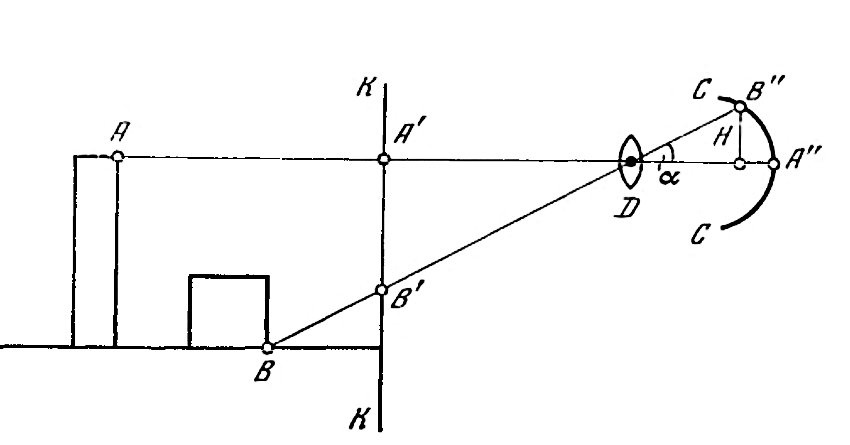
\includegraphics[width=0.8\linewidth]{figures/f1.1.png}
\end{figure}
\figblock{1.1}{Diagram illustrating that central projection onto picture plane $KK$ produces the same retinal image as direct retinal projection, for any retinal surface configuration.}

Consequently, quite independently of the configuration of the retinal surface, the system of
linear perspective ideally serves the purpose of obtaining coinciding retinal images of
external space and of the picture.

If one nevertheless wishes to consider the geometric proximity of the central projection onto
the picture plane $KK$ and onto the spherical surface $CC$, a useful sense of it is given by
comparing the segment $A'B'$ and the arc $A''B''$.  To make this comparison both lines must
be referred to the same scale, which ultimately reduces to comparing the arc-length $A''B''$
subtending visual angle~$\alpha$ and the perpendicular $H$ dropped from $B''$.  Numerically
the ratio of these lengths equals $2\alpha/\sin 2\alpha$ if the eyeball is taken to be
spherical.  This ratio depends strongly on~$\alpha$.  All manuals on the use of linear
perspective in artistic practice state that $\alpha$ should not exceed $15°$.  Another rule
given in drawing manuals specifies that the artist should depict an object from a distance no
less than three times the size of the object; in that case $\alpha < 10°$.  Similar values are
quoted in manuals on the psychology of visual perception as the angle~$\alpha$ corresponding
to sufficiently sharp vision.  This yields a negligibly small departure of arc-length from the
corresponding straight-line segment (of the order of 2--5\%), incomparably smaller than the
transformations brought about by the constancy mechanisms, which can reach hundreds of
per cent.

In view of the fundamental role played by the system of linear perspective here, let us present
the analytical relations belonging to it.  Adopt the following notation (Fig.\,1.2):
$H$---height of the viewpoint; $l_0$---distance from the viewpoint (the artist's eye) to the
picture plane; $b$---distance from the picture plane to the depicted point~$A$, lying in the
subject plane of the picture-space; $B$---distance of point~$A$ from the vertical plane
passing through the principal line of sight (the subject plane is taken to be horizontal);
$y_1$---distance to the image~$A_1$ of point~$A$ on the picture, measured from the base of
the picture plane; $x_1$---distance to the image~$A_1$ of point~$A$ on the picture, measured
from the principal axis of the picture.\footnote{All terms and definitions coincide with those
  given in the textbook by V.\,E.\,Peterson (V.\,E.\,Peterson, \emph{Perspective},
  Moscow, 1970).}

\begin{figure}[H]
    \centering
    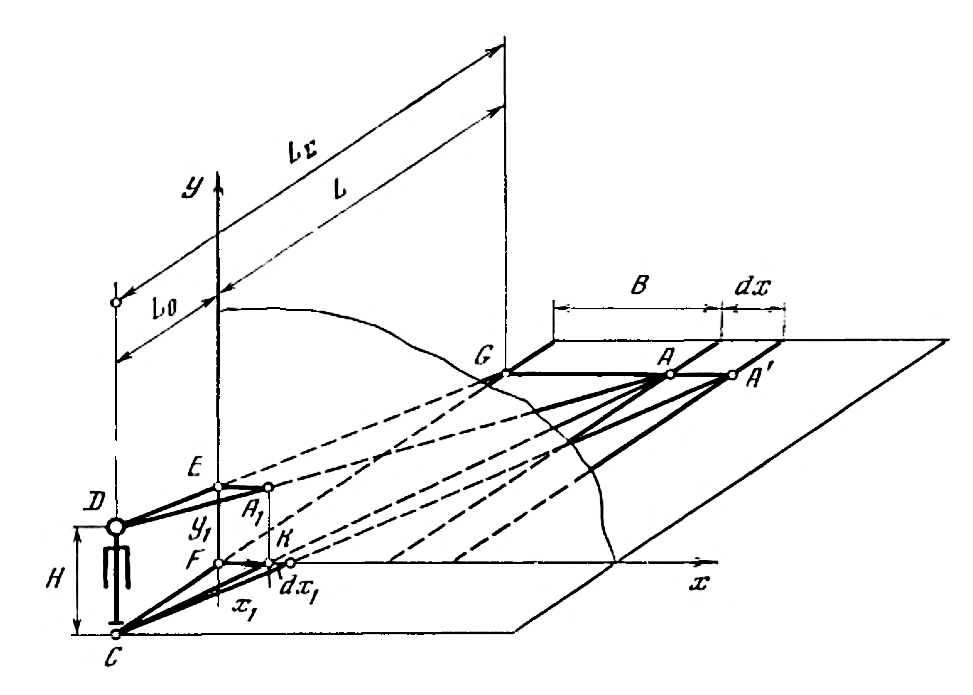
\includegraphics[width=0.9\linewidth]{figures/f1.2.png}
\end{figure}
\figblock{1.2}{Coordinate notation for the linear perspective construction: viewpoint at
  height $H$, picture plane $KK$ at distance $l_0$, depicted point $A$ at depth $b$
  and lateral offset $B$.}

\srcpage{245}

Suppose the problem is to depict a road with parallel edges of width $2B$
($B = \mathrm{const}$), whose axis of symmetry is perpendicular to the picture plane and
passes through the point in the subject plane where the artist stands.

Introduce dimensionless variables
\begin{equation}
  \overline{x} = -\frac{x}{b}, \qquad \overline{y} = \frac{y}{H}, \qquad \overline{l} = \frac{l}{l_0}.
  \tag{1.1}
\end{equation}

It is easy to verify that if the image~$A_1$ of point~$A$ is obtained by central projection
(linear perspective), then from the similarity of triangles $SBO$ and $PEO$ (Fig.\,1.2) there
follows the relation of ordinate~$y_1$ to the distance from point~$A$ to the picture plane:
\begin{equation}
  \overline{y_1} = \frac{l}{l_0 + l} = \frac{\overline{l}}{1+\overline{l}}.
  \tag{1.2}
\end{equation}

The subscript~$1$ here and below signifies that the image~$A_1$ of point~$A$ corresponds to
the system of linear perspective.  The similarity of triangles $SOA$ and $SPK$ allows one to
find the dependence of $x_1$ on~$b$, and with the use of formula~(1.2) to write the relation
between $y_1$ and $x_1$:
\begin{equation}
  \overline{x_1} = \frac{1}{1+\overline{l}},
  \tag{1.3}
\end{equation}
\begin{equation}
  \overline{y_1} = 1 - \overline{x_1}.
  \tag{1.4}
\end{equation}

The last expression says that the curve $y_1 = f(x_1)$ is a straight line; the image of the
road has its true width at the base of the picture plane (at $y_1 = 0$, $x_1 = 1$, i.e.\
$x_1 = B$) and zero width at the horizon line $y_1 = H$, since on that line $y_1 = 1$ and
consequently $x_1 = 0$.  The left edge of the road can be obtained from conditions of
symmetry.

If one takes some elementary segment $dx$ lying in the subject plane and parallel to the
picture plane, then consideration of triangle $CAA'$ shows that the projection of this
segment onto the picture plane will have size $dx_1$, where
\begin{equation}
  d\overline{x_1} = \frac{d\overline{x}}{1+\overline{l}}.
  \tag{1.5}
\end{equation}

Obviously, the size $dx_1$ is exactly the same if the elementary segment $dx$ is translated
parallel to itself to any location in the plane $b = \mathrm{const}$.

\srcpage{246}

% Appendix 2: The Possibility of Depicting Perceptual Space on a Plane
% Source pages: 247–253

\chapter{The Possibility of Depicting Perceptual Space on a Plane}

\srcpage{247}

The preceding Appendix showed that the system of linear perspective faithfully transmits the
geometry of the retinal image.  As is known (see Chapters\,II and\,III), the system of
perceptual perspective is obtained by transferring the geometric properties of perceptual
space onto the picture plane.  Two questions therefore arise: what are the geometric
properties of that space, and can it be depicted on a plane?

The geometric properties of perceptual space are obtained from the retinal image by
``stretchings'' and ``compressions'' of its elements under the action of the mechanisms of
size constancy and shape constancy.  Speaking of the character of the geometric
transformations associated with these two constancy mechanisms, one immediately sees
their fundamental difference.  The size-constancy mechanism changes the relative sizes of
visible objects depending on their distance from the observer.  Since the only variable on
which the numerical magnitude of the ``stretching'' or ``compression'' depends in this case
is the distance from the observer, one may regard the entire perceived space as subject to
these deformations, independently of which specific objects fill the picture-space.  The
shape-constancy mechanism acts only with respect to a specific object; without deforming
the remaining space, it is tied to that object, and therefore the character of the local
deformation changes when one object is replaced by another.

The system of perceptual perspective must take both effects into account.  Methodologically,
however, it is convenient to consider their action in succession: first the deformation of space
as a whole, then the local deformations associated with the existence of individual objects.
Under this approach one can speak of the system of perceptual perspective in the narrow
sense of the word, in which, when transforming the linear perspective, only the action of the
size-constancy mechanism is taken into account.  Without aiming to find here the specific
regularities of such a perspective system, let us consider the question of whether it is in
principle possible to transfer onto the picture plane the image that arises in human
consciousness---in such a way that the linear dimensions of the perceptual image are
consistent with the linear dimensions of its depiction on the canvas.

Fig.\,2.1 shows the picture plane $KK$, on which the image of the picture-space lying to the
left of $KK$ is obtained in the usual manner of linear perspective---by projecting objects from
some point $B$ located at height $BC$ above the subject plane.  Suppose that, as a result of
the action of the size-constancy mechanism, the apparent size of some object diminishes as it
recedes from the observer less rapidly than one would expect if the apparent size strictly
followed the retinal image.  A small segment $ds$ at point $A$, when projected from~$B$,
will have some characteristic linear size $ds_1$ on the picture plane.  Allowing for the action
of the size-constancy mechanism (and thereby departing from the system of linear
perspective), its image will have size $ds_2 = P\,ds_1$, where $P$~is some function relating
the size of the object as actually perceived by a person to the size that would result if
perception followed strictly from the retinal image.  The function $P$ depends on the distance
of the observed elementary segment from the observer: $l_\Sigma =l_0 + l$.  Since the quantity $l_0$ is
constant, it is convenient to write the function $P$ in the form $P(l)$ or, passing to the
dimensionless variables introduced by relations~(1.1), in the form $P_1(\overline{l})$.

\begin{figure}[H]
    \centering
    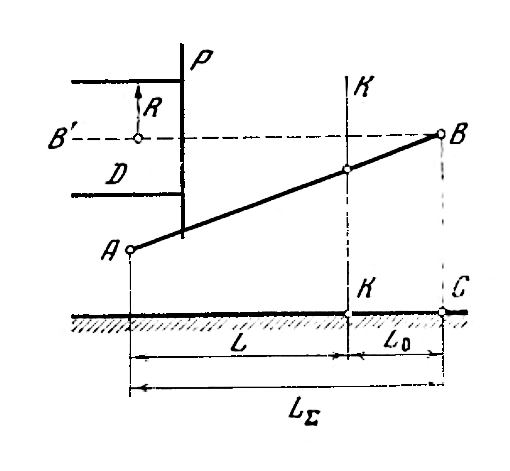
\includegraphics[width=0.5\linewidth]{figures/f2.1.png}
\end{figure}
\figblock{2.1}{Geometry of the perceptual-perspective construction: picture plane $KK$,
  centre of projection $B$ at height $BC$, and the function $P_1(l)$ relating perceptual
  to retinal image sizes.}

It is convenient to begin determining the basic properties of the function $P_1$ by equalising
the scales of the two perspective systems: linear and perceptual.  To this end we assume that
the segment $d\overline{s}$ lies in the picture plane, so $d\overline{s}_1 = d\overline{s}$.  We agree to consider that in the
picture plane (at $b = 0$) the apparent and true sizes coincide, i.e.\ for $l = 0$:
$d\overline{s} = d\overline{s}_1 = d\overline{s}_2$.  Thus for $\overline{l} = 0$, $P_1(0) = 1,$ while for all other distances from the observer. \footnote{For constant $L$ (points at equal
  distance from the picture plane), expression~(2.1) can obviously be written in finite
  form: $x_2 = P_1(L)\,x_1$.}

\srcpage{248}
\begin{equation}
  dx_2 = P_1(l)\,dx_1.
  \tag{2.1}
\end{equation}

In expression~(2.1) the notation has been refined by the transition from $ds$ to $dx$, since
we introduce the assumption that the segment $ds$ is horizontal and parallel to the picture
plane, i.e.\ it coincides with $dx$.

Differentiating equality~(2.1) with respect to $l$, using expression~(1.5) and treating $dx$
as constant:
\begin{equation}
  \frac{d}{dl}dx_2 = \frac{dx}{1+l}\frac{d}{dl}P_1(l) - P_1(l)\frac{dx}{(1+l)^2}
  \tag{2.2}
\end{equation}
where $P_1' = dP_1/dl$.

If one makes the assumption of complete constancy at small distances from the observer
(which is practically always the case), then for sufficiently small $l$ (i.e.\ for a picture
plane sufficiently close to the observer) the size $dx_2$ in the immediate neighbourhood of
the picture plane should not change with increasing~$b$.  Analytically this is expressed by
the condition $\frac{d}{dl}dx_2 = 0$, which on the basis of equality~(2.2) allows one to find a
further condition that the function $P_1(l)$ must satisfy [taking into account the earlier
condition $P_1(0) = 1$]:
\begin{equation}
  \frac{dP_1}{dl}(0)=\left.\frac{P_1(l)}{1+l}\right|_{0} = 1.
  \tag{2.3}
\end{equation}
\vspace{-12pt}
\begin{figure}[H]
    \centering
    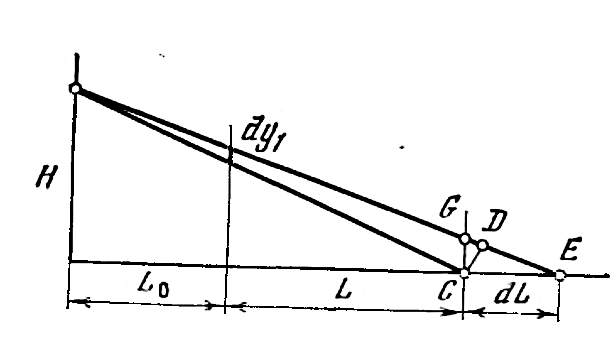
\includegraphics[width=0.6\linewidth]{figures/f2.2.png}
\end{figure}
\figblock{2.2}{Diagram for establishing the relation between the depth increment $dl$ and
  the vertical image increment $dy_1$.}

At $l \to \infty$, i.e.\ at the horizon line, $dx_2 = 0$ regardless of the size of $dx$.  This
is a natural result of the fact that at a sufficiently large distance any object of finite size
will be seen as a point, since its angular size will become so small that it will be able to
excite only a single photoreceptor of the retina.  At $l \to \infty$ the linear perspective
already gives $dx_1 = 0$, and consequently it is sufficient to require that the function
$P_1(\infty)$ be finite, i.e.\ that $P_1(l)$ have a finite upper bound.  Everyday visual
experience testifies to the continuity of the function $P_1(l)$, since, when observing railway
tracks, for example, no one has seen a jump discontinuity in their apparent width at some
distance.  Almost equally evident is the monotonicity of the function $P_1(l)$.  This is
connected with the reasonableness of a uniform response of the human perceptual system
to a uniform stimulus---in the present case, to an increase in distance~$l$.  The monotonicity
of $P_1$ together with the conditions $P_1(0) = 1$ and $dP_1/dl(0) = 1$ allows one to write
$P_1(l) \ge 1$.  Obviously, an infinite family of functions can satisfy the described properties,
and the choice of an appropriate function should be made taking into account experimental
data, the required accuracy, and simplicity of expression in elementary functions.

The function $P_1(l)$ allows one to find the apparent width of element $dx$, or of the road
discussed at the end of the preceding Appendix, if the corresponding image in the system of
linear perspective is known; however, the size-constancy mechanism will change not only
the $x$-coordinate but also~$y$.

Fig.\,2.2 shows the construction enabling one to establish the relation between an increment $dl$ and $dy_1$. 
\begin{equation*}
    dy_1 = \frac{l_0}{l_0+l} \ \frac{H}{l_0+l}dl
\end{equation*}

Differentiating [equation~(1.2)]:
\begin{equation}
  dy_1 = \frac{dl}{(1+l)^2}.
  \tag{2.4}
\end{equation}

\srcpage{249}

The quantity $dy_1$ can be regarded as the image on the picture plane, by the laws of linear
perspective, of a segment $SD$ perpendicular to the line of sight.  The function $P_1(l)$
introduced above transformed some width in linear perspective into another corresponding
to visual perception.  This allows one to transform the image of segment $SD$ by the same
law.  By this assumption the claim is introduced that all segments lying in the plane normal
to the line of sight are transformed by one and the same law: this is natural, for otherwise
the visible image of a flat square normal to the line of sight would, as it recedes from the
observer, transform into a different figure, which no one has observed.  But then
\begin{equation}
  dy_2 = P_1(l)\,dy_1,
  \tag{2.5}
\end{equation}
and consequently, on the basis of equation~(2.4):
\begin{equation}
  y_2 = \int_0^l \frac{P_1(l)}{(1+l)^2}\,dl.
  \tag{2.6}
\end{equation}

Let us return to Fig.\,2.1 and consider the image of some figure lying in the plane~$P$,
parallel to the picture plane $KK$ and located at distance $l_P$ from it.  Since for all
points of plane~$P$, $P_1(l_P) = \mathrm{const}$, the transformation that the image of the
figure undergoes when passing from the linear to the perceptual perspective system will be
a similarity transformation.  Suppose now that in plane~$P$ there lies the rim of an
infinitely extended hollow cylinder~$\Pi$ of radius~$R$ with its axis lying on the line $BB'$.
Then on the picture plane $KK$, under projection from point~$B$ (i.e.\ in the system of
linear perspective), the cylinder will map to a circle centred at the principal point of the
picture, and its infinitely distant end will be represented by that centre.  The image of the
near rim of the cylinder will have radius $r_1 = R\,l_0/(l_0 + l_P) = R/(1+l_P)$.  Let us
ask what the image of this same cylinder will be in the system of perceptual perspective.
Obviously its rim will also appear as a circle centred at the principal point of the picture,
and that centre will simultaneously be the image of its infinitely distant end.  The radius of
the circle representing the near end of the cylinder will be $r_2 = r_1 P_1(l_P)$, and the
image of the cylinder's generator receding to infinity, on the picture plane in the system of
perceptual perspective, will by equality~(2.6) have size\footnote{Not shown in the figure.}

\srcpage{250}
\begin{equation}
  l_2 = \int_{l_P}^{\infty} \frac{P_1(l)}{(1+l)^2}\,dl.
  \tag{2.7}
\end{equation}

Let us compare $l_2$ and $r_2$.  With the expression for $r_1$:
\begin{equation}
  r_2 = \frac{R\,P_1(l_P)}{1+l_P}.
  \tag{2.8}
\end{equation}

If one were to assume that under the integral sign in~(2.7) stood not $P_1(l)$ but the
constant value $P_1(l_P)$, it would be easy to verify that $l_2 = r_2$.  Since, however, for
$l > l_P$ the monotonically increasing character of $P_1(l)$ gives $P_1(l) > P_1(l_P)$, it
is evident that
\begin{equation}
  l_2 > r_2.
  \tag{2.9}
\end{equation}

The inequality obtained shows the in-principle impossibility of depicting the considered
cylinder in the system of perceptual perspective.  Indeed, the image of the cylinder's
generator must have one end at the image of the infinitely distant point---i.e.\ at the centre
of the circle of radius~$r_2$---and the other end on that circle.  Since from point~$B$ only
the inside of the cylinder is visible, all points of the image of its surface must lie inside the
circle of radius~$r_2$.  But since $l_2 > r_2$, the images of the near ends of the generators
will not lie on the circle but will fall outside it, which is impossible as it contradicts the
preceding condition.

As is known, to prove some proposition one must show that it holds always, while to refute
it, it suffices to give a single counter-example.  The considered example of depicting a
hollow cylinder therefore refutes the view (if it existed) that the perceptual perspective
system is capable of serving as a representation of any body.  In contrast, the system of
linear perspective, which reduces to projecting from point~$B$ objects in the picture-space,
is capable of transmitting the projection of any object onto the picture plane (although for
large visual angles this formally correct image will convey the visual impression in a
strongly distorted form).

The in-principle inability of the perceptual perspective system to represent any arbitrary
object on the picture plane requires the identification of the class of objects whose
depiction in the system of perceptual perspective is possible.  The monotonically increasing
function $P_1(l)$ has a finite upper bound, which leads to the practical constancy of $P_1(l)$
starting from some sufficiently large value of~$l$.  But then for the distant regions of space
the image in the perceptual perspective system is similar to the image in the linear
perspective system, i.e.\ always possible.  In exactly the same way, figures lying in planes
parallel to the picture are depictable; as noted above, they are obtained from the linear
perspective system by a similarity transformation.

Let us finally give one more case---the depiction of a comparatively narrow portion of a
plane parallel to the axis $BB'$.  Such a portion, even if it begins at the picture plane and
has infinite extent in depth, can be consistently depicted on the picture plane, since its
transformations (which, as is evident from the foregoing, have the character of stretching)
in the ``receding'' direction and in the lateral direction are independent.  By virtue of this
independence, the occurrence of a contradiction of the kind discussed in connection with the
cylinder is impossible (in the above example, the quantity~$l_2$, directed ``away from the
observer'', and the quantity~$r_2$, directed laterally, were linked by the unfulfilable
requirement $r_2 = l_2$).

\srcpage{251}

Thus the depiction of nearby portions of planes parallel to the picture, perpendicular to it,
and horizontal, in the system of perceptual perspective is possible.  Precisely such portions
of planes most frequently occur in depicting various rectangular objects.  Since, by what has
been said, the depiction of such portions is feasible, one should consider whether the
perceptual perspective system can be used to represent the spatial objects composed of them.
Let us consider in this connection two typical cases.

\smallskip
\textit{Case~I.  Depiction of an interior (a parallelpiped seen from inside).}
Fig.\,2.3 shows the projection of some interior onto the picture plane, i.e.\ its image in the
system of linear perspective.  Let the bounding rectangle have area~$S_1$; this rectangle
represents the cross-section of the parallelpiped closest to the observer---as it were, the
``entrance'' to the interior.  Let this section correspond to some value $l = l_P$, while all
other planes bounding the interior-space will naturally lie at $l > l_P$.  Write the obvious
identity
\begin{equation}
  S_1 = \iint_{s_1} dx_1\,dy_1,
  \tag{2.10}
\end{equation}
which gives the area of the ``entrance'' in the system of linear perspective.

On the basis of relations~(2.1) and~(2.5), $dx_2\,dy_2 = P_1^2(l)\,dx_1\,dy_1$.  Then
\begin{equation}
  S_2 = \iint_{s_1} P_1^2(l)\,dx_1\,dy_1,
  \tag{2.11}
\end{equation}
where $S_2$ is the area bounded by the contour of the image in the system of perceptual
perspective.

\begin{figure}[H]
    \centering
    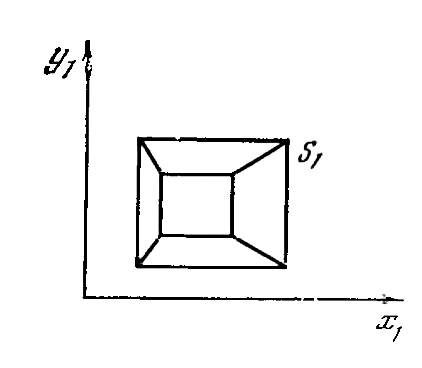
\includegraphics[width=0.3\linewidth]{figures/f2.3.png}
\end{figure}
\figblock{2.3}{Projection of an interior (parallelpiped seen from inside) onto the picture
  plane in linear perspective.  The outer contour serves simultaneously as the boundary of
  the ``entrance'' plane and of the walls, floor, and ceiling.}

However, the outer contour of the interior shown in Fig.\,2.3 has two meanings: first, it
bounds the image of the ``entrance'' plane, and second, it bounds the images of the walls,
floor, and ceiling.  In the first case the perceptual image should correspond to the area
\begin{equation}
  S_2' = P_1^2(l_P)\iint_{s_1} dx_1\,dy_1 = P_1^2(l_P)\,S_1,
  \tag{2.12}
\end{equation}
and in the second to the area
\begin{equation}
  S_2'' = \iint_{s_1} P_1^2(l)\,dx_1\,dy_1,
  \tag{2.13}
\end{equation}

\srcpage{252}

where the values of $l$ are taken for the corresponding boundary points of the interior.  By
virtue of the properties of $P_1(l)$ stated above and the fact that in the case under
consideration $l > l_P$, one obtains the inequality
\begin{equation}
  S_2'' > S_2',
  \tag{2.14}
\end{equation}
which, like inequality~(2.9), testifies to the impossibility of depicting an interior in the
system of perceptual perspective, even though each wall, floor, and ceiling individually
can be depicted.

\begin{figure}[H]
    \centering
    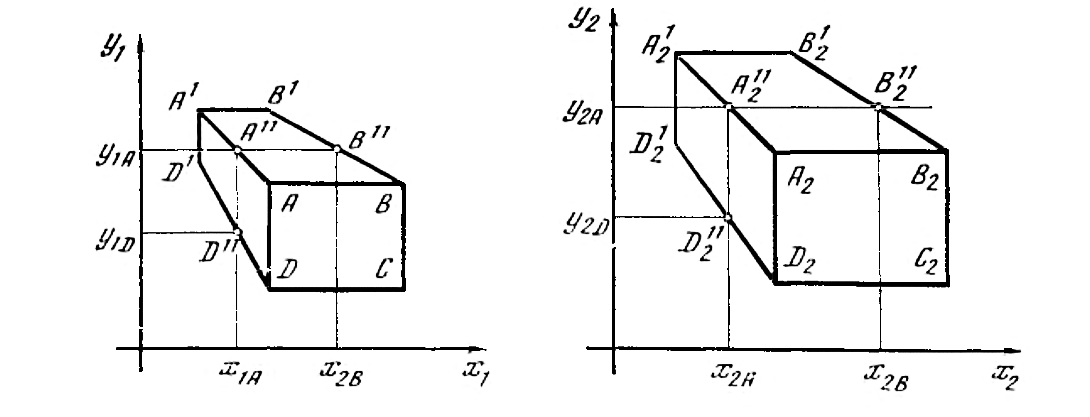
\includegraphics[width=0.8\linewidth]{figures/f2.4.png}
\end{figure}
\figblock{2.4}{The same parallelpiped shown twice: left in linear perspective, right in
  perceptual perspective.  The perceptual image of the nearest face is enlarged by factor
  $P_1(l_P) > 1$; lateral faces undergo a more complex transformation.}

\textit{Case~II.} Depiction of a parallelpiped with faces parallel to the coordinate planes, seen from outside. Fig.\,2.4 shows such a depiction twice: on the left in the system of linear perspective, on
the right in the system of perceptual perspective.  Let the face of the parallelpiped nearest
to the observer be at distance $l_P$ from the picture plane.  Since the passage to the
perceptual image, as already noted, involves for such planes a similarity transformation, the
perceptual image of face $A_2B_2C_2D_2$ will differ from the face $ABCD$ obtained by
central projection only in scale---it will be larger, since $P_1(l_P) > 1$.  The lateral
faces $ABB'A'$ and $ADD'A'$ will be transformed in a more complex manner, since the
function $P_1(l)$ will not be constant for them.  Let the $y$-axis be the trace of the section
of the picture plane by the vertical plane passing through the centre of projection and
containing the line perpendicular to the picture plane.  Then for each given $l = l_1$:
\begin{equation}
  y_{1A} = H - \frac{H_1}{1 + l_1},
  \tag{2.15}
\end{equation}
where $H$ is the height of the viewpoint and $H_1$ is the distance from the centre of
projection to the plane containing face $ABB'A'$.

The horizontal line $y_1 = y_{1A}$ will intersect the image of face $ABB'A'$ at points $A''$
and $B''$.  The image shown on the right of the parallelpiped can be constructed as follows.
Let the image of edge $A_2A_2'$ already be built in one way or another.  Taking the
point~$A_2$ on it corresponding to~$A''$, and drawing a horizontal line through it, lay off
on it the distance determining the position of point~$B_2$ corresponding to~$B''$:
\begin{equation}
  x_{2B} - x_{2A} = \bigl(x_{1B} - x_{1A}\bigr)\,P_1(l_1),
  \tag{2.16}
\end{equation}
and the vertical segment
\begin{equation}
  y_{2A} - y_{2D} = \bigl(y_{1A} - y_{1D}\bigr)\,P_1(l_1),
  \tag{2.17}
\end{equation}
measured from point~$A_2$, will determine the position of the corresponding point.

In such a construction no manifest contradictions arise [of the type of relations~(2.9)
and~(2.14)], since the construction of points $B_2$ and $D_2$ is independent (directed in
``different directions'') and not bounded by any conditions.

Nevertheless, the resulting image will carry a distortion of the visual impression.  One can
show that the found distance of point~$D_2$ from the horizontal through~$A_2$, and its
distance from the horizontal through~$D_2$ (obtainable by starting the construction
directly from~$D_2$ rather than via~$A_2D_2B_2$), will turn out to be inconsistent---they
will not sum to the distance between $A_2B_2'$ and $D_2C_2$.  This is further aggravated
by the already noted impossibility, discussed in Chapter~III, of an image correctly
transmitting the three simultaneously visible angles at a vertex of a parallelpiped.  Thus a
flawless depiction of a parallelpiped ``from outside'' is likewise impossible, although the
errors thereby arising are less conspicuous.

%\srcpage{253}

% Appendix 3: Quantitative Relationship Between Linear and Perceptual Perspective
% Source pages: 253–256

\chapter{Quantitative Relationship Between Linear and Perceptual Perspective}

\srcpage{253}

The equations obtained above hold for a function $P_1(l)$ of any form.  In order to pass
to a quantitative comparison of linear and perceptual perspectives, we choose this function
as follows:
\begin{equation}
  P_1(l) = 1 + \arctan l.
  \tag{3.1}
\end{equation}

\srcpage{254}

It is easy to verify that the chosen function satisfies all the conditions enumerated above:
it is continuous and monotone, $P_1(0) = 1$, $P_1(\infty) = 1 + \pi/2$, and
\[
  \left.\frac{dP_1}{dl}\right|_{l=0} = \frac{1}{1+l^2}\bigg|_{l=0} = 1.
\]
Thus the function $P_1(l) = 1 + \arctan l$ qualitatively satisfies the stated properties;
its quantitative correspondence to visual perception can be confirmed only by experiment.

Fig.\,3.1 shows the dependences $y_1 = f_1(x_1)$ and $y_2 = f_2(x_2)$.  The first is
obtained from equation~(1.4), and the second by means of equations~(2.1) and~(3.1).  If
the first dependence gives the linear-perspective image of the right edge of a road, the
second is a mixed dependence: the quantity~$y$ is taken for linear perspective and $x$~for
perceptual perspective.  Such a mixed dependence does not represent the perceptual
perspective, but it does allow one to estimate easily the effect of the size-constancy
mechanism: the values of the abscissae $x_1$ and $x_2$ corresponding to the same value
of~$y_1$ also correspond to the same value of~$l$, and consequently their ratio gives a
clear representation of the contribution of the constancy mechanism to the process of
transforming the retinal image into the perceptual one.  Also shown in Fig.\,3.1 are
experimental points, which testify to a sufficiently good quantitative agreement of the
chosen dependence $P_1(l) = 1 + \arctan l$ with the data of human visual perception.

\begin{figure}[H]
    \centering
    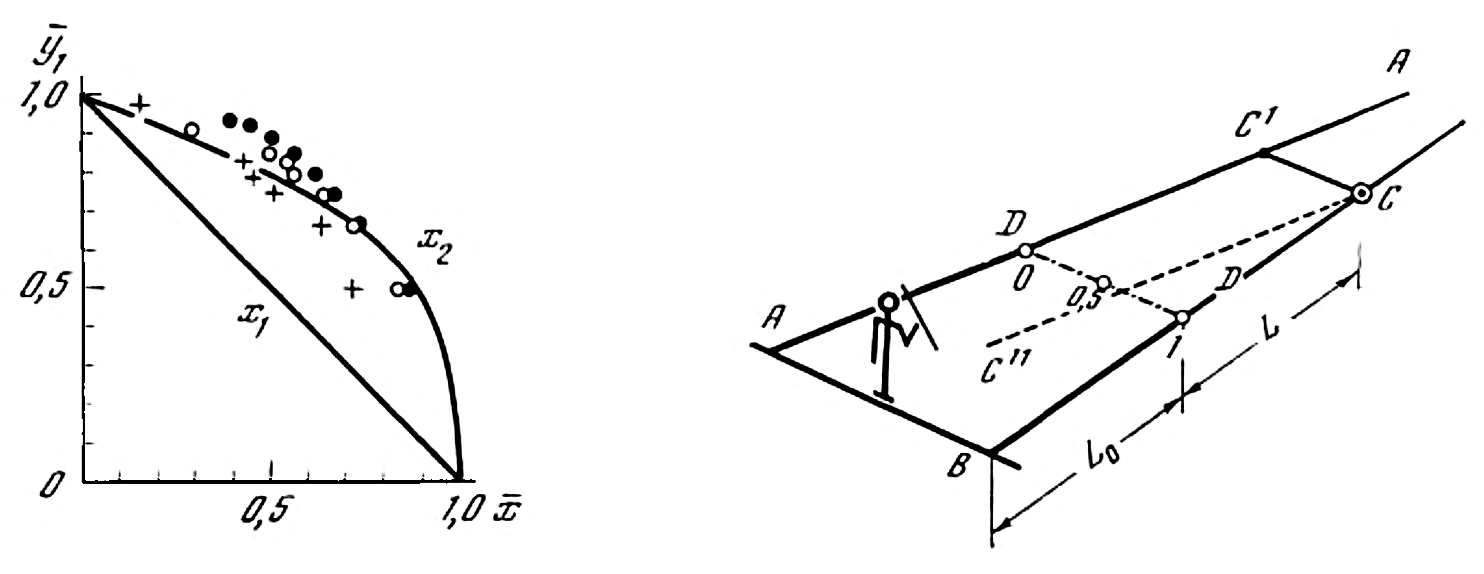
\includegraphics[width=0.95\linewidth]{figures/f3.1-f3.2.png}
\end{figure}
\figblock{3.1}{Comparison of the linear-perspective edge curve $y_1 = f_1(x_1)$ and the
  mixed perceptual curve $y_2 = f_2(x_2)$ for the right edge of a road, together with
  experimental points (filled circles: path width 1\,m; open circles: 2\,m; crosses: 5\,m).}
\figblock{3.2}{Scheme of the experiment for measuring the apparent width $x_2$ at various
  distances from the observer.  The experimenter aligns the ruler edge through object~$C$
  so that it appears parallel to the left edge $AA$ of the path; the scale $OO$ gives $x_2$
  directly.}

In order to make clear the degree of reliability of the experimental results cited, let us
describe the methodology of the experiment for measuring the quantity~$x_2$.  Since the
problem being solved is that of obtaining an image of a straight road, the experiment was
conducted in the field by measuring the apparent width of a road at various distances from
the observer.  The experimental methodology was designed so as to measure precisely the
apparent width, not the retinal image.

\srcpage{255}

Fig.\,3.2 shows the scheme of the experiment.  At a distance $l_0$ from the experimenter,
standing at the midpoint of a narrow straight path and looking along it, a line is drawn on
the surface of the path perpendicular to its axis and marked in fractions of the path's width.
Along the right edge of the path, at a previously known distance~$l$, some visible small
object~$C$ is placed.  Holding a ruler and looking with one eye, the experimenter aligns
the edge of the ruler with the object~$C$, which is at distance $l_0 + l$ from him.  The
task is that the edge of the ruler passing through~$C$ should appear parallel to the left
edge $AA$ of the path (the trace of the ruler's edge on the ground is shown by the dashed
line $CC''$).  Having achieved this, the experimenter takes a reading on the scale $OO$
along the ruler's edge and thereby determines the apparent size of the width $CC'$ in
relation to the size $OD$, taken as unity.  Obviously, the reading on the scale $OO$
directly gives the value of~$x_2$.  By moving object~$C$ (varying~$l$), one obtains the
dependence of $x_2$ on~$l$, and then via formula~(1.2) on~$y_1$.  These are precisely the
points plotted in Fig.\,3.1.\footnote{If the experimenter had measured the segment $CC'$
  by aligning the measuring device with both $C$ and $C'$ and then transferring that size
  to the segment $OD$ to assess its magnitude as a fraction of the road's width (as is
  sometimes done when learning to draw), the experimental points in Fig.\,3.1 would have
  fallen not near the curve $x_2$ but near the straight line $x_1$, i.e.\ they would have
  corresponded to linear perspective, since the alignment of points always occurs at the
  retinal level.}

The conviction that the adopted methodology makes it possible to measure the apparent
rather than the retinal image follows from the fact that the measuring device (the ruler) is
aligned with only one point~$C$ (this alignment is, of course, connected with alignment on
the retina of the eye), while instead of aligning the device with point~$C'$ to measure
segment $CC'$, a line $CC''$ parallel to $AA$ is constructed.  Since line $CC''$ is
constructed parallel to the apparent direction of $AA$ without aligning the measuring device
with any point of line $AA$, this construction takes place not at the retinal but at a higher
level of the human visual-perception system.

\srcpage{256}

The experimental points shown in Fig.\,3.1 were obtained under the following conditions:
path width 1\,m, $l_0 = 1$\,m, $l$ varied from 1 to 15\,m (marked by filled points); width
2\,m, $l_0 = 2$\,m, $l$ varied from 2 to 24\,m (marked by open circles); width 5\,m,
$l_0 = 5$\,m, $l$ varied from 5 to 180\,m (marked by crosses).  Comparison of the
experimental data and the conditionally adopted theoretical relation indicates that the latter
gives, on the whole, a qualitatively correct representation of the dependence $x_2 = f(l)$.
A noticeable departure of the experimental points from the curve, which gives values of the
function $P_1(l)$ that are too low, can be noted only for large~$l$ (values of $y_1$ close
to~1).

The comparatively good quantitative agreement of the law of variation of $x_2$ obtained
on the basis of $P_1(l) = 1 + \arctan l$ with the experimental data does not yet mean that
a general law of variation of $P_1$ with~$l$ has been found.  Nevertheless, the general
character of the variation of $x_2$ as a function of~$l$ is correctly conveyed.  In the
present book only the most general qualitative comparison of linear and perceptual
perspective is carried out, and therefore a quantitatively exact knowledge of the
dependence $P_1(l)$ is not necessary.  This is precisely what allows one to use in the
calculations the function $P_1(l)$ given by formula~(3.1).  Another consideration in favour
of formula~(3.1) is that it gives a good quantitative agreement with experiment also for
comparatively small~$l$ (in the case under consideration $l_0 = 2$\,m), and in particular
for a very close foreground, which is important in the analysis of medieval pictorial art.

Having the function $P_1(l)$ given by formula~(3.1), and using formula~(2.1) and
equation~(2.6), the perceptual image of the road can be computed.  For the adopted
function, equation~(2.6) takes the closed form
\begin{equation}
  y_2 = \int_0^l \frac{1 + \arctan(l)}{(1+l)^2} dl 
      = \frac{1}{4}\ln\frac{(1+l)^2}{1+l^2}+\frac{l-1}{2(1+l)}\arctan(l)
      + \frac{l}{1+l} \, ,  
  \tag{3.2}
\end{equation}
Using this formula one can construct the perceptual image of the road (shown as the right
image in Illustration~17 of the main text).

\begin{figure}[H]
    \centering
    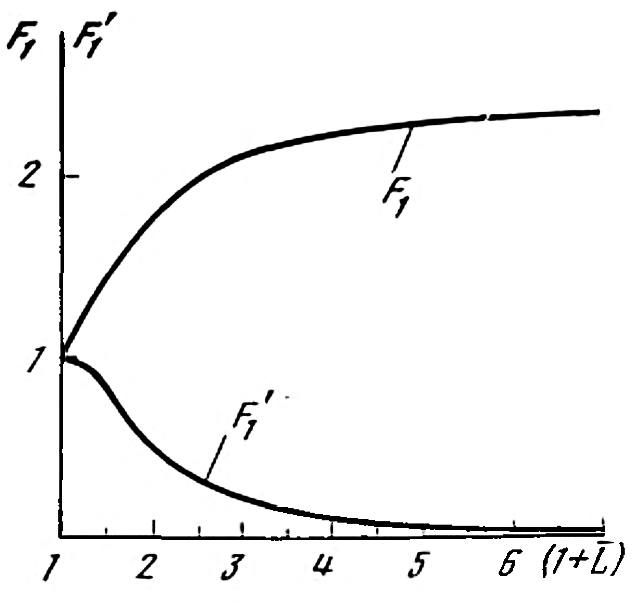
\includegraphics[width=0.4\linewidth]{figures/f3.3.png}
\end{figure}
\figblock{3.3}{Graphs of $P_1(l) = 1 + \arctan l$ and $P_1'(l) = 1/(1+l^2)$ as functions
  of the total distance $1 + l$ from the observer. $P_1$ shows the enlargement of the retinal
  image at depth $l$; $P_1'$ shows the rate of non-uniformity of that stretching.}

In conclusion it is useful to make several additional remarks.  Formula~(3.1) shows that
while for small and medium values of~$l$ the function $P_1(l)$ changes with~$l$, for
large~$l$ the value of $P_1(l)$ becomes practically constant and equal to $1 + \pi/2$.
This means that from some sufficiently large distance onward, linear and perceptual
perspectives differ only in scale: with the adopted form of $P_1(l)$, the perceptual
perspective is $1 + \pi/2 \approx 2.6$ times larger than the linear, but geometrically
similar to it.  In accordance with formula~(1.2), $y_1 \to 1$ as $l \to \infty$, while
for $P_1(l) = 1 + \arctan l$, formula~(3.2) gives

\[
  y_2 \;\xrightarrow{l\to\infty}\; 1 + \frac{\pi}{4} \approx 1.79,
\]
that is, the depth-image of space in perceptual perspective in this case is almost twice as
large as in linear perspective.

A characteristic feature of the transformation from linear to perceptual perspective (i.e.\
from the retinal image to perceptual space) is its continuity: in the course of this
transformation no gaps or discontinuities arise.  The transformation proceeds as a
``stretching''---non-uniform, to be sure, but unconditionally continuous.  Having the
specific form~(3.1) of the function $P_1(l)$, one can construct graphs relating $P_1(l)$
and $P_1'(l)$ as functions of $1 + l$ (distance from the observer); these are shown in
Fig.\,3.3.  The curve $P_1'(l)$ conveys the character of the ``stretching'' of the retinal
image: the larger this quantity, the more non-uniform the stretching of the retinal image,
which can appreciably change the geometric form of the contemplated object in the
transition from the retinal image to perceptual space.  The tendency of $P_1'$ to zero
indicates that the retinal image and the image arising in perceptual space are
geometrically approaching each other.  The curve $P_1(l)$ gives the enlargement factor of
the retinal image in the transition to perceptual space.

Taken together, both graphs show that the near zone is characterized by a significant
change by the visual-perception system in the geometric form of the object's retinal
projection without a strong change in its size, while for more distant regions of space one
observes a simple ``stretching'' of the corresponding retinal image without change of form.
This circumstance explains why, beginning from some distance, the system of linear
perspective gradually becomes natural.

In Appendix~2 the in-principle impossibility of depicting perceptual space on the picture
plane was demonstrated, yet in Illustration~17 this was done.  There is in fact no
contradiction between the statements of Appendices~2 and~3.  The point is that the image
of a road is not an image of space, because in objective space the entire road lies in the
subject plane.  Consequently, Illustration~17 gives the linear and perceptual perspectives
of the subject \emph{plane}, not of subject \emph{space}.

% Appendix 4: Axonometry
% Source pages: 257–260

\chapter{Axonometry}

\srcpage{257}

Axonometry is a special case of both the linear-perspective system and the perceptual
system.  For the first this is a well-known fact; for the second it follows at least from the
observation that for distant regions of space both perspective systems are geometrically
similar.  Let us examine the related questions in more detail.

To assess the degree of axonometric character of an image, introduce the quantity~$\Delta$,
defined as the relative change in width of an object with increasing depth (i.e.\ increasing
distance from the picture plane to that object).  Taking the road width from Appendix~3 as
the basis of the calculation, one can form two functions $\Delta$:
\begin{align}
  \Delta_1 &= (x_1' - x_1'')/x_1', \tag{4.1a} \\
  \Delta_2 &= (x_2' - x_2'')/x_2'. \tag{4.1b}
\end{align}
Here $x_1'$ and $x_2'$ are the road widths in the linear and perceptual perspective systems
respectively at distance~$l$ from the picture plane, and $x_1''$ and $x_2''$ are the same
widths at distance $l + \delta$ from the picture plane.  Thus the quantities $\Delta_1$ and
$\Delta_2$ characterise the degree of axonometric character of a region of depth~$\delta$
beginning at distance~$l$ from the picture plane.  In the case of ideal axonometry the road
width does not change with depth (i.e.\ $x'' = x'$), and for the function~$\Delta$ the
equality
\begin{equation}
  \Delta = 0 \tag{4.2}
\end{equation}
holds, which is the criterion of ideal axonometric character.  If $\Delta \neq 0$, the degree
of closeness to axonometry may be judged by how close $\Delta$ is to zero.

Based on formulas~(1.1) and~(1.3), one can write

\srcpage{258}
\begin{equation}
  \Delta_1 = \frac{\delta}{1 + l + \delta},  \tag{4.3}
\end{equation}
where $\delta = \Delta/l_0$.  Supplementing these with formula~(2.1), it is not difficult to
find
\begin{equation}
  \Delta_2 = \Delta_1 - \frac{\delta\,P_1'(l)}{(1+l)\,P_1(l)}.  \tag{4.4}
\end{equation}
In the last expression it has been assumed that the depth~$\delta$ is sufficiently small,
so that only the linear part of the increment of $P_1$ is taken into account.

Comparing the expressions for $\Delta_2$ and $\Delta_1$, and taking into account that the
function $P_1$ is monotonically increasing ($P_1' > 0$), one immediately obtains the
inequality
\begin{equation}
  \Delta_2 < \Delta_1,  \tag{4.5}
\end{equation}
which says that the perceptual perspective of any thin-depth object is more axonometric
than its linear perspective.  Since the perceptual perspective correctly transmits the actual
properties of visual perception, one can assert that the geometry of human visual perception
is always more axonometric than the retinal image.

Let us find the regions of picture-space that will be characterised by ideal axonometry.
Suppose a thin-depth object (of depth~$\delta$) is given and we move it ``away'' in the
direction of increasing~$l$, starting from $l = 0$.  As follows from formula~(4.3),
axonometry in the linear perspective arises only as $l \to \infty$ (it is only then that
$\Delta_1 \to 0$).  This corresponds to the well-known property of the linear perspective
system, for which strongly receding thin-depth planes are axonometric.

This is also true for the perceptual perspective system.  Indeed, as $l \to \infty$ the second
term of expression~(4.4) also tends to zero, since the monotonically increasing function
$P_1(l)$ has a finite upper bound (see Appendices~2 and~3), and consequently
$\Delta_2 \to 0$ as $l \to \infty$.

Moreover, the equality $\Delta_2 = 0$ holds also in the region of space immediately
adjacent to the picture plane ($l = 0$).  Indeed, in this region the first term of~(4.4)
equals $\delta/(1+\delta)$, while the ratio $P_1'/P_1 = 1$ at $l=0$ (from the properties of
$P_1$ discussed in Appendix~2: $P_1(0) = 1$ and $P_1'(0) = 1$).

\srcpage{259}

Thus, in contrast to the system of linear perspective---which becomes axonometric only for
thin-depth spatial layers receding ``to infinity''---the system of perceptual perspective
becomes axonometric twice: not only for very distant regions of space, but also for a
thin-depth region immediately adjacent to the picture plane.

\begin{figure}[H]
    \centering
    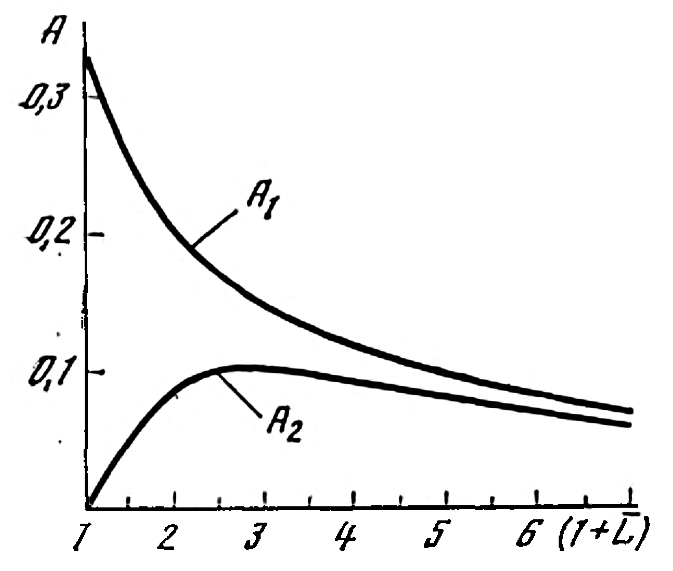
\includegraphics[width=0.45\linewidth]{figures/f4.1.png}
\end{figure}
\figblock{4.1}{Graphs of $\Delta_1$ and $\Delta_2$ as functions of $1+l$, computed from
  formulas~(4.3) and~(4.4) with $\delta = 0.5$ and $P_1(l) = 1 + \arctan l$.  The curve
  $\Delta_2$ lies everywhere below $\Delta_1$ (inequality~4.5) and satisfies $\Delta_2 = 0$
  both at $l=0$ and as $l\to\infty$, while $\Delta_1 = 0$ only as $l\to\infty$.}

Fig.\,4.1 shows the variation of $\Delta_1$ and $\Delta_2$ computed from formulas~(4.3)
and~(4.4) for $\delta = 0.5$, using the specific form of $P_1(l)$ given by formula~(3.1).
The graphs show that the convergence of curves $\Delta_1$ and $\Delta_2$ occurs somewhere
in the region $1 + l \approx 4$ and becomes increasingly complete as $l$ grows.  This
testifies to the similarity of the linear and perceptual perspective systems for distant
regions of space.  The overall behaviour of the curves also shows that $\Delta_1 \to 0$ and
$\Delta_2 \to 0$ only as $l \to \infty$, while in contrast to $\Delta_1$ the function
$\Delta_2 = 0$ already at $l = 0$.  The curve $\Delta_2$ lies everywhere below $\Delta_1$,
illustrating inequality~(4.5).

\srcpage{260}

If one recalls that the perceptual perspective system correctly transmits the numerical
characteristics of the geometric images arising in human consciousness, then the divergence
of curves $\Delta_1$ and $\Delta_2$ (especially for small~$l$) testifies to the departure of
the geometry of the linear perspective system from the geometry of visual perception.

% Appendix 5: The Occurrence of Reverse Perspective at Close Distances
%             due to the Phenomenon of "Superconstancy"
% Source pages: 260–262

\chapter{The Occurrence of Reverse Perspective at Close Distances due to
  the Phenomenon of ``Superconstancy''}

The size-constancy mechanism is sufficiently effective that over limited distances complete
constancy is frequently observed.  In the classic experiments of Holway and
Boring,\footnote{A.\,H.~Holway, E.\,G.~Boring.  Determinants of apparent visual size
  with distance variant.---\emph{Amer.\ J.\ Psychol.}, 1941, 54, pp.\,21--37.  The
  experimental results of these authors are here processed by a method different from that
  given in their paper.} an observer stationed at the intersection of two darkened corridors
was presented with illuminated discs (one in each corridor).  The first disc was at a fixed
distance ($\sim 3$~m) from the observer, who could adjust its diameter to match that of the
second disc, which was placed in the other corridor.  The second disc was placed at various
distances from the observer (from $\sim 3$ to $\sim 36$~m), its linear size being varied so
that its angular size remained constant at $1°$.  With monocular vision, complete constancy
was registered at all distances, i.e.\ the observer matched the size of the first disc to the
second essentially without error.  With binocular vision, ``superconstancy'' was noted:
the observer selected the diameter of the first disc as \emph{larger} than the second.

Fig.\,5.1 shows the summary diagram.  The abscissa gives the distance to the second disc,
the ordinate the ratio of diameters (first to second).  The following is characteristic of
the entire array of experimental points: with increasing distance to the second disc up to
about 15~m, all observers overestimated its size (unanimous ``superconstancy''), which is
seen from the fact that the experimental points lie above the dashed line corresponding to
ideal constancy; for distances 15--36~m the picture becomes more complex, and the scatter
of experimental points increases with a clear tendency towards decreasing effectiveness of
the size-constancy mechanism.

\begin{figure}[H]
    \centering
    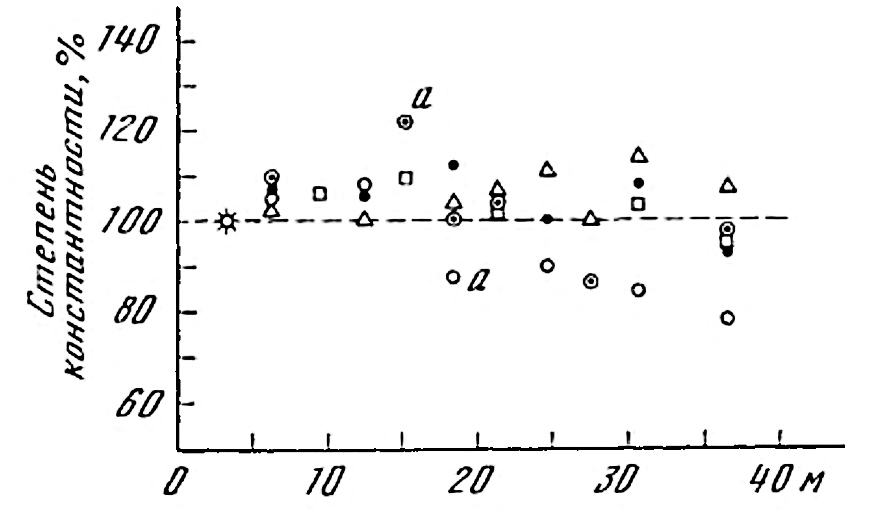
\includegraphics[width=0.65\linewidth]{figures/f5.1.png}
\end{figure}
\figblock{5.1}{Summary diagram of the Holway--Boring experiment: ratio of disc diameters
  (first/second) vs.\ distance to second disc.  Points above the dashed line correspond to
  ``superconstancy''.}

\begin{figure}[H]
    \centering
    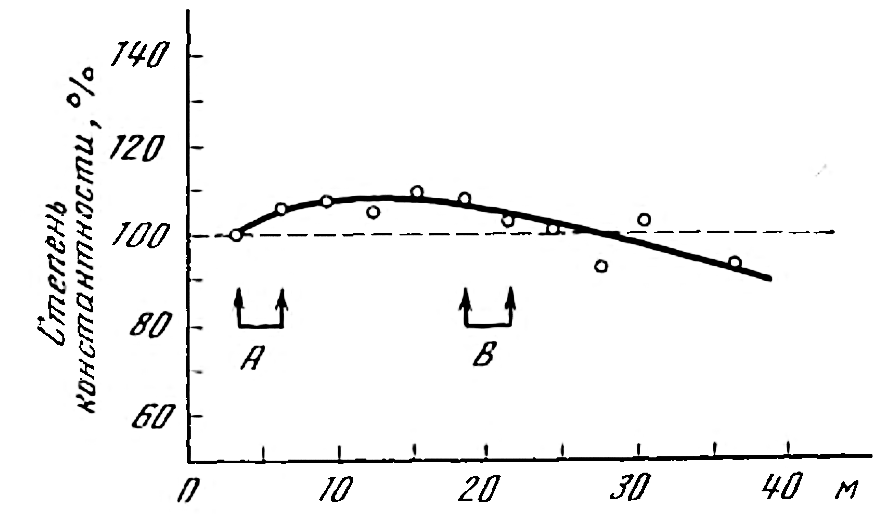
\includegraphics[width=0.65\linewidth]{figures/f5.2.png}
\end{figure}
\figblock{5.2}{Curve of mean constancy vs.\ distance, derived from Fig.\,5.1.  The maximum
  occurs at 10--15\,m.  Reverse perspective can occur only to the left of the maximum (up
  to $\sim$10\,m); to its right, widths progressively decrease.}

In those cases where the phenomenon of ``superconstancy'' was not observed in other
experiments (since the numerical values in such experiments depend strongly on experimental
methodology), the increase of constancy in the transition from monocular to binocular
vision was nonetheless firmly established.  Thus in the experiments of A.\,A.~Smirnov and
M.\,N.~Volokitina,\footnote{A.\,A.~Smirnov, M.\,N.~Volokitina.  Dependence of the
  constancy of the perceived size of objects on their mutual separation at various observation
  distances.---In: \emph{Visual Sensations and Perceptions}, Moscow--Leningrad, 1935.}
the increase of constancy in the transition from monocular to binocular vision averages
5--10\%, i.e.\ it is of the same order as in the Holway--Boring experiments.

\srcpage{261}

One should not think that the location of experimental points above the dashed line in
Fig.\,5.1 itself testifies to the emergence of the reverse-perspective effect.  To clarify
this, refer to Fig.\,5.2, which shows the curve of the arithmetic mean constancy obtained
by processing the experimental points of Fig.\,5.1.

The graph in Fig.\,5.2 shows a maximum degree of constancy in the distance range 10--15~m.
The reverse-perspective effect can be observed only to the left of the maximum, i.e.\ at
distances up to about 10~m, since the essence of reverse perspective is the increase of
lateral size with distance, while to the right of the maximum a progressive decrease in this
size will occur.  Indeed, a rectangular object of depth 3~m whose front face is 3~m from
the observer will have a visible size of its far edge 5\% larger than the front (region~$A$
in Fig.\,5.2), while if shifted to a distance of $\sim 18$~m it will be characterised by a
decrease of the visible size of the far edge relative to the front by 2\% (region~$B$ in
Fig.\,5.2).  Thus it is not the very fact of superconstancy but the \emph{increase} of the
degree of constancy with distance that is decisive for the emergence of the reverse-perspective
effect.  If one takes as a basis the data from the Holway--Boring experiments, the
``natural'' reverse-perspective effect associated with the binocularity of human vision
should be observed at distances up to 10~m.

Using the initial, steepest part of the curve shown in Fig.\,5.2, corresponding to distances
3--6~m, one can estimate the degree of expression of the reverse-perspective perception.
If these data are used to determine the visual appearance of a rectangle having an aspect
ratio of 1:3 with its long side oriented away from the observer, the calculations give the
degree of divergence of the parallel lines in visual perception as of the order of $2°$, i.e.\
the effect described here can lead to only a very weak reverse perspective.

\srcpage{262}

In Appendices~2 and~3 a mathematical description of a simplified perceptual perspective
system was given, in which the function $P_1$ was determined from conditions corresponding
to monocular vision.  To determine the function $P_1$ from the laws of binocular vision,
it suffices to modify condition~(2.3) as follows:
\begin{equation}
  \frac{dP_1}{dl}(0) = 1 + \alpha,  \tag{5.1}
\end{equation}
where $\alpha > 0$, and the quantity~$\alpha$ should be determined from experiment (e.g.\
from the experiment described in the present Appendix).

% Appendix 6: The Occurrence of Reverse Perspective When Viewing Objects in Foreshortening
% Source pages: 262–270

\chapter{The Occurrence of Reverse Perspective When Viewing Objects in Foreshortening}

\srcpage{262}

The considerations presented in the preceding Appendix testify to the possibility of genuine
vision according to the laws of reverse perspective, provided that visual perception exhibits
``superconstancy''.  The weakness of that argument lies in the fact that, according to
current experimental data, the phenomenon of ``superconstancy'' is not registered in all
people.  Mathematical analysis shows, however, that the requirement of ``superconstancy''
is not necessary.  A person whose visual perception is characterised by only full---and even
somewhat incomplete---constancy can also see in reverse perspective (the discussion, as in
the preceding Appendix, concerns only distances of the order of a few metres).  This type
of visual perception is characteristic of the vast majority of people, not only under
binocular but also under monocular vision.

The mentioned effect will be observed in those cases when the parallel strips that a person
is looking at run not directly \emph{away from} the viewer, but at a slight \emph{angle}.

To take the decisive step in the analysis, it is necessary to introduce a highly important
concept---the \emph{zero line}.  Note the well-known inequality of the ``stretchings'' of
the retinal image by the visual-perception system in the $x$ and $y$ directions.  Recall
that the region of clear vision in man is comparatively small, and in surveying the space
before him a person involuntarily shifts his gaze from one region to another.  The region
on which he is looking at a given moment then serves as a kind of ``origin'', while all
other regions of space are assessed relative to it---they may be ``closer'', ``farther'',
``to the left'', ``to the right''.  The concepts ``closer'' and ``farther'' are, in a
certain sense, absolute, while ``to the left'' and ``to the right'' are relative: their
meaning does not change under turns of the head, whereas the concepts ``left'' and
``right'' can change their meaning under such turns.

Turning to an analytical treatment, we adopt the following notation.  Coordinates
$(\bar{x}_H, l)$ correspond to the subject plane, $(x_1, y_1)$ to the linear-perspective
system, and $(x_2, y_2)$ to the perceptual-perspective system.  The absence of subscripts
on $x$ and $y$ indicates that the statements made apply equally to two or all three of the
coordinate systems.

\srcpage{263}

The size-constancy mechanism will therefore always ``stretch'' the retinal image in the
$y$-direction uniformly, regardless of where the person looks (since this axis represents
movement ``near''---``far''), with the stretchings described by relation~(2.6).  As for
the stretchings along the $x$-axis, formula~(2.1) applies, linking $x_2$ not only
with~$l$ but also with~$x_1$---the distance of the point from some axis conventionally
taken as zero.  Movement parallel to the $x$-axis represents lateral movement.

In the previous Appendices it was always assumed that the person looks straight ahead,
perpendicular to the picture plane, and that the axis of the ``path'' runs in the same
direction.  In that case the image of the axis coincided with the principal axis of the
picture, which was naturally taken as the zero line from which the distances~$x_1$ were
measured left and right.  In passing to perceptual perspective, $x_1$ was multiplied
by~$P_1(l)$ to find~$x_2$.  Only points with $x_1 = 0$ underwent no lateral shifts,
since their new abscissa $x_2 = x_1 = 0$.

We define the \textbf{zero line} as the line that undergoes no lateral shifts in the
transition from the linear-perspective system to the perceptual-perspective system.

\begin{figure}[H]
    \centering
    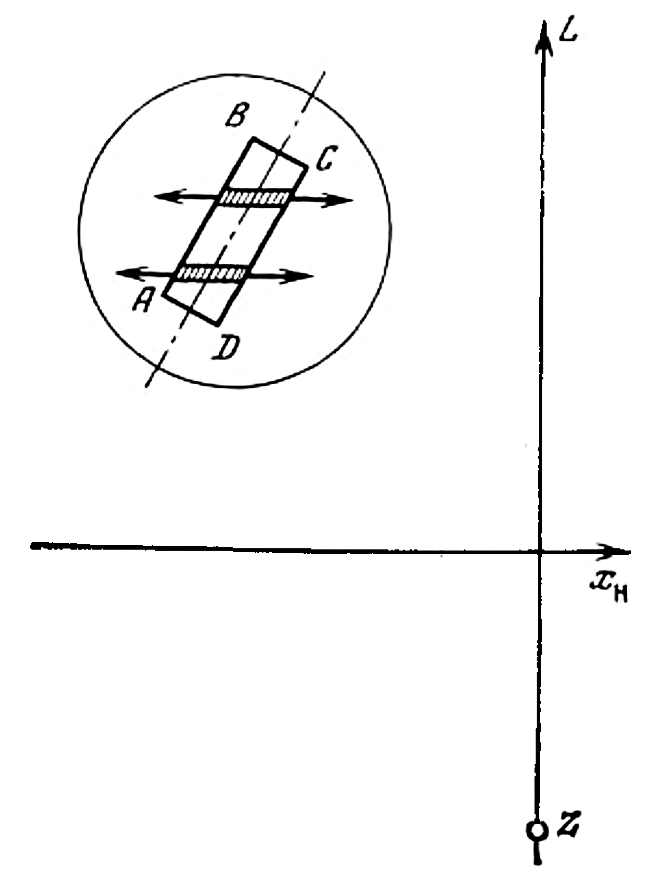
\includegraphics[width=0.4\linewidth]{figures/f6.1.png}
\end{figure}
\figblock{6.1}{Diagram of the subject plane (view from above) showing a viewer at point~1
  and a rectangle~$ABCD$ lying to one side of the depth axis.  The circle marks the region
  of clear vision.  Arrows indicate lateral ``stretchings'' away from the zero line
  (dash-dot), which is the axis of the rectangle rather than the depth axis.}

\srcpage{264}

In those cases when the sole object lies to one side of the depth axis (Fig.\,6.1), the
zero line turns out to be not the $l$-axis but the axis of rectangle $ABCD$ (dash-dot
line).  The zero line is determined by the central part of the retinal region of clear
vision; the stretchings proceed from it ``outward''.  It is not perpendicular to the
picture base but is inclined at an angle depending on the position of $ABCD$ on the
subject plane.

\begin{figure}[H]
    \centering
    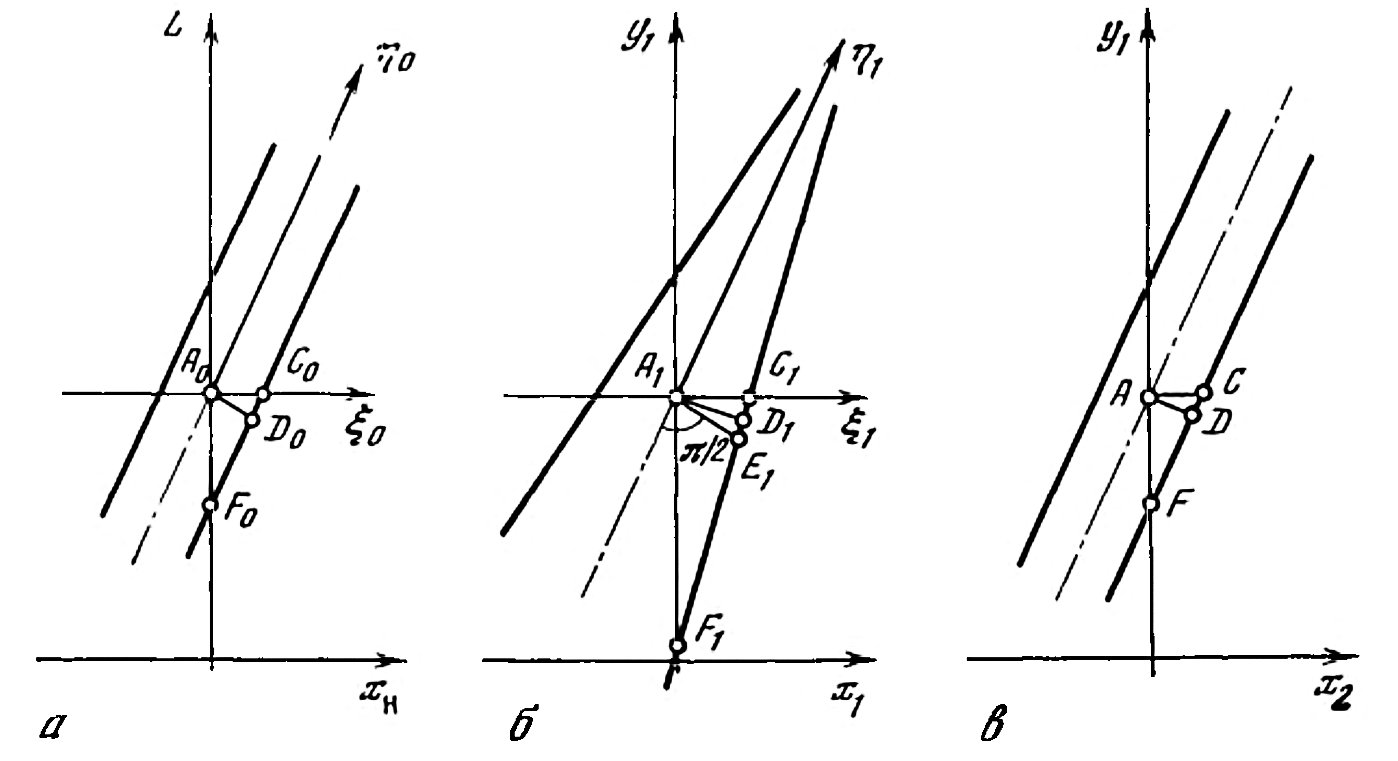
\includegraphics[width=1.0\linewidth]{figures/f6.2.png}
\end{figure}
\figblock{6.2}{Three-part scheme: (a)~subject plane with two parallel lines and the zero
  line; (b)~image in linear perspective; (c)~mixed coordinate image $(x_2, y_1)$
  showing the axis and near edge as parallel straight lines.}

For simplicity, we replace the elongated rectangle by a strip with parallel edges and
assume full constancy for near objects (not an obligatory assumption, as discussed below).
Our immediate aim is only the \emph{qualitative} proof that reverse-perspective perception
arises when contemplating a strip with parallel edges directed ``obliquely''.

Fig.\,6.2,\,a shows the subject plane (view from above) with two parallel lines [bars
over variable names indicate dimensionless notation according to formulas~(1.1)]:
\begin{align}
  \bar{l}^{**} &= \bar{a}_0'' + \bar{b}_0\,\bar{x}_H,  \tag{6.1a}\\
  \bar{l}^{*} &= \bar{a}_0' + \bar{b}_0\,\bar{x}_H.   \tag{6.1b}
\end{align}
($\bar{l}^{**}$ is the left, $\bar{l}^*$ the right line.)  We assume these lines to be
close together and that both pass (on the interval of~$\bar{x}_H$ under consideration)
near the picture plane, so that $l$ is small for all considered points.  The equation of
the axial line of the strip is
\begin{equation}
  \bar{l}_0^0 = \bar{a}_0^0 + b_0\,\bar{x}_H.  \tag{6.2}
\end{equation}
The smallness of~$l$ permits the assumption of full constancy, which requires choosing the
function $P_1$ in the form
\begin{equation}
  P_1(l) = 1 + l.  \tag{6.3}
\end{equation}

\srcpage{265}

Fig.\,6.2,\,b shows the image of the strip in linear perspective.  The equation of the
axial line in this system is
\begin{equation}
  y_1^0 = a_1^0 + b_1\,\hat{x}_1, \qquad
  a_1^0 = \frac{a_0^0}{1+a_0^0},\quad b_1 = \frac{b_0}{1+a_0^0}.  \tag{6.4}
\end{equation}

To describe the ``stretching'' of the retinal image using the zero-line concept, we
introduce an oblique coordinate system $(\xi_0, \eta_0)$ in the subject plane so that the
$\eta_0$-axis coincides with the zero line and the $\xi_0$-axis is parallel to~$\bar{x}_H$
(Fig.\,6.2,\,a).  The axial line has equation $\xi_0 = 0$ by definition, and the strip
edges have equations $\xi_0 = -c$ and $\xi_0 = c$, where $c$ is a constant.  On passing
to linear perspective, the oblique coordinate transforms as
\begin{equation}
  \xi_1 = \frac{\xi_0}{1 + l},  \tag{6.5}
\end{equation}
so that the right edge of the strip becomes
\begin{equation}
  \xi_1^* = \frac{c}{1+l}.  \tag{6.6}
\end{equation}

When the visual-perception system forms the perceptual space, $\xi_1^*$ is ``stretched''
[formula~(2.1)]: $\hat\xi_2^* = \xi_1^*\,P_1(l)$, whence, using~(6.3) and~(6.6),
\begin{equation}
  \hat\xi_2^* = \hat\xi_1^* P_1(l)  = c.  \tag{6.7}
\end{equation}

\srcpage{266}

We build the image of the strip in the auxiliary \emph{mixed} coordinate system $(x_2, y_1)$.
Since points of the zero line undergo no lateral shifts in passing from $(x_1, y_1)$ to
$(x_2, y_2)$, the equation of the zero line in the mixed system is the same as in
$(x_1, y_1)$:
\begin{equation}
  y_1^0 = a_1^0 + b_1\,\bar{x}_2.  \tag{6.8}
\end{equation}
For the near (lower in the schemes) edge, since $x_2 = x_1 + c$,
\begin{equation}
  y_1^* = a_1^* + b_1\,\bar{x}_2, \qquad a_1^* = a_1 - b_1\,c.  \tag{6.9}
\end{equation}
Comparing~(6.8) and~(6.9) shows that in the mixed system the axial line and the near edge
have become \emph{parallel} straight lines (see Fig.\,6.2,\,c).

To pass to the perceptual-perspective system one accounts for the $y$-direction stretching.
Since this stretching proceeds according to relation~(2.6), in which $x$-coordinates do
not appear, both lines transform identically:
\begin{equation}
  dy_2 = P_1(l)\,dy_1.  \tag{6.10}
\end{equation}
Using~(6.3) together with~(6.10) and equations~(6.8)--(6.9), one obtains
\begin{equation}
  \frac{dy_2^{\,\text{axis}}}{dx_2} = b_1(1+l_A),\qquad
  \frac{dy_2^{\,\text{near}}}{dx_2} = b_1(1+l_B).  \tag{6.11}
\end{equation}

These expressions determine the slopes of the tangent lines relative to the $x_2$-axis.
Since the $x$-coordinates do not appear in~(6.11), for simplicity consider the region near
the $y$-axis.  For all points lying below~$C_0$ on the near edge, the values of~$l$
are smaller than at point~$A_0$ on the axis (e.g.\ $l_B < l_A$), since the strips
are inclined with~$b_0 > 0$.  This gives the inequality

\srcpage{267}

\begin{equation}
  \left.\frac{dy_2^0}{dx_2}\right|_A > \left.\frac{dy_2^*}{dx_2}\right|_D,  \tag{6.12}
\end{equation}
which says that in perceptual space objectively parallel lines are seen as diverging with
increasing depth---the axial line appears steeper than the near edge.  \emph{This is the
reverse perspective.}  As is clear from the argument, the conclusion is unchanged if one
compares point~$A_0$ with~$E_0$, or with a point lying on the perpendicular to the
perceptual-perspective image of the axial line.

Consequently, when viewing near, narrow strips with objectively parallel edges arranged
``obliquely'', a person sees them in reverse perspective.  Thus reverse perspective is a
\emph{norm} of human vision at short distances.  The present considerations indicate a
method by which a modern person too can see space in reverse perspective; it is described
in Chapter~V.

\begin{figure}[H]
    \centering
    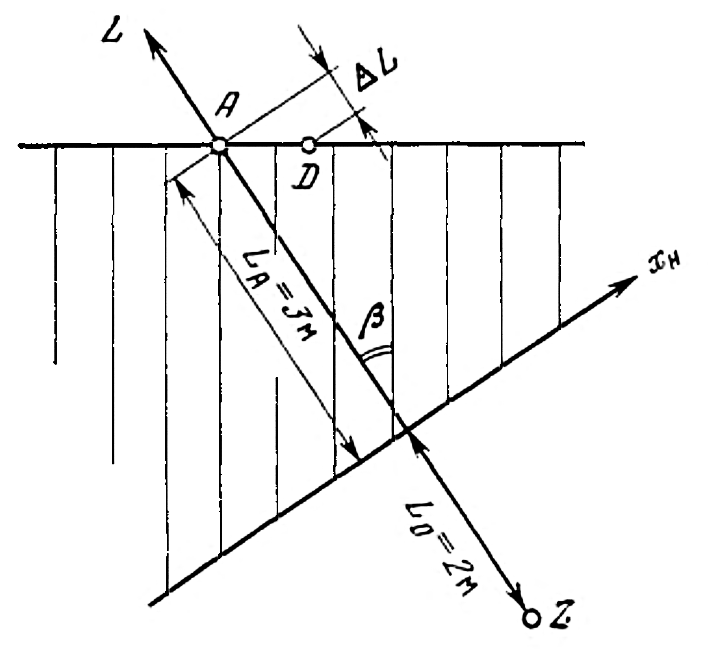
\includegraphics[width=0.6\linewidth]{figures/f6.3.png}
\end{figure}
\figblock{6.3}{Plan of a room with parquet strips of width~$B$.  The viewer stands at
  point~$I$ and looks in the direction making angle~$\beta$ with the strip structure.
  The far wall $AD$ is 5\,m away.}

Although the derivations above were intended to give only a qualitative proof, the
obtained expressions permit quantitative estimates.  Consider the example of observing the
parallel structure of a floor.  Fig.\,6.3 shows a plan of a room with parquet strips of
width~$B$; the viewer stands at point~$I$ and looks in a direction making angle~$\beta$
with the linear structure of the floor.  The far wall is 5\,m from the viewer.

\srcpage{268}

We estimate the angular divergence of a group of parallel parquet strips in the region of
the far wall.  The angle~$\beta$ is chosen to give the maximum divergence effect.

Using formulas~(1.1) and the results of the present Appendix,
\begin{equation}
  \frac{dy_2}{dx_2} = \frac{Hb_1(1+l/l_0)^2}{B},  \tag{6.13}
\end{equation}
where
\begin{equation}
  b_1 = \frac{b_0}{1+a_0},\quad a_0 = \frac{a}{b_0},\quad l_0 = \frac{bB}{l_0}.
  \tag{6.14}
\end{equation}
(It should be remembered that $b_1$ is computed at point~$A$.)

The angle of non-parallelism of the strip boundaries at points $A$ and $D$ in visual
perception is
\begin{equation}
  \alpha = \arctan\!\left.\frac{dy_2}{dx_2}\right|_A
         - \arctan\!\left.\frac{dy_2}{dx_2}\right|_D  \tag{}
\end{equation}
Assuming the depths of $A$ and $D$ to be close and writing $l_D = l_A - \Delta l$
($\Delta l$ small), one obtains the approximate formula
\begin{equation}
  \alpha = \frac{d}{dl}
         \arctan\!\left.\frac{dy_2}{dx_2}\right|_A \Delta l  \tag{6.15}
\end{equation}
\begin{equation}
  \alpha \approx \frac{\Delta l \ b_1\,H/Bl_0}
    {1 + \bigl[b_1\,H(1+l_A/l_0)/B\bigr]^2}.  \tag{6.16}
\end{equation}

Setting $d\alpha/db_1 = 0$ to maximise~$\alpha$ with respect to the direction of gaze,
\begin{equation}
  b_1^{\,*} = \frac{B}{H(1+l_A)};  \tag{6.17}
\end{equation}
here and below asterisks mark quantities giving the maximum of~$\alpha$.  The
corresponding optimal slope $b^*$ (determining the angle $\beta^*$ in Fig.\,6.3) is
\begin{equation}
  b^* = \frac{l_0}{H}.  \tag{6.18}
\end{equation}
Substituting~(6.17) into~(6.16):
\begin{equation}
  \alpha^* = \frac{\Delta l}{2(l_0 + l_A/l_0)}.  \tag{6.19}
\end{equation}

\srcpage{269}

Formulas~(6.18) and~(6.19) give the optimal direction of gaze and the expected angular
divergence of objectively parallel strips (in radians).

A noteworthy result is that both quantities are independent of~$B$.  In the present
example $b^* \approx 1.25$, i.e.\ $\beta^* \approx 39°$.  To compute~$\alpha^*$ one
must specify~$\Delta l$.  Following Fig.\,6.3, $\Delta l = AD\sin\beta^*$, showing the
natural growth of~$\alpha^*$ with increasing strip width.  Taking as a reasonable
value $\Delta H = 1.5$\,m fitting within the zone of clear vision, one immediately
obtains $\alpha^* \approx 6°$.  Thus the probable magnitude of the visible angular
divergence of objectively parallel strips amounts to several degrees and can hardly
exceed~$10°$.

\begin{figure}[H]
    \centering
    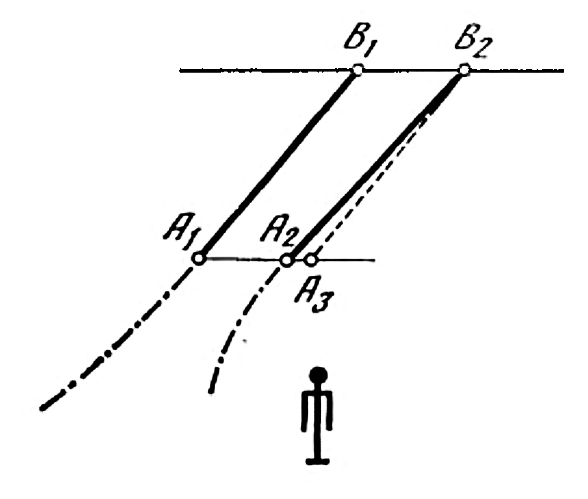
\includegraphics[width=0.45\linewidth]{figures/f6.4.png}
\end{figure}
\figblock{6.4}{Results of the author's experiments.  Objectively parallel lines viewed
  obliquely at $20°$--$30°$ and fixated at 4--6\,m appear to diverge from~$A_1A_2$ to
  the far wall~$B_1B_2$.  Closer to the observer the same lines appear to converge
  (dashed lines), since the peripheral visual field is aconstant.}

The numerical estimates obtained here agree well with the experimental data cited below,
and this is all the more remarkable since no experimental constants were employed in the
derivation.  In essence, both the qualitative and quantitative results rest on only two
assumptions: the hypothesis of the existence of a zero line, and the condition that at
short distances human vision is characterised by full constancy.

The last assumption can be substantially relaxed.  Since the resulting reverse perspective
is sufficiently large, it may be assumed that visual perception exhibits incomplete
constancy.  For example, if under full constancy reverse perspective amounts to about~$5°$,
and if due to incomplete constancy the observer perceives the parallel edges of a strip
seen along their length as slightly converging (with a convergence angle of~$3°$--$4°$),
it is not difficult to see that when looking at them ``obliquely'' he can perceive a weak
reverse perspective of~$1°$--$2°$.

\srcpage{270}

Let us examine some experimental data confirming the above propositions.

As far as the author is aware, the first to describe genuine vision in reverse perspective
was A.~Bakushinsky.\footnote{See: \emph{Iskusstvo}, 1923, No.\,1, p.\,235.}  Having
developed his own, somewhat erroneous, theory (see Ch.\,IV), he was psychologically
prepared to see objects in reverse perspective, and he actually did so.  Here is his
description: ``\ldots the perception of books of the same format and size, scattered on
the floor in depth from the viewer\ldots The impression will be as follows: the visible
rectangles, increasing in their sizes in reverse perspective up to a certain point in
depth, will thereafter diminish and foreshorten in normal perspective.''  Unfortunately,
Bakushinsky gave no numerical data connected with his observations, and his remark that
one can see city roofs in reverse perspective from a bell-tower arouses doubt (this is
probably an armchair conclusion).

The experiments carried out by the author consisted in observing clear and manifestly
parallel lines (edges of a carpet runner, parquet strips, large rectangular floor
patterns, etc.) by the method of Appendix~3 (see Fig.\,3.2).  The width of the
formations ranged from 0.5 to~1.2\,m and the depth from 5 to~8\,m.  Observations were
made indoors, sitting and standing.  The reverse-perspective effect was observed when
contemplating parallel lines ``receding'' from the viewer if they lay somewhat to one
side ($20°$--$30°$ in the described experiments) and when the gaze was fixed on a
section 4--6\,m from the viewer.  Objectively parallel lines appeared slightly diverging
(Fig.\,6.4), from a certain distance~$A_1A_2$ up to the far wall~$B_1B_2$.  Measurement
gave a point~$A_3$ to the right of~$A_2$ when a line parallel to~$A_1B_1$ was
constructed from~$B_2$ by the ruler method.  The distance~$A_2A_3$ amounted to
approximately 5--10\% of~$A_1A_2$, corresponding to a divergence angle of about
$2°$--$3°$.  When the gaze was fixed on the far part of the parallel lines, the near
section (closer than~$A_1A_2$) appeared to converge in depth---obeying normal
perspective (dash-dot lines in Fig.\,6.4).  This is connected with the aconstancy of
peripheral vision: in the peripheral visual field an image close to the retinal image
arises.

% Appendix 7: Reverse Perspective and Lobachevsky Geometry
% Source pages: 270–274

\chapter{Reverse Perspective and Lobachevsky Geometry}

\srcpage{270}

As is well known, objective external space (meaning the objects with which the artist
deals) may be considered Euclidean.  In the process of transforming this space into
perceptual space it undergoes substantial deformations, so that its geometry is not obvious.

In 1947, Luneburg showed that in its properties perceptual space may be considered a
space of Lobachevsky.\footnote{A brief account of Luneburg's work and bibliography: see
  S.~Koch (Ed.).\ \emph{Psychology: A Study of a Science}, vol.\,I\@. New York, 1959.}
Luneburg based this conclusion on the well-known experiments of
Blumenfeld,\footnote{W.~Blumenfeld.  Untersuchungen \"uber die scheinbare Gr\"o\ss e im
  Sehraume.---\emph{Z.~Psychol.~Physiol.~Sinnesorgane}, 1913, 65, S.\,241.}
in which it was established that if a subject observing two rows of points on a horizontal
plane is asked first to arrange the points so that the rows appear \emph{parallel}, and
then to arrange them so that the distance between them appears \emph{constant}, the subject
places the points differently in the two experiments.  In Euclidean space, parallel lines
and everywhere-equidistant lines should coincide, so the discrepancy recorded by Blumenfeld
may be interpreted as indicating that perceptual space is non-Euclidean.  Both the
Blumenfeld experiments and a series of special experiments carried out to confirm Luneburg's
theory showed that for sections of a horizontal plane in the immediate vicinity of the
observer, the properties of perceptual space can indeed be described as properties of
Lobachevsky space.

In accordance with the experimental limitations existing at the present time, we consider
only the problem of transforming by the human perceptual system the retinal image of a
section of a horizontal plane of comparatively small extent.

\srcpage{271}

\begin{figure}[H]
    \centering
    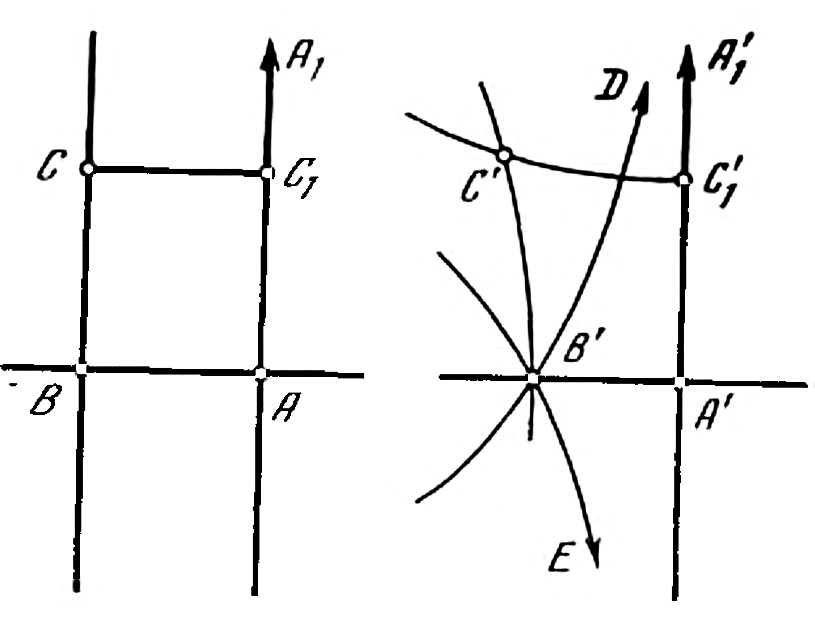
\includegraphics[width=0.55\linewidth]{figures/f7.1.png}
\end{figure}
\figblock{7.1}{Diagram (view from above) of the experiment in objective space (right
  half) and perceptual space (left half).  Objective rectangle $ABCC_1$ (with a right
  angle at each vertex) corresponds to Lambert quadrilateral $A'B'C'C_1'$ (with right
  angles at $A'$, $B'$, $C_1'$ only) in perceptual Lobachevsky space.  The far side
  $C'C_1' = k$ exceeds the near side $A'B' = a$, giving reverse perspective.}

Let the observer stand at point~$A$ in objective space on a flat horizontal patch, looking
in direction~$AA_1$ (Fig.\,7.1).  Draw $AB$ perpendicular to $AA_1$, directed along the
observer's shoulder line.  Through~$B$ draw $BC$ parallel to~$AA_1$ (in Euclidean space
this can be done in a unique way).  Drop a perpendicular from~$C$ to~$AA_1$; the result is
rectangle~$ABCC_1$.

Consider the configuration of this rectangle in perceptual space, making the natural
assumption that straight lines of objective space correspond to straight lines of perceptual
space.\footnote{This assumption, which underlies the subsequent reasoning, amounts to
  supposing that the line joining two points of perceptual space by the shortest path is
  the image of the line joining the corresponding points of objective space by the shortest
  path.  Such an assumption is sufficiently natural and biologically reasonable, since
  correct assessment of shortest distances is essential from a biological standpoint, and
  both humans and animals are guided in their behaviour by the images arising in perceptual
  space.}
Let point~$A$ correspond to point~$A'$ in perceptual space, and line~$AA_1$ to
line~$A'A_1'$.  By the symmetry that must hold between the left and right half-planes in
the observer's consciousness, line~$A'A_1'$ cannot curve in perceptual space.  Lay off
from~$A'$ the segment~$A'B'$, perpendicular to~$A'A_1'$, corresponding to segment~$AB$ of
objective space.  The line $A'B'$ is also straight in the observer's mind, since he must
perceive the upper and lower half-planes as symmetric.  Continue the construction as in
objective space.  If one starts from the experimental fact that perceptual space is a
Lobachevsky space, then through point~$B'$ one can draw \emph{two} parallels to~$A'A_1'$,
namely~$B'D$ and~$B'E$, and in addition all the infinitely many Lobachevsky lines lying
between $B'D$ and $B'E$ will also never intersect~$A'A_1'$.  Instead of the unique
line~$BC$ that does not meet~$AA_1$, the construction has thus produced infinitely many.

\srcpage{272}

To select from this family the unique Lobachevsky line corresponding to $BC$ in objective
space, one can use neither the notion of parallelism (non-intersection with~$A'A_1'$, a
property shared by the whole family) nor the notion of equidistance (no member of the
family is equidistant from~$A'A_1'$ in the Lobachevsky metric).\footnote{Were one to
  construct the line through~$B'$ equidistant from~$A'A_1'$, it would, as is well known,
  not be a straight line in Lobachevsky geometry.}  The way out is to use the mirror
symmetry of the upper and lower half-planes in the diagram of objective space.

Indeed, $AB$ may be regarded as an axis of symmetry.  Requiring the Lobachevsky line
through~$B'$ to be symmetric with respect to~$A'B'$ singles out from the family a unique
line~$B'C'$, which by that symmetry property must intersect~$A'B'$ at right angles.  Take
on~$B'C'$ the point~$C'$ corresponding to~$C$ in objective space, and drop a perpendicular
from~$C'$ to~$A'A_1'$.  The resulting quadrilateral~$A'B'C'C_1'$ corresponds to
rectangle~$ABCC_1$ of objective space.\footnote{The correspondence obtained is not only
  formally mathematical; it is conditioned in particular by the fact that in the method of
  construction adopted, the possibilities of human psychology are taken into account.
  Indeed, the right angle at vertex~$A'$ can be constructed because that vertex corresponds
  to the point where the observer stands, and the right angles at~$B'$ and~$C_1'$ can be
  constructed because foreshortening does not distort the visible magnitudes of the angles
  at~$B$ and~$C_1$.}
The quadrilateral~$A'B'C'C_1'$ has three right angles---at~$B'$ by symmetry, and at~$A'$
and~$C_1'$ by construction.  Such a quadrilateral is sometimes called a \emph{Lambert
quadrilateral}.  For a Lambert quadrilateral there is a well-known relation connecting the
sides $a$ and $b$ enclosed between the right angles with the side~$k$ opposite to~$a$
(in Fig.\,7.1: $a = A'B'$, \, $b = A'C_1'$, \, $h = C'C_1'$):
\begin{equation}
  \cos\Pi(a) = \cos\Pi(h)\,\sin\Pi(b),  \tag{7.1}
\end{equation}
where $\Pi(x)$ is the Lobachevsky function (angle of parallelism), defined by
\begin{equation}
  \Pi(x) = 2\arctan e^{-x/R}.  \tag{7.2}
\end{equation}
Here $R$ is the curvature radius of the Lobachevsky space.

\srcpage{273}

From relation~(7.1), noting that $\Pi(x) < \pi/2$ for $x > 0$, it follows that
$\sin\Pi(b) < 1$, and consequently $\cos\Pi(h) > \cos\Pi(a)$.  Since $\Pi(x)$ is a
decreasing function, this gives
\[
  k > a,
\]
i.e.\ in perceptual space the far side of the quadrilateral exceeds the near side.
\emph{This is the reverse perspective.}

Turning to everyday human experience, several facts suggest that the Lobachevskian
properties of perceptual space are characteristic only of a comparatively small region
surrounding the observer, while more distant regions must be described by Riemannian
geometry of positive curvature.  This is indicated by the familiar fact of spatial visual
perception---all objectively parallel lines are perceived as converging to a point on the
horizon.  Since everyday experience leads one to suppose that distant regions of perceptual
space have positive curvature, while the experiments connected with Luneburg's theory show
that the immediately surrounding perceptual space has negative curvature, one may conjecture
that the curvature of perceptual space is \emph{variable}.  The corresponding Riemannian
space model must therefore have some positive curvature at large distances from the
observer, gradually diminishing as one approaches him, and becoming negative in his
immediate vicinity (under binocular vision).

Without aiming to specify here the only-sketched properties of the Riemannian space of
variable curvature, we note only that the geometry of perceptual space is in fact even more
complex.  The closest analogy of perceptual space is \emph{Einstein space}.  In Einstein's
general theory of relativity, space has variable curvature depending on the masses
contained in it.  Recall, however, that at the end of Chapter~III, when discussing
Ill.\,26, it was shown that the geometric properties of perceptual space depend on the
objects depicted in it.  In this connection, if one speaks of an analogy between Einstein
space and perceptual space, then in the latter, \emph{a priori} information plays a role
analogous to that of mass in general relativity: just as an increase of mass in some region
of physical space increases its curvature, an increase of a priori information about the
objects in some region of perceptual space increases its deformation.

\srcpage{274}

All the questions touched upon here are still entirely undeveloped and can be advanced only
through the mathematical processing and interpretation of a series of carefully designed
experiments.

% Appendix 8: The Rigid System of Perceptual Perspective
% Source pages: 274–281

\chapter{The Rigid System of Perceptual Perspective}

\srcpage{274}

To construct the rigid system of perceptual perspective, one must solve the problem of
depicting an individual point of picture-space on the picture plane, and obtain a
\emph{unique} solution.  Any point of picture-space must always be depicted by the same
point of the picture plane, regardless of how the corresponding constructions are carried
out.  In addition, one must require that the construction correspond as fully as possible
to natural visual perception.

As proved in Appendix~2, a perfect transmission of the geometry of visual perception on
the picture plane is in principle impossible, which, when applied to depicting an
individual point, means the impossibility of adequately transmitting all three of its
coordinates.  The artist's freedom of choice in the perceptual perspective system
consists, as already mentioned, in deciding which one of the three coordinates to transmit
with distortion, and which ones without.  One must then verify that this choice leads to a
reasonable method of construction on the picture plane.

Since the system to be built should best serve \emph{landscape} painting, in which large
numbers of prominent verticals are absent, we attempt to construct the system by tolerating
distortion in the less significant vertical dimensions.

\srcpage{275}

We formulate the following requirements for the rigid perceptual perspective system under
consideration.  Let the \emph{module} (the unit of linear size) be the depicted length of
a horizontal segment parallel to the picture plane situated on the middle ground at
distance~$l_*$ from the picture plane.  We require that the scales of depiction of
analogous segments on the near and far grounds be consistent with visual perception (relative
to the module), and that the same property hold for all other horizontal segments on all
three grounds; on the far ground we additionally require the same scale consistency for
vertical segments.  Thus, only the vertical dimensions on the middle and near grounds will
be distorted.

To give these general considerations concrete form, we turn to a rigorous formulation of
the problem.

Introduce the linear-perspective and perceptual-perspective coordinate systems with
coordinates $(x_1, y_1)$ and $(x_2, y_2)$ respectively.  A line lying in the subject
plane, perpendicular to the picture plane, and passing through the observer's position,
is naturally taken as the $y_1$-axis (equation $x_1 = 0$); the same position is adopted
for the $y_2$-axis.

If one mentally traces on the subject plane the lines of equal~$l$ and lines perpendicular
to them (forming a coordinate grid), then on the image the lines of equal~$l$ correspond
to horizontal lines, and the perpendicular family corresponds to a series of lines passing
through the principal point of the picture (straight lines in linear perspective, curves in
perceptual perspective).  Each point of the subject plane is thus represented by a unique
point on the image.

To obtain the image of points of picture-space, one must agree on how vertical segments
of picture-space are to be depicted.  Let them also be vertical on the picture plane.
This is a natural requirement, since the picture plane is perpendicular to the subject
plane.  The question of \emph{how large} to make the depiction of a vertical segment turns
out to be more complex.  Along the $y_2$-axis are laid off both images of vertical
segments \emph{and} segments conveying the recession from the picture plane; these must be
reconciled.  Let a vertical object of height~$H$ stand in the picture plane; its top then
projects on the horizon line.  However, the distance from the base of the picture to the
image of the horizon line exceeds this height: in Appendix~3 it turned out to equal
$(1+\pi/4)H$.  Since by hypothesis distortions are to be shifted onto the vertical
dimensions, the object of height~$H$ must be depicted as having size $(1+\pi/4)H$ in
order that its top also falls on the horizon line.

\srcpage{276}

Suppose the top of every object of height~$H$, wherever it stands in picture-space, must
project onto the horizon line.  Then an object of height~$H$ at depth~$l$ must be shown
with image height~$H_2$ satisfying, on the basis of formulas~(1.1) and~(2.6),
\begin{equation*}
  H \int_{0}^{\infty} \frac{P_1(l)}{(1+l)^2}\,dl + H_2
  = H \int_{0}^{l} \frac{P_1(t)}{(1+t)^2}\,dl + H_2 \, .
\end{equation*}
Hence
\begin{equation*}
  H_2 = H\int_{l}^{\infty} \frac{P_1(l)}{(1+l)^2}\,dl.
\end{equation*}
Extending this condition to all other vertical segments, an object of height~$z$ at
depth~$l_B$ is depicted with size
\begin{equation}
  h_2 = z\int_{l_B}^{\infty} \frac{P_1(l)}{(1+l)^2}\,dl.  \tag{8.1}
\end{equation}

We assess the degree of distortion of heights under this method of depiction.  The
visually perceived size of height~$z$ is determined by formulas~(1.3) and~(2.1):
\begin{equation}
  h_2^* = z\,\frac{P_1(l_B)}{1+l_B}.  \tag{8.2}
\end{equation}
Denote by~$\varepsilon$ the ratio of the depicted size of height~$z$ to its visually
perceived size:
\begin{equation}
  \varepsilon = (1+l_B)\displaystyle\int_{l_B}^{\infty}
    \frac{P_1(l)}{(1+l)^2}\,dl \ [P_1(l_B)]^{-1}.  \tag{8.3}
\end{equation}
Using the specific dependence $P_1(l_B) = 1 + \arctan l_B$, the relation between $\varepsilon$
and~$l_B$ can be represented as a graph (Fig.\,8.1), whose general character is unchanged
for other specific forms of~$P_1$.

\begin{figure}[H]
    \centering
    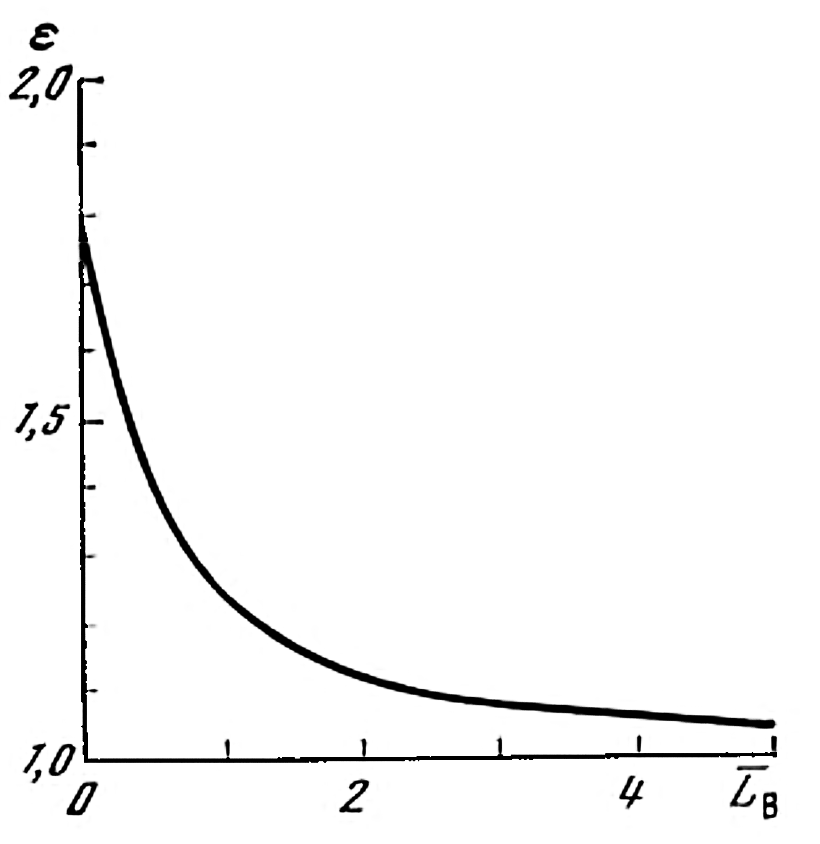
\includegraphics[width=0.4\linewidth]{figures/f8.1.png}
\end{figure}
\figblock{8.1}{Graph of the distortion factor~$\varepsilon$ (ratio of depicted height to
  visually perceived height) as a function of depth~$l_B$.  The distortion is significant
  only for the nearest zone; from $l_B \approx 4$ onward $\varepsilon \approx 1$, and
  exactly $\varepsilon = 1$ as $l_B \to \infty$.}

\srcpage{277}

This graph conveys one extremely important circumstance: the chosen type of distortion,
characterised by~$\varepsilon$ (its deviation from unity), is significant only for the
nearest regions of space.  Beginning from $l_B \approx 1$, the value of~$\varepsilon$
exceeds unity by only about 20\% in the case under consideration, and after $l_B \approx 4$
it may be approximately taken as unity.  The exact value $\varepsilon = 1$ is attained
only as $l_B \to \infty$.  Consequently, if depicting a landscape that has no tall objects
in the foreground, these formally existing distortions cannot manifest themselves.

We now introduce the functions
\begin{align}
  P_2(l) &= \frac{P_1(l)}{1+l},  \tag{def.}\\
  P_3(l) &= \int_0^{l} \frac{P_1(l)}{(1+l)^2}\,dl,  \tag{def.}
\end{align}
so that $P_3(\infty) = \int_0^\infty P_1(t)/(1+t)^2\,dt$.  We give a summary of the
final formulas describing the variant of the rigid perceptual perspective system discussed.

Let $b$, $X$, $z$ be the coordinates of some point in picture-space, where $z$ is the
height above the subject plane and $X$ is the lateral coordinate.  Let the corresponding
quantities in the picture plane be $y_2$, $x_2$, $h_2$.  Then
\begin{equation}
  y_2 = H\,P_3(l),\quad
  x_2 = X\,P_2(l),\quad
  h_2 = z\bigl[P_3(\infty) - P_3(l)\bigr].  \tag{8.4}
\end{equation}

If the module is taken as the image of a horizontal segment parallel to the picture plane,
situated at distance~$l_*$, and for simplicity numerically equal to the eye height~$H$,
the formulas become
\begin{equation}
  \tilde{y}_2 = M\,\frac{P_3(l)}{P_2(l_*)},\quad
  \tilde{x}_2 = \frac{MX\,P_2(l)}{H\,P_2(l_*)},\quad
  \tilde{h}_2 = \frac{M z \ P_3(\infty) - P_3(l)}{H \ P_2(l_*)},  \tag{8.5}
\end{equation}
where $M$ is the dimensional unit magnitude depending on the size of the picture.  If
it is desired to measure $y_2$ from the lower edge of the picture corresponding to
$l = l_k$,
\begin{equation}
  \tilde{y}_2 = M\,\frac{P_3(l) - P_3(l_k)}{P_2(l_*)}.  \tag{8.6}
\end{equation}

The constructed perspective system possesses the important property of
\emph{commutativity}.  This property means that the ``transition'' from some point~$A$
to another point~$B$, decomposed into elementary movements ``away'', ``toward'',
``sideways'', and ``upward'', is independent of the order of these elementary movements.
If one wished to transmit vertical segments also in their visually perceived magnitudes,
the commutativity property would be violated.  Indeed, let one need to pass from
point~$A$ with coordinates $(l = X = z = 0)$ to point~$B$ with
$(l = l_B,\; X = 0,\; z = H_1)$.  Moving first horizontally then vertically,
the distance of the depicted point~$B$ from the picture base is
\[
  HP_3(l_B) + H_1\bigl[P_3(\infty) - P_3(l_B)\bigr];
\]
reversing the order gives the same expression identically.  If, however, the height~$H_1$
is depicted by its visually perceived size
\[
  h^* = H_1\,P_2(l),
\]
then depending on the order of movements the distance turns out to be either
\[
  HP_3(l_B) + H_1P_2(l_B)
\]
or
\[
  H_1 + (H - H_1)P_3(l_B),
\]
which are in general different.\footnote{It is easy to verify that ordinary linear
  perspective possesses the commutativity property.}

\srcpage{278}

Following visual perception thus leads to discontinuities in the image.  Therefore the
``primacy of continuity'' discussed in Chapter~V has a precise mathematical meaning: it
is the fulfilment of the commutativity conditions.

Consider now the case in which the distortions are shifted entirely onto $y_2$, while
$H_2$ and $x_2$ are both to be transmitted without distortion.  Then instead of~(8.4),
\begin{equation}
  x_2 = X\,P_2(l),\quad
  H_2 = z\,P_2(l),\quad
  y_2 = H\bigl[1 - P_2(l)\bigr].  \tag{8.7}
\end{equation}
As was shown above, requiring $H_2$ and $y_2$ to be simultaneously undistorted violates
commutativity.  Thus this variant of the rigid perceptual perspective system does not exist.

This circumstance prompts closer examination of the problem of conveying depth.  All
textbooks on the psychology of visual perception state that the remoteness of a point on
the ground surface may be judged by how close it is to the horizon line in the visual field;
for this reason it was assumed throughout that the depth of a point from the observer is
characterised by the coordinate~$y_2$.  There is, however, an analogous depth indicator---
probably much weaker, but not to be ignored entirely.  Imagine looking along the axis of a
long corridor: the remoteness can be judged not only from the height of a point in the
visual field but also from its horizontal position relative to the walls.  Lowering the
viewpoint to floor level makes this clearest: all $y_2 = 0$, yet the sense of depth does
not vanish.  This permits conveying depth using not only vertical but also horizontal
displacement.  A new coordinate~$\xi$ could be introduced along the $x_2$-axis, measured
from the vertical plane through the principal point.  This situation will not be developed
further here, since such effects are much weaker than the principal effect associated
with~$y_2$, and play a subordinate role in visual perception.

\srcpage{279}

The possibility of shifting the inevitable distortions in various ways allows variants of
perceptual perspective systems to be developed in which these distortions are not
concentrated on one coordinate but distributed among them, in order to seek in this way
optimal systems in some sense.  Such a problem is not considered in the present work.

In conclusion, we clarify the comparative assessments of the two perspective systems given
in the table of Chapter~X.  We give the necessary summary of formulas.

Natural visual perception is described by
\begin{equation}
  x_2^* = X\,P_2(l),\quad y_2^* = H\,P_3(l),\quad h_2^* = z\,P_2(l),  \tag{8.8}
\end{equation}
and the variant of the perceptual perspective system discussed in detail above by
\begin{equation}
  x_2 = x_2^*,\quad y_2 = y_2^*,\quad
  h_2 = z\bigl[P_3(\infty) - P_3(l)\bigr].  \tag{8.9}
\end{equation}
As for the linear perspective system, it is obtained from~(8.8) or~(8.9) by setting
$P_1 \equiv 1$, which gives $P_2(l) = 1/(1+l)$, $P_3(l) = l/(1+l)$, $P_3(\infty) = 1$:
\begin{equation}
  x_1 = \frac{X}{1+l},\quad y_1 = \frac{Hl}{1+l},\quad h_1 = \frac{z}{1+l}.  \tag{8.10}
\end{equation}

In compiling the comparison table, the condition was adopted that the size~$a$ on the
middle ground is the starting module; by definition, this size is therefore transmitted
correctly.  This is marked in both rows of the table by a ``plus'' sign.  Consider the
first row, corresponding to linear perspective.  The size~$b$ on the middle ground is also
transmitted correctly, since a face of a cube parallel to the picture plane is always
depicted as a square in linear perspective; consequently the ratio~$a/b$ is correctly
transmitted on all three grounds.  As follows from~(8.8) and~(8.10), the ratio~$d/d^*$
is correctly transmitted in linear perspective, but the magnitude~$d$ itself is transmitted
with error on all grounds.  Moreover, because linear perspective ignores the constancy
mechanisms described by $P_1(l)$, the quantities $a$, $b$, $d$ on the near and far grounds
are erroneous.  For the same reason the faces not parallel to the picture plane
(parameters $d/a$, $d'/a$, $b'/b$) are incorrectly transmitted on the near and middle
grounds.  Only on the far ground, where $P_1(l)$ becomes practically constant, is there
complete similarity of images in both perspective systems.  As for the perceptual
perspective system (second row), all its errors are connected only with the inadequate
transmission of the magnitude~$h$ on the near and middle grounds.

\srcpage{280}

It is appropriate here to note that linear perspective can be obtained from the rigid
perceptual perspective system by a suitable choice of the allowed distortions.  If one
requires that, in some variant of perceptual perspective, straight lines of objective
space are depicted as straight lines on the picture plane, this imposes on $P_1(l)$ the
condition arising from
\[
  y_1 = a + bx_1 \quad(a,b = \mathrm{const}),\qquad
  b\frac{dx_2}{dy_2} = 1 - \frac{P_1'(l)(1+l)}{P_1(l)} = \mathrm{const},
\]
which, after imposing the additional condition that $P_1(\infty)$ is finite,
gives $P_1(l) = 1$, immediately leading to the linear perspective system.  This result
is interesting in that it allows the linear perspective system to be regarded as a special
case of the perceptual perspective system---not only for distant regions of space but
for the whole of space.

\bigskip
\noindent\textbf{Table of the functions $P_1(l)$, $P_2(l)$, $P_3(l)$.}

\medskip
\begin{center}
\begin{tabular}{r|ccc}
  $l$ & $P_1(l)$ & $P_2(l)$ & $P_3(l)$ \\
  \hline
  $0$     & 1.00 & 1.00 & 0     \\
  $0.5$   & 1.46 & 0.97 & 0.40  \\
  $1.0$   & 1.78 & 0.89 & 0.67  \\
  $1.5$   & 1.98 & 0.79 & 0.86  \\
  $2.0$   & 2.11 & 0.70 & 1.00  \\
  $3.0$   & 2.25 & 0.56 & 1.18  \\
  $5.0$   & 2.37 & 0.39 & 1.37  \\
  $10$    & 2.47 & 0.22 & 1.56  \\
  $\infty$& 2.57 & 0    & 1.78  \\
\end{tabular}
\end{center}

\medskip\noindent
[Here $P_1(l) = 1 + \arctan l$;\; $P_2(l) = P_1(l)/(1+l)$;\;
$P_3(l) = \int_0^l P_1(t)/(1+t)^2\,dt$, evaluated using formula~(3.2).]

In the actual construction of the perceptual perspective system an important role is
played by the choice of the line relative to which all space is conventionally divided into
``left'' and ``right'' parts.  In Ill.\,90 and~100 a vertical through the principal point
of the picture was chosen for this purpose.  The circle of questions connected with this
choice is discussed in the following Appendix.

% Appendix 9: Zero Lines and Their Curvature
% Source pages: 281–284

\chapter{Zero Lines and Their Curvature}

\srcpage{281}

In Appendix~6 the concept of zero lines was introduced as lines that undergo no lateral
shifts in the transition from the linear-perspective system to the perceptual-perspective
system.  From a consideration of Ill.\,99 and~100 it is easy to see that in those cases
a vertical through the principal point of the picture was chosen as the zero line.  This
choice is fully justified: when depicting space from a single viewpoint, one must rely on
a single zero line, and this line should be as far as possible in the central part of the
picture, since this is how the artist ``on average'' paints the picture and how the viewer
contemplates it.

Let us examine the question of what the geometry of the depicted portion of space will be
under the corrective transfer of the artist's gaze.  For the zero line that is actually
realised in perception always corresponds to the central part of the visual field, so that
on transferring the gaze from one direction to another, the zero line changes accordingly.

Suppose the artist is observing some line that he takes as the zero line.  Suppose further
that this line is observed in foreshortening, as shown in Fig.\,9.1.  In the diagram,
line~$AA$ corresponds to the base of the picture, and line~$BB$ to the horizon in the
linear perspective system.  Line $AB$ is the image of the zero line under consideration
in the linear perspective system.  Since this line must undergo no lateral shifts in the
transition to the perceptual perspective system, the zero line in the latter can be
obtained from~$AB$ by vertical displacements of its points.  These displacements are of
different magnitude depending on which segment is taken as the unit of length.  Take as
the unit module the horizontal segment parallel to the picture plane, and consider three
cases: this segment lies in the picture plane ($l = 0$), at some distance from it
($l = l^*$), and in the region of the horizon ($l \to \infty$).  On Fig.\,9.1 these three
characteristic distances from the observer correspond to points $A$, $C$, and $B$.

\srcpage{282}

If the construction of the zero line begins from point~$A$, this means conveying the
nearest ground correctly and then constructing the further course of the zero line to the
scale of this ground.  Starting from point~$B$ means working in the opposite direction
and constructing the entire picture to the scale of the far ground; point~$C$ gives an
intermediate case.  This is of course only a logical scheme, not a description of actual
drawing technique.

These constructions are carried out by the formula
\begin{equation}
  \tilde{y}_2 = \frac{P_3(l)}{P_1(l_*)}+\left[y_1-\frac{P_3(l^*)}{P_1(l_*)}{}, \right] \tag{9.1}
\end{equation}
where $\tilde{y}_2$ is the $y_2$-coordinate brought to the chosen scale corresponding to
$l_* = l^*$, the functions $P_3$ and $P_2$ are defined in the preceding Appendix, and
$y_1(l_*)$ is the linear-perspective ordinate of the zero-line at the reference depth.
The written expression shows that at $l = l^*$ one has $\tilde{y}_2 = y_1(l^*)$, i.e.\
the linear and perceptual ordinates coincide at the reference point, facilitating comparison
of different variants of zero-line images.

\begin{figure}[H]
    \centering
    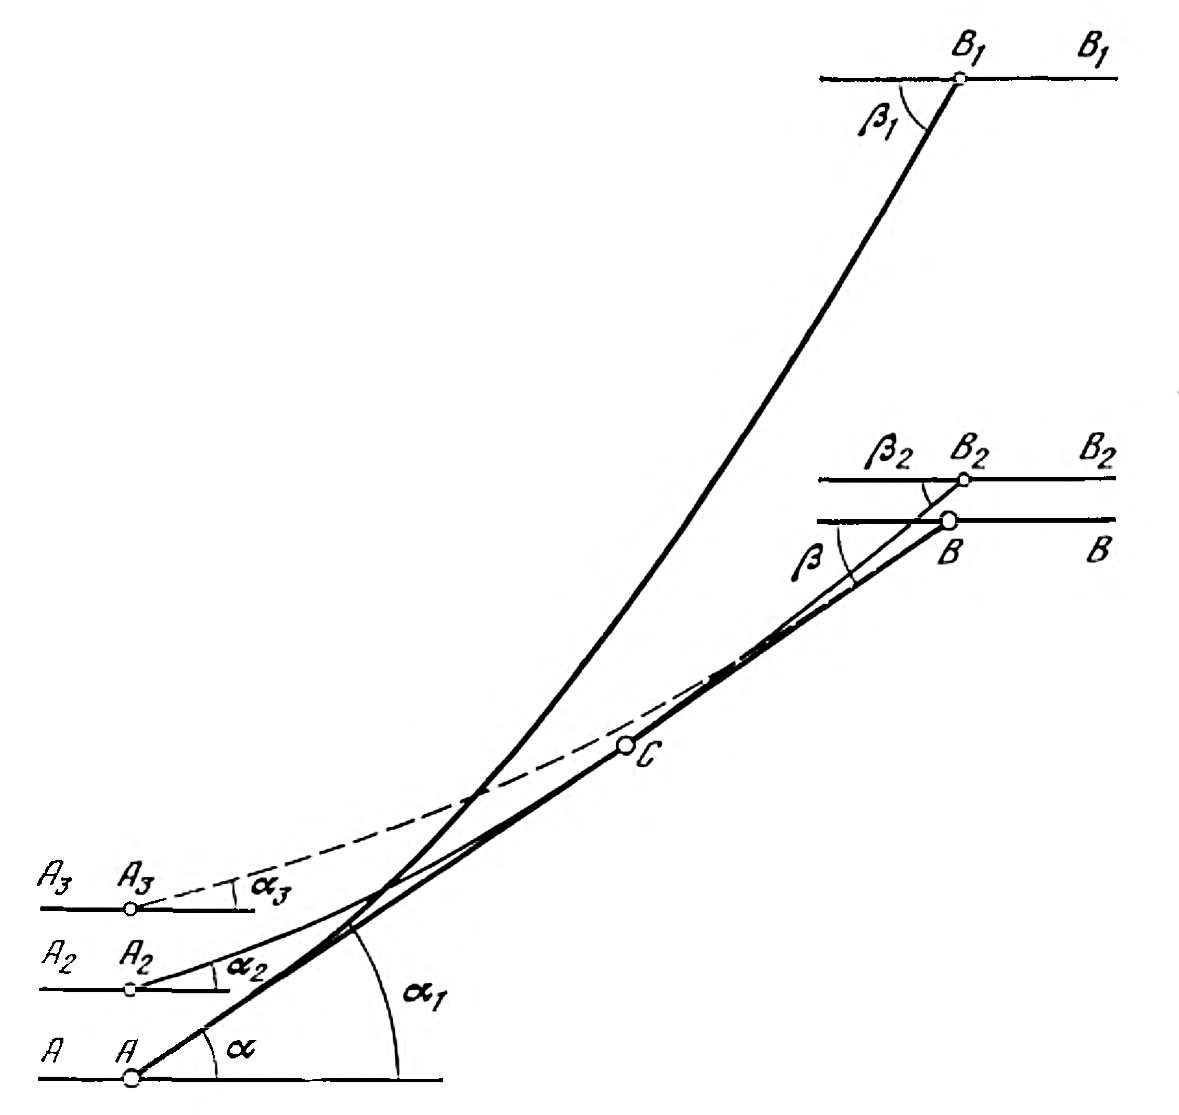
\includegraphics[width=0.85\linewidth]{figures/f9.1.png}
\end{figure}
\figblock{9.1}{Three variants of the zero-line image in perceptual perspective, depending
  on the reference depth~$l^*$.  Curve~$AB_1$ ($l^* = 0$): correct near ground but
  incorrect horizon angle.  Curve~$A_3B$ ($l^* \to \infty$): correct horizon angle but
  incorrect near-ground intersection.  Curve~$A_2B_2$ ($l^* = l^*$, intermediate):
  best compromise.  All curves are convex downward.}

Begin with the case $l^* = 0$.  Here the stretchings due to the size-constancy mechanism
yield the zero line as a curve~$AB_1$.  The angle~$\alpha_1$ of inclination of the zero
line to the picture base is unchanged compared with angle~$\alpha$ of the linear
perspective ($\alpha_1 = \alpha$).  It is important to note that both~$\alpha$ and the
appearance of downward convexity in the zero line fully correspond to visual perception,
as will be confirmed experimentally at the end of this Appendix.  However, if the zero
line is continued, the region near the horizon around point~$B_1$ will be distorted: the
angle between any line in the region of the horizon and the horizon line is always seen
exactly as in linear perspective, i.e.\ in the present case it should appear equal to~$\beta$,
whereas it turns out to be depicted as angle~$\beta_1 \neq \beta$.

\srcpage{283}

To avoid this, if one starts the construction from point~$B$, the horizon region is
depicted correctly, but in the near foreground the intersection of the new zero-line image
$A_3B$ with the lower edge of the picture~$A_3A_3$ occurs at angle~$\alpha_3 < \alpha$,
which contradicts visual perception.

Consequently, a perfect image of the zero line, taking into account not only linear
quantities but also angles, is excluded.  In this connection it may turn out that ``on
average'' the zero line is best transmitted if the starting point is~$C$ (curve~$A_2B_2$).
The angles of intersection of this curve with the lower edge~$A_2A_2$ ($\alpha_2$) and
with the horizon~$B_2B_2$ ($\beta_2$), although not corresponding to the visible angles
($\alpha_2 \neq \alpha$, $\beta_2 \neq \beta$), differ from them less than $\alpha_3$
and $\beta_1$ respectively.

\begin{figure}[H]
    \centering
    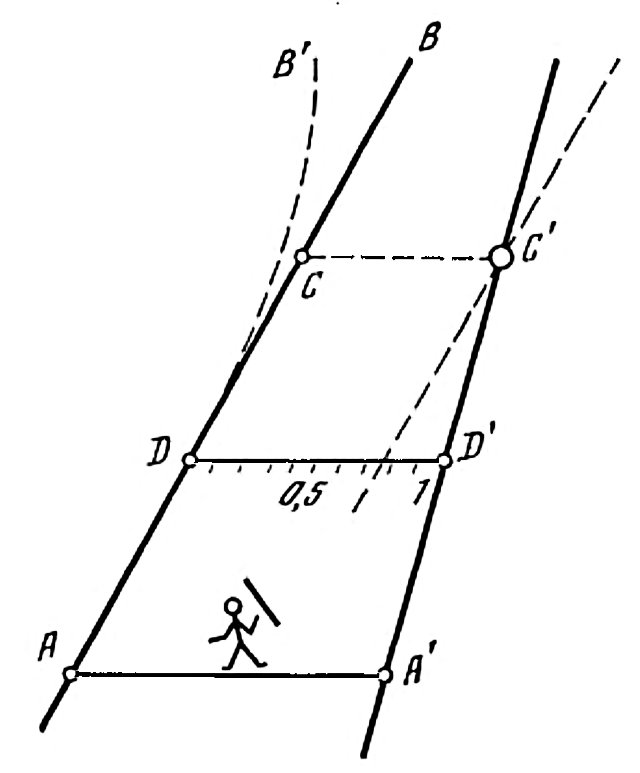
\includegraphics[width=0.45\linewidth]{figures/f9.2.png}
\end{figure}
\figblock{9.2}{Scheme of the experiment for measuring the curvature of a zero line
  observed in foreshortening.  The observer stands at the midpoint of strip~$AA_1$.
  Two readings of the ruler (aligned through~$C$, parallel first to~$OC$ and then to~$CB$)
  are compared; a difference indicates that the straight line~$OB$ of objective space is
  perceived as a curve in perceptual space.}

The actual curvature of zero lines observed in foreshortening can easily be registered
experimentally.  Fig.\,9.2 shows the scheme of the experiment.  The observer stands at the
midpoint of strip~$AA_1$.  The distance $AH = l_0$, and line~$OO'$ is graduated in
fractions of its length.  Object~$C$ is placed at the indicated position.  The ruler used
for sighting is held so that its trace on the ground appears to contain point~$C'$ and to
be parallel to the left side~$AB$ of the strip.  As can be seen, the experimental method
is the same as that described in Appendix~3.  The sole feature of the method is that
\emph{two} readings are taken: in the first, the ruler is held so that its trace on the
ground is parallel to~$OC$; in the second, so that it is parallel to~$CB$.  If the
straight line~$OB$ of perceptual space remains a straight line, there is no difference
between the first and second readings.  As experiment shows (conditions the same as those
described in Appendix~3 for $l_0 = 2$\,m), the first reading gives~0.765 and the second
0.866 (mean values from multiple readings by four observers at $l = 1$).  Consequently,
the objectively straight line~$OB$ turns out to be a curve in visual perception, shown
conventionally by the dashed curve~$OB'$.

% Appendix 10: Visual Representation of Sections of Four-Dimensional Space
% Source pages: 284–286

\chapter{Visual Representation of Sections of Four-Dimensional Space}

\srcpage{284}

The present Appendix is devoted to the visual representation of those aspects of the
geometry of multi-dimensional spaces that are essential for the considerations set forth
in Chapter~VII when describing the methods of simultaneously transmitting on the picture
plane the ordinary and the mystical space.  The necessary clarity can be achieved only
by simplifying the problem under consideration.  We use here an approach that is very
commonly applied for this purpose in geometric reasoning.  As already noted in
Chapter~VII, a visual representation of three-dimensional ``layers'' situated in
four-dimensional space is impossible.  We therefore consider an analogous problem,
passing to simpler spaces---two-dimensional and three-dimensional.

Suppose there exist two-dimensional beings living in a two-dimensional space---for
instance, some ``flat'' creatures that move only on a certain plane and do not know
that there is a third dimension in the world, i.e.\ they cannot even imagine motion
perpendicular to the plane on which they live.  Obviously, the movements of these flat
beings are described by two coordinates.  In contrast to these creatures, we
(three-dimensional beings) can readily visualise that, in addition to the named plane,
there may be another plane, parallel to the first, on which flat beings can also live.
Denote the first plane~$\pi_1$ and the second~$\pi_2$.  Whatever the distance between
$\pi_1$ and~$\pi_2$, the beings inhabiting them cannot pass from one plane to the
other, since they are unable to perform the motion perpendicular to the planes that
this would require.

An important special case of this example is that in which the distance between~$\pi_1$
and~$\pi_2$ is infinitely small.  Most simply, one may imagine the planes~$\pi_1$
and~$\pi_2$ to coincide but to belong to different sides---say, $\pi_1$ corresponds to
the ``upper'' and $\pi_2$ to the ``lower'' surface of some infinitely thin plane.  Then
a situation arises in which two groups of heterogeneous beings live on one plane; these
groups never meet one another, they can, without interfering with each other, occupy the
same regions of ``their'' two-dimensional space, and so on---all because they are
displaced relative to one another by an infinitely small distance, but in a direction
that is incomprehensible to them---the ``third'' direction.

\srcpage{285}

The constructed example is in essence analogous to that considered in Chapter~VII, where
the discussion concerned two three-dimensional spaces infinitely slightly displaced
relative to one another in the ``fourth'' direction, allowing two ``lives''---ordinary
and mystical---to exist in the same volume (of a room, for instance).  Obviously the
analogies can be extended: mystical and ordinary space are not completely independent,
they are linked not materially but spiritually (by prayer, etc.), but this too can be
supposed of the flat beings inhabiting the sides~$\pi_1$ and~$\pi_2$ of the introduced
plane.  Further, if one allows that in certain exceptional cases the flat beings of~$\pi_1$
can ``seep through'' from the ``upper'' to the ``lower'' surface, they will possess the
ability to ``appear'' to the beings of~$\pi_2$ ``from nothing'', and so on.

For the problem under consideration here, what matters is not the analogies of the
properties of the complex of ordinary and mystical spaces and those of the two sides
($\pi_1$ and~$\pi_2$) of a single plane, but rather the rational methods of \emph{depicting}
such two spaces.  Begin with the vivid example of a two-sided plane.  Since a drawing
is always one-sided, the only way of simultaneously depicting the sides~$\pi_1$ and~$\pi_2$
on a drawing (without the depicted sides overlapping one another) is the \emph{method of
sections}: wherever the side~$\pi_1$ is depicted, the depiction of~$\pi_2$ must be
interrupted, and to facilitate their distinction the images of sides~$\pi_1$ and~$\pi_2$
should be painted in different colours.  Precisely the same procedure must be used when
depicting events occurring in two infinitely close three-dimensional ``layers'' of a
four-dimensional space: if one builds a visual three-dimensional model of such a space,
some regions of the model's volume must be assigned to conveying the ordinary space,
while in other regions of the model the mystical space is depicted.  As is clear from
what has been said, this is also the method of sections: two coexisting three-dimensional
spaces are shown alternately.

The transfer of such a three-dimensional model onto a picture plane (for instance, an
icon) no longer differs in any way from any other depiction of some three-dimensional
space, since the method of sections has reduced the task of conveying the geometry of two
three-dimensional ``layers'' of a four-dimensional space to the task of conveying the
geometry of a three-dimensional space in which sections of these ``layers'' neighbour one
another rather than ``overlapping'' one another.

\srcpage{286}

Of course, the method of sections is unable to show simultaneously both the ordinary and
the mystical spaces across the whole picture plane (just as one cannot show both sides of
a two-sided plane on one side of a drawing), but the possibility of simultaneously showing
both named spaces, even partially, is often more important than a complete depiction of
either one of these two spaces alone.

% Appendix 11: The Form-Constancy Mechanism and Portrait Painting
% Source pages: 286–287

\chapter{The Form-Constancy Mechanism and Portrait Painting}

The well-known artistic effect by which the person depicted in a portrait ``follows the
viewer with his eyes'' as the viewer moves can be amplified, so that the portrait begins
to ``turn with its whole body'' within the frame in pursuit of the viewer.  Such mobility
of the depicted person can be explained by the action of the form-constancy mechanism.

Fig.\,11.1 shows a schematic representation (view from above) of a portrait~$b$ hanging
on wall~$a$.  When the viewer occupies position~$A$, i.e.\ his gaze makes a right angle
with the plane of the picture (and of the wall), he sees the image as the artist created
it.  When the viewer moves to position~$B$ or~$C$, his gaze makes an acute angle~$\alpha$
with the plane of the wall and picture.  In this case the retinal image of the picture is
strongly distorted compared with that corresponding to position~$A$.

\begin{figure}[H]
    \centering
    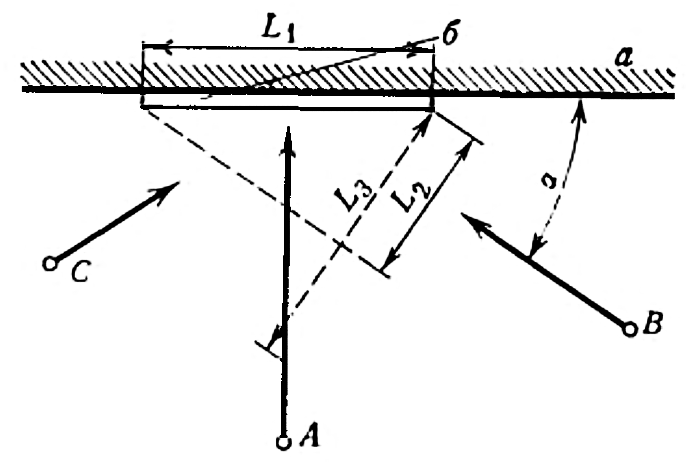
\includegraphics[width=0.6\linewidth]{figures/f11.1.png}
\end{figure}
\figblock{11.1}{View from above.  Portrait~$b$ hangs on wall~$a$.  At position~$A$ the
  gaze is normal to the picture plane.  At position~$B$ or~$C$ the gaze makes acute
  angle~$\alpha$ with the wall; the form-constancy mechanism ``stretches'' the retinal
  image horizontally from width~$b_1$ to~$b_3$, effectively rotating the depicted person
  to face the viewer.}

Since every person has excellent knowledge of the ``geometry'' of a human face, its
distortion due to the deviation of~$\alpha$ from a right angle is immediately
subconsciously compensated by the form-constancy mechanism: this mechanism as it were
``stretches'' the retinal image of the picture horizontally to the width~$b_3$ at which
the face appears in its usual form.  Clearly $b_3 \gg b_1$.  Taken together, this effect
leads to an apparent rotation of the whole image perpendicular to the line of sight from
point~$B$.

\srcpage{287}

Now consider the transformation of the appearance of wall~$a$.

If the system of wall~$a$ and portrait~$b$ is observed simultaneously, two cases are
possible.  If the picture frame is perceived as an element of the picture itself, the
form-constancy mechanism simply allows looking at the picture at sufficiently acute
angles~$\alpha$.  In those (comparatively rare) cases where the artist succeeds in
``uncoupling'' the portrait from the frame---making the frame be subconsciously perceived
as part of the wall rather than of the picture---the described ``rotations'' of the image
will be perceived as rotations relative to the picture frame, and the portrait will
``follow'' the viewer not only with the eyes but through apparent turns of the face and
body relative to the frame.

The question of what artistic means allow one to ``uncouple'' portrait from frame is not
considered here.  We note only that the apparent rotation is impeded by a frontal
depiction of the sitter, in which the line of the shoulders is parallel to the picture
plane: this as it were ``anchors'' the sitter to the picture plane defined by the frame.
In those cases where the artist places the sitter so that his shoulder line is
approximately perpendicular to the picture plane, and simultaneously removes everything
that might ``anchor'' the depicted person to that plane, the effect of ``rotations'' of
the portrait relative to the frame is very easily observed.  The described property is
possessed by such portraits as the \emph{Lady with an Ermine} by Leonardo da Vinci and
many others.

If one limits oneself to the collection of the State Tretyakov Gallery alone, one may
cite the portrait of Baryatinsky by Rokotov, the portrait of Derzhavina by Borovikovsky,
the portraits of Rostopchina by Kiprensky and of Putyatina by Venetsianov.  The same
property belongs to Tropinin's painting \emph{Boy with a Zhaleika} and to a number of
other works.


\end{document}
